% !BIB TS-program = biber
% !BIB program = biber
\title{From Context Transformation Algorithm \\ to $N^\ast$ model of Set Theory}
\author{
        Yauhen Yakimovich\footnote{Please see the end of the paper for Acknowledgements} \\ \href{mailto:yauhen.yakimovich.mail@gmail.com}{yauhen.yakimovich.mail@gmail.com}
}


\documentclass[english,a4paper,11pt,oneside]{article}

% Many custom declarations and package usages
%\documentclass[sigconf,natbib=false]{acmart}
% ---------------------------
% \usepackage[utf8]{inputenc}
\usepackage[english]{babel}

% \babelprovide[import]{hebrew}
%\babelprovide[onchar=fonts ids]{hebrew}
% \babelfont[hebrew]{rm}[SlantedFont = SILEOT]{SILEOT.ttf}

\usepackage{csquotes}
% ---

\usepackage{datetime}
\usepackage{hyperref}
\usepackage{float}
\usepackage{graphicx}
\usepackage{subcaption}
\usepackage[hyperref = true,
  backref = true,
  backend = bibtex,
  style = nature,
	sorting = none,
]{biblatex}

% FIXME:
\usepackage{mathalpha}
\usepackage{mathtools}
% \usepackage{stix2}

\usepackage{amsmath}
\usepackage{amsthm}
\usepackage{amssymb}
\usepackage{stmaryrd}

\usepackage{tikz-cd} % For commutative diagrams

% https://mirror.foobar.to/CTAN/macros/latex/contrib/mathalpha/doc/mathalpha-doc.pdf
% \DeclareMathAlphabet\mathbfcal{LS2}{stixcal}{b}{n}
\DeclareMathAlphabet\mathbfcal{OMS}{cmsy}{b}{n}

% ---------------------------
\usepackage[shortlabels]{enumitem} 
\usepackage{listings}
\usepackage{color}
\usepackage{appendix}
\usepackage[normalem]{ulem}
\usepackage{makecell}

%-----------------------------
% sub-"enumerate" with enumitem
\newlist{legal}{enumerate}{10}
\setlist[legal]{label*=\arabic*.}
%-----------------------------

\date{\displaydate{date}}
\date{\today\\v1.0.0}

\definecolor{somegreen}{rgb}{0,0.6,0}
\definecolor{somegray}{rgb}{0.5,0.5,0.5}
\definecolor{mymauve}{rgb}{0.58,0,0.82}

\lstset{ 
  backgroundcolor=\color{white},   % choose the background color; you must add \usepackage{color} or \usepackage{xcolor}; should come as last argument
  basicstyle=\footnotesize,        % the size of the fonts that are used for the code
  breakatwhitespace=false,         % sets if automatic breaks should only happen at whitespace
  breaklines=true,                 % sets automatic line breaking
  captionpos=b,                    % sets the caption-position to bottom
  commentstyle=\color{somegreen},    % comment style
  deletekeywords={...},            % if you want to delete keywords from the given language
  escapeinside={\%*}{*)},          % if you want to add LaTeX within your code
  extendedchars=true,              % lets you use non-ASCII characters; for 8-bits encodings only, does not work with UTF-8
  firstnumber=1000,                % start line enumeration with line 1000
  frame=single,	                   % adds a frame around the code
  keepspaces=true,                 % keeps spaces in text, useful for keeping indentation of code (possibly needs columns=flexible)
  keywordstyle=\color{blue},       % keyword style
  language=C++,		               % the language of the code
  morekeywords={*,...,contract,function,returns},            % if you want to add more keywords to the set
  numbers=left,                    % where to put the line-numbers; possible values are (none, left, right)
  numbersep=5pt,                   % how far the line-numbers are from the code
  numberstyle=\tiny\color{somegray}, % the style that is used for the line-numbers
  rulecolor=\color{black},         % if not set, the frame-color may be changed on line-breaks within not-black text (e.g. comments (green here))
  showspaces=false,                % show spaces everywhere adding particular underscores; it overrides 'showstringspaces'
  showstringspaces=false,          % underline spaces within strings only
  showtabs=false,                  % show tabs within strings adding particular underscores
  stepnumber=2,                    % the step between two line-numbers. If it's 1, each line will be numbered
  stringstyle=\color{mymauve},     % string literal style
  tabsize=2,	                   % sets default tabsize to 2 spaces
  title=\lstname                   % show the filename of files included with \lstinputlisting; also try caption instead of title
}

\newtheoremstyle{mydef}
{\topsep}{\topsep}%
{}{}%i
{\bfseries}{}
{\newline}
{%
  \rule{\textwidth}{0.4pt}\\*%
  \thmname{#1}~\thmnumber{#2}\thmnote{\ -\ #3}.\\*[-1.5ex]%
  \rule{\textwidth}{0.4pt}}%

\theoremstyle{mydef}
\newtheorem{definition}{Definition}
\newtheorem{theorem}{Theorem}
\newtheorem{claim}[theorem]{Claim}
\newtheorem{proposition}[theorem]{Proposition}
\newtheorem{lemma}[theorem]{Lemma}
\newtheorem{corollary}[theorem]{Corollary}
\newtheorem{conjecture}[theorem]{Conjecture}
\newtheorem{observation}{Observation}
\newtheorem{principle}{Principle}
\newtheorem*{example}{Example}
\newtheorem*{remark}{Remark}
\newtheorem*{axiom}{Axiom}

% also see options for fonts in latex 
% https://tex.stackexchange.com/questions/58098/what-are-all-the-font-styles-i-can-use-in-math-mode
\newcommand*{\numberset}[1]{\mathbb{#1}} 
\newcommand{\nat}{\numberset{N}}
\newcommand{\integers}{\numberset{Z}}
\newcommand{\rationals}{\numberset{Q}}
\newcommand{\reals}{\numberset{R}}
\newcommand{\cset}{\mathcal{C}}
\newcommand{\bin}{\mathcal{B}}
\newcommand{\cbin}{\numberset{B}}
\newcommand{\pset}{\mathcal{P}}
\newcommand{\yset}{\mathcal{Y}}
\newcommand{\rset}{\mathcal{R}}
\newcommand{\porder}{\mathbb{P}}
\newcommand{\cont}{\mathfrak{c}}
\newcommand{\mcar}{\mathfrak{m}}
\newcommand{\cesef}{\mathrm{E}_{SEF}} % countable list of all labels of eq classes over all fin formulas
\newcommand{\uesef}{\mathcal{E}_{SEF}} % uncountable list of all labels of eq classes over all infinite formulas
\newcommand{\ufsef}{\mathcal{F}_{SEF}} % uncountable list of fair formulas
\newcommand{\uusef}{\mathcal{U}_{SEF}} % uncountable list of unfair formulas
\newcommand{\vsef}{\mathbb{S}} % syntactically valid SEFs
\newcommand{\vhsef}{\mathbb{T}} % cumulative hierarchy syntactically valid SEFs

\newcommand{\lsef}{L_{SEF}}  % countable list of all finite formulas
\newcommand{\ulsef}{\mathcal{L}_{SEF}}  % uncountable list of all infinite (countable) formulas

\newcommand{\psf}{\mathfrak{F}} % probability space: field of sets - events

% model theory
\newcommand{\lsign}{\mathbfcal{L}}  % L-signature or L language
\newcommand{\Lf}{\mathbfcal{F}}  % Functions
\newcommand{\Lr}{\mathbfcal{R}}  % Relations
\newcommand{\Lc}{\mathbfcal{C}}  % Constants
\newcommand{\LsT}{\mathbfcal{T}}  % L-theory
\newcommand{\LsA}{\mathbfcal{A}}  % L-structure
\newcommand{\LsB}{\mathbfcal{B}}  % L-structure
\newcommand{\LsN}{\mathbfcal{N}}  % L-structure
\newcommand{\LsM}{\mathbfcal{M}}  % L-structure
\newcommand{\LsQ}{\mathbfcal{Q}}  % L-structure
\newcommand{\LsV}{\mathbfcal{V}}  % L-structure
\newcommand{\LsS}{\mathbfcal{S}}  % L-structure

% for boolean lagebra signature
\newcommand{\bF}{\textbf{0}}  % algebra structure
\newcommand{\bT}{\textbf{1}}  % algebra structure

\newcommand{\notimplies}{\;\not\!\!\!\implies}
\newcommand{\substr}{\ \varepsilon\ }

% some extended hebrew notation
% \newcommand{\HebrewLetterAsMathSymbol}[1]{\text{\foreignlanguage{hebrew}{#1}}}
% \newcommand{\hebhe}{\HebrewLetterAsMathSymbol{ה}} % 5
% \newcommand{\hebvav}{\HebrewLetterAsMathSymbol{ו}} % 6
% \newcommand{\hebzayin}{\HebrewLetterAsMathSymbol{ז}} % 7  
% \newcommand{\hebchet}{\HebrewLetterAsMathSymbol{ח}} % 8
% \newcommand{\hebtet}{\HebrewLetterAsMathSymbol{ט}} % 9
% \newcommand{\hebtav}{\HebrewLetterAsMathSymbol{ת}} % 22


% function restriction
\newcommand\restr[2]{{% we make the whole thing an ordinary symbol
  \left.\kern-\nulldelimiterspace % automatically resize the bar with \right
  #1 % the function
  \vphantom{\big|} % pretend it's a little taller at normal size
  \right|_{#2} % this is the delimiter
  }}

% use quotes in math mode to define strings
%\DeclareMathSymbol{\mlq}{\mathord}{operators}{"}
%\DeclareMathSymbol{\mrq}{\mathord}{operators}{"}
\newcommand{\bos}{\text{``}}
\newcommand{\eos}{\text{''}}

% complement
\newcommand{\stcomp}[1]{{#1}^\complement}

% bij 
\newcommand\bij{\lhook\joinrel\twoheadrightarrow}

% cupdot disjoint union UPDATE: defined by stix2
\newcommand{\cupdot}{\mathbin{\mathaccent\cdot\cup}}
\newcommand{\fdot}{\mathbin{\mathaccent\cdot F}} % uncomputable fair

% Inserts \clearpage before \begin{appendices}
\BeforeBeginEnvironment{appendices}{\clearpage}
% Inserts \clearpage after \end{appendices}
%\AfterEndEnvironment{appendices}{\clearpage}

% Inserts \clearpage before every \section within appendices environment
%\AtBeginEnvironment{appendices}{\pretocmd{\section}{\clearpage}{}{}}{}

% doted curly wedge and vee
\newcommand{\cdwedge}{\dot{\curlywedge}}
\newcommand{\cdvee}{\dot{\curlyvee}}

% nand
\newcommand{\nand}{\barwedge}


\addbibresource{paper.bib}

\begin{document}

\selectlanguage{english}

\begin{titlepage}
  \clearpage\maketitle
  \thispagestyle{empty}

  \begin{abstract}
    This paper proposes Set Theory models \( N \) of \( ZF + DC \) that explicitly decides the Continuum Hypothesis ($CH$) as well as \( N^\ast \) of \( ZF + DC_\lambda + I \) that implies the existence of \textit{supercompact cardinal}. The approach employs advanced and somewhat novel techniques from mathematical logic, including Boolean-valued models and String Enumeration Formulas (SEF) to build \textit{replicata} structures as used for the models. It follows that $CH$ becomes resolved for all instances of large enough models of \( ZF + DC \), providing a concrete solution to a longstanding open problem, so that Goedel's conjecture $2^{\aleph_0} = \aleph_2$ holds. Other results offer new insights into the structure of \( N^\ast \) and its implications for related mathematical theories, laying a foundation for further research on infinite sets.
  \end{abstract}
\end{titlepage}

\pagebreak

\tableofcontents

\pagebreak

\pagebreak
\hspace*{\fill}\textit{For Mary and Emilia}

\pagebreak
\section{Preface}

Embarking on the exploration of a simple algorithm years ago marked the beginning of an extraordinary journey for me. This quest soon transformed not only into a hobby, but rather what I affectionately refer to as my favorite long-term relationship. Back in 2007, as a software engineer with practical experience in the industry, I found myself increasingly drawn to the theoretical aspects of mathematics, eventually developing a keen interest in Set Theory.

The concept of applying the CTA algorithm in an infinite context did not emerge suddenly. Instead, it was a gradual realization, spurred by my encounter with Cantor's diagonal argument (which to my shame I completely misunderstood at first and was able to fully comprehend only years after graduating in technical field). This personal discovery was a significant turning point, opening up the new and unknown realm of infinite for me. 

My initial intention was purely educational, aimed at expanding my understanding as much as possible. Over the years, this scholarly pursuit evolved. I gathered my scattered notes, gradually mustering the courage to compile them into a coherent manuscript. The objective was to produce a concise paper, offering a computer science perspective on the notion of infinities, particularly in relation to the continuum hypothesis.

However, as time passed, it became painfully clear through numerous trials and errors that a computer science lens alone was inadequate. It lacked the necessary precision not just for answering questions, but even for formulating them correctly. This realization necessitated a deeper, more fundamental approach to learning.

A pivotal moment in my journey was the acknowledgement that disproving the continuum hypothesis (CH) or proposing a naive theoretical example of its possibility was not a novel achievement. Paul Cohen's groundbreaking 1963 paper, which elegantly and rigorously demonstrated the independence of CH using the sophisticated method of forcing, was a humbling reminder of the complexity of these problems.

Despite these challenges, I remained motivated by the belief that my unique approach might still offer a fresh perspective or become a useful tool in the field. This paper is the result of years of learning, exploring, and refining these ideas.

Now, as I conclude this draft, I am ready to present my findings. This paper represents not just an academic endeavor, but also a personal journey from a software engineering background into the depths of mathematical theory.


\section{Introduction}

Traversing a binary string is a process that is trivial enough to imagine.  This is equivalent to enumerating some sequence of values. Each value can be either zero or one. The process of enumerating such values allows labeling each position with a number or an \textit{index}, so that we can always find out the value at certain position. A sequence of $\{0,1\}$ equipped with such indexing will then be a binary string, but the same can be stated more formally.

\begin{definition}\label{def_binstr}
    If the position of each value of some binary sequence can be enumerated by an index set $J\subseteq \nat$, so that each index can be mapped to the binary value at the respective position, then we call such mapping $b : J \to \{0, 1\}$ a binary string.
\end{definition}

Existence of the above mapping also means that the binary string $b$ has the same ``cardinality'' as its index set $J$. We call such ``cardinality'' \textit{the length of the binary string} and denote this as $|b| = |J|$. For example, if some string $b$ has the length $n\in \nat$, then this fact is noted as $|b| = n$ or with the lower subindex $b_n$.

Sometimes we also use round bracket or double quote notation if we need to explicitly indicate which exact finite sequence of $\{0, 1\}$ does represent some concrete binary string. For example, the following notations of a binary string $b_n$ are equivalent and ordered by increasing brevity:

\begin{itemize}
    \item[$\backsim$] $(1,0,0,1,1,1,0,1,..,0,1,1)_n$
    \item[$\backsim$] $\bos1,0,0,1,1,1,0,1,..,0,1,1\eos_n$
    \item[$\backsim$] $\bos10011101..011\eos_n$
    \item[$\backsim$] $10011101..011_n$
\end{itemize}

A set of binary strings that have the same length is denoted as $B_n = \{ b_n \in \big| n \in \nat \}$.

\begin{definition}
    Consider a set of binary strings $B_n$ of a finite length $n$ from $2^n$ of possible strings of that length, $\ s.t.\ |B_n| = 2^n$. We say that two strings $x_n \in B_n$ and $y_n \in B_n$ are \textit{equal} iff values in both strings are equal at each position $j$ as in $x_n(j) = y_n(j), \forall j \in J $, where $J$ is some index set shared by $x_n$ and $y_n$.
\end{definition}

By analogy of the opposite, the \textit{inequality} of $x_n,y_n \in B_n$ follows from $\exists j, j \in J: x_n(j) \neq y_n(j).$

Given the above definitions we are going to look at binary strings of some finite length in the first part of the paper and consider context dependent transformation of their values called \textit{context transformation algorithm} (CTA). In the second part of the paper we will discuss CTA applications to more fundamental concepts such as cardinality of infinite binary strings. Some other generalizations of the CTA as well as listings of code are provided in appendix of this paper.

\pagebreak
\section{Finite case of CTA}

\subsection{Context depended operations}

Following earlier definitions one can proceed with some basic transformations of binary strings. Consider a boolean logic operation like $xor$ computed over values of two strings $\{x_n, y_n\} \subset B_n, n \in \nat$ individually. The result of such string operation $z_n$ can be obtained as value-wise or element-wise addition modulo 2, s.t. $z_n(j) = x_n(j) \oplus y_n(j), \forall j \in J $, where $J$ is an enumeration or index set. 

Computing a sequence $z_n(j), \forall j \in J$ is done index by index, defined by the shared enumeration set $J$ with each position being treated independently. Meaning that the end result does not depend on the order of operations as long as the bits of the outcome binary string $z_n$ can be put together in the right order $\forall j \in J$. We will call such operations \textit{context-free operations}. 

A different situation is a special case when some basic binary operation is applied to strings of bits in strictly dependent order. Indeed, the trivial case of performing a $xor$ operation over two binary strings can be computed in parallel and the outcome will be always the same over and over again as long as we can match the indexes. 

However, if one can control how the resulting $z_n$ string is produced by adding some memory property to store previously computed or observed states, one will most likely come up with a stateful process of a binary string transformation. We will refer to such string operations augmented with the memory state as \textit{context depended operations}.

\begin{definition}\label{def_cursor}
  Consider an input binary string $b_n, n \in \nat$ and a cursor $b_n(k)$ pointing at some index $0 \leq k < n$. A context of a fixed length $m < n$ observed to the left of $k$ is a \textit{prefix} enumerating values before index $k$ as $\bos b_n(k-m),..,b_n(k-1)\eos.$
\end{definition}

\subsection{Context Transformation Algorithm}

Let us illustrate how one of such context depended algorithms can work. Let $b_n$ be a finite input string. We will use a state lookup table (see fig. \ref{fig:cta}) for state tracking purposes. One needs to choose the length of the context as $m < n, m \in \nat$, so that the left-hand of the lookup table will consists of all possible context strings of such length $C_m = \{\bos 000..00\eos_m, \bos 000..01\eos_m, .. \\ \bos 111..11\eos_m\},\, |C_m| = 2^m$ that can be potentially found while traversing $b_n$ with $k \in J = \bos 0,\,..,\,n-1\eos$. 

\begin{figure}[h!]
  \centering
  \begin{subfigure}[b]{0.9\linewidth}
    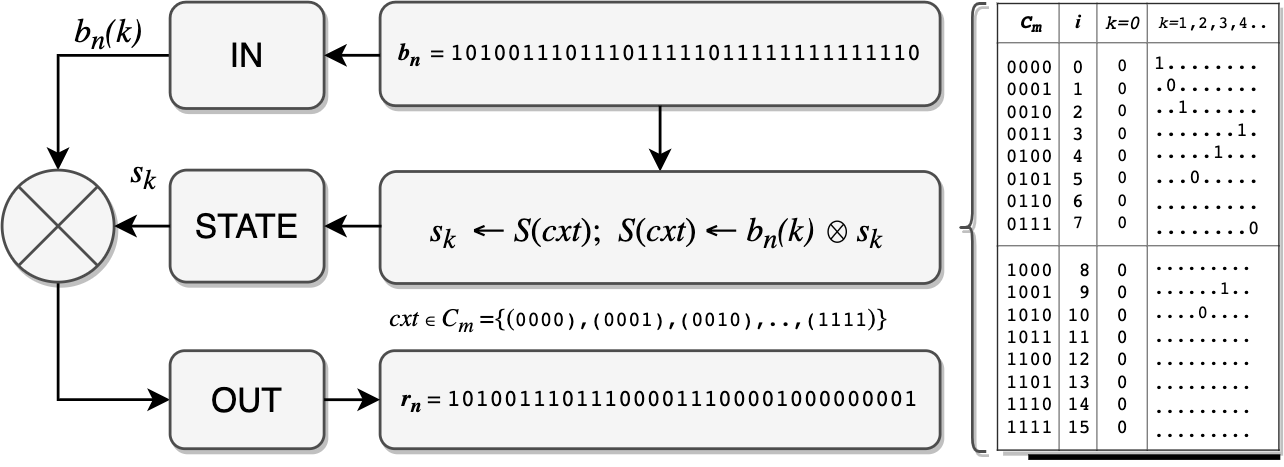
\includegraphics[width=\linewidth]{appendix/CTA.png}
  \end{subfigure}
  \caption{Context transformation algorithm. Finite case.}
  \label{fig:cta}
\end{figure}

For convenience, prefix values which have not yet been observed before some cursor $k < m$ are padded with zeros. For example, for $k \geq 0$ and $m=4$ first few observed context strings will be padded until no more padding is required as in $(0000, 000x, 00xx, 0xxx, xxxx)$, where $x \in \{0,1\}$ is a value placeholder and $k \geq m$. Alternatively one can imaging a sliding window of fixed length $m < n$ moving from left to right over the indexes of $b_n$ to observe all found context strings of that length.

We define a finite case of \textit{CTA} as following: 

\begin{enumerate}
\item \textbf{take} a finite binary string $b_n$ as input - for example,\\ let $b_n = \bos101001110111011111011111111111110\eos_{n=33}$
\item \textbf{choose} the size of the context as $m < n, m \in \nat$ - for example, $m=4$
\item \textbf{point} cursor at position $k=0,k \in J$, so that we can access first value $1 \leftarrow b_n(k)$ at the beginning of $b_n$
\item \textbf{initialize} all unobserved states in the state table with zeros \\$S(cxt) \leftarrow 0, \forall cxt \in C_m$ 
\item \textbf{set} the observed context $cxt \leftarrow \bos 000..00\eos_m$
\item \textbf{shift} bits of the observed context to the left by dropping a value at the first index $cxt(0)$ 
\item \textbf{update} the observed context string by appending the input value at cursor $cxt \leftarrow \bos cxt(1), cxt(2), .., cxt(m-1), b_n(k)\eos_m$
\item \textbf{take} $s_k \leftarrow S(cxt)$
\item \textbf{output} next bit $r_n(k) \leftarrow b_n(k) \oplus s_k$
\item \textbf{update} memory state for observed context $S(cxt) \leftarrow b_n(k) \oplus s_k$, which will be $1$ if the state has changed and $0$ otherwise
\item \textbf{if} $k = n$ and cursor points at the end of the input string, 
\\ \textbf{then} transformation is complete and we can terminate the algorithm
\\ \textbf{else} move cursor to the next index $ k \leftarrow k + 1$ at the input string $b_n$ (from left to right) and continue by jumping back to step (6) 
\end{enumerate}

\subsection{Bijectivity of CTA}

Above we have defined the CTA as a context-depended algorithm that takes a finite binary string $b_n$ as an input and uses a simple $xor$ operation applied to the input bits and the memory states to produce an output string $r_n$. For example and as shown on fig. \ref{fig:cta} - $r_n \leftarrow CTA(b_n)$, so for the sample input the CTA result is: \begin{align*}
b_n = \bos101001110111011111011111111111110\eos
\\ r_n = \bos101001110111000011100001000000001\eos
\end{align*}

Interestingly enough, $xor$ operation on binary strings can be easily reversed. Which means, that one can also define an inverse version of the algorithm such that it will take $r_n$ as input and produce the original values of $b_n$ as output - $b_n \leftarrow {CTA}^{-1}(r_n)$.

\begin{theorem}If a context transformation algorithm on finite binary strings $B_n$ can be represented by a function ${CTA}_{m}: B_n \to B_n$, where context length is $m < n: m,n \in \nat$, then ${CTA}_{m}$ is both a total computable and bijective function.\end{theorem}
\begin{proof}There exists a direct and inverse implementation of ${CTA}_{m}$ in Turing-complete programming language\footnote{See "CTA - code listing" in appendix - for direct and inverse algorithm implementation in python}.\end{proof}



\pagebreak
\section{Countable case of CTA}

\subsection{Infinite binary strings}

So far we have looked at binary strings of finite length. Sets of such strings have been arranged as binary tables over which we run a context-depend transformation to produce an output binary string. Next we will see that sequences of $\{0,1\}$ can be considered to be rather ``large'' or unrestricted. For example, not only input and output binary strings, but also individual rows in such tables can be repeatedly padded by zeros or any other algorithmically printable patterns consisting of finite substrings. 

Instead of trying to print all of the elements at once of any such cyclic binary string in a single infinite loop, it would be much more pragmatic to approximate the process by printing out only finite subparts of an infinite string that are accessed at particular indexes $\forall j \in J$. For example, when accessing the subsets or snapshots of the values to be printed out or when implementing a tape to store a value using Turing Machine (TM). In other words, those values can be reached and printed out within a certain computational time\footnote{or within other reasonable constraints depending on the needs of the respective computational model if it is different from the deterministic TM}. We will agree that such access is happening by means of a \textit{cursor} $b(j), \forall j \in J$ - a totally computable function that takes index as an input to return the desired value. We will also refer to such selective access of cyclic binary strings as \textit{algorithmic access}. 

\begin{definition}If there exists an algorithm such as a cursor function $b(j), \forall j \in J$ that can \textit{access} some values of an infinite binary string by printing them out, we say about those values that they are \textit{algorithmically reachable}.\end{definition}

Indeed, it is easy to construct a function that will map a sequence of natural numbers to a totally ordered set of binary strings. Such function will be merely a translation from each natural number into a binary format which are padded with zeros (or some repeatable pattern). This fact can be noted as one of the possible enumerations of any infinitely countable set of numbers\footnote{such countable set can be defined as a \textit{proper set} depending on the consistency needs of the logical foundation or computational framework, since we don't require infinitely countable set of binary strings to contain all possible variations of binary strings - see section \textit{4.4 Uncountable cardinalities}} by a list of binary strings with \textit{one-to-one} and \textit{onto} correspondence.

\begin{lemma}If $\bin$ is an infinitely countable set of binary strings, then any enumeration of those strings produces an index set $I\subseteq \nat$, where $\kappa : I \to \bin$ is some particular enumeration of $\bin$.\end{lemma}

To simplify the notation, the length of the individual string $b \in \bin$ is not restricted with any finite $n \in \nat$ and the infinite padding is assumed if needed for the algorithmic access of values such as $b(j), j \in J$. It is easy to show that any finite non-cyclic part of such string can be algorithmically accessed as well\footnote{as long as there is enough memory to store the unique finite substring or it can be produced algorithmically as with translation of any natural number into a binary format}. More formally this can be stated as following:

\begin{definition}A string $b$ is called semi-open\footnote{as without end at least once} and infinitely countable on the left (right) or \textit{left-infinite} (respectively, \textit{right-infinite}), for short, iff there exists a bijective mapping $\alpha : \nat \to J$, such that any index $\forall j = \alpha(n), n \in \nat$ can access all values in $b$ as in $b(j) = b(\alpha(n))$ starting from the right bits towards countably many on the left side of the string (respectively, $\exists\, \sigma(n): \nat \to J$, which is bijective and can access values $b(\sigma(n)): n \in \nat$ starting from the left bits towards countably many on the right side of the string).\end{definition}


\begin{definition}A string $b$ is called open and \textit{bi-infinite} iff it does not have a start and an end and is both left- and right-infinite.\end{definition}

By choosing yet a different way to index or map values, one can consider equally infinite strings which would be closed, instead of being open. Obviously closed bi-infinite strings are similar up to isomorphism of a particular mapping to the open bi-infinite strings - a form, which we adopt through the rest of our discussion and without loss of any generality.

\begin{lemma}Let $o$ be open bi-infinite, $c$ - closed bi-infinite and $l, r$ be respectively left- and right-infinite binary strings. It is easy to show that $c,l,o,r$ share the same cardinality equal to that of $|\nat|$ or countable cardinality.\end{lemma} 

In order to show the last statement, it is enough to observe that $o$ can be indexed by some $J \subseteq \integers: |J| = |\integers| = |\nat|$.

\subsection{Generalized Context Transformation Algorithm}\label{subsec_gcta}

We will generalize CTA and apply it for a bi-infinite string $b: K \to \{0,1\}, K \subseteq \integers$  as an input. Let us start by considering a trivial case when $b$ has a form of $\bos..01010101..\eos$ sequence built by an infinite repetition of the $(01)$ pattern in both left and right directions. In order to produce the output string, we will apply the generalized context transformation algorithm (GCTA) by starting somewhere in the middle of $b$ and moving from left to right. Then we construct a GCTA table $T: (i,j) \to \{0,1\}$ with rows indexed by $i \in I, I \subseteq \nat$ and columns by $j \in J, J \subseteq \integers$.

\begin{definition}Let $b$ be a bi-infinite binary string with the cursor pointing at some index $k \in K, K \subseteq \integers$ somewhere in the middle of the string. A context observed to the left of $k$ or a \textit{prefix} is a left-infinite string equal to $b$ and obtained by ignoring\footnote{cutting off} all the values after the cursor starting with k as in $\bos k, k+1, k+2, k+3, ..\eos$.\end{definition}

The left-hand of the table $T(i,j), j < 0$ consists of left-infinite strings $\{cxt_i\}, i \in I$ in order to track the already observed prefixes in $b$ on the left. Let the cursor point at $k \in K, K \subseteq \integers$, so that we can access the values $\bos..,0 \leftarrow b(k-2), 1 \leftarrow b(k-1), 0 \leftarrow b(k), 1 \leftarrow b(k+1), 0 \leftarrow b(k+2),..\eos$ and so on. We can add a first entry into the left-hand part of the table which would be  $\bos..01010101\eos$. As we move the cursor to the next position towards right $1 \leftarrow b(k+1)$, the next prefix to add into the left-hand part of $T(i,j), j < 0$ would be $\bos..10101010\eos$. 

The right-hand of the GCTA table would consists of right-infinite strings. Values of those strings would be state sequences tracked as 
\begin{equation}s_{i,j + 1} \leftarrow S(j|cxt_i) \oplus b(k)\end{equation} 
where $(i,j \geq 0), i \in I, j \in J$ are the indexes over the occurred transformations given the respective left-infinite context $cxt_i = (T(i, j): i \in I, j < 0)$. 

\begin{lemma}If GCTA table can be built by traversing the input string $b$, then $\exists \mu: k \rightarrow (i,j)$, s.t. input string index $k \in K, K \subseteq \integers$ can be always mapped to GCTA table indexes $(i,j)$ by looking up the context $cxt_i$ on the left-hand of $T$ as well as tracking $j$ on the right-hand of $T$.\end{lemma}

If no transformation has been tracked yet, then conveniently\footnote{and without loss of generality} values of the right-hand part of the context-table are assumed to be countably many times padded with zeros towards right. In particular, $T(i,0) \rightarrow 0, i \in I$ are initial states. As we have now added two prefixes to the left-hand of the GCTA table for the first time, the right-hand of the context table will reflect this with two states being updated in two rows: 

\begin{enumerate}
  \item for $0 \leftarrow b(k), \mu(k) \rightarrow (0,1):$ \\ update $s_{(i,j)} = s_{(0,1)} = s_{(0,0)} \oplus b(k) = 0$ \\ given $cxt_i=cxt_0=\bos..01010101\eos$
  \item for $1 \leftarrow b(k+1), \mu(k+1) \rightarrow (1,1):$ \\ update $s_{(i,j)} = s_{(1,1)} =cxt{(1,0)} \oplus b(k+1) = 1$ \\ given $cxt_i=cxt_1=\bos..10101010\eos$
\end{enumerate}

The transformation can take place in the sense that one can produce an output string by knowing the position of the cursor $k$ and traversing the GCTA table, so that one looks up the prefix $cxt_i$ on the left-hand of the table and computes the $xor$ of $b(k)$ with the respective state $s_{i,j}, j \geq 0$ on the right-hand of the table. Every time the cursor continues to move over $b$ from left to right, the newly observed context gets switched and next bit will be produced as a $xor$ result to be appended to the bi-infinite output.

It turns out that if we continue to iterate over the input string $b=\bos..01010101..\eos$, then no new left-infinite prefixes will be added to the left-hand of $T$. All the prefixes\footnote{the two of them} have been already observed. Also on the right-hand of the table there would be only a single non-zero entry $T(i,j) = s(i,j) = s(1,1) = 1$. The rest of states will continue to be zero. The reason for this is the memory property of the GCTA, which indicates a certain triviality of $b=\bos..01010101..\eos$ as being repetitive or \textit{cyclic} by construction.

\begin{definition}Let $T: (i,j) \to \{0,1\}$ be a GCTA table for a bi-infinite input string $b$ with rows indexed by $i \in I, I \subseteq \nat$ and columns by $j \in J, J \subseteq \integers$. If rows on left-hand of the GCTA table, namely when $j < 0$, consist only of observed left-infinite prefixes of the input string $b$ obtained by scanning or traversing $b$ from left to right as well as if rows in the right-hand of the GCTA table, namely for $j >= 0$, consist only either of updated state values or unset placeholders, then such GCTA table $T(i,j)$ is called \textit{proper}.\end{definition}

Earlier, we have also mentioned the idea that cyclic strings like $b=\bos..01010101..\eos$ can be generated by a repetitive pattern or a program loop. Let us state this more formally by using the above notion of GCTA table.


\begin{definition}Let $b$ be a bi-infinite string. If one can show that $b$ consists only of a single repetitive pattern - a finite substring $s \subset b$ that can be printed by an infinite program loop, then we say that $b$ is a \textit{cyclic} bi-infinite string.\end{definition}

\begin{theorem}Let $b$ be a bi-infinite input string and $T(i,j)$ be a proper GCTA table for $b$. A bi-infinite string $b$ is \textit{cyclic} iff $T(i,j)$ has a finite number of rows, i.e. $\exists e \in \nat : i <= e$\end{theorem}

\begin{proof}Take any cyclic bi-infinite input string $b$. Since $b$ is cyclic it means that $b$ consists of some repetitive patterns, which are formed by some finite substring $s$. Now start scanning $b$ from left to right in order to produce desired GCTA table $T(i,j)$. While scanning, one would move the cursor $k$ over $b$ in a loop which would be equivalent to continuously popping values from $s$ and padding them on the right side to some $cxt_i = \bos..b(k-2),b(k-1),b(k)\eos$ shifting the cursor $k \leftarrow k + 1$. Each such padding operation will produce entries for the left hand of $T(i, j)$ table. Note that because $s$ is finite, $\exists e \in \nat : e = |s|$. It means that once we will reach the end of s, no new unique context row will be produced to be added to $T(i, j)$ left hand. Instead we will continue to advance the right hand column $j \leftarrow j + 1$ in order to append the state part of GCTA table with the observed states in form of right-infinite strings. Given that $s$ is finite, so would be the number of rows in $T(i,j) : i <= e$. The opposite is trivial. We can run the GCTA algorithm and produce the output in form of the cyclic string $b$.\end{proof}

\begin{corollary}Let $b$ be a cyclic bi-infinite input string and $T(i,j)$ be a proper GCTA table for $b$. The number of rows in $T(i, j)$ will be not greater than the length of the repetitive substring $s \subset b$, i.e. $i <= e, |s| = e$.\end{corollary}

\begin{proof}By definition of $b$ as cyclic string, there exists a finite substring $s \subset b, |s| = e, e \in \nat$ which is also a single repetitive pattern underlying s. Run GCTA scanning and observe the number of unique prefixes added to the left-hand of the $T(i, j)$. Notice that they start repeating themselves only after enumerating values in $s$ at least once.\end{proof}

Let us consider another case of scanning a bi-infinite string $b$, that does not have a repetitive pattern.

Let $b$ be a left-infinite string, printed out by an endless program loop. Each bit is passed from the binary conversion of the counting program, that can enumerate natural numbers and print out their values in binary format. Printing is done by padding individual bits of converted values from left to the right output part of $b$. By construction, string $b$ will never repeat itself meaning that left-handle of the GCTA table will contain infinitely many rows. This also means that after scanning of $b$ the right-hand of the GCTA table will have values updated only in the first column $j=0$. The rest of $j > 0$ will contain empty unset placeholders.

\begin{definition}Let $b$ be a bi-infinite binary input string and $T(i,j), \forall i \in I, I \subseteq \nat, \forall j \in J, I \subset \integers$ be a proper GCTA table for $b$. If there exists no substring $s \subset b$ which can be printed out repeatedly to produce $b^\prime$, s.t. $b = b^\prime$, then $b$ is called \textit{non-cyclic} infinite binary string.\end{definition}

Note, that if one replaces counting program to print out values of $b$ in the above definition to enumerate $\integers$ instead of $\nat$, one will print out non-cyclic bi-infinite string instead of left-infinite one.

\begin{theorem}Let $b$ be a bi-infinite input string and $T(i,j)$ be a proper GCTA table for $b$. A bi-infinite string $b$ is \textit{non-cyclic} iff there are countably-many rows in $T(i,j)$ : $ i \in I, |I| = |\nat|$ and the right hand of $T(i,j)$ has only one column of state values filled in after scanning $b$.\end{theorem}


In fact, GCTA table can be always built by traversing the input string $b$. Let's state this as a theorem.

\begin{theorem}If $b$ is a bi-infinite input string, then $\exists \gamma: b \rightarrow T(i,j)$, where $T(i,j)$ is a proper GCTA table and $\gamma$ is a bijective mapping.\end{theorem}

\begin{proof}Assume the opposite. One possibility is that $\exists b^\prime \neq b: \gamma(b) = \gamma(b^\prime) = T(i,j)$. Let $T(i,j)$ consists of all left-infinite prefixes of $b$. Then there must be a left-infinite prefix $cxt_p \in T(i,j<0)$ which is also a prefix of $b^\prime$ and is at most a single bit different from some prefix in $b$. However, this is not possible if $T(i,j)$ is a proper GCTA table. Another possibility is that $\exists T^\prime(i,j) = \gamma(b): T^\prime(i,j) \neq T(i,j)$, where $T(i,j)$ is a proper GCTA table for the bi-infinite input string $b$. Put cursor at some $k$ index in the middle of $b$ and cut the left-infinite part before that cursor $k$ as a first prefix to be added into $T(0,j<0)$ and into $T^\prime(0,j<0)$ at the same time. As we have seen left-hand sides of both tables will be equivalent. Then let us consider the right-hand parts and start updating the states in both tables. Observe that there is no difference between values $T(0,j>=0)$ and $T^\prime(0,j>=0)$ if GCTA is applied over the same $b$ and hence $\gamma$ is bijective.\end{proof}

\begin{corollary}If $b$ is a bi-infinite input string and $T(i,j)=\gamma(b)$ is a proper GCTA table for $b$, then $\exists o$, which is a bi-infinite output string for $GCTA(b)$, such that there exists a reverse transformation $b=GCTA^{-1}(o)$ for every bi-infinite input and output combinations.\end{corollary}
\begin{proof}Follows from bijectivity of CTA and $\gamma: b \bij T(i,j)$. Indeed, GCTA scheme is extended around CTA by defining similar direct and inverse transformation algorithms over bi-infinite input string facilitated by the proper GCTA table to produce a bi-infinite output string and to reverse the output back into the same input. Let's assume the later is false. That means that for any unique output $o = GCTA(b)$ there exists $\exists T^\prime(i,j)$, s.t. if the infinite extension of the inverse CTA is applied to it as $GCTA^{-1}$, then $GCTA^{-1}(o) = b^\prime, b^\prime \neq b$. However, since $T(i,j)$ is proper and $\gamma: b \bij T(i,j)$ is a bijective mapping, this leads to a contradiction. Hence, $GCTA^{-1}(o) = b$ since $T^\prime(i,j) = T(i,j)$ and both inputs $b^\prime = b$ are equal.\end{proof}

\subsection{Beyond countable}

The above observations introduce bi-infinite binary strings and tables for context-dependent transformations. They also provide insights into relations between these objects which are always restricted within countable cardinality of $|\nat|$.

Each $T(i,j)=\gamma(b)$ has a generating property that by traversing the right-hand of $T(i,j<0)$ the GCTA can produce a corresponding output. In order to produce a bijective output $o$ a clear determinism needs to be followed. Every time the cursor $k$ is pointing at the input string $b$ is increased to $k + 1$, then: 

\begin{enumerate}
\item either \textit{the switch of the context} takes place: an existing $i$ row containing $cxt_i = \bos..b(k-2),b(k-1),b(k)\eos$ is selected or the new $i+1$ row is added to the table if such context has not been observed yet and is a different left-infinite string;
\item $j$ is advanced to $j+1$ and updated. 
\end{enumerate}

An interesting aspect of that generating property is that sometimes one can produce a different output if the left-hand of $T(i,j)$ is substituted with the left-hand for a different input string $b^\prime \neq b$. One can also introduce a modification into the generating algorithm to produce more than one output string if all of the right-hand $T(i,j>0)$ is traversed. Later is possible if the left-hand remains algorithmically accessible in the same computation time. 

Indeed, instead of continuously following the logic of switching between contexts when scanning an input string, one can choose to have the GCTA table as an algorithmically constructible starting point\footnote{not necessarily proper} and simply traverse the right-hand to output multiple strings for each corresponding $i$ row and $cxt_i$ in that row, so that each row is potentially a left-infinite part of a different bi-infinite output string. In other words, to run GCTA in parallel one need to keep track of multiple $j$ indexes in the above scheme. Each of them must be advanced and updated independently.

The above also means that, there exists an access algorithm defining a map between every countable element of some infinite sequence on the left-hand of the GCTA table and strictly many more elements obtained by traversing and generating new corresponding elements from the right-hand of the GCTA table. The same can be stated more formally by defining a scheme of accessing values using \textit{general context generation algorithm} (GCGA). In order to do so, we would also require some more convenient tools to explain how the process of infinite binary strings enumeration can be organized.

\pagebreak
\section{String Enumeration Formulas}\label{sec_sef}

\subsection{Enumeration of infinite binary strings}

Next, we will define \textit{string enumeration formulas} (SEFs) by overloading the round brackets (parentheses) notation to indicate the occurrence of a cyclic string.

Let us revise the notations that we have already reserved to describe binary strings. We want to see in which cases the same can be expressed even shorter. To achieve this we would require such notation to be more compact and yet to denote the same value of the corresponding infinite binary string.

Let us start with the bi-infinite string which has a value of $b$, which can be computed as concatenation of repeating $\bos01\eos$ substrings countably many times, as $b = \bos..010101..\eos$\footnote{We reserve \textit{two sequential dots} or ".." notation to denote omitted range in any assumed infinite binary string, but for other infinite sequences we keep \textit{ellipses} with "..." to mean same}. We will denote such repetitive motif with round brackets. If no finite length index was specified, then such brackets indicate an infinite cycle, s.t. $\bos..0101010101..\eos \backsim \bos(01)\eos$. In other words $\bos(01)\eos$ is a program that can be computed to print out the infinite value it is representing.

\begin{definition}Replicator or replication operator is a simple program denoted by round brackets that repeats the finite substring value wrapped in those brackets countably many times.\end{definition}

\begin{definition}String enumeration formula is a program implementing a second order replicator. Formulas can be nested in each other, so that one formula can contain either other formulas or concatenation of multiple replicators. Each replicator is always a balanced pair of brackets. Any closing bracket must be always preceded by the opening one, so that the whole expression can be parsed as a tree from the infix notation of the formula.\end{definition}

For example, a basic formula contains a single replicator and can be implemented by an infinite printing loop. We also say that two formulas $\bos(01)\eos \neq \bos(10)\eos$ represent different bi-infinite binary strings or are equal modular up to the shift from their initial index position at zero ("in the middle" of each string). Namely, $b=(01): b(-1)= 1, b(0)=0, b(1)=1 , ... , \forall i \in I, I \subset \integers$ and $b^\prime=(10): b^\prime(-1)=0, b^\prime(0)=1, b^\prime(1)=0, ... , \forall i \in I, I \subset \integers$.



\subsection{Categorization of SEFs}

Now let's reiterate the idea of building an infinite binary string without any repetition. For that we will need another shorthand in our notations that we can use as a part of SEFs. We will use square brackets to note conversion of the natural number into binary format\footnote{low-endian and without zero-padding}. Here are a few examples of employing this notation:

\begin{itemize}
  \item $\bos([0])\eos \backsim \bos(0)\eos$
  \item $\bos([1])\eos \backsim \bos(1)\eos$
  \item $\bos([2])\eos \backsim \bos(10)\eos$
  \item $\bos([3])\eos \backsim \bos(11)\eos$
  \item $\bos([4])\eos \backsim \bos(100)\eos$
  \item ...
\end{itemize}

Intuitively, counting can be one of the obvious ways of generating examples of non-cyclic infinite binary strings, i.e. by enumerating natural number sequence in a single line. Following the above notation and adding a plus sign that would mean

\begin{center}$ \bos(0)[1+]\eos \backsim \bos(0)[1][2][3][4][5][6][7][8]..\eos \backsim \bos..00000110111001011101111000..\eos$\end{center}

Although the square brackets notation does not necessarily enrich the expressiveness of SEFs, it is still a useful shortcut for the discussion purposes.

So far we have defined cyclic and non-cyclic infinite binary strings. These are a rather \textit{trivial} but not the only category of infinite binary strings that one can encounter. If we attempt to break up these and other obvious kinds of strings generated by SEFs into categories either by looking at the characteristics of the GCTA tables produced after scanning those strings as input, we can get a better idea of the countability properties with regard to the width and the length of the resulting GCTA table (see fig. \ref{fig:sefcat}).

\begin{figure}[h!]
  \centering
  \begin{subfigure}[b]{1.0\linewidth}
    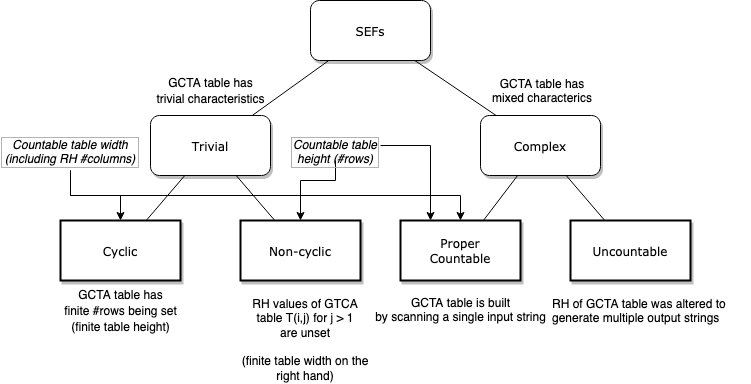
\includegraphics[width=\linewidth]{appendix/CategoriesOfSEFs.png}
  \end{subfigure}
  \caption{Categories of SEFs}
  \label{fig:sefcat}
\end{figure}

Following SEF notation one can define an infinite binary string by combining multiple formulas. A new category, presented in the above figure, is called \textit{complex} and has not yet been discussed. Indeed, according to the proposed categorization a mixture of two trivial SEFs, the cyclic or non-cyclic strings, will produce a GCTA table inherently combining their characteristics. Let us provide an example for it.

\begin{table}[ht]
  \caption{Example of a proper countable GCTA table for complex $\bos(01)(0)\eos$}
  \centering
  \begin{tabular}{ |c|r|l| }
    \hline
    \# & LH                 & RH              \\
    \hline
    1  & $\bos(01)\eos$     & $\bos(0)\eos$   \\
    2  & $\bos(01)0\eos$    & $\bos1(0)1\eos$ \\
    3  & $\bos(01)00\eos$   & $\bos0\eos$     \\
    4  & $\bos(01)000\eos$  & $\bos0\eos$     \\
    5  & $\bos(01)0000\eos$ & $\bos0\eos$     \\
    .. & ..                 & ..              \\
    \hline
  \end{tabular}
  \label{Tab:ComplexGCTA}
\end{table}

Let $b=\bos(01)(0)\eos$ be a bi-infinite binary input string. After scanning it with GCTA one obtains a proper countable table (as illustrated in table \ref{Tab:ComplexGCTA}). The mixed properties here are that the width and height of the table placeholders is both countable and set. In particular, first lines (\textit{\#1 and \#2}) contain cyclic formulas which expand infinitely to the right\footnote{validate RH value $1(0)1$ at line \textit{\#2} for yourself}. Now next lines do not have values of the RH placeholders set starting with the column index $j > 0, j \in J, J \subset \integers$. Although $b=\bos(01)(0)\eos$ consists of two trivial cyclic strings, it is not trivial by itself. In the sense of proposed categorization, GCTA table characteristics observed are similar to both cyclic string $\bos(01)\eos$ in the first lines and non-cyclic string $\bos[1+]\eos$ for the rest.

\subsection{Context argument}

We start by scanning a bi-infinite non-trivial binary string $b = \bos(0)[1+]\eos $ and producing a proper GCTA table $T(i,j)$.

The left-hand of $T(i,j),  \forall j < 0$ will contain all left-infinite strings  observed during scanning of $b$ by construction. Based on the characteristics of non-trivial infinite binary strings the right-hand of $T(i,j),i \in I, I \subset \nat, j \in J, J \subset \integers$ will exhibit both trivial non-cyclic and cyclic characteristics. This means we will have at least one cyclic-like bi-infinite entry $\bos(0)1\eos$ obtained by scanning $\bos(0)\eos$ resulting from zero-padding of $b$ on the left (see line \#1 in table \ref{Tab:GCGA})).

The other part of $b = \bos..[1+]\eos $ generates a unique countable sequence, which is continuously appended on the right. Scanning bits of this infinite sequence results in a list of countably many prefixes on the left-hand of $T(i,j),  \forall j < 0$. The corresponding right-hand entries will be unset for all $\forall j > 0, i > 1$  in $T(i,j)$.


\begin{table}[ht]
  \caption{Initial configuration with proper GCTA table for complex $\bos(0)[1+]\eos$}
  \centering
  \begin{tabular}{ |c|r|l| }
    \hline
    \# & LH                      & RH             \\
    \hline
    1  & $\bos(0)\eos$           & $\bos(0)1\eos$ \\
    2  & $\bos(0)1\eos$          & $\bos0\eos$    \\
    3  & $\bos(0)10\eos$         & $\bos1\eos$    \\
    4  & $\bos(0)101\eos$        & $\bos1\eos$    \\
    5  & $\bos(0)1011\eos$       & $\bos0\eos$    \\
    6  & $\bos(0)10110\eos$      & $\bos1\eos$    \\
    7  & $\bos(0)101101\eos$     & $\bos1\eos$    \\
    8  & $\bos(0)1011011\eos$    & $\bos1\eos$    \\
    9  & $\bos(0)10110111\eos$   & $\bos0\eos$    \\
    10 & $\bos(0)101101110\eos$  & $\bos0\eos$    \\
    11 & $\bos(0)1011011100\eos$ & $\bos1\eos$    \\
    .. & ..                      & ..             \\
    \hline
  \end{tabular}
  \label{Tab:GCGA}
\end{table}

Note that at this point string lists on both left-hand $LH = {T(i,j): j < 0}$ and right-hand $RH = {T(i,j): j >= 0}$ share the same cardinality due to line-by-line\footnote{one-to-one and onto} correspondence. We will denote them as $|LH|$ and $|RH|$ respectively. Both are countable $|LH| = |RH| = |\nat|$.

We will refer to the above setup as an \textit{initial configuration} and use it as a starting point for some proofs below\footnote{many similar configurations are equally acceptable for our purposes}. Will also refer to Cantor's slash argument\footnote{for example, as offered in comprehensive introductory overviews into the concept such as \cite{penrose2007road}} as well as employ some well accepted notations from the theory of smaller and Large Cardinals\footnote{namely, $\aleph_0=|\nat|$ - also see next section for more detailed recap of existing results and notations}.

For convenience, we will refer to the output result of GCGA as a table $T^\prime(i^\prime,j^\prime) = GCGA(b, T(i,j))$ containing those accessible strings or equivalently as to the left-hand $LH^\prime = T^\prime(i^\prime,j^\prime), j^\prime < 0$ and the right hand $RH^\prime = T^\prime(i^\prime,j^\prime), j^\prime \geq 0$. Like that we will treat $T^\prime(i^\prime,j^\prime)$ as a cursor function and sometimes abuse or omit the index notation by meaning enumeration in a wider sense as $\forall i^\prime \in I^\prime, I^\prime \supseteq \nat$ and $\forall j^\prime \in J^\prime, J^\prime \supseteq \nat$ when discussing $T^\prime(i^\prime,j^\prime)$.

Now let us describe how GCGA can act on the initial configuration by assigning values to the previously unset placeholders on the right-hand $RH = {T(i,j): j >= 0}$ in order to produce unobserved state and generate the multitude of output strings (\textit{GCGA steps}):

\begin{enumerate}
  \item create a reference of $T(i,j)$ from the initial configuration as $T^\prime(i^\prime,j^\prime)$ which is both relative to original $T(i,j)$\footnote{acts as copy of $T(i,j)$} and otherwise contains the same values except that it can also be modified or expanded with new placeholders at need so that all indexes are respectively relabeled;
  \item start moving the cursor in the top-down direction from the point closer the top-middle of the $T^\prime(i^\prime,j^\prime)$ by examining values at $i^\prime = 0, j^\prime = 1$ on the right hand of the proper table;
  \item continue to increment access index $i^\prime$ until one can find the placeholder for the state value that has not yet been set at some $i^\prime \geq 0, j^\prime \geq 1$\footnote{optionally and in case of other input strings, one can also increment j up to some finite size of the SEF formula in the state (if desired) and look further on the right for the unset placeholders};
  \item if the values for $j^\prime > 0$ are unset, this means that the prefix on the same counter-part line on the left has been observed only once. Then one can label this location as \textit{suitable for modification};
  \item next, GCGA can be run similar to GCTA steps to output the result with some difference in conditional logic as explained below;
  \item continue with generation on every line by switching between context prefixes
  \item if the the line at index $i^\prime$ can be marked as \textit{suitable for modification}, then:
        \begin{enumerate}
          \item mark corresponding prefix in the LH of $T^\prime(i^\prime,j^\prime), j^\prime<0$ as copied, so that only the finite reference is stored\footnote{we interpret output with such finite separator reference as "multi-lined"}
          \item keep expanding $T^\prime(i^\prime,j^\prime)$ with copies of the marked string including the unset placeholder on the right, preparing them for the modification at the next steps
          \item continue to run the necessary number of iterations for that $i^\prime$ so that one can cover the entire space of yet unset placeholders on the right-hand of $T^\prime(i^\prime,j^\prime), j^\prime>0$ by some countable index mapping $k \rightarrow (i^\prime,j^\prime), k \in K, K \subset \nat$
          \item once you run as many finite iterations of SEFs enumeration for each index pair $(i, j)$  as required by the above one-to-one and onto mapping, append newly obtained binary values to the unset placeholders on the right of $T^\prime(i^\prime,j^\prime), j^\prime > 0$
          \item optionally, generate an output string each time the new placeholder is appended
          \item update $(i^\prime,j^\prime)$ for the next iteration of the cover on the same line either by remembering values or computing them from the cover mapping
          \item continue to loop over the covering map $k \rightarrow (i^\prime,j^\prime)$ to repeat the above sub-process from step 3 as many times as necessary\footnote{up to countably many times} or until you have reached the output values desired by the access or a cursor function
        \end{enumerate}
\end{enumerate}

Keep in mind, that every appending (generation) happening in the steps 7(c) and 7(d) of \textit{GCGA steps} over previously unset values is interpreted as access (generation) of a new output infinite binary string which continues to expand with the new unobserved part of the prefix \footnote{due to construction of the algorithm}. Unless designed, the described algorithm will never terminate for the specific input string $b = \bos(0)[1+]\eos$. In fact, this is not necessary for our purposes as it is enough to show that:
\begin{itemize}
  \item the above description of GCGA algorithm generates new unique strings from the point of view of the particular "fork" or branch starting at some $(i^\prime,j^\prime)$
  \item as well as provides the ability to access the necessary values at the exact "fork" or branch observed after the given context in $LH$
\end{itemize}

It is easy to see that GCGA can be further modified to print out only desired or finite parts of the output. Recall, that we refer to such output strings as algorithmically reachable by a cursor.

We can observe that after applying GCGA to the $T(i,j)$, the table will not be proper anymore in a sense that the left-hand $LH^\prime$ contains duplicates, which are still unique strings only if considered jointly with their right-hand counter-parts in $RH^\prime$ list.

It is important to stress the following fact again - the property that makes every new string listed in the table $T^\prime(i^\prime,j^\prime)$ unique is the peculiar design of GCGA, which goes beyond counting\footnote{in a sense of recursive construction of natural numbers $\nat = \{x_{i+1} = x_{i} + 1\}, \forall i \in I$} and is simply a special way of accessing every traversable object that can be output by the algorithm with or without given context in $LH$.


We have reached the point when we know how $T^\prime(i^\prime,j^\prime)$ can work by applying GCGA to $T(i,j)$ values. It is still not clear if left and right "table halves" when accessed via the respective cursor functions $T(i,j)$ and $T^\prime(i^\prime,j^\prime)$ can result in producing the output of the same left and right cardinality $|LH| \stackrel{?}{=} |RH^\prime|$ or alternatively can access parts of one or more unique bi-infinite binary strings which we can show to be unequal.


\begin{theorem}
  Let $T^\prime(i^\prime,j^\prime) = GCGA(b, T(i,j))$, where both $T^\prime(i^\prime,j^\prime)$ and $T(i,j)$ are cursor functions as well as $T(i,j)$ is a proper table over input bi-infinite binary string $b$ and $b$ is proper countable. Cardinality of $|LH| < |RH^\prime|$ when accessed via $T(i,j)$ and $T^\prime(i^\prime,j^\prime)$ from input $b$ respectively.
\end{theorem}

\begin{proof}The above statement  $|LH| < |RH^\prime|$ can have a meaningful answer only when we recall that $T^\prime(i^\prime,j^\prime)$ tries not just to access but also to generate new elements in the sense of the algorithm application explained above in \textit{GCGA steps}. Let $b = \bos(0)[1+]\eos$ or any other proper countable input string. Proceed with initial configuration and apply GCGA steps to $T(i,j)$ proper table constructed with GCTA. We can produce any arbitrary or specifically requested output range through means of the cursor $T^\prime(i^\prime,j^\prime)$.

  Now let us show that the resulting output of applying GCGA will fall into the category of the proper uncountable strings. We can point out the exact difference in the end result of the traversing process up to specific index. In order to do so, choose any nearest $(i^\prime,j^\prime)$ index pair suitable for modification (\textit{GCGA step 7.c}). Observe that $j^\prime > 0$ meaning the cursor is pointing at the yet unset placeholder in both $T(i^\prime,j^\prime)$ and $T^\prime(i^\prime,j^\prime)$. Select the row $i^\prime$ from $T(i,j)$ table without any unset values as a left-infinite string $a := (T(i^\prime,j), \forall j < j^\prime)$. Iterate further through GCGA steps to pick next suitable value $v \in \{0, 1\}$ from the generation scheme (or pattern, such as "[1+]"). Assign that value at the cursor $T^\prime(i^\prime,j^\prime) := v$. Select the row from $T^\prime(i^\prime,j^\prime), \forall j^\prime$ without any unset values as a left-infinite string $a^\prime$. Observe that $a^\prime \neq a$ and is different up to a single placeholder that is still unset in $T(i^\prime,j^\prime)$. Then notice that string $a$ is also a prefix of $a^\prime$ as in $a = ".., a^\prime[j^\prime-2], a^\prime[j^\prime-1]"$. If $a^\prime \notin T$ table, then $|LH| < |RH^\prime|$. Indeed, assume the opposite that $a^\prime \in T$. By design of GCTA the $T(i,j)$ table is constructed as proper, meaning that $T(i^\prime,j^\prime)$ can have multiple states assigned for the prefix of $a$ in $RH$ iff the prefix of the left-infinite string $a$ is observed in $b$ multiple times. The latter is not the case. Neither prefix of $a$ nor $a$ is observed in $b$ more than once, hence $a^\prime \notin T$.

  This new string $a^\prime$ has been just appended to $T^\prime$ table by GCGA, so that $i^\prime := i + 1$. We can continue to generate similar new and unique strings and access them by means of the $T^\prime(i^\prime,j^\prime)$ cursor an exact and finite number of times\footnote{by design and implementation of GCGA}, until we switch to the next index suitable for modification. However, that means that $RH^\prime$ is strictly uncountable and $|LH| < |RH^\prime|$. \end{proof}

One should avoid confusions in interpreting the results stated in the \textit{Theorem 10}. We have shown that one can use GCGA \footnote{or similar schemes} to achieve algorithmic accessibility when it comes to handling larger objects arranged from infinite binary strings. Such schemes can be used to construct and access objects like $RH^\prime$ demonstrating to have the property of strictly greater cardinality over $|\nat|$. However, if we run GCGA implementation on a deterministic TM any produced output will be naturally of the same countable cardinality, just as the one of GCTA \footnote{with the only difference in the printed-out values}. We are again in need of tools that can help us operate with such objects of greater uncountable cardinality more intuitively.

\subsection{Uncountable cardinalities}

In the previous section (see - \textit{Theorem 10}) we have indicated yet another way\footnote{next to natural numbers as well as transfinite cardinal and ordinal numerals - read further for more detailed explanation} for how to count at infinity or expand upon large objects such as lists of infinite binary strings. Next, we will reference and introduce some more of notation to be able to discuss previously known theory and its results. Our intention is to better understand potential consequences of such presumably novel "counting" technique.

We begin by following into the original line of thinking as offered by George Cantor. Cantor introduces a theory for transfinite numerals called ordinals and defines their cardinalities. He also famously introduces the Cantor's diagonal or slashing argument\footnote{Further we will refer to Cantor's diagonal argument simply as \textit{slashing}}. The idea behind slashing is to compare cardinalities of rather large objects such as infinite lists of items by employing the bijective mapping\footnote{An instructive overview of these and other ideas by Cantor\cite{cantor1915contributions} for matching cardinalities (starting with $|\rationals| = |\nat|$) has been cleverly outlined in "Hilbert's Hotel" by Gamow\cite{gamow1988one}, p.17.}. 

Bijective mapping of objects is such a central tool to the discussion of cardinality (in the proposed set theory by Cantor and beyond) that we want to state it even more formally as a principle.
\begin{principle}[Principle of one-to-one correspondence]\label{principle_1to1_cor}
  Objects have the same cardinality if and only if their elements are in one-to-one correspondence. 
\end{principle}
One-to-one correspondence between objects is usually proved by showing the existence of the respective bijective mappings or, equivalently, functions which are both one-to-one and onto\footnote{Also see the set theoretical definitions for bijective functions as discussed, for example, in\cite{goldrei1996classic, kunen1980set, jech2003set}}.

Again, this principle turned out to be very insightful and helped to make sense out of many less-intuitive situations when objects were looked upon much more restrictively - for example, only from the perspective of trivial counting. Let us recap on that.

Recall that counting procedure provides us with the set of natural numbers $\nat = \{1, 2, 3..\}$. Any taken subset of natural numbers $ X \subset \nat$ will be always limited by some largest number at the very end of such subsequence $X$, meaning that the cardinality of such subset is finite $|X| < |\nat|$. However since the sequence of the natural numbers $\nat$ by itself is always constantly appended with a new number which will be an increment of the previously seen largest number, we say that the cardinality of natural numbers is actually infinite and corresponds to the countable form of infinity. This can be captured by assuming the existence of some transfinite limit $\omega_{0}$\footnote{$\infty$ sign was suggested to be replaced by Cantor with $\omega$ which is a less confusing notation\cite{cantor1915contributions}}. This limit $\omega_{0}$ is strictly greater than any natural number\footnote{which is also a definition of any transfinite numeral - see \cite{jech2003set} for much better introduction into ordinals} and will be a first transfinite number such that if $X^\prime \subseteq \nat \cup \{\omega_{0}\} $, then we say such subset has a first infinite or countable cardinality similar to that of natural numbers. Cardinality of sets that include ordinal limits is notated with aleph letters. For example, for the inclusion of the first ordinal limit $\omega_{0}$ we use $\aleph_{0}$ and say $ \aleph_{0} = |X^\prime| = |\nat|$. The idea of transfinite numbers gets further developed by introducing the theory of \textit{ordinal numbers}\cite{cantor1915contributions}.

A set of natural numbers consist of elements which can be counted and hence \textit{well-ordered}. Counting provides order-preserving bijection for well-ordered sets by labeling\footnote{and simply agreeing that the order of some elements is greater than the others}. Each cardinal number can be related to some limit ordinal of the underlying set. For example, for natural numbers\footnote{by re-ordering a set we can assign it a new order type} that would be a first order type $\omega_{0}$\footnote{mind the index at omega for convenient mapping with alephs further on}. Thus we say that any of the ordinals starting with $\omega_{0}$ in the well-ordered sequence $\omega_{0},\ \omega_{0} + 1,\ \omega_{0} + 2,\ ..  $ will be strictly greater than any natural number. All $\omega_{0}$ ordinals such as $\{\omega_{0},\ \omega_{0} + 1,\ \omega_{0} + 2,\ ..\}$ correspond to the first transfinite cardinal $\aleph_{0}$. Similar association is true for the next biggest transfinite cardinal $\aleph_{1}$, to which all $\omega_{1}$ ordinals such as $\{\omega_{1},\ \omega_{1} + 1,\ \omega_{1} + 2,\ ..\}$ can be mapped to as many to one\footnote{in most frameworks like Zermelo–Fraenkel (ZF) set theory this usually requires an \textit{Axiom of replacement}}. We say that $\aleph_{1}$ is a first transfinite cardinal for the infinite set with uncountable cardinality.

Although $\omega_{0}$ and $\omega_{0} + 1$ have different respective order types, they do not add more to the original cardinality $\aleph_{0}$ of the corresponding set $\nat$\footnote{keep in mind that re-ordering the set does not change its cardinality, even in case of transfinite sets}. To reiterate over the idea of cardinalities of ordinal transfinite numerals again - indeed, if ordered set $\nat \cup \{\omega_{0}\} = \{0, 1, 2, 3, .., \omega_{0}\}$, then the cardinality $|\nat \cup \{\omega_{0}\}|$ is still the same as $|\nat| = \aleph_{0}$.

Recall that ordinals are defined as order preserving sets, but transitive addition in ordinal arithmetic is not commutative\footnote{contrary to the definitions of ordinal arithmetic and in case if natural ordinal arithmetic is applied, one can achieve $1 + \omega_{0} = \omega_{0} + 1$ }. One can still have the well-ordering in form of right-side addition as in $\omega_{0} < \omega_{0} + 1$, even though it is not the same for left-side addition when $1 + \omega_{0} = \omega_{0}$. This means that applying ordinal arithmetic will not result in order preserving bijections between $\nat \cup \{\omega_{0}\}$ and $\{\omega_{0}\} \cup \nat$. Namely, the later will have order type $1 + \omega_{0} = \omega_{0}$, based on the bijection $\{\omega_{0} \rightarrow 0, i \rightarrow i + 1 : \forall i \in \nat \}$, and hence $1 + \omega_{0} < \omega_{0} + 1$.

Other interesting insights that we want to recap are based on the concept of powerset. This concept is a helpful example of yet another way to count things at infinity (next to transfinite ordinals). The concept itself is as following, if $X$ is a set of items, then a set $\pset(X)$ consists of all subsets of set $X$ and is called a \textit{powerset} of $X$.

Numbers can be constructed from sets. For example, applying only empty set one can show how to construct natural numbers \cite{penrose2007road}. The process of recursive application of \textit{powerset} to sets with cardinalities of $\aleph_0$ and larger is called \textit{transfinite exponentiation}. It can be also used to construct \textit{ordinals} from sets\footnote{for other than Cantor ordinals, please check von Neumann ordinals with an alternative proper-class construct: "each ordinal is the well-ordered set of all smaller ordinals"}. Such sets are referred to as \textit{omega sets}\footnote{mind the $\omega$ letter we have used earlier} of well-ordered numerals and can be used to show how greater orders of infinity (beyond countable) can be set up\footnote{ultimately by stating the existence of transfinite numerals as we have done earlier, see - \textit{"The Transfinite Ordinals and Cantor’s Mature Theory. In: Labyrinth of Thought"}\cite{ferreiros2008labyrinth}, pp. 257-296 as well as \cite{kanamori1996mathematical}}.

However, one has to be careful when working with such concepts as \textit{set of sets}. It has been proven to be unexpectedly complex and may easily lead to paradoxes\footnote{For example - \textit{Russell's paradox}} if no special considerations are put in place\footnote{For instance - the requirement to operate within certain logical framework which relies on axiomatic systems such as ZF set theory}. Whenever possible we will replace the notion of \textit{set of sets} either by considering \textit{lists of items}, where items are more concrete objects than sets such as binary strings or by simply looking at classes of numerals\footnote{Meaning that we try to implicitly employ the proper-class construct as proposed by ZF everywhere in our discussion}.

The powerset concept is used in another important result called Cantor's Theorem \footnote{see \cite{jech2003set} and for conceptual proof outline refer to \cite{penrose2007road}}:

\begin{theorem}If $|X| = \alpha$, then $|\pset(X)| = 2^\alpha$ and $\alpha < 2^\alpha$, where $2^\alpha$ is the total number of subsets of any set such as $X$.\end{theorem}

As a consequence one can state\footnote{Alternatively, one will rely on the proof using Cantor's diagonal argument\cite{penrose2007road} applied to the list of all binary strings} the existence of strictly greater cardinality $\aleph_{0} < 2^{\aleph_{0}}$. An assumption that $\aleph_{1} \stackrel{?}{=} 2^{\aleph_{0}}$ is equivalent to the \textit{continuum hypothesis}\footnote{Assuming the axiom of choice, there is the smallest cardinal number $\aleph_{1}$ greater than $\aleph_{0}$, and the \textit{continuum hypothesis} is in turn equivalent to the equality $\aleph_{1} = 2^{\aleph_{0}}$\cite{goldrei1996classic}.}, which needs more explanation.

We define the cardinality of real numbers as $\cont = |\reals|$. Cantor gave two proofs that the cardinality of the set of integers is strictly smaller than that of the set of real numbers $\aleph_{0} < \cont$\footnote{Cantor's first uncountability proof and Cantor's slashing}. However, those proofs provided no indication to which extent or how far does the difference of cardinality in $\aleph_{0} < \cont$ goes, so Cantor has proposed the continuum hypothesis (CH)\footnote{see \cite{jech2003set, herrlich2006ac} as well as \cite{enwiki:1062726958} for more informal but comprehensive covering} as a possible solution to this question. The CH states that there exists no set $S$ for which $ \aleph_{0} < |S| < \cont$\footnote{which is a weaker version of the CH formulation}.

\subsection{Formal SEF languages}

So far we have provided a number of definitions to describe infinite binary strings. Good news is that our discussion and results are not based on dealing with highly abstract sets\footnote{and equally large, such as \textit{von Neumann universe} in ZFC} yet, but rather with concrete objects like lists of binary strings\footnote{residing and computable within the realm of theoretical computer science}. This means we did not rely much on any foundational framework\footnote{such as ZFC}, so the results in \textit{Theorem 10} are mostly independent. Unfortunately at this point such results are still not formal enough to explain what exactly do we mean by \textit{uncountability} or how to interpret our claims about cardinality of inspected objects. Instead of moving forward with developing a complete theory of infinite binary strings from scratch\footnote{in terms of mathematical logic} by doing further build-up on presented GCGA concept, we intend to harden and refine our definitions referencing something well-known. We will do so by obtaining an exact explanation based on already existing results in classic set theory\footnote{which we have most briefly recapped and referenced in the previous section - also see \cite{goldrei1996classic}} and theoretical computer science\cite{Sipser05introcompther}.

With such motivation in mind, this subsection will focus on refining definitions of SEFs as formal languages\footnote{following Chomsky hierarchy}. Next subsection will describe an algorithm that we will refer to as \textit{continuum access scheme} (CAS) and benefit from the definitions.

Recall that in computer science\cite{Sipser05introcompther} a formal language is defined over some alphabet. An alphabet is usually a finite set or list of symbols or sometimes strings. For example in both cases, $\Sigma=\{0,1\}$ or $\Sigma=\{ab,ba,c\}$ are alphabets.

\begin{definition}
  If $\Sigma$ is a finite set of strings called alphabet, then $\Sigma^*$ is an infinite list of all possible concatenations over those strings, s.t. $|\Sigma^*| = \aleph_0$.
\end{definition}

The star symbol notation used in $\Sigma^*$ is called Kleene-closure of $\Sigma$. Alternatively, $\Sigma^*$ is said to be closed under string concatenations including the empty string $\epsilon$\footnote{a zero length string, similar to the empty set element}.

A formal language consists of \textit{words} whose letters are taken from an alphabet and are \textit{well-formed} according to some specific set of rules.

\begin{definition}
  If $\Sigma$ is a finite alphabet, then a \textit{formal language} $L$ over an alphabet $\Sigma$ is defined as a set $L := \{ w\ is\ valid : \forall w \in \Sigma^* \}$, where each word $w$ is a \textit{well-formed} or \textit{valid} expression of $L$.
\end{definition}

Words of formal languages can be also referred to as expressions or formulas. Now we want to take a closer look at what does the {well-formed expression} means or the notion of formula validity for SEFs by summarizing what has been discussed about SEFs so far as a set of rules.

\begin{definition}
  A formula $\phi$ is a valid String Enumeration Formula iff all of the following is true:

  \begin{enumerate}
    \item $\phi$ is an input-free program generating an infinite binary string as an output in countable time\footnote{meaning that number of output characters or the cardinality of the output is never greater than $\aleph_0$ - also see \textit{Definition 11}}
    \item formula has always a finite length $|\phi| = m: m \in \nat$ unless specified otherwise\footnote{one can explicitly specify countable length for $\phi, |\phi| = \omega_0: \omega_0 > n, \forall n \in \nat$}
    \item replicator syntax is a balanced pair of round brackets such that number of balanced bracket pairs is finite $|\phi|_{(} = |\phi|_{)} = n: n \geq 0, n \in \nat \cup \{0\}$
    \item round brackets can be nested which is interpreted as recursive replicator calls
    \item a replicator can not be defined over an empty string
  \end{enumerate}
\end{definition}

Given the notion of SEF validity we can define a \textit{didactic} procedure as an algorithm accepting only valid input expressions. This also allows stating the definition of a formal language for SEFs.

\begin{definition}A Formal String Enumeration Formula language or \textit{SEF language} is a formal language constructed from syntactically valid formulas over alphabet $\Sigma$ as $L_{SEF} := \Delta(\Sigma^*)$, where $\Delta$\footnote{do not confuse with $\Delta_0$ formulas\cite{jech2003set} of first order logic} is a validation procedure or \textit{didactic} that can recognize only well-formed expressions of $L_{SEF}$. $\Sigma := V \cup \gamma$ is a union between set $V$ of vocabulary symbols and set $\gamma$ of syntactical symbols (syntax).\end{definition}

One can state an equivalent definition.

\begin{definition}$L_{SEF}$ is a \textit{SEF language} constructable from a tuple $(\Sigma, \Delta)$ iff $\Delta \subset \Sigma^*$ s.t. all formulas in $\Delta$ must be both syntactically valid and computable as SEFs.\end{definition}

Note that for most purposes formal languages are defined over finite alphabet. The same is with SEF languages unless specifically considered.

\begin{definition}If $L_{SEF} := (\Sigma, \Delta)$ is a SEF language and $\exists k \in \nat: |\Sigma| \leq k$, then we say that $L_{SEF}$ has an alphabet with finite cardinality $k$.\end{definition}

This is different from the cardinality of the language which is a set of all valid formulas.

\begin{definition}If $L_{SEF} := (\Sigma, \Delta)$ is a SEF language then the cardinality of the language is the same as $|\Delta|$.\end{definition}

Finally, we say that the language is finite if it can recognize strings of finite length.

\begin{definition}If $L_{SEF} := (\Sigma, \Delta)$ is a SEF language and each formula of the language is finite $\forall \phi \in \Delta: |\phi| \leq n, n \in \nat$ then we say that $L_{SEF}$ is a finite language.\end{definition}

\begin{theorem}
  If $L_{SEF} := (\Sigma, \Delta)$ is a finite SEF language then $L_{SEF}$ is also a regular language.
\end{theorem}
\begin{proof}
  Recall the result from \cite{Sipser05introcompther} that every formal language is a regular language iff it can be recognized using a regular expression. Observe that regular expressions themselves form a regular language or can be parsed by a regular expression. Since every SEF expression can be reduced to a regular expression by mapping replicator syntax to a Kleene-closure, it means that there exists a regular expression to parse SEFs.
\end{proof}

Obviously, even if both the cardinality of the alphabet\footnote{i.e. $| V \cup \gamma| \geq \aleph_{0}$} and the cardinality of the SEF language itself\footnote{language contains formulas of countable length} is infinite, it can be still restricted by some greater cardinality unless shown or defined otherwise.

Please note that so far we have been working only with finite SEF languages and will continue to do so. For example, $L_{SEF} := (\Sigma, \Delta) = (\{0,1\} \cup \{{(}, {)}, {:}\}, \Delta)$ is a finite SEF language equipped with round brackets as replicator symbols and colon for access symbol and $\forall \phi \in \Delta: |\phi| \leq n, n \in \nat$. If needs be, the extended version of the syntaxes may include square brackets for binary conversion of in-line decimals as well as plus and star generating short-hands for enumeration scanning.

Next we would need one more definition to count how many times one sub-string can occur in another string.

\begin{definition}Given $L_{SEF}$ is a SEF language and $\exists z,s: z,s \in \Delta$ are valid strings in that language, such that one string can occur in another one at least once, i.e. $z \in s$. This fact is noted as $|s|_{z}$ and is called cardinality of $z$ in $s$.\end{definition}

In case when we can count how many times one sub-string can occur in another string, then this is noted as $|s|_{z} = \lambda: \lambda \in \nat$.

\subsection{Continuum access scheme}\label{subsec_cas}

We base on the setting similar to the GCGA initial configuration. We start by scanning a string $b=\bos(0)[1+]\eos$ with a small difference in approach but without loss of generality. Instead of scanning bit by bit, we jump over the full binary representation from one integer $\bos(0)[1][2]\eos$ to the next one $\bos(0)[1][2][3]\eos$. Such scanning is marked as $b=\bos(0)[1*]\eos$. Like that all bits of each integer are concatenated at full for every string we add to $LH$ of the table (see fig. \ref{fig:continuuma}).

\begin{figure}[h!]
  \centering
  \begin{subfigure}[b]{0.9\linewidth}
    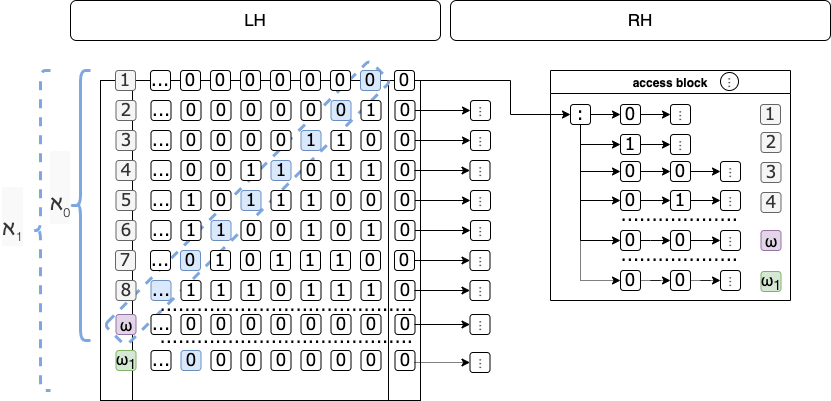
\includegraphics[width=\linewidth]{appendix/access-scheme.png}
  \end{subfigure}
  \caption{Continuum access scheme}
  \label{fig:continuuma}
\end{figure}

We also extend the SEF formula language of infinite binary string enumeration using a colon symbol. On the $RH$ of the table we have something called \textit{access block} labeled with three vertical dots. The expanded version of this block contains the access step noted with colon symbol. Keep in mind that the access block is recursive. For example, a string formula that indicates some instance of algorithmic access from the $LH$ context with the span into the $RH$ is designated as $\bos(0)[1]{:}01{:}010({:}0)\eos$, where the string replicator on the very right end $\bos..({:}0)\eos$ represents a continuous access action into the $RH$. When one needs to compute such an infinite binary string formula, one can imagine a computation process by expanding each replicator without stop. The replicator with the access colon symbol means continuous recursive access with ever expanding context on the left hand of each colon. This schematic representation describes nothing else but the recursive application of the GCGA and can be seen as yet another generalization step through the employment of the recursive definition.

On one hand, we don't necessarily need to restrict number of times when the colon symbol appears in such extended SEF notation. Indeed, such cases can be called an infinite algorithmic access scheme or simply \textit{continuum access scheme}. On the other hand, if we would prefer to restrict number of occurrences for the colon symbol by some finite limit, that should be possible as well.

Now let us consider another simplification with the finer subcase of applying continuum access scheme (see fig. \ref{fig:continuuma}) but only a limited number of times.

\begin{definition}If $L_{SEF} := (V \cup \gamma, \Delta_\delta)$ is a finite SEF language, which syntax is equipped with a colon as an access symbol and any formula in its didactic set $\Delta_\delta$ contains colon symbol but only limited number of times, then we say that language $L_{SEF}$ has some finite depth of $\delta$. Specifically, $\exists \delta \in \nat, \forall s \in \Delta : |s|_{{:}} \leq \delta$.\end{definition}

Access schema for languages with finite depth can be imagined as similar to fig.\ref{fig:continuuma} but without having an infinite recursion call inside the access block\footnote{a block with the three vertical dots symbol}. Number of calls becomes limited by counting. We are particularly interested in this case as we can show not only that there is no bijection between LH and RH parts of the corresponding computationally expanded GCGA table\footnote{by applying result from \textit{Theorem 10}}, but specifically to extend and pin-point the relationship between LH and RH parts.

Let $L_{SEF} := (V \cup \gamma, \Delta_1)$ be a finite SEF language with a binary vocabulary $V := \{0,1\}$, typical syntax $\gamma := \{{(}, {)}, {:}\}$ and didactic with a single access depth, s.t. $\forall s \in \Delta : |s|_{{:}} = 1$. Consider a proper table with cursor $T(i,j)$ obtained by scanning a proper countable bi-infinite input binary string $b$ and a cursor function $T^\prime(i^\prime,j^\prime)$ such that $T^\prime(i^\prime,j^\prime) = GCGA(b, T(i,j))$ which will allow algorithmic access as exposed in \textit{Theorem 10}. For instance, if $\exists i^\prime,j^\prime: i^\prime \in I^\prime$ and $j^\prime \in J^\prime$ are some indexes and there is a formula $f := \bos(0)1{:}01\eos$ corresponding to $i^\prime \in I^\prime$, then the sub-string before the colon (acting as an access symbol) will correspond to the context of the expanded string accessed via cursor function $T^\prime(i^\prime,j^\prime): \forall j^\prime < 0, j^\prime \in J^\prime$ and will be equal to $\bos(0)1\eos$. While the part after the colon corresponds to the value-state of the expanded string from $T^\prime(i^\prime,j^\prime): \forall j^\prime > 0, j^\prime \in J^\prime$ and will be equal to $\bos01\eos$.

The above approach is similar for finite languages of greater depth. For example, in case of $L_{SEF} := (V \cup \gamma, \Delta_2)$ if there is a formula $f := \bos(0)1{:}01{:}1\eos$, then the whole sub-string before the second occurrence of the colon symbol will correspond to the context when the second access is evaluated. However, for greater clarity we replace multiple-prime notation with depth index. This applies to cursor functions $T_\delta(i,j)$, so that

\begin{align*}
  if\:\delta = 1{:} & \quad T_{1}(i,j) := T^\prime(i^\prime,j^\prime)                            \\
  if\:\delta = 2{:} & \quad T_{2}(i,j) := T^{\prime \prime}(i^{\prime \prime},j^{\prime \prime}) \\
  ... {   }         &
\end{align*}

and so on. Also further we assume that depending on the context the cursor indexes $i, j$ are remapped from their index supersets accordingly. For example, $j^\prime \in J^\prime$  is always re-mapped from $j^{\prime \prime} \in J^{\prime \prime}$\footnote{projected or pulled from the superset - for example, this can be implemented via Levy collapse of cardinals\cite{jech2003set}; we also discuss implementation of CAS in later subsections} via $\alpha: J^{\prime \prime} \to J^\prime$ based on depth and occurrence of the access symbol and given that $J^\prime \subseteq J^{\prime \prime}$. Such mapping is equivalently rewritten as $\alpha: J_2 \to J_1$, where $j_1 \in J_1, j_2 \in J_2, J_1 \subseteq J_2$. The same is true for $LH^\prime$ and $RH^{\prime \prime}$ being rewritten as $LH_1$ and $RH_2$.

\begin{theorem}Let $L_{SEF} := (\{0,1\} \cup \{{(}, {)}, {:}\}, \Delta_\delta)$ be a finite SEF language with a binary vocabulary, typical syntax and didactic with a finite depth $\delta \in \nat$. If a cursor function $T_\delta(i,j)$ implements continuum access schema for $L_{SEF}$ limited by some finite $\delta \in \nat$ for every formula in didactic $\Delta_\delta$, then for every algorithmically accessed value-state sub-string $\forall \nu_\delta \in RH_{\delta+1}: \nu_\delta := T_{\delta+1}(i,j): \forall j > 0, j \in J_{\delta+1}, i \in I_{\delta+1}$ given context $\phi_\delta \in LH_\delta: \phi_\delta := T_\delta(i,j): \forall j < 0, j \in J_\delta, i \in I_\delta$ there exists surjection

  \begin{align*}
    \rho_\delta \colon RH_{\delta+1} & \to LH_\delta       \\
    \nu_\delta                       & \mapsto \phi_\delta
  \end{align*}

  such that at least for $\delta = 0: |LH_\delta| < |RH_{\delta+1}|$ and $|RH_{\delta+1}| \leq |\pset(LH_\delta)|$, where $\pset(X)$ is a powerset of $X$.\end{theorem}

\begin{proof}The theorem is proven by following the construction of the continuum access schema.

  A finite case for the existence of the surjection $\rho \colon RH_1 \to LH$ is trivial. It is enough to show that $\rho: \nu \mapsto \phi$, where $\forall n \in \nat, m \in \{1, .., 2^n\}: \nu = \bos[m]\eos, \phi = \bos[n]\eos$, which is the case for $T_1(i,j)$ table with any finite number of $i \leq 2^n$ lines. Given that the $|\pset(X)| = 2^{|X|}$ if $X$ is a finite set, then the existence of the surjection $\rho \colon RH_1 \to LH$ is satisfied for $LH$ of $T(i,j)$ and $RH_1$ of $T_1(i,j)$.

  For the infinite case we need to consider $|LH| \geq \aleph_0$. This can be achieved by slashing $LH$ as shown on fig.\ref{fig:continuuma}, then adding an inverted diagonal as new string labeled $\omega$ to $LH := LH \cup \{\omega\} $ and extending $RH$ with the link to access block accordingly. So far we have not commented on how the $RH$ part of $T(i,j)$ is expanded. Continuum access is implemented based on Theorem 10 result by recursively applying GCGA as in $T_{\delta+1}(i,j) := GCGA(b, T_\delta(i,j))$, where input $b$ can be ignored after initial application. The role of $RH_{\delta+1}$ extension is performed by the access block, so that each entry in the access block is interpreted as value-state sub-string before the next iteration down the recursive call. Like that value-state of the previous iteration of the access call becomes appended (concatenated) to the new context of the next access call.

  Note that given $L_{SEF}$ and for all countably and recursively extendable cases of $LH_\delta: \delta \in \nat$ the access block always represents an infinite access scheme to all possible infinite binary strings, the cardinality of which by Cantor's theorem equals to $2^{\aleph_0}$ due to existing bijection between the set of all infinite binary strings and continuum of real numbers $\reals$. The same theorem states $2^{\aleph_0} = |\pset(\aleph_0)|$\cite{jech2003set}.

  Both for finite and infinitely recursive access blocks we still rely on the algorithmic access as a possible selective reference to higher value-states of $\delta \geq 1$. Specifically, one can think of $RH_{\delta+1}$ values getting pulled down into $LH_{\delta}$ at need \footnote{only when provided with the specific context}.

  Now in our case, $L_{SEF}$ language is finite and $\delta \leq 1$. Since the access block recursion is called only finite number of times we can only state that the right-hand is not greater than cardinality of the continuum or $|RH_{\delta+1}| \leq |\pset(\aleph_0)|$

  Given that $|LH| = \aleph_0$ and using generalization of Theorem 10 by induction, one has $|LH_{\delta}| < |RH_{\delta+1}|$. This means there exists a surjection  $\rho_\delta \colon RH_{\delta+1} \to LH_\delta$, specifically such that $|LH_\delta| < |RH_{\delta+1}|$ and $|RH_{\delta+1}| \leq |\pset(LH_\delta)|$ at least for $\delta = 0$.\end{proof}

A valid concern would be to ask if such continuum access schema is computable on a general computer or an equivalent TM. The answer is \textit{no} and it follows from the following explanation. Indeed, from computer theoretical perspective this still means that not every infinite binary string can be accessed\footnote{see \textit{halting problem} for details} with existing computers. Another way to say the same is that \textit{every algebraic number is computable} or \textit{every transcendental number is incomputable}\footnote{every Chaitin's constant is the example of incomputable number - also see subsection \textit{Computability of SEF languages}}. Even if one would take a step back to assume the existence of some special-purpose formalism\footnote{uncommon enough, beyond general computer programs} that would permit efficient implementation of the algorithm\footnote{or rather a schema} for the described continuum access schema for all left-infinite countably extendable expansions of contexts in $LH_\delta: \delta \in \nat$ then most likely such algorithm is neither in RE nor in co-RE complexity class\footnote{this however should be more carefully reviewed for the $\omega$-regular languages and respective "$\omega$-RE" class if only such can be meaningfully defined for some extended version of Chomsky hierarchy}.

One can notice that once we have applied slashing to $LH$ (see fig.\ref{fig:continuuma}) as according to the explanation in the above proof, we can repeat the process to obtain $\omega_1$ string and produce an uncountable extension of $|LH| = \aleph_1$. Technically there is nothing stopping us from doing so at this point. Another peculiarity is that the proof of Theorem 12 was obtained only for the case of at least $\delta = 0$, without full generalization by induction. The reason behind this is a valid concern that we don't necessarily know yet how big is exactly the cardinality of the continuum $\cont = 2^{\aleph_0}$. In fact, besides highlighting such concern, the Theorem 12 does not provide any additional insights except already known results due to Cantor's work\cite{cantor1915contributions, kanamori1996mathematical, goldrei1996classic}. However, we did manage to provide an illustration of relation between cardinalities of $\aleph_0$, $\aleph_1$ and $2^{\aleph_0}$ in form of continuum access schema using infinite binary strings as well as the connection to the set theoretical axioms\footnote{ultimately, by building up on the result of Theorem 10 - so that uncountability concept is fully aligned with the original set theoretical notion by Cantor}.

\subsection{Uncountability of SEF languages}

On one hand we have looked at the definitions of formal SEF languages which have a finite alphabet and consist of countably many formulas of finite length. This aligns nicely with the well-known formalism in computer science theory such as regular languages. On the other hand, the motivation behind SEFs was to have an expression which produces an infinite binary string. But if we want to expand on our understanding of uncountability, we would need to look into extending the definition of formal SEF languages to be able to handle expressions of infinite length.

Let us revise some properties of the formulas in a finite SEF language $L_{SEF} := (\Sigma, \Delta)$. Each valid $\phi \in \Delta$ can be computed into some infinite binary string $b \in \cbin, |b| = \aleph_0$ to produce an output. In fact, the opposite is also possible if one needs to take some infinite binary string $b \in \cbin, |b| = \aleph_0$ as an input and recognize it by an $\omega$-regular expression\cite{Staiger1997}.

\begin{lemma}
  If $L_{SEF} := (\Sigma, \Delta)$ is a finite SEF language of countably infinite cardinality $|L_{SEF}| = |\Delta| = \aleph_0$, then each finite and valid $\phi \in \Delta, |\phi| = k, \forall k \in \nat$ is itself an $\omega$-regular language that contains exactly one binary infinite string it can recognize.
\end{lemma}

\begin{proof}
  By definition in \cite{Sipser05introcompther}, $\Gamma^*$ is a formal language iff it is an infinite list or a sublist of all possible finite strings built over some alphabet $\Gamma$. If one considers infinite words or $\omega$-words they will constitute an $\omega$-language. Similar to regular languages, $\omega$-language is $\omega$-regular iff it can be recognized using an $\omega$-regular expression. This can be shown by replacing replicator in each $\phi \in \Delta$ with the $\omega$-Kleene closure as defined for the $\omega$-regular expressions. Since $\phi$ can produce only one infinite (countable) binary string when computed as SEF, the corresponding $\omega$-regular language will also contain only one such string.
\end{proof}

However, the above still means that a single infinite binary string can be recognized by a multitude of $\omega$-regular expressions or many $\phi \in \Delta$ formulas. But each SEF $\phi$ produces only one infinite binary string. Again, given that $\cbin$ is a list of all infinite binary strings, then such mapping as $f : \Delta \to \cbin$ is not necessary a surjection unless we select some particular subset $\Delta^{\prime} \subset \Delta$, s.t. $f^\prime: \Delta^{\prime} \to \cbin$ will be a surjection\footnote{It is an important idea that is used later in the paper to look at the equivalence classes of SEFs}.

\begin{corollary}
  If $L_{SEF} := \Delta(\Sigma^*)$ is a finite SEF language of countably infinite cardinality $|L_{SEF}| = \aleph_0$ such that for each finite and valid $\phi \in \Delta, |\phi| = k, \forall k \in \nat$ there exists a corresponding $\omega$-regular expressions which can accept $\omega$-regular language, then $L_{SEF}$ itself is $\omega$-regular.
\end{corollary}

\begin{proof}$L_{SEF}$ can be parsed by $\omega$-regular expression.\end{proof}

A SEF language that can recognize a formula of infinite (countable) length is called infinite.

\begin{definition}\label{def_ulsef}
  If $\ulsef$ is a SEF language and $\ulsef := \{\phi\ is\ valid\ : |\phi| = \aleph_0, \forall \phi \in \Delta(\Sigma^\omega)\}$ (where $\Sigma^\omega$ is closed under $\omega$-Kleene closure over the $\Sigma$ alphabet), then we say that $\ulsef$ is infinite.
\end{definition}

\begin{lemma}
  In general if $\ulsef := (\Sigma, \Delta_\delta), \delta \leq \omega$ is an infinite SEF language of uncountable cardinality and $\Delta_\delta: \Sigma^\omega \to \ulsef$, then $|\Sigma^\omega| = |\Delta_\delta| = 2^{\aleph_0}$\footnote{see the generalization of the cantor set as an argument to illustrate this} and $\Delta_\delta$ is undecidable\footnote{in general turning-undecidable sense due to uncountability of pre-image and image of the $\Delta_\delta$ mapping, although even countability will be a sufficient condition for being undecidable}.
\end{lemma}

We continue by defining a production function that computes finite and countable SEFs into infinite binary strings. For the rest of the section assume $\ulsef := \Delta_0(\Sigma^\omega)$ be an infinite SEF language of uncountable cardinality over a finite alphabet $\Sigma := \{0,1\} \cup \{{(}, {)}\}$ with binary vocabulary and typical syntax, so that each expression $\phi$ of either finite or countable length is valid in zero-depth didactic $\forall \phi \in \Delta_0(\Sigma): |\phi| \geq n, \forall n \in \nat$.

\begin{definition}\label{def_prodfunc}
  Let $\ulsef := \Delta_0(\Sigma^\omega)$ be an infinite SEF language of uncountable cardinality over a finite alphabet $\Sigma := \{0,1\} \cup \{{(}, {)}\}$. If $\cbin$ is a list of all infinite binary strings, then $\exists \pi: \Delta_0 \to \cbin$ and $\pi$ is called a \textit{production} function.
\end{definition}

Previously we have applied GCGA scanning to classify infinite binary strings by putting them, into four categories \textit{cyclic, non-cyclic, proper countable} and finally \textit{uncountable}. We have also used finite SEFs as a notational shortcut for convenience. Note that formulas that we have mentioned before were mostly finite. However, according to the requirement in the most recent extended \textit{Definition 17}: for formulas in didactic $\Delta_0$ to be considered as valid they must be either of finite or countable length. The purpose for this is that we want to consider a broader number of cases for SEFs. Specifically another important kind of SEFs should be taken into account when discussing the structure of $\Delta_0$ that outputs infinite binary strings and is in fact equivalent to the output.


\begin{definition}\label{def_fair_sef}
  If $\phi \in \Delta_0$ is a valid formula of countable length $|\phi| = \omega_0: \omega_0 > n, \forall n \in \nat$, s.t. once computed $\phi$ will output an infinite binary string that contains no infinite repeatable cycle (pattern), then $\phi$ is called \textit{countable fairly non-cyclic formula} or simply \textit{fair}\footnote{by analogy with a notion of a fair coin in probability theory, that can produce somewhat complex infinite strings, which exhibit fairly random properties like being difficult to compress}.
\end{definition}

One can state the same using a production function.

\begin{lemma}
  A formula $\phi \in \Delta_0$ of countable length is fair iff there exists no other formula containing a replicator $\nexists \tau \in \Delta_0: |\tau|_{(} = |\tau|_{)} = n: n > 0, n \in \nat$ that can produce an equivalent infinite binary string as an output $\pi(\tau) = \pi(\phi)$, where $\pi: \Delta_0 \to \cbin$ is a production function.
\end{lemma}

\begin{lemma}
  Every fair formula $\phi \in \Delta_0$ is idempotent in the sense of production $\pi(\phi) = \phi$ or equivalently $\exists \eta: \mathrm{H} \to \mathrm{H}, \mathrm{H} = \Delta_0 \cap \cbin$, s.t. $\eta(\eta(\phi)) = \eta(\phi)$ is idempotent and $\mathrm{H}$ is an ideal of $\Delta_0$.
\end{lemma}

Next to fair formulas we can also differentiate countable formulas that contain at least one replicator.

\begin{definition}\label{def_unfair_sef}
  If $\phi \in \Delta_0$ is a valid formula of countable length $|\phi| = \omega_0: \omega_0 > n, \forall n \in \nat$, s.t. once computed $\phi$ will output an infinite binary string that contains at least one infinite repeatable cycle (pattern), then $\phi$ is called \textit{countable unfair formula} or simply \textit{unfair}.
\end{definition}

We are interested in learning more about the cardinality of infinite languages. Before we dive further into exploring the relation between $\Delta_0$ and $\cbin$, let us  recall another very useful result due to Cantor. We want to extend the recursive definition of the space called the \textit{Cantor set}\footnote{as provided in \cite{jech2003set} and more comprehensively in \cite{enwiki:1071687681}}.

The Cantor ternary set $\cset$ is created by iteratively deleting an open middle third from a set of line segments. Note that we can generalize the iterative construction of the ternary Cantor set. Instead of cutting out a middle and leaving only 2 segments on each iteration, we can also consider taking multiple segment cuts on $[0,1]$. Then we will repeat the process on each iteration for each of the remaining segments infinitely many times.

\begin{definition}
  Let $\ulsef := (\Sigma, \Delta)$ be an infinite SEF language of uncountable cardinality over a finite alphabet $|\Sigma| = b, \forall b \in \nat$, $b$ being the length or \textit{base} of the alphabet. A generalized Cantor set $\cset^b$ is produced by recursively cutting each segment into $b$ subsegments infinitely many times, s.t. each point of the infinite $\cset^b$ can be uniquely identified by an infinite (countable) $b$-ary string $\tau \in \ulsef$ used as a tree path over $\cset^b$.
\end{definition}

Note that for $b = 1$ the set $\cset^b$ is trivial and always corresponds to an interval $[0,1]$, so no obvious cutting is possible\footnote{however, if we continue to cut into pairs of intervals intersecting only at limit points, each iteration may illustrate well what is called \textit{countable chain condition} - see \textit{Suslin Problem} in \cite{jech2003set}}. It is easy to see that the above definition extends on the construction of the ternary Cantor set $\cset$, which corresponds to $b = 2$. As a result $\cset^b$ inherits well-known properties of $\cset$ such as:

\begin{enumerate}
  \item \textit{zero length} - the Cantor set is nowhere dense, and has Lebesgue measure 0
  \item \textit{cardinality of continuum} - the Cantor set contains an uncountably infinite number of points so that $|\cset| = \cont$
  \item \textit{fractional dimension} - the Cantor set is self-similar to copies of itself\footnote{The Hausdorff dimension of the Cantor set is equal to $ln(2)/ln(3)$\cite{enwiki:1071687681}}
\end{enumerate}

\begin{lemma}\label{lemma_cardinality_can}
  Cardinality of the generalized Cantor set with any finite base is the same as the cardinality of the ternary Cantor set, namely $\forall b \in \nat$: 
  \begin{enumerate}
    \item $\cont = |[0,1]|$
    \item $|[0,1]| = |\cset^b|$ 
    \item $|\cset^2| = 2^{\aleph_0}$
  \end{enumerate}
\end{lemma}

\begin{proof}
  Point (1) follows from the fact that a closed interval $[0,1]$ \footnote{or, equivalently, an open interval $(0,1)$} is isomorphic to the real line $\reals$ and $|\reals| = \cont = |[0,1]|$. 

  Point (2) follows from the fact that each set $|\cset^b|$ lies inside the interval $[0,1]$ which it tries to subdivide in an infinite manner. For $b = 2$ each point on $[0,1]$ can be described by an infinite binary path $p \in \{0,1\}^\omega$ over the tree of subdivisions of $[0,1]$. The same is true for $b > 2$, namely each $p \in \{0,..,b\}^\omega$ corresponds to a uniquely mapped point of $[0,1]$ through the countable recursive process of subdivision of $[0,1]$ into $b$ segments. Hence, there exists a bijection between paths to edges of $\cset^b$ segments and unique points of $[0,1]$. This implies $|\cset^2| = |\{0,1\}^\omega|$. Observation that $|\{0,1\}^\omega| = 2^\omega = 2^{\aleph_0}$ already implies (3).
  
  However, we will also consider an alternative argument. Each path $p \in \{0,1\}^\omega$ is a countable binary string, i.e $|p| = \aleph_0$. According to \textit{Definition \ref{def_fraenkel_cantor_morph}}, there is, indeed, a one-to-one correspondence between $\{0,1\}^\omega$ and $\pset(A)$ of some set $A$. This means that at a countable number of iterations there is a countable subset of $[0,1]$ or $\exists A$, s.t. $|A|=\aleph_0$ iff $A \subset \cset^2_\omega \subseteq \cset^2$. Now, (3) follows from $|A| = \aleph_0 \implies |\pset(A)| = 2^{\aleph_0}$\footnote{Please see Fraenkel morphism, which is discussed much later in this paper, as well as the proof in \cite{jech} on p.28}.
\end{proof}

The above statement is a paraphrased line of thinking by Cantor on his approach to $CH$. This sequence of equalities $\cont = |\cset^b| = |\cset^2| = 2^{\aleph_0}$ involves observations that may be not immediately obvious. In turn, previous lemma has some important consequences for our discussion.

\begin{theorem}\label{th_cont_card_uncount_sef_lang}
  Let $\ulsef := \Delta_\delta(\Sigma^\omega), \forall \delta \in \nat \cup \{0\}$ be an infinite SEF language of uncountable cardinality over a finite alphabet $\Sigma := \{0,1\} \cup \{{(}, {)}, {:}\}$. If $\cbin$ is a list of all infinite binary strings, then $|\ulsef| = |\Delta_\delta| = |\cbin| = \cont$.
\end{theorem}
\begin{proof}
  Given $\Sigma$ is a finite alphabet with base $\gamma = |\Gamma|, \gamma > n, \forall n \in \nat$, for the smallest $\gamma = 2: \Gamma := \{0,1\}$ we have an infinite $\omega$-regular language that can recognize all infinite binary strings $\cbin \subseteq \Gamma^\omega$ and a corresponding ternary Cantor set $|\cbin| = |\cset|$. In case of $\ulsef := \Delta_\delta(\Sigma^\omega)$ we have an alphabet base $b = |\Sigma| = 5$ and a corresponding b-ary Cantor set of the same cardinality $|\cset^b| = |\cset^5| = |\Sigma^\omega|$. Since $\ulsef$ consists only of valid expressions, $\Delta_\delta \subseteq \Sigma^\omega$, we know that $|\Delta_\delta| \leq |\cset^5|$.
  In general for some two alphabets if $|\Gamma| = \gamma, |\Sigma| = b: \gamma \leq b$, then also $|\Gamma^*| \leq |\Sigma^*|$ for finite strings or $|\Gamma^\omega| \leq |\Sigma^\omega|$\footnote{Although the future corollary of the current proof would be $|\Gamma^\omega| = |\Sigma^\omega|$} for the $\omega$-regular languages with strings of countable length as in this context. So $|\Delta_\delta|$ cardinality must be somewhere between $|\cset^2| \leq |\cset^3| \leq |\cset^4| \leq |\Delta_\delta| \leq |\cset^5|$. But according to \textit{Lemma \ref{lemma_cardinality_can}}\footnote{alternatively one can construct a different proof with an inverse argument to apply Schröder–Bernstein theorem} $|\cset^b| = |\cset| = \cont: \forall b \in \nat$, hence $|\Gamma^\omega| = |\cset| = \cont = |\cbin| = |\Delta_\delta| = \ulsef$\footnote{$|\ulsef| = |\Delta_\delta|$ by definition and $\cont = |\cbin|$ is true due to \textit{Lemma \ref{lemma_cardinality_can}}}.
\end{proof}

In order to understand the scale to which any infinite SEF language can be uncountable, we have matched the cardinalities of two lists: all infinite string enumeration formulas $|\ulsef|$ with all infinite binary strings $|\cbin|$. Assuming the CH is false, defining\footnote{or constructing} an infinite SEF language of uncountable cardinality $\kappa$ does not necessary mean that $\kappa = \cont$, so showing this explicitly is an important result.

\subsection{Equivalence classes of SEFs}\label{subsection_eqcls_of_sefs}

We are approaching a part of our discussion when we are ready to describe what is an equivalence class of string enumeration formulas recognized by $\ulsef := \Delta_\delta(\Sigma^\omega), \delta = 0$\footnote{for now and without loss of generality, we will not consider infinite SEF languages with depth of continuum access schema greater than zero - recall that $\forall \phi \in \Delta_0: |\phi|_{:} = 0 $}.

A finite case of all finite binary strings $\bin$ can help us to understand the nature of another important countable subset of all valid but finite formulas $\lsef$.

\begin{lemma}
  If $\bin$ is a list of all finite binary strings, then $|\bin| = \aleph_0$.
\end{lemma}
\begin{proof}$\exists \beta: \nat \to \bin$ by conversion of every natural number $n \in \nat$ into a finite binary string representation and $\beta$ is a bijection.\end{proof}

\begin{lemma}
  If $\lsef := \Delta_0(\Sigma^*)$ is a finite SEF language over alphabet $\Sigma := \{0, 1\} \cup \{{(}, {)}\} $, s.t. for $\forall \phi \in \lsef, |\phi| \in \nat, \forall b \in \bin, |b| \in \nat$ there exists a surjection $ \exists \rho: \phi \mapsto b $, then $|\lsef| = |\Delta_0| = \aleph_0$.
\end{lemma}
\begin{proof}Assume that for $\forall \phi \in \lsef, |\phi| \in \nat, \forall b \in \bin, |b| \in \nat$ there exists a projection $\exists \rho: \phi \mapsto b$  which is defined by replacing $\{{(}, {)}\}$ symbols with empty string, so that $|\bin| \leq |\lsef|$. From previous definitions\footnote{Definitions 13, 17, 18, 19, 20} as we have $\lsef = \Delta_0 \subset \Sigma^*$ and $|\Sigma^*| = \aleph_0$. After applying Schroeder–Bernstein theorem, it follows that $|\Delta_0| = |\lsef| = |\bin| = \aleph_0$.\end{proof}

Assume one would like to enumerate all finite SEFs $\forall \phi \in \lsef: |\phi| \in \nat$ based on \textit{Definitions 17-20}. The question would be if there exists some efficient algorithm that could eventually print out a list of all possible and valid formulas for $L_{SEF}$? According to \textit{Theorem 12} we know that $\lsef$ is a regular language, unfortunately it remains open if there exists an even more efficient algorithm to enumerate $\lsef$\footnote{see subsection - \textit{Computability of SEF languages}}.

Another specificity is that if any two finite SEFs are to be fully computed, their computation result will not be unique. Meaning that one can easily pick two or more different formulas that will still print out a similar infinite binary string as an output. Indeed, this is easy to illustrate by example for some finite $\phi, \tau \in \lsef$ and $ |\phi|, |\tau| \in \nat$. Let assume that $\phi := \bos100111(01)\eos$. Note that one can pick $\tau \neq \phi: \tau := \bos100111(01)(01)\eos$. In fact, for cases as in this example with some finite $\phi := \bos100111(01)\eos$ there always exists an infinite number of formulas that would print out a similar result just as $\phi$. However, $\phi$ will be the shortest formula or the formula with the minimum length for such equivalence class. We can state this more formally. Again we proceed by considering a finite case first.

\begin{definition}
  If $\exists \eta: \eta(\Phi) = \Phi$ acting as identity function for all subsets $\forall \Phi \subset \lsef$, then $\eta$ partitions a list of valid but finite SEFs in $\lsef$, so that $\exists \cesef \subset \lsef$ which is a list of unique labels of every equivalence class of such partitioning. A straightforward way to define such identity function $\eta$ would be to use production function $\pi: \ulsef \to \cbin$ \footnote{here and when applicable, for the countable case the actual domain of $\pi$ is just $\lsef$ as in $\pi: \lsef \to \cbin$, where $\lsef \subset \ulsef$}, so that each equivalence class results in producing the same output value in form of the infinite binary string meaning that $\exists b \in \cbin : \Phi := \{\phi : \pi(\phi) = b, \forall \phi \in \lsef \}$, where $\Phi$ is an equivalence class uniquely labeled either by $b$ or by the shortest formula $\phi \in \Phi : \phi = \inf \Phi$.
\end{definition}

This means that if we want to use the production function $\pi: \ulsef \to \cbin$ to print out unique results of all finite valid formulas in $\lsef$, it is enough to enumerate only respective labels of the equivalence classes $\cesef \subset \lsef$. This would look like $\{\pi(\phi): \phi \in \cesef\} \subset \cbin$. It is obvious that $|\cesef| = |\lsef| = \aleph_0$\footnote{see the theorem below}. But it also makes sense to get a better understanding of how exactly $|\cesef|$ is organized by providing few intuitive examples of the initial enumeration attempts.

Enumeration of $\cesef$ can be well-ordered or sorted alpha-numerically, since $L_{SEF}$ is a finite language and we can assign a weight for each character in the alphabet $V \cup \gamma = \{0,1,{(},{)}\}$. We have devised an algorithm to help to enumerate and sample first groups of labels in $\cesef$ as a table $\{E(n,m) \subset \cesef : \forall n,m \in \nat\}$, where $n$ is the base binary string length or number of $\{0,1\}$ and $m$ is a number of balanced bracket pairs in each finite formula (see fig. \ref{fig:sefseq}).

The choice to arrange the grouping in the enumeration table by $n,m$ has to do with some redundancies that the algorithm had to discard according to the definition of the labeling set $\cesef$. First, every formula produces an infinite string by definition, meaning that there are no formulas that can output a finite binary string $\bin \cap \pi(\cesef) = \emptyset$\footnote{all labels $\forall \phi \in \cesef$ are finite unfair formulas that output countable strings}. Second, ..


\begin{theorem}\label{th_count_enum_eqcls}
  If $\cesef \subset \lsef$ is an enumeration of labels of the equivalence classes $\forall \Phi \subset \lsef$ of finite SEFs, s.t. each label is a shortest formula in equivalence class $\phi \in \Phi : \phi = \inf \Phi$, then $|\cesef| = |\lsef| = \aleph_0$.
\end{theorem}
\begin{proof}
  Given that $|\lsef| = \aleph_0$ is of countable cardinality, any infinite partitioning of $\lsef$ will result in the same cardinality. We define the identity function using production function $\pi$ as an equivalence criterion for any two formulas $\forall \phi, \tau \in \Phi : \pi(\phi) = \pi(\tau)$. Assume enumeration of labels in $\cesef$ is finite, then no new formulas can be added to such list so that $\exists \phi \in \cesef : |\phi| = n, n \in \nat$ is the last and the longest of all the shortest labels picked from each of the respective equivalence classes. But this is not the case, since one can always find a new formula $\phi^\prime \in \lsef, |\phi| = k, k \in \nat$ by enumerating formulas of greater length $k > n$ that are not in the list of labels yet $\phi^\prime \notin \cesef$. If this new formula candidate will turn out to produce a new infinite binary string $\pi(\phi^\prime)$ that is different from any of the seen outputs of the $\forall \phi \in \cesef : \pi(\phi) \neq \pi(\phi^\prime)$, then it is added to the list $\cesef := \cesef \cup \{\phi^\prime\}$. Otherwise, new formula candidate is selected. Like this $\cesef$ list will grow until countably many labels are enumerated. Hence, exhausting partitioning of $\lsef$ is infinite and $|\cesef| = |\lsef| = \aleph_0$.
\end{proof}

Now we want to show that similar partitioning exists for uncountable case of $\ulsef$.

\begin{theorem}\label{th_sef_eqcls_cont_car}
  If $\uesef \subset \ulsef$ is an infinite enumeration of labels of the equivalence classes $\forall \Phi \subset \ulsef$, then $|\uesef| = | \ulsef| = \cont$.
\end{theorem}
\begin{proof}
  Firstly let us show the existence of $\uesef$ and then try to match its cardinality with $\ulsef$.
  We can show the existence of $\uesef$ by illustrating the labeling algorithm that helps to enumerate $\uesef$, so that each label is unique. Notice that the production function $\pi: \ulsef \to \cbin$ is an injection since any formula $\forall \phi \in \ulsef$ can be computed into some infinite binary string $\pi: \phi \mapsto b, b \in \cbin$. In the same time, when $\pi$ is applied to a list of labels of the equivalence classes $\uesef \subset \ulsef$, so that $\pi: \uesef \to \cbin$, it also acts as surjection in the sense that for each infinite binary string $\forall b \in \cbin$ there exists a unique valid formula $\phi \in \uesef$ such that either the formula is finite and unfair\footnote{contains at least one replicator since $\cesef \subset \uesef$}, or $|\phi| = \aleph_0$. In the countable case formula $\phi$ can be either \textit{fair}, so that $\pi(\phi) = \phi = b$ is idempotent, or \textit{unfair}. For simplicity, we agree that the labeling algorithm has a convention that if at least one formula in the equivalence class is finite, then the label matches with some equivalence class $\Phi \subset \cesef, \cesef \subset \uesef$. Otherwise, if all formulas in some equivalence class $\Phi$ are countable $\nexists \phi \in \Phi : |\phi| \in \nat $, then we pick $b = \pi(\phi), \forall \phi \in \Phi, b \in \cbin$. Like this both countable fair and countable unfair formulas will receive infinite binary string $b = \pi(\phi)$ as their respective class labels.

  Such labeling algorithm shows that infinite partitioning of $\ulsef$ exists.
  Since $\pi: \uesef \to \cbin$ acts as bijection between $\uesef$ and $\cbin$, we have $|\uesef| = |\cbin| = \cont =|\ulsef|$.
\end{proof}

The above labeling algorithm produces only disjoint equivalence classes\footnote{as per definition of the notion of the equivalence class in set theory}. Imagine that the countable formula in some equivalence class $\Phi \subset \uesef: \tau \in \Phi, |\tau| = \aleph_0$ produces an infinite output which was already seen in the enumeration of finite SEFs $\pi(\tau) \in \pi(\cesef)$. It is only possible if the same equivalence class also contains the shortest possible finite formula $\phi \in \Phi: \phi = \inf \Phi, |\phi| \in \nat$, which is also a label of this equivalence class. Let us define such a labeling algorithm more explicitly.

\begin{definition}
  Given $\uesef \subset \ulsef$ is an infinite enumeration of labels of the equivalence classes $\forall \Phi \subset \ulsef$, we can define an algorithm $\lambda: \ulsef \to \uesef$ that can be used to assign labels to those classes $\forall \Phi \subset \ulsef$ as following:
  \begin{enumerate}
    \item If $\exists \phi \in \Phi$, s.t. $|\phi| \in \nat$, then take the shortest possible finite formula $\tau \in \Phi: \tau = \inf \Phi$ as the label of the class $\lambda(\Phi) := \tau$
    \item Otherwise if $\nexists \phi \in \Phi$, s.t. $|\phi| \in \nat$ and all formulas are of countable length only $\forall \phi \in \Phi: |\phi| = \aleph_0$, then $\lambda(\Phi) := \pi(\Phi)$\footnote{This is important for the next subsections as we would write $\lambda(\uusef) \subset \ulsef$ meaning that we care to pick each $b = \pi(\phi), \phi \in \Phi, |b| = \aleph_0$ as a respective unique label for each equivalence class $\Phi \subset \uusef: |\Phi| = \aleph_0$}.
  \end{enumerate}
\end{definition}

\begin{lemma}
  All equivalence classes of countable partitioning of $\lsef$ are countable $\forall \Phi \in \cesef, \cesef \in \lsef: |\Phi| = \aleph_0$.
\end{lemma}

\begin{lemma}
  All equivalence classes of uncountable partitioning of $\ulsef$ are at least countable $\forall \Phi \in \uesef, \uesef \in \ulsef: |\Phi| \geq \aleph_0$, except if $\Phi$ is labeled by a countable formula which is also fair\footnote{In later case a fair countable formula $\phi \in \Phi$ labels equivalence class which contains only itself.}.
\end{lemma}
\begin{proof}
  There exists an infinite amount of formulas that can produce the same infinite binary output string $\forall \phi \in \Phi, \Phi \subset \uesef$ unless $\phi$ is countable fair. We can show this by infinite concatenation of formulas from $\cesef \subset \ulsef$ or by infinite concatenation of reducible parts of any equivalence class label formula $\phi$.
\end{proof}

Now we can take a deeper insight into the enumeration of labels of the equivalence classes  $\cesef \subset \lsef$ by applying slashing to its production image.

\begin{theorem}
  Countable enumeration of labels of the equivalence classes of finite SEFs $\cesef \subset \lsef$ is complete in a sense that $\nexists \phi^\prime: \phi^\prime \in \cesef$ if $\pi(\phi^\prime) = b^\prime, b^\prime \in \cbin$ and $b^\prime$ was produced by Cantor slashing of $\pi(\cesef)$.
\end{theorem}
\begin{proof}
\end{proof}

\begin{corollary}
  If $b^\prime \in \cbin : b^\prime = \pi(\phi^\prime), \phi^\prime \in \cesef$ was produced by Cantor slashing of $\pi(\cesef)$, then $\phi^\prime$ is countable unfair formula and $\phi^\prime \in \uesef$ but $\phi^\prime \notin \cesef$.
\end{corollary}

\subsection{Continuo Cantor Argument}\label{subsec_cslash}

At this point we want to recap on the results in \textit{Theorem 10} to indicate that \textit{GCGA} algorithm is not just instrumental as an alternative way to show uncountability, but it can be also equipped as a part of an equivalent and even more general tool than slashing. Instead of applying Cantor slashing in recursive iterations to yield greater and greater indexes of $\aleph_k, k \in K$\footnote{where $K$ is some index up to a certain countable cardinality $|K| \leq \aleph_0$ or greater if reasonable}, we can approach this simultaneously and in one go. We will refer to such \textit{in situ et statim} approach as \textit{Continuo Cantor Argument (CCA)} or \textit{c-slashing} for short.

\begin{definition}
  Let $(\Omega,\psf_c,P_c)$ be a discrete probability space\cite{kolmogorov2019foundations} for c-slashing, where $\Omega = \{0, 1\}^{\omega_0}$ is at most countable \textit{sample space} of an endlessly tossed coin s.t. the tossing outcomes are arbitrary\footnote{in a sense, that each outcome does depend only on $(\Omega,\psf,P)$ space} and form a countable binary string $b \in \cbin$, $\psf \subseteq 2^{\Omega}$ is a $\sigma$-algebra\footnote{sometimes also referenced as a field of sets\cite{kolmogorov2019foundations} or a $\sigma$-field} containing all information about possible outcomes and corresponds to a countable partition $\Omega = \bigcup_{o \in O} B_{o}, |O| = \aleph_0$\footnote{in fact, this $\sigma$-algebra contains all countable partitions of $2^{\Omega}$ by definition}, and, finally, $P: \Omega \to [0,1]$ is a probability measure function\footnote{for most our needs equal probabilities are assigned $\forall b \in \cbin$, so the uniform probability measure does suffice}.
\end{definition}

Now imagine a computational process as a countable sequence of deterministic events\footnote{In general, these events are fully independent of the c-slashing probability space $(\Omega,\psf_c,P_c)$, as such computations are almost always countably certain to happen or are deterministic in the sense that they require countable amount of time.} that produces a countable list of infinite (countable) binary strings. Such result can be accessed in form of an infinite table\footnote{following into the prerequisites similar as for the initial configuration in Theorem 10} or a cursor function using respective indexes for algorithmic access $T(i,j), i \in I, j \in J, |I| = |J| = \aleph_0$.

We say that {c-slashing} is a process similar to Cantor diagonal argument, when applied to $T(i,j)$ values\footnote{see fig. \ref{fig:continuuma} for similar illustration of slashing to produce $\omega_0$} so if a string $b^\prime \notin T(i,j)$ is a result of slashing, then it can be "virtually" added to and accessed from $T^\prime(i^\prime,j^\prime)$ cursor function extended over $T(i,j)$, s.t. $i^\prime \in I^\prime, j^\prime \in J^\prime, |I^\prime| = |J^\prime| = \kappa, \kappa \leq |T(i,j) \cup \{ b^\prime \}  \cup \dots| \leq \aleph_1$.

\begin{definition}
  If $B \subset \cbin$ is a countable list of countable binary strings and $r_c \leftarrow (\Omega,\psf_c,P_c)$ is an infinite binary string $r_c \in \cbin$ generated from some subset of events  $C \subset \psf_c$ with probability $P_c$, then we say that \textit{c-slashing} is an extension over a set $B^\prime := [B]|r_c$ resulting in a strictly greater cardinality of the new set $|B^\prime| > |B|$.
\end{definition}

\begin{definition}
  $B^\prime := [B]|r_c$ is c-slashing of $B \subset \cbin, |B| = \aleph_0$ iff $B^\prime$ is the result of the following algorithmic process:
  \begin{enumerate}
    \item Start by remapping indexes to access all input strings of $B$ as left-infinite binary strings via a cursor function over infinite table, meaning $LH := T(i,j<0)$;
    \item To complete initial configuration for GCGA, extend and initialize $RH := T(i,j \geq 0)$ on the right-hand with one single additional column leaving other placeholders unset.\footnote{Usually first column of $T(i,j=0)$ is set to the scanned successive values from some input string $b \in \cbin$ by running $GCTA$ over $b$ as a left-infinite sliding window - see the setting of Theorem 10. But for c-slashing this step is skipped as it will not add any new strings to the LH.};
    \item Initialization is done by:
      \begin{enumerate}
        \item generating a random infinite (countable) binary string according to probability space $r_c \leftarrow (\Omega,\psf_c,P_c)$
        \item assigning $\forall i \in I : T(i,j=0) \leftarrow r_c(i)$ \footnote{so that $r_c$ is transposed and its values are used to initialize the column at $T(i,j=0)$};
      \end{enumerate}
    \item Result of applying $GCGA$ can be algorithmically accessed over space of greater cardinality $T^\prime(i^\prime,j^\prime) := GCGA(B, r_c), |T^\prime(i^\prime,j^\prime)| > |T(i,j)|$.
  \end{enumerate}
\end{definition}

\begin{lemma}
  If c-slashing $B^\prime := [B]|r_c$ is applied to $B \subset \cbin, |B| = \aleph_0$ so that $r_c \leftarrow (\Omega,\psf_c,P_c)$ is generated from the subset of events $C \subset \psf_c$ under condition that $r_c$ contains only a single non-zero value $|r_c|_1 = 1, |r_c|_0 = \aleph_0$, then such special case of c-slashing is equivalent to obtaining $B^\prime$ by applying cantor argument to extend $B$.
\end{lemma}

\subsection{A case for $\neg CH$}

We continue to work with the structure of $\uesef$, which would lead us to consider a strong case for $\neg CH$. From the result in \textit{Corollary 28} we have learned that slashing can be used to construct a countable binary string $b^\prime = \pi(\phi), b^\prime \in \cbin$, which is computed from a countable unfair formula $\phi \in \ulsef$. Although it may seem that there are simpler ways to construct countable unfair formulas such as using countable concatenations of finite unfair strings $\forall b \in \cesef$\footnote{By somewhat distant analogy as to using cylinder sets (or product sets) for generation}, generated collections of such concatenations will exclude not only much of possible redundancies typical for countable unfair formulas\footnote{such as reducing number of nested brackets or many tautological repetitions}, the resulting product cardinalities will remain limited by the original cardinality of the initial sets\footnote{for instance, $\aleph_0 = \aleph_0 \times \aleph_0$, unless we apply slashing or knowledge of Cantor's theorem ending up either with $\aleph_1$ or with $2^{\aleph_0} = |\pset(\nat)|$}. This changes when we seek to apply c-slashing to $B = \pi(\cesef)$.

\begin{theorem}
  Let c-slashing $B^\prime := [B]|r_c$ be applied to $B = \pi(\cesef), B \subset \cbin, |B| = \aleph_0$ so that $r_c \leftarrow (\Omega,\psf_c,P_c)$ is generated from the subset of events $C \subset \psf_c$ chosen under one of the two conditions:
  \begin{enumerate}
    \item \textit{condition A}: $r_c$ contains equal counts of 0-s and 1-s $|r_c|_1 = |r_c|_0 = \aleph_0$;
    \item \textit{condition B}: $r_c$ contains up to finite difference between counts of 0-s and 1-s $| |r_c|_1 - |r_c|_0 | < n, n \in \nat, |r_c|_1 = \aleph_0, |r_c|_0 = \aleph_0$.
  \end{enumerate}
  If the above is true and $\exists B^\prime$, then there exists some list of countable unfair formulas $\exists \uusef: B^\prime = \lambda(\uusef), \aleph_0 < |B^\prime| \leq |\uusef|$ which can be used to produce SEF equivalence class labels (countable binary strings) disjoint from $\cesef$, specifically $\lambda(\uusef) \subseteq \uesef: \lambda(\uusef) \cap \cesef = \emptyset$.
\end{theorem}

\begin{theorem}
  List of countable fair formulas $\ufsef \subset \uesef$ is closed under finite c-slashing.
\end{theorem}

\begin{corollary}
  There exists a list of countable fair formulas which can be used to produce SEF equivalence class labels (countable binary strings), specifically $\exists \ufsef = \lambda(\ufsef): \ufsef \subseteq \uesef$ and $|\ufsef| > \aleph_0$.
\end{corollary}

Finally, let us look into the statement which is equivalent to a weaker condition to show $\neg CH$.

\begin{theorem}[Strong-case Theorem for $\neg CH$ (SNCH)]\label{st_not_ch}
  There exists a list of countable SEF formulas satisfying a weaker condition for $\neg CH$, namely $\exists B^\prime: \aleph_0 < |B^\prime| < 2^{\aleph_0}$.
\end{theorem}
\begin{proof}
  We will break our proof into several steps:
  \begin{enumerate}
    \item Consider $B := \lambda(\cesef) = \pi(\cesef), B \subset \cbin, |B| = \aleph_0$
    \item Obtain $B^\prime := [B]|r_c$ by applying c-slashing to $B$ as in \textit{Theorem 30}, so that $B^\prime = \lambda(\uusef)$, where $\uusef$ is a list of countable unfair formulas s.t. $\lambda(\uusef) \subseteq \uesef$ and $|\lambda(\uusef)| > \aleph_0$.
    \item We know that $|\cesef| = \aleph_0$. Now assume that the cardinality of $\lambda(\uusef)$ is rather big, so that disjoint union of equivalence class labels from both lists of all finite and of all countable unfair formulas can exhaust (cover) equivalence classes of countable SEFs $\uesef = \cesef \cupdot \lambda(\uusef)$\footnote{where $\cupdot$ stands for disjoint union} and $|\uesef| = |\lambda(\uusef)| = \cont$.
    \item However, according to \textit{Corollary 32} there exists another list of labels of the equivalence classes of countable SEFs $\ufsef \subset \uesef$ of greater than countable cardinality $|\ufsef| > \aleph_0$ and disjoint from other labels $\ufsef \cap (\lambda(\uusef) \cupdot \cesef) = \emptyset$ by definition\footnote{$\ufsef \cap \uusef = \lambda(\ufsef) \cap \lambda(\uusef)  = \emptyset$ as fair formulas do not contain any replicators by definition as well as $\lambda(\uusef) \cap \cesef = \emptyset$ by definition of the labeling algorithm $\lambda$}. This makes our assumption in the previous step false. In fact, we see that $\uesef = \cesef \cupdot \ufsef \cupdot \lambda(\uusef)$\footnote{note that such finite disjoint union can be also seen as three equivalence classes of a finite partitioning of $\uesef$ which helps to assign them as representatives to three distinct cardinalities using \textit{Axiom of Regularity} and definition of cardinals as $|X| = |Y|$ relation\cite{jech2003set}. Also see Scott's trick\cite{enwiki:1056369148, karagila2017}} and $|\uesef| = \cont, |\uesef| > |\lambda(\uusef)|$
    \item Given that $B^\prime = \lambda(\uusef)$, we have $|B^\prime| < 2^{\aleph_0}$. We also know that $B := \lambda(\cesef) = \pi(\cesef)$ and $|B^\prime| > |B|, |B| = \aleph_0$. Hence, $\aleph_0 < |B^\prime| < 2^{\aleph_0}$.
  \end{enumerate}
\end{proof}


\pagebreak
\section{Accessibility, Choice and Fair Determinacy}\label{section_determinacy}

\subsection{Computability of SEF languages}

The results presented in \textit{Theorems 30-33} will require a number of clarifications to make sure that we can offer a proper interpretation for statements like $\uesef = \cesef \cupdot \ufsef \cupdot \lambda(\uusef)$. Indeed, the definition of a list of countable unfair formulas $\uusef \subset \ulsef$ as it has been introduced by applying c-slashing in $\textit{Theorem 30}$ still works well assuming $CH$ is true\footnote{and is sufficient for the proof as used in \textit{Theorem \ref{st_not_ch}}}. It was enough to consider the case that $|\uusef| > \aleph_0$, and c-slashing illustrates how such list can be succinctly constructed. However, given the new result of $\neg CH$ in \textit{Theorem \ref{st_not_ch}}, it becomes evident that in order to have a strict partitioning of $\uesef$ into $\ufsef \cupdot \lambda(\uusef)$ next to countable $\cesef$, the actual cardinalities of both $\ufsef$ and $\uusef$ have to be much bigger\footnote{than initially considered or constructed by c-slashing}. This means that we have to update our definitions, if they are to be strict enough and consistent with our newly learned understandings.

\begin{definition}\label{def_all_strictly_unfair}
  $\uusef \subset \ulsef$ is a list of all countable strictly unfair SEFs iff the following holds:
  \begin{enumerate}
    \item all formulas in $\uusef$ are of countable length $\forall \phi \in \uusef: |\phi| = \aleph_0$
    \item all formulas in $\uusef$ have no replicator over empty string $\forall \phi \in \uusef: (k = \bos x \cdot y \cdot z\eos) \land (|\phi|_{k} > 0) \land (x = {(}) \land (|y|_{(} = |y|_{)} = 0) \land (|y| > 0) \land (z = {)})$
    \item all formulas in $\uusef$ are strictly unfair - $\forall \phi \in \uusef: ( \phi = \bos x \cdot y\eos) \land \forall x,y: (1 \leq |x|_{(} \leq |y|_{)}) \land (|\phi|_{(} = |\phi|_{)})$.
    \item if $g_\alpha \in G$ is some generating procedure\footnote{similar to c-slashing such as conditions A and B in \textit{Theorem 30}} from a family of all such procedures $G$ and $\alpha \in I(G), |I(G)| \leq \cont$ is an index set over it, s.t. $U_\alpha := g_\alpha(\cesef), g_\alpha \in G$, then $\uusef$ is closed under $\alpha$-indexed unions $\uusef := \bigcup_{\alpha \in I} U_\alpha$
  \end{enumerate}
  where $\bos x \cdot y\eos$ is a concatenation of two strings $\forall x,y: x,y \in \Sigma^\omega$ and $\Sigma := \{0,1,{(},{)}\}$\footnote{Also see \textit{Definition \ref{def_ulsef}}}
\end{definition}

A similar definition can be provided for $\ufsef$.

\begin{definition}\label{def_all_strictly_fair}
  $\ufsef \subset \ulsef$ is a list of all countable strictly fair SEFs iff the following holds:
  \begin{enumerate}
    \item all formulas in $\ufsef$ are of countable length $\forall \phi \in \ufsef: |\phi| = \aleph_0$
    \item all formulas in $\ufsef$ are strictly fair $\forall \phi \in \ufsef: |\phi|_{(} = |\phi|_{)} = 0$
    \item if $p_\alpha \in P$ is some generating procedure from a family of all such procedures $P$ and $\alpha \in I(P), |I(P)| < \cont$ is an index set over it, s.t. $F_\alpha := p_\alpha(\cesef), p_\alpha \in P$, then $\ufsef$ is closed under $\alpha$-indexed unions $\ufsef := \bigcup_{\alpha \in I} F_\alpha$
  \end{enumerate}
\end{definition}

Given both definitions the partition statement $\uesef = \cesef \cupdot \ufsef \cupdot \lambda(\uusef)$ is consistent again\footnote{Otherwise we would fail to have exhaustive partition, only $\cesef \cupdot \ufsef \cupdot \lambda(\uusef) \subseteq \uesef$ }. We also avoid $\ufsef$ and $\uusef$ to be universal sets, thus escaping unnecessary set theoretical paradoxes. However, one can see that both definitions rely on a rather abstract requirement - to be \textit{closed under $\alpha$-indexed unions}, which is limited by the cardinality of the index set\footnote{Although the nature of $G$ and $P$ set generating families remains abstract, we assume that their cardinalities are not greater or even strictly less than that of the continuum}. Although mathematically concise, these definitions might not be computationally very practical.

At this point we want to ask a very radical question -  to which extent we can attempt to reasonably enumerate $\ufsef$ and $\uusef$ lists of SEFs? And if exhaustive enumeration is not possible, can we attempt any practical procedure to approach this? Computational enumeration is the next possible proxy of using finite and semi-finite\footnote{countable} tools in our attempt to comprehend the nature of infinite.

We proceed with clarification on computational strictness as a practical form of mathematical rigor. Going forward we accept \textit{Defintion 25} and \textit{Definition 26} only as definitions of \textit{strictly fair} and \textit{strictly unfair} countable binary strings.

\begin{definition}
  If $\ulsef$ is an infinite SEF language and $\phi \in \ulsef$ is a formula in this language, then $\phi$ is called \textit{non-strictly fair} iff there exists a finite prefix $\exists \varphi: |\phi|_\varphi = 1, |\varphi| \in \nat$, s.t. $|\varphi|_{(} = |\varphi|_{)} = 0$ at any countable moment of scanning time for the input $\phi$.
\end{definition}

In other words there exists no TM that can decide if $\phi$ is \textit{strictly fair} without stopping, which makes strict fairness undecidable. In the same manner we cannot check for strict unfairness of the countable formula or if such formula is strictly valid\footnote{e.g. has the right number of brackets}. But we can still design a recursive procedure\footnote{in a dovetailing fashion\cite{stackoverflow:5107312}} which is capable of yielding a finite prefix $\varphi: |\phi|_\varphi = 1$ at any moment of countable time\footnote{this pretty much reflects the ideas of computability of the $\omega$-regular expression} and run as a part of another bigger enumerative recursion. Such procedure will simultaneously check for non-strict fairness and unfairness\footnote{It does not mean that we intend to construct a proof in form of a program and let it run without stop. The result of such a program would still be an infinite enumeration. If we don't want to wait forever, our proof should be more resourceful}. It turns out that non-strict fairness may still be good enough for some of our purposes in proofs. Alternatively, strict fairness can be induced by construction\footnote{basically if we know a-priori that SEFs are strictly countable fair}.

Finally, there is another specific case why non-strictness is useful. A generating procedure can be exotic enough, so that we have to deal with the formula of uncountable length $\phi \notin \ulsef : |\phi| > \aleph_0$\footnote{not by our choice but due to some abstract nature of the exotic computational model}. In this very special case relying on \textit{Defintion 35} still permits treating of the input as countable.

\begin{lemma}
  If $\ulsef$ is an infinite SEF language, then $\exists \phi \in \ulsef$ such that there exists no TM that can decide if $\phi$ is \textit{strictly fair}.
\end{lemma}

Assume we are in need of a strictly countable fair formula. Instead of trying to spend countable time to scan $\phi \in \ulsef$ for bracket symbols, an alternative approach would be to show that we can generate $\tau \in \ufsef$ such that absence of bracket symbols is guaranteed by the generating procedure itself. As long as SEF $\tau$ does not contain a single replicator (hence does not produce infinite output loops of finite patterns), it is strictly fair by definition.

It turns out that the process of generating some strictly countable fair SEF $\phi \in \ulsef$ is closely related to the very concept of randomness. Given that we have a good definition of randomness at hand\footnote{such as Chaitin Omega number $\Omega_U$ mentioned in \cite{Calude2002ComputingAG}}, we can consider using it as generation procedure of $\phi \in \ulsef$. Chaitin Omega number $\Omega_U$ number is the halting probability of a universal Chaitin (self-delimiting Turing) machine. Every Omega number is both computably enumerable\footnote{abbreviated as c.e., meaning that it is in RE class}
(the limit of a computable, increasing, converging sequence of rationals) and random (its binary expansion is an algorithmic random sequence).

\begin{theorem}
  Let $p \in \cbin$ be an infinite binary expansion (string) of some real number $x \in (0, 1)$, s.t. for some universal Chaitin machine $x = \Omega_U$. If $\exists \phi \in \ulsef$ is a countable SEF, s.t. $p = \pi(\phi)$, then $\phi$ is also a strictly countable fair SEF $\phi \in \ufsef$.
\end{theorem}
\begin{proof}
  Chaitin Omega number $\Omega_U$ is defined using universal Chaitin machine $U$. s.t.

  \[ \Omega_U = \sum_{ p \in \Pi\colon\ p \text{ halts} } 2^{-|p|}, \]

  where $|p|$ is the length of the binary string $p$ and set $\Pi \subseteq \{0,1\}^\omega$ consists only of allowed\footnote{specially encoded} programs on $U$, so that each program is prefix-free (no string is a prefix of another string).

  According to Kraft's inequality $\sum_{p \in \Pi} 2^{-|p|} \leq 1$, which shows that $\Omega_U$ is also the probability that program $p$ halts.

  We know that $|p|$ is countable\footnote{by given and from the fact that each Chaitin Omega number is c.e.}. Now assume that $p$ is produced from a countable unfair SEF. In that case it will contain at least one replicator. But since each valid program $\forall p \in \Pi$ must be prefix-free and no string is a prefix of another string, p can not contain repetitive prefixes. Which means $p$ must be strictly fair.

\end{proof}

Alternatively, algorithmic randomness of $\Omega_U$ implies equal probability for zeros and ones to occur in $p$. Assume $p = \pi(\phi)$ and $\phi$ is countable unfair SEF, so that $p$ contains infinite repetitions of some finite "$(\tau)$" as a replicator (as by definition of strictly countable unfair SEF). Not only infinite repetitions of finite $\tau$ can change the distribution of probabilities to being non-random. It turns out that replicators can be well-compressed contradicting the algorithmic randomness of $\Omega_U$.

In other words, every Chaitin Omega number is also a strictly countable fair SEF. However there are simpler approaches to encode countable binary string in prefix-free manner or without even finite substring repetitions. In that sense, the requirement for a countable string to be strictly fair is much weaker than algorithmic randomness.

\begin{definition}
  Consider a list $\mathcal{A}_\alpha$ of infinite sequences containing permutations of natural numbers (without repetitions), where $\alpha \in I$ is some index. Meaning that first entry of the list is $\mathcal{A}_1=(a_0,a_1,a_2,a_3,a_4,..)=(1,2,3,4,5,..)$, second is obtained as permutation of indexes as in $\mathcal{A}_1=(a_1,a_0,a_2,a_3,a_4,..)=(2,1,3,4,5,..)$ and so on. So that $\mathcal{A}$ contains infinitely many permutations of the infinite sequence with natural numbers\footnote{somewhat by analogy with Baire space in set theory, but no repetitions}.

  Now if we can encode each entry of the list as SEFs $\Psi := \{\psi : \psi = encode(\mathcal{A}_\alpha)\}$ in such a form that we write only a short binary expansion\footnote{if $n \in \nat$ and SEF s := $\bos [n] \eos$, then its binary expansion $b := \pi(s) = \pi(\bos [n] \eos)$ has length at most $log(n)$, i.e. $|b| \leq log(n)$} of each natural number, then the result of such encoding can be rewritten as SEF $\psi : \psi \in \Psi, \Psi \subset \ulsef$, s.t. : $\psi := \bos ..[a_i][a_{i+1}][a_{i+2}].. \eos$, where $\mathcal{A}_\alpha=(..,a_i,a_{i+1},a_{i+2},..), i \in \nat $. Then such list of SEFs $\Psi$ is called SEF permutation list of natural numbers.
\end{definition}

\begin{lemma}
  If $\Psi$ is a SEF permutation list of natural numbers, then $\Psi \subset \ufsef$ and each SEF $\forall \psi \in \Psi: \psi$ is strictly countable fair.
\end{lemma}
\begin{proof}
  Proof is by construction. Each $\psi \in \Psi$ is encoded as prefix-free string and hence does not contain any replicators.
\end{proof}

Knowing that each SEF in $\Psi$ is strictly countable fair by construction and $|\Psi| = \aleph_0$, we can as well treat them as non-strictly fair as they don't need any actual computational check.
We would now try to use them and construct an alternative proof for \textit{Theorem \ref{st_not_ch}}, but this time we will use lists of much finer cardinalities.


In the alternative proof for $\neg CH$ case, we will not use c-slashing and its GCGA construction\footnote{as we did in \textit{Theorem \ref{st_not_ch}}}, but only re-use the configuration for continuous access scheme. It turns out that it can be sufficient to work with much finer sets.

\begin{theorem}[Weaker-case Theorem for $\neg CH$ (WNCH)]\label{wt_not_ch}
  If $\Psi \subset \ufsef, |\Psi| = \aleph_0$, then $\exists U^\prime_{SEF} \subset \uusef$, s.t. $|\Psi| < |U^\prime_{SEF}|$ and $\aleph_0 < |U^\prime_{SEF}| < \cont$.
\end{theorem}
\begin{proof}
  Instead of computing binary expansions of SEFs, we would work with their values directly\footnote{to illustrate their computability in countable time} as arguments or references to the subset of the domain of the production function $\pi(\ulsef)$. We start by arranging a table with $\Psi$ as a list of countable fair formulas $\Psi \subset \ufsef, \ufsef \subset \ulsef$ on the $LH$.
  \begin{enumerate}
    \item Let $U_{SEF} \subset \uusef$ be the list of countable unfair that we want to access via value-states on the $RH$. The setting is as in continuous access scheme\footnote{see \textit{Definition 22} and \textit{Theorem 13} for finite $\lsef$ and $\delta = 1$}.
    \item We did not apply any slashing on the $LH$, so $|\Psi| = \aleph_0$. This means we can choose any prefix $\psi \in \Psi$ in countable time and try to access values matched on the $RH$.
    \item Next, for each $\forall \psi \in \Psi$ we will always iterate over the same list of all finite unfair formulas $\cesef$ which we have chosen to put on the $RH$ as value-states\footnote{notice that like this we still keep enumeration under the countable time in dovetailing fashion}.
    \item As the result of employed algorithmic access we can approximate $U_{SEF} \subset \uusef$ for any $RH$ as SEF concatenation\footnote{see countable unfair from $A \cdot \overline{b}$ in concatenation table - fig. \ref{fig:concattab}}.
    \item Assume that $|U_{SEF}| = |\Psi \times \cesef|$. Given the countable time of our access or the cardinalities in the product we get $|U_{SEF}| = \aleph_0$.
    \item Now let us show that there exists an surjection $\nu: U^\prime_{SEF} \to U_{SEF}$, s.t. $U^\prime_{SEF} \subset \uusef$ and $U_{SEF} < U^\prime_{SEF}$\footnote{Alternative way to continue the proof would be to do binary expansion on the $RH$ and apply GCGA as in \textit{Theorem 10} to obtain a different $U^\prime_{SEF} = GCGA(U_{SEF})$. Like this we arrive at $\aleph_0 < |U^\prime_{SEF}|$. This binary expansion step we cannot do in countable time. But we can approximate it by partial access - eventually at a limit, somewhat similar how one would approximate computation of real or even Chaitin numbers}.
    \item The surjection $\nu: U^\prime_{SEF} \to U_{SEF}$ can be constructed in countable time by taking every countable fair part $\psi \in \Psi$, and generating two formulas instead of one to construct the domain of $\nu$ $U^\prime_{SEF}$\footnote{alternative approach is to take original $\bos \psi \eos$ from $LH$ and wrap it into replicator ones $\bos (\psi) \eos$ and twice $\bos ((\psi)) \eos$}: take original $\phi \in U_{SEF}$ as is $\bos \phi \eos$ plus another one wrapped into a replicator $\bos (\phi) \eos$. Note that there always exists $\bos (\phi) \eos$ for every $\phi \in U_{SEF}$ since each $\phi$ has form of $A \cdot \overline{b}$. 
    
    \item To construct \( U^\prime_{SEF} \) with \( |U^\prime_{SEF}| > \aleph_0 \), we introduce a systematic method for generating new formulas. For each \( \phi \in U_{SEF} \), apply a replicative process that generates exponentially many variants. Specifically, for any \( \phi \), construct formulas \( \phi_n \) for \( n \in \mathbb{N} \) by appending a sequence \( 1^n \cdot 0 \) as a suffix, where \( 1^n \) is a repetition of \( 1 \) \( n \)-times followed by \( 0 \). This ensures a countably infinite family of new formulas is generated for each \( \phi \), effectively multiplying the cardinality.
    
    \item Since the above step produces exponentially many new formulas for each \( \phi \), the cardinality of \( U^\prime_{SEF} \) exceeds \( \aleph_0 \) while still being enumerable within the constraints of \( \aleph_0 \)-time dovetailing. Importantly, this replication method retains a bijection with \( \mathbb{N} \times \mathbb{N} \) on  the $RH$, confirming that we do not break the requirement of computability in countable time\footnote{as we don't expand the table}.

    \item Again, note that we cannot print out in countable time\footnote{only approximate a countable fragment via partial algorithmic access} all the new $RH$ list $U^\prime_{SEF}$ as we arrive at $|U_{SEF}| < |U^\prime_{SEF}|$ and $\aleph_0 < |U^\prime_{SEF}|$.
    \item Since $|\ulsef| = \cont$ (see \textit{Theorem 24}) and $U^\prime_{SEF} \subset \uusef \subset \ulsef $, we observe that $|U^\prime_{SEF}| \leq \cont$. We can show that $|U^\prime_{SEF}| \neq \cont$ by construction from $U^\prime_{SEF} \cap \ufsef = \emptyset, \ufsef \subset \ulsef$. Hence, $\aleph_0 < |U^\prime_{SEF}| < \cont$.
  \end{enumerate}
\end{proof}

The above proof is a simplified version of previous $\neg CH$ case\footnote{without relying on results in \textit{Theorem 10}, c-slashing and (disjoint) equivalence classes in complete cover of $\uesef$ partition, but we may still require the choice function to be able to index over all reals which may imply ZF+AC\cite{jech2003set}}. We also argue that this proof is algorithmically accessible in countable time\footnote{Unfortunately we don't provide a formal proof for showing that the \textit{Theorem 37} can be achieved also computationally by running on $\omega$-automaton or similar (non-DC) TM formalism. But one not very straight-forward way to show this would be to use Church-Turing thesis to identify pointwise equivalent program or formula as a point on $x \in \reals$. Then show that $x$ is c.e.}. We have mentioned earlier that continuum access schema is undecidable and in fact it allows only partial access to continuum unless shown how it can be properly implemented\footnote{for example, by assuming }. So we benefit only from a similar table-like setting with LH and RH listings rather than using CAS fully.

\begin{corollary}
  If $\ufsef$ is a list of all strictly countable fair SEFs and $\uusef$ is a list of all strictly countable unfair SEFs, then $|\ufsef| < |\uusef|$
\end{corollary}
\begin{proof}
  Show that there exists an injection $\nu: \ufsef \to \uusef$, similar as in previous theorem. Inequality is strict since $\ufsef \cap \uusef = \emptyset$.
\end{proof}

We wanted to dedicate some final remarks in this subsection to enumeration of finite SEFs in $\cesef$ (see fig. \ref{fig:sefseq}). As pointed out earlier in \textit{Theorem 12}  $\lsef$ is a regular language since it can be recognized by a regular expression.

Indeed, replication operators used in unfair SEFs can be rewritten as $\omega$-regular expressions. As long SEFs are of finite length, they can be recognized by a regular expression themselves. From Chomsky hierarchy we know that regular languages are subset of almost all other languages in the hierarchy\footnote{can be accepted by a Finite State Machine (FSM)}. We also know that each $\omega$-regular language can be accepted by a Linear Bounded Automata (LBA).

Still, as mentioned in subsection \textit{Equivalence classes of SEFs}, we are not sure if there exists an efficient algorithm for $\cesef$ enumeration. To produce initial results (as shown in fig. \ref{fig:sefseq}) we had to apply a lot of heuristics and formula reductions. It becomes obvious rather quickly that part of the enumeration task to find minimum regular expressions can be as difficult as PSPACE-complete\footnote{Just as the problem of finding an equivalent or minimal FSM, equivalence problem for regular expressions is known to be PSPACE-complete\cite{Sipser05introcompther}}.

\subsection{The Paradox of Finality}

Up to this point, our exploration has predominantly centered on the computational approach to infinity. In the subsequent subsection, we will pivot our attention to the foundational principles of Set Theory when discussing infinity. Specifically, we aim to explore how the concept of infinite collections of strings, which we have treated computationally, translates into Set Theory. What does it mean to formalize these collections as sets? How will this shift change our understanding of infinity?

Before introducing the theorem, it is important to address a key distinction between how we think about infinite sets in a computational sense versus within Set Theory. In a computational or algorithmic framework, infinite sets are often treated as though they are always dynamically constructed, such as through iterative processes like string concatenation. However, this approach can lead to paradoxes when self-referencing or circular dependencies are involved. For example, attempting to define a self-referencing mapping like $\mu: \ulsef \times \uusef \to \uusef$ — where SEF denotes String Enumeration Formula (see \textit{\ref{sec_sef} - \nameref{sec_sef}}) — results in contradictions if we assume these infinite sets are always dynamically constructed. Such constructions are never "final" but remain perpetually "under construction," leading to inconsistencies. In contrast, Set Theory finalizes these sets through a static, step-by-step cumulative hierarchy $V$, as defined in Zermelo-Fraenkel ($ZF$) Set Theory (see \textit{\ref{subsect_expected_length_of_strings} - \nameref{subsect_expected_length_of_strings}}).

The \textit{finality paradox} arises when sets reference each other circularly. Both sets attempt to construct subsets of each other simultaneously, leading to confusion about whether the sets are well-defined. For instance, if we restrict the mapping to a small subset of SEFs, it avoids contradiction by becoming an identity mapping. This simplification reveals the limitations of the dynamic approach, which remains perpetually "under construction" and cannot guarantee well-definedness in the presence of circular references.

In contrast, Set Theory adopts a fundamentally different perspective. Sets are not constructed dynamically, contrary to how the running programs might behave, but are instead defined to exist axiomatically. In this framework, sets are fully established and governed by the rules of Zermelo-Fraenkel ($ZF$) Set Theory from the very beginning. This avoids the paradoxes of self-reference and circular dependencies that arise in computational models, ensuring that infinite sets are rigorously and consistently defined.

This axiomatic approach allows us to rigorously define infinite sets and discuss them without falling into contradictions. Sets, like any mathematical objects, are constructed using axioms. This simple yet the central idea is a corner stone of Set Theory (and arguably the whole of mathematics). 

\begin{theorem}[Axiomatic Existence]
  If a set $X$ exists \footnote{For example, within the framework of Zermelo-Fraenkel ($ZF$) Set Theory—see the next subsection for an explanation of how the axiom of choice or alternative weaker conditions relate to this theorem}, then it is a member of the cumulative hierarchy $V$, which is a proper class encompassing all sets in $ZF$. Formally, if $\exists X: X \in V$, then $X$ is a set in $ZF$. 
\end{theorem} 

The cumulative hierarchy $V$ is constructed in stages\footnote{Also see \textit{\ref{subsect_expected_length_of_strings} - \nameref{subsect_expected_length_of_strings}}}, indexed by ordinal numbers. Each stage, $V_\alpha$, consists of all sets that can be formed from sets in earlier stages. Starting with the empty set at $V_0$​, the hierarchy builds successively larger collections of sets using operations such as forming power sets and unions. The entire hierarchy $V$ is the union of all these stages and represents the "universe" of all sets that can exist within $ZF$. This structure ensures that every set is grounded in a well-defined and logically consistent framework.

\begin{proof} This follows directly from the axioms of Zermelo-Fraenkel Set Theory \cite{kunen1980set, jech2003set}. Specifically, the Axiom of Foundation ensures that every set is contained within a well-defined stage of the cumulative hierarchy $V$. Additionally, the Axiom of Replacement guarantees that sets constructed via definable functions remain within $V$. Consequently, any set $X$ that exists according to $ZF$ is necessarily an element of $V$. \end{proof}

Another way to interpret the above statement is to emphasize that sets are not dynamically constructed or accessed through a computational process but instead already exist axiomatically within the universe of sets. This means that when we refer to a set, we are not invoking a process of step-by-step construction, as might be done in a computational framework. Instead, the set is fully established and exists independently of any procedural creation. The purpose of stating this is to underscore the absence of an "on-the-fly" construction process for sets, which distinguishes the axiomatic nature of set existence in $ZF$ from any computational model\footnote{This should also not be confused with constructing sets that are used for the inner models of $ZF$}.

Equivalent statements hold in other axiomatic set theories, such as Neumann-Bernays-Gödel ($NBG$) or Morse-Kelley ($MK$) Set Theory. Ultimately, it is a matter of relative consistency of the model and the encoding of formulas. Usually, everything, including formulas, can be encoded as sets. Depending on the need, some statements can be represented as Boolean-valued algebras or mapped from binary strings into sets. One can imagine this as referencing a set from an infinite library, where each book represents a set already defined by the Set Theory axioms.


\subsection{Importance of choice}\label{subsect_importance_of_choice}

Recall the definition of terms \textit{choice function}, \textit{well-ordering} and the related theorem as according to \cite{jech2003set}.

\begin{axiom}[Axiom of Choice (AC)]
  Every family of nonempty sets has a \textit{choice function}.
\end{axiom}

If $S$ is a family of sets and $\emptyset \notin S$, then a \textit{choice function} for $S$ is a function
$c$ on $S$ such that $c(X) \in X$ for every $X \in S$\footnote{or equivalently, when using $S =(X_i)_{i \in I}$, where $I$ is some index set, $c(X_i) \mapsto X_i, \forall i \in I$}.

\begin{definition}[Well-Ordering]
  A linear ordering $<$ of a set $P$ is a \textit{well-ordering} if every nonempty subset of $P$ has a least element\footnote{such "least" element also can be called "first"}.
\end{definition}

\begin{theorem}[Zermelo's Well-Ordering Theorem (WOT)]
  Every set can be well-ordered.
\end{theorem}

The question of well-ordering of continuous line of reals is intimately interwoven with the CH\footnote{This is also one of the reasons why D. Hilbert has linked both questions in his statement of the famous first problem\cite{herrlich2006ac}.}. Today we know that:
\begin{enumerate}
  \item $AC \Longleftrightarrow WOT$
  \item $CH$ is independent of $ZFC$
  \item $AC$ is independent of $ZF$
\end{enumerate}

In fact, well-ordering of sets is something that cannot be shown in ZF alone. Both statements in (1) are equivalent since it can be shown \cite{herrlich2006ac} that $AC$ and $WOT$ imply each other\footnote{Also see Hartogs's Theorem and \cite{Gillman2002}}. Furthermore, even relying on weaker statements\cite{jech2003set} such as CUT requires the use of at least some weaker version of choice axiom in addition to ZF.

\begin{axiom}[Axiom of Countable Choice (CC)]
  For each sequence $(X_n)_{n \in \nat}$ of non–empty sets $X_n$, the product set $\prod_{n \in \nat}
    X_n$ is non–empty\footnote{Note that, here or in general - given some index set $I$, the elements of the product set $\prod_{i \in I} X_i$ are choice functions $(x_i)_{i \in I}$, namely, functions $x: I \to \bigcup_{i \in I} X_i$ pointing from index to each element of $(X_n)$ - i.e. satisfying $x(i) = x_i \in X_i$ for each $i \in I$\cite{herrlich2006ac}}.
\end{axiom}

\begin{theorem}[Countable Union Theorem (CUT)]
  The union of a countable family of countable sets is countable.
\end{theorem}

Specifically, using CC implies CUT\footnote{Please see p. 23 as well as \textit{Diagram 2.21.} on p. 18 in \cite{herrlich2006ac}}. "It turns out that the Axiom of Choice is independent of the other axioms of set theory and that many mathematical theorems are unprovable in ZF without AC"\cite{jech2003set}.

Let us consider yet another candidate for a weaker choice condition, which we would also apply later. In order to obtain a notion of such a choice axiom, we will require a definition of the relaxed binary relation.

\begin{definition}
  if $K$ is a binary \textit{consensus}\footnote{as \textit{to agree on something}} relation on a nonempty class $X$, and if for every $x \in X$ there exists $y \in X$ s.t. $xKy$, then the following holds true for $K$:
  \begin{enumerate}
    \item \textit{irreflexivity} - $\forall x \in X: \neg (xKx) $
    \item \textit{symmetry} - $\forall x,y \in X:  xKy \rightarrow yKx$
          \\ and inversely, $\forall x,y \in X:  \neg (xKy) \rightarrow \neg (yKx)$
    \item \textit{transitivity} - $\forall x,y,z \in X:  xKy \land yKz  \rightarrow xKz$
          \\ and inversely, $\forall x,y,z \in X:  \neg (xKy) \land \neg (yKz)  \rightarrow \neg (xKz)$
  \end{enumerate}
\end{definition}

Going forward we will mostly use $\between$ as the notation for consensus relation on classes and sets. The above definition is almost similar to the equivalence relation except for reflexivity. At first look, consensus relation seems intensional by being defined on the class. However, after a closer look, consensus is clearly extensional in terms of $\epsilon$-relation. In fact, it is able to form quotient sets just like its dual under the compliment. Obviously there must be a simple explanation for this. Our newly defined relation is also known as "is not equal to" binary relation, so that $\thicksim = \between^\complement$\footnote{where notation $X^\complement$ means that $X^\complement$ is a complement of set $X$}.

\begin{axiom}[Consensus By Choice (CB)]
  Every family of nonempty sets has a consensus relation.
\end{axiom}

In simple words, by assuming CB - we can index any nonempty set $X$, so that the only information we learn about $X$ is that it contains some subsets without any additional knowledge of how to order them. At first, it seems tautological with the membership relation, but it is sufficient to index sets of greater cardinality such as $|X| > \aleph_0$. The best way to do this is to break $X$ into quotient sets $[X] = X/\between$ which can behave almost similar or dual to equivalence classes. With the aim of proving consistency, such quotients can be described by formulas as consensus classes. Now let us still check if our newly obtained notion CB is indeed a strictly weaker condition than AC.

\begin{lemma}
  Equivalent are:
  \begin{enumerate}
    \item $AC$
    \item $WOT$
    \item $CB$
  \end{enumerate}
\end{lemma}
\begin{proof}
  We will proceed as following:
  \begin{enumerate}
    \item we know that $AC \Longleftrightarrow WOT$
    \item show that $WOT \implies CB$
    \item show that $CB \implies WOT$
  \end{enumerate}
  $WOT \implies CB$: Assuming WOT, there is a well-ordering $<$ of $X$. One can define a relation $K \subset X \times X$ s.t. it is an equivalence relation $\thicksim$ on $X$ (when $S_i, S_j \in X, \forall i,j \in I$ and $\between = \thicksim^\complement$ so that $S_i \neq S_j \implies S_i \between S_j$).

  $CB \implies WOT$: Assuming CB, we have a consensus relation $\between$ on set $X$ and can define quotient sets $[X] = X/\between$, then $\forall i,j \in I: \exists S_i, S_j \in [X]$, s.t. $S_i \between S_j \implies S_i \neq S_j$. Like this one can define cardinality $|X| = |I|$ by using the fact that we know of all unique subsets of $X$. Finally, we can define a well-order relation $K \subset X \times X$ by applying trichotomy on $X$. Like that $\forall i,j \in I: \exists S_i, S_j \in [X]$, s.t. $|S_i| < |S_j| \implies S_{i}K S_{j}$. In fact, we can do so for all sets (or on those, where consensus relation is provided). Hence, all such sets can be well-ordered.
\end{proof}

Note that in the above proof we eventually relied on the definition of cardinality in the broader sense by using equivalence classes. This permitted existence of indexing sets and injections, which allowed to use the Law of Trichotomy. The law is usually defined for linear order, stating that exactly one of the conditions is true: $a < b$, $a = b$ or $a < b$. It was shown by Hartog in 1915 \cite{Gillman2002} that applying trichotomy to alephs implies $AC$. So, unsurprisingly, $CB \Longleftrightarrow AC$. There exists enough of known alternative forms of $AC$\footnote{According to \cite{herrlich2006ac, howard1998consequences} there is a list of 383 such “forms”. Unfortunately, the consequence of either keeping or leaving out AC can lead directly towards various forms of \textit{disaster} (to quote \cite{herrlich2006ac}).}.

Thanks to Goedel's work on Constructible Sets\footnote{\textit{Theorem 13.18} in \cite{jech2003set}} we know that $CH$ holds in the inner model of $ZFC$ in $ZF$ $(V=L)$. Although, even assuming consistency of ZFC, Goedel's Second Incompleteness Theorem (GSIT) shows that $Con(ZFC)$ is unprovable in $ZFC$. And, thanks to P. Cohen's method of forcing, we know about (2) independence of $CH$ from $ZFC$ and (3) independence of $AC$ from $ZF$. Which means that $AC$ and $CH$ cannot be proven by means of $ZF$ alone.

Following intuition outlined in \cite{herrlich2006ac}, another way of looking at $CH$ is that it is a much stronger condition than $AC$. Let us also recall related definitions.
\begin{definition}[Generalized Continuum Hypothesis (GCH)]
  $GCH$, states that for infinite cardinals $\mathfrak{a}$ and $\mathfrak{b}$ the inequalities $\mathfrak{a} \leq \mathfrak{b} < 2^\mathfrak{a}$ imply $\mathfrak{a} = \mathfrak{b}$.
\end{definition}
\begin{definition}[Aleph–Hypothesis (AH)]
  $AH$, states that $2^{\aleph_\alpha} = \aleph_{\alpha+1}$ for each ordinal $\alpha$.
\end{definition}

Note that $GCH \implies AC$, $AH \implies AC$ and $GCH \Longleftarrow AH$. But as we discussed earlier through this paper $\neg CH \implies \neg ( GCH \land AH)$\footnote{although $CH$ is not equivalent to $AH$}.

Lastly, we only touched briefly on the implications of employing the axiom of choice\footnote{We warmly encourage the reader to delve into the intricacies of the consequences of the axiom of choice in \cite{Jech1973AboutTA,Howard1998ConsequencesOT,Blass2005HowardPA}}. Fully exploring this would indeed be a monumental task on its own. Instead, our focus will now shift to another, yet crucial principle for this paper called \textit{dependent choice}.

\subsection{Dependent choice}

Let us consider two definitions of the axiom of the \textit{dependent choice}. First one would be in the fashion of category theory \cite{nlab:dependent_choice}. Note that in the original definition due to \cite{nlab:dependent_choice} the domain of the sequence are natural numbers. But we slightly adjust it by saying that, without loss of generality, we do understand $DC$ in the way that the length of the resulting sequence is at most $\aleph_0$ and hence use ordinals as the index set of the sequence\footnote{Not to be lost in nomenclature, but we rely on the definition of alephs that $\aleph_0 = \omega$, thus the index set $I$ can explicitly exceed the ordinality, but not the cardinality of the domain of natural numbers}.

\begin{definition}[Dependent Choice]\label{def_dc}
  A relation $R: X \to Y$ is total iff every element of $X$ is related to at least one element of $Y$. If $X$ is a nonempty set and $R$ is a total binary relation on $X$, then there exists a sequence $x: I \to X$, s.t. $\forall \alpha \in I: (x_\alpha, x_{\alpha+1}) \in R, I \subset Ord, |I| = \aleph_0$.
\end{definition}

It is called dependent choice because the available choices for $x_{\alpha+1}$ depend on the choice of $x_\alpha$ made at the previous stage. It is strictly weaker than $AC$, but strictly stronger than $CC$. 

The second one would be more generic and due to \cite{asper2020}. 

\begin{definition}[Dependent Choice ($DC_\kappa$)]\label{def_dck}
Let $\kappa$ be an infinite cardinal. We denote by $DC_\kappa$ the following statement:
  Every $\kappa$-closed tree without maximal elements has a chain of order type $\kappa$. We use $DC_{<\kappa}$ to abbreviate $\lambda < \kappa,DC_\lambda$, and for $\kappa = \aleph_0$ we simply write $DC$.
\end{definition}

Both definitions are equivalent if $\kappa = \aleph_0$. This also follows from the next lemma \cite{asper2020,jech2003set}.
\begin{lemma}
  The following is equivalent:
  \begin{enumerate}
    \item DC.
    \item Every pruned tree with $\omega$ levels has a branch.
    \item The Löwenheim–Skolem theorem for countable languages: every structure
    in a countable language has a countable elementary submodel.
    \item For every $\alpha \geq \omega$ and every countable $A \subseteq V_\alpha$ there is a countable elementary submodel $M$ of $V_\alpha$ such that $A \subseteq M$.
    \item For every $\alpha \geq \omega$ there is a countable elementary submodel \mbox{$M \prec (V_\alpha,\in)$}.
  \end{enumerate}
\end{lemma}

Note that to better understand points (4) and (5) and the details about $V_\alpha$ please see in \cite{asper2020} \textit{Definition 2.1} of Hereditary sets $H(\kappa)$ and their properties, including relation to Von Neuemann Cummulative hierarchy $V_\kappa$. Namely, $H(\kappa)$ is a transitive set of height $\kappa$ and when $\kappa$ is a strong limit cardinal, then $H(\kappa) = V_\kappa$.

Next to $CC$, among other basic consequences of $DC$ we have: $CUT$, the regularity of $\omega_1$, etc\footnote{See \textit{Theorems 3.2 and 3.3} in \cite{asper2020}. Also consult \cite{Jech1973AboutTA, Howard1998ConsequencesOT} for further reading on the $DC$ consequences.}.

Now let us propose a new axiom but very similar in spirit with $DC$ using subsequences.

\begin{definition}[Subsequence]\label{def_sub_seq}
  Let $I$ be an index set and $k: I \to I$ an increasing function. If $(x_\alpha)_{\alpha \in I}$ is a sequence with range over $X$, i.e. $x: I \to X$, then another sequence $(y_\gamma)_{\gamma \in I}$ defined by $y_\gamma := x_{k(\alpha)}$ is called a subsequence. Moreover, if the index set is clear from the context we just write $(x_{\alpha})_\alpha$ for sequences.
\end{definition}


Thus, one can also write $(x_{k(\alpha)})_{\alpha}$ to denote the subsequence of $(x_{\alpha})_{\alpha}$.  This is great, but we also want such subsequences to be more restricted and not to have any gaps, so that we can match them with our definition of a string. To achieve this, we want the function $k$ to map to a \textit{contiguous} subset of the index set $I$.

Let's clarify the notion of "contiguous"\footnote{Not to be confused with contiguity of sequence of measures in probability theory.} for ordinals $Ord$\footnote{Obviously for natural numbers it will be the same.}. 

\begin{definition}[Ordinal contiguity]\label{def_ord_contg}
  If $I \subset Ord$ is an ordinal, then a subset $J \subseteq I$ is contiguous if for every $\alpha, \beta \in J$ with $\alpha < \beta$, all the ordinals between $\alpha$ and $\beta$ are also in $J$.
\end{definition}

With this in mind, we can define a function $k : I \to I$ to be contiguous if its range is a contiguous subset of $I$.

\begin{definition}[Contiguous function (on ordinals)]\label{def_contg_fun}
Let $k: I \to I$ be an increasing function. The function $k$ is called \textit{contiguous} in $I$ if the range of $k$, $ran(k)$, is a contiguous subset of $I$. That is, for every $\alpha, \beta \in ran(k)$ with $\alpha < \beta$, all the ordinals (or natural numbers, if $I = \nat$) between $\alpha$ and $\beta$ are also in $ran(k)$.
\end{definition}

\begin{observation}
  Note that "contiguous" and "dense" are not the same, although they might seem related in some contexts. Let's clarify the distinction:
  \begin{itemize}
    \item \textbf{Contiguous}:
    \begin{itemize}
      \item As defined above, a function $k:I \to I$ is contiguous if its range is a contiguous subset of $I$. This means that if $\alpha$ and $\beta$ are in the range of $k$ and $\alpha < \beta$, then every element between $\alpha$ and $\beta$ is also in the range of $k$.
      \item In the context of natural numbers, this means that there are no "gaps" in the sequence. For instance, the subsets $\{1,2,3\}$ and $\{4,5,6,7\}$ are contiguous, but $\{1,3,4\}$ is not.
    \end{itemize}
    \item \textbf{Dense}:
    \begin{itemize}
      \item  A set $S$ is dense in a topological space $T$ if every point in $T$ is either in $S$ or is a limit point of $S$. In simpler terms, between any two distinct points of $S$, there is another point of $S$.
      \item In the context of the real numbers $\mathbb{R}$, the rational numbers $\mathbb{Q}$ are dense because between any two real numbers, there exists a rational number. This illustrates the concept of density by showing that no matter how close two real numbers are, a rational number can always be found between them.
    \end{itemize}
  \end{itemize}

  For instance, the rational numbers $\mathbb{Q}$ are dense in the real numbers $\reals$ because between any two rational numbers, there's another rational number. However, the rational numbers are not contiguous in $\reals$ because there are "gaps" (i.e., irrational numbers) between them. 
  
  One hand there are special topologies when any interval (or more generally, any connected subset) is trivially dense in itself. For example, the interval $[1,2]$ is dense in the topological space that consists of just the interval $[1,2]$ because between any two points in this space, there are points of the interval itself. So, in that particular case, the provided notion of \textit{contiguity} can be seen as strictly stronger than the property of being only \textit{dense}. 
  
  But on the other hand and in general, this is not true. Meaning that \textit{contiguous} and \textit{dense} do not necessarily imply each other. For example, contiguous or every (topologically) connected interval in $\reals$ is not necessarily dense in $\reals$ itself.
\end{observation}

\begin{definition}[Strings and substrings from sequences]\label{def_substr_seq}
  Let $(x_{\alpha})_{\alpha \in I}$ be a sequence with index set $I$ and range over $X$. In this context we will also refer to this sequence simply as \textit{string} $x$. If $k : I \to I$ is a contiguous function, then subsequence $(y_{\gamma})_{\gamma \in I} := (x_{k(\alpha)})_{\alpha}$ is a called a \textit{substring} $y$ of the \textit{string} $x$. We note this as $y \substr x$.
\end{definition}

Later we plan to define a much more detailed theory around notions of a string and substring\footnote{Namely, see String Theory in \textit{Definition \ref{def_ExtStrTheory}}}. But for now the following additional definitions will suffice.

\begin{definition}[Concatenation of strings from sequences]\label{def_concat_seq}
  Let \(x = (x_{\alpha})_{\alpha \in I}\) and \(y = (y_{\beta})_{\beta \in J}\) be two strings with index sets \(I\) and \(J\) respectively. The concatenation of \(x\) and \(y\), denoted by \(x \cdot y\), is the string \(z = (z_{\gamma})_{\gamma \in K}\) where \(K = I \cup \{ \sup(I) + \beta \mid \beta \in J \}\).

  Specifically, for each \(\gamma \in K\):
  \[
  z_{\gamma} = 
  \begin{cases} 
      x_{\alpha} & \text{if } \gamma = \alpha \text{ for some } \alpha \in I \\
      y_{\beta} & \text{if } \gamma = \sup(I) + \beta \text{ for some } \beta \in J 
  \end{cases}
  \]

  In this definition, \( \sup(I) \) represents the supremum of the index set \(I\). The term \( \sup(I) + \beta \) ensures that the indices of the concatenated string \(z\) are unique and ordered.
\end{definition}

\begin{definition}[Substring counting in sequences]\label{def_subcount_seq}
  Let \(x = (x_{\alpha})_{\alpha \in I}\) be a string and \(y = (y_{\beta})_{\beta \in J}\) be a substring. The count of occurrences of \(y\) in \(x\) is denoted by \(|x|_y\). Formally, \(|x|_y\) is the number of distinct contiguous functions \(k: J \to I\) such that for all \(\beta \in J\), \(y_{\beta} = x_{k(\beta)}\).
\end{definition}

Note that, by the definition of contiguity, \(k\) is inherently order-preserving; that is, if \(\beta_1 < \beta_2\), then \(k(\beta_1) < k(\beta_2)\). In the above definition, \(y\) does not have to appear contiguously in \(x\). However, if \(y\) is contiguously repeated in \(x\) at least twice and up to countably many times, we can define such behavior with a replication operator.

\begin{definition}[Replication of strings]\label{def_repstr_seq}
  We call $\alpha \in Ord$ the order of replication in the following sense. Let $z$ be contiguously repeating subsequence (substring) in $y$, so that $y$ is a periodic sequence with period $z$. Then, $y = \bos(z)^\alpha\eos$, where $\bos(z)^\alpha\eos$ is called replicator, iff $|y|_z = \alpha$.
\end{definition}

Note that if the order of replication is at least countable, and it is informative enough for the discussion, then we abuse the notation by simply writing $y = \bos(z)\eos$, assuming that omitted $\alpha \geq \omega$.

Finally, we come to our new axiom.

\begin{definition}[Countable Aperiodicity (\(CA\))]\label{def_ca}
  Let \(X\) be a nonempty set and \(R\) be a total binary relation on \(X\). Given a countable index set \(I \subset Ord\) with \(|I| = \aleph_0\), there exists a sequence \(x: I \to X\) such that:
  \begin{enumerate}
      \item For all \(\alpha \in I\) with \(\alpha + 1 \in I\), \((x_\alpha, x_{\alpha+1}) \in R\).
      \item For any contiguous subsequence \(y: J \to X\) (with \(J \subset I\)) of the form \(y = (x_{k(\alpha)})_{\alpha \in J}\), where \(k : J \to I\) is a contiguous index mapping, there does not exist another contiguous subsequence \(z: K \to X\) (with \(K \subset J\)) such that \(y\) can be expressed as a countable concatenation of \(z\).
  \end{enumerate}
  We say that $x$ is \textit{countably aperiodical} or \textit{fair}.
\end{definition}

In the context of the \(SEF\) theory, when sequences are interpreted as strings, the \(CA\) axiom posits the existence of a sequence (or equivalently, a string) \( (x_\alpha)_\alpha \) that does not contain any replicator \( y = \bos(z)\eos \). Basically, if \( X = \{0,1\} \), the \(CA\) axiom implies the statement: \textit{"There exists a fair countable binary string of at least $\omega$ length"}.

\begin{definition}[Fair String]\label{def_fair_string_seq}
  A countable string \(x\) is \textit{fair} if no substring \(y\) of \(x\) can be expressed as a countable repetition of another substring \(z\).
\end{definition}
  
\begin{definition}[Unfair String]\label{def_unfair_string_seq}
  A countable string \(x\) is \textit{unfair} if it isn't fair. A fair string contains no unfair substrings.
\end{definition}

It should be emphasized that the presence of $CA$ may initially appear superfluous if one assumes that fair strings can be inherently formulated solely within the $ZF$ axioms. However, this assumption is not completely accurate. Indeed, $CA$ being equivalent to $DC$ clarifies the crucial role and significance of $DC$ in the theoretical development concerning fair countable sequences.

\begin{theorem}[$DC \Longleftrightarrow CC + CA \Longleftrightarrow GCTA(x)$]\label{theorem_dc_ca_gcta_equivalence}
  The following statements are equivalent:
  \begin{enumerate}
    \item $DC$
    \item $CC + CA$
    \item $GCTA(x)$: GCTA table can be constructed by scanning a fair binary input string $x$.
  \end{enumerate}
\end{theorem}
\begin{proof}
  (1) $\to$ (2): $DC$ is known \cite{herrlich2006ac} to be strictly stronger than $CC$. Observe that $CA$ is semantically equivalent to the statement that "there exists a fair string of at least $\omega$ length". To prove by contradiction we assume the opposite. Then, we play a game that decides between whether a countable binary string $x$ is fair or not. It turns out, that $DC$ implies that such a game is always determined and one of the players has always a winning strategy. Hence, $CA$ follows from the \textit{Corollary \ref{corollary_fair_determinacy}} and $DC \implies CA$.
  \\
  (2) $\to$ (3): Recall that left hand (LH) of the GCTA table is a list or a matrix of infinite contexts. The table does not have a fixed start, so we pick some arbitrary index $j \in \integers$ and copy the left part of the countable string as a first element of the string. Rows are called transformation contexts and indexed with $i \in \integers$. For each row (or for each next context entry) the value of the string is obtained by a shifting the previous row by a single bit to the left and appending one bit (at $j+i$) to the right. This constructs a list of countably many shifted and copied strings based on the input string $x$. Such process is called scanning\footnote{This is discussed in greater detail earlier in the paper, starting with \textit{Generalized Context Transformation Algorithm - Subsection \ref{subsec_gcta}}}. It is clear that the construction process invokes $CC$. Now, given that fair string exists as follows from (2), we can pick $x$ to be a fair string and have that $CC + CA \implies GCTA(x)$.
  \\
  (3) $\to$ (1): Recall that by \textit{Definition \ref{def_dc}} the $DC$ axiom implies existence of total binary relation $R$, s.t. $\forall \alpha < \omega_1: (x_\alpha, x_{\alpha+1}) \in R$. Observe that if $x$ is a fair string, then $GCTA(x)$ will represent such $R$. Indeed, the construction of the main table (LH) is already described in the previous step called the scanning process. If one adds binary representation of the row index for each row on the right hand (RH) as finite binary string, then one can map each context on the LH to $x_{\alpha}$ and each state on the RH to $x_{\alpha+1}$. Like this $GCTA(x) \implies DC$.
\end{proof}

To clarify the last point of the above proof, here we have worked with $GCTA(x)$ with height $\kappa = \omega$, rather than $GCGA(x)$ when the height of the table in "expanded configuration" (post-generation, when new rows are added to the table) is at least $\kappa = \omega_1$. In that sense and even intuitively\footnote{Please illustrations in \textit{Continuum access scheme - Subsection \ref{subsec_cas}}}, $GCTA(x)$ resembles and is equivalent to $DC_\omega$, when $expanded(GCGA(x))$ is equivalent to $DC_{\omega_1}$.

As we wrap up this subsection, we present a pivotal lemma that sets a proper accord on the discussion of the existence of fair strings.

\begin{lemma}[Uncountability of fairs]\label{lemma_uncountfair_seq}
  Let \( F \) be a large enough family of pairwise distinct fair strings, i.e. $F = \{x : x \in \{0,1\}^\omega 
  \land x$ is fair $\}$. Then, there exists a subset of \( F \) with uncountable cardinality, i.e., \( \exists F' \subseteq F: |F'| > \aleph_0 \).
\end{lemma}
\begin{proof}
 Assume $ZF + DC$. Construct $GCTA(x)$ table $T$ (LH side) by scanning a fair input string $x$ (as described in the proof of the \textit{Theorem \ref{theorem_dc_ca_gcta_equivalence}}). We complete the proof by applying cantor diagonal argument (slashing) to produce $x^\prime$ and observe that: 
  \begin{enumerate}
    \item $x^\prime$ is also fair (by being almost adjoint\footnote{See \textit{Definition \ref{lemma_disjoint_to_adjoint}}} with countably many shifted copies of $x$)
    \item $x^\prime$ is not present in the table $T$ $\implies$ $F' = T \cup \{x^\prime\}$ and $|F'| > \aleph_0$
  \end{enumerate}
\end{proof}

Alternatively, one can proceed with the following ending of the above proof. Choose countable binary string $y$ as a single column for the $RH$, s.t. there is only finite number of arbitrary distributed ones $|y|_1 < \omega$. Use $T$ as an input parameter for $GCGA$ algorithm. Basically, here we describe a setup for \textit{c-slashing} (see \textit{Continuo Cantor Argument - Subsection \ref{subsec_cslash}}), which can be noted as $T^\prime := [T]|y$, where $T^\prime$ will be an $expanded(T)$ and $T$ is a $GCGA(x)$ table. If $F' = T^\prime$, then the rest of the proof follows. 

Curiously enough, a related but slightly different and more general construction than obtained $T^\prime$ is called \textit{Ulam matrix} (for example see \cite{jech2003set} for the definition of the concept and a proof of \textit{Ulam Theorem} in $ZFC$). We will revisit this observation much later in the paper.

\subsection{Partial Order by Reverse Contiguity}


We will expand on the idea of contiguity by defining a partial order\footnote{See \textit{Definition \ref{def_po}}} over a set of countable binary strings. This approach aims to categorize strings based on their structural properties, especially focusing on the notion of fairness and repetitiveness in their composition.

\begin{definition}[Perfectly Fair String]\label{def_pef_fair_str}
  A countable binary string $x$ is called \textit{perfectly fair} if it does not contain any countable substring $y$ that can be expressed as the concatenation of at least two identical substrings, i.e., $\nexists y : y = z \cdot z$ where $|y| = \aleph_0$.
\end{definition}

This definition captures the essence of a perfectly fair string as one that avoids any form of infinitely repetitive substructure.

One can immediately think of the category of all the other countable strings which are still fair but not perfectly fair.

\begin{definition}[Imperfectly Fair String]\label{def_imp_fair_str}
  A countable fair string is called \textit{imperfect} if it is not perfectly fair.
\end{definition}
  
Provision of the above subcategories will come handy in getting a deeper understanding of how to construct an internal partial order within fair countable strings by using the same idea of contiguity. 

Given these definitions, it is evident that a perfectly fair string is significantly less contiguous than any imperfect string. This is primarily because any imperfect string will inherently possess a more repetitive structure, consisting of substrings that repeat themselves, are adjacent, or are closely aligned. This leads us to further scrutinize the interplay between repetition and proximity of substrings.

We can assert that a string $y = x \cdot z \cdot x$ is less contiguous than a string $w = x \cdot x$, or even more so than $v = x \cdot x \cdot z$. This highlights our interest in repetitive or similar occurrences of substrings being more tightly or closely intertwined. Here by being more contiguous we literally mean that for any SEF variations build from combination of countable infinite string segments $x,z$, for example such as $y = x \cdot z \cdot x$ or $y = x \cdot x \cdot z$ or $y = z \cdot x \cdot x$, we have that any contained (potentially non-repetitive or fair) segment $z$ tends to be smaller, i.e. $|z| \to min$. Such a notion can be effectively captured by defining it as a partial order, which necessitates additional definitions for SEF kind.

\begin{definition}[Partition of SEFs by kind]\label{def_part_sef_kind}
  Let $x$ be a countable binary string and $s_x$ a corresponding String Enumeration Formula (SEF), such that $\pi(s_x) = x$. The \textit{SEF kind} of string is defined as follows:
  \begin{enumerate}
    \item \textit{Unfair Finite (UF)}: SEF has finite length $|s_x| < \aleph_0$ and $x$ does not contain any (perfectly or imperfectly) fair substring;
    \item \textit{Perfectly Fair (PF)}: SEF has countable length $|s_x| = \aleph_0$ and $x$ is perfectly fair\footnote{see \textit{Definition \ref{def_pef_fair_str}}};
    \item \textit{Imperfectly Fair (IF)}: SEF has countable length $|s_x| = \aleph_0$ and $x$ is imperfectly fair\footnote{see \textit{Definition \ref{def_imp_fair_str}}};
    \item \textit{Unfair Countable (UC)}: SEF has countable length $|s_x| = \aleph_0$ and $x$ contains at least one fair substring.
  \end{enumerate}
  Briefly, we can also note this as $kind(s_x) := \{UF, PF, IF, UC\}$.
\end{definition}
  
The introduction of the above four SEF kinds - Unfair Finite (UF), Perfectly Fair (PF), Imperfectly Fair (IF), and Unfair Countable (UC) - enables a refined classification of countable binary strings based on the length of the corresponding SEF and presence of infinite repetitions. This classification is key in establishing partial order within infinite countable strings, which we will define for each countable binary string $x$ by looking at its preimage $\pi^{-1}(x)$ and applying the concept of contiguity.

Contiguity here will also quantify the adjacency of repetitive substrings within a binary string. This metric aids in capturing inner partial order that reflects the intricacy of infinite string patterns up to a perfectly fair string, going beyond mere length. The partial order is thus defined by the balance between repetition and uniqueness in a string's structure, offering a structured approach to categorizing infinite binary sequences. 

To sum up, comparing countable binary strings by contiguity can be done by implying length, repetition and adjacency of similar (repetitive) segments. Let us state this more precisely.

\begin{definition}[Partial Comparison by Contiguity]\label{def_cmp_contiguity_bin_str}
  Let us assume the following:
  \begin{enumerate}[label=(\roman*)]
    \item $ZF$ and $CC$;
    \item $x$ and $y$ be two at most countable binary strings, s.t. $|x| \leq \aleph_0$ and $|y| \leq \aleph_0$;
    \item $\pi(s_x) = x$ and $\pi(s_y) = y$, where $s_x$ and $s_y$ are corresponding SEFs preimages for $x, y$;
    \item $P := \{0, 1, 2, 3\}$ is a set of partial order (p.o.) comparison results;
    \item if $|x|_a \geq 2$, then there exists a function $\mu: \{0,1\}^\omega \times \{0,1\}^\omega \to Ord$ that finds all adjacency segments $Adj_{a}(x)$ as any substrings between two closest occurrences of substring $a$, measures the length of those arbitrary connecting segments and is mapped to the lower bound $\mu(a, x) \mapsto q$ of any found length, i.e. $|q| \leq |k|: \forall k \in Adj_{a}(x)$ or to the shortest adjacency.
    \item there exists a function that can compare ordinals defined as $cmp: Ord \times Ord \to P$, specifically meaning that for any $\alpha, \beta \in Ord$ we have:
    \begin{enumerate}
      \item $cmp(\alpha, \beta) = 3$ iff $\alpha > \beta$
      \item $cmp(\alpha, \beta) = 2$ iff $\alpha = \beta$
      \item $cmp(\alpha, \beta) = 1$ iff $\alpha < \beta$
      \item $cmp(\alpha, \beta)$ is never equal to $0$ which means \textit{incomparable}
    \end{enumerate}
    \item there exists a function $\rho: \{0,1\}^\omega \times \{0,1\}^\omega \to P$, where $ran(\rho)$ can be respectively interpreted as: 
    \begin{enumerate}
      \item $\rho(x, y) = 3$ iff $x > y$
      \item $\rho(x, y) = 2$ iff $x = y$
      \item $\rho(x, y) = 1$ iff $x < y$
      \item $\rho(x, y) = 0$ iff both strings $x$ and $y$ are \textit{incomparable}
    \end{enumerate}
  \end{enumerate}
  Furthermore, the last function $\rho$ can be used to define p.o. by comparing any two at most countable binary strings $x,y$ according to the following scheme or algorithm\footnote{if the step concludes the mapping or the result of the function, then other steps are ignored}:
  \begin{enumerate}
    \item \textbf{by trivial equivalence}: if $x = y$, then map $\rho(x,y)$ to $2$;
    \item \textbf{by length}: 
      \begin{enumerate}
        \item if $|x| \neq |y|$, then map $\rho(x,y)$ to $cmp(|x|,|y|)$;
        \item if $|s_x| \neq |s_y|$, then map $\rho(x,y)$ to $cmp(|s_x|,|s_y|)$;
      \end{enumerate}
    \item \textbf{by the kind of the corresponding SEF}: 
      if $kind(s_x) \neq kind(s_y)$, then we map the kind of each SEF to the following linear order $UF < PF < IF < UC$, so that $\rho(x,y) \to \{1, 3\}$ accordingly; otherwise:
      \begin{enumerate}
        \item if $kind(s_x) = kind(s_y) = UF$, then we map both $s_x, s_y$ SEFs to the reverse of the linear order (so that $\bos (0)\eos$ is the formula for the most contiguous and $\bos (1)\eos$ for the second most contiguous countable binary string) as enumerated by SEF equivalence classes\footnote{as discussed in subsection \textit{Equivalence classes of SEFs} and end of subsection \textit{Computability of SEF languages}, each SEF is a part of the equivalence class, all of which can be enumerated and hence linearly ordered given that $|\cesef| = \aleph_0$ - also see fig. \ref{fig:sefseq}}, so that $\rho(x,y) \to \{1, 3\}$ accordingly;
        \item if $kind(s_x) = kind(s_y) = PF$, then map $\rho(x,y)$ to $0$\footnote{we are interested only in infinite contiguity and thus ignore finite repetitions of finite substrings};
        \item if $kind(s_x) = kind(s_y) = IF$, find two substrings $a$ and $b$, s.t. $|x|_a = \alpha$ and $|y|_b = \beta$ with the highest counts of occurrence\footnote{here and further, higher bound is meant} $\alpha, \beta$ respectively, then: 
        \begin{enumerate}
          \item if $\alpha \neq \beta$, then map $\rho(x,y)$ to $cmp(\alpha,\beta)$;
          \item if $\alpha = \beta$ and $\alpha + \beta \geq 4$, then check for shortest adjacency and map $\rho(x,y)$ to $cmp(\mu(a, x), \mu(b, y))$ iff $\mu(a, x) \neq \mu(b, y)$;
          \item otherwise, map $\rho(x,y)$ to $0$\footnote{again, this can be further refined, but we ignore finite repetitions};
        \end{enumerate}
        \item if $kind(s_x) = kind(s_y) = UC$, firstly - reduce $s_x$ and $s_y$ SEFs to $s^\prime_x$ and $s^\prime_y$ by replacing any fair string with the next unique unseen finite binary string that becomes a reference to the replaced infinite fair string\footnote{Basically, if all finite strings in the SEF formula can be mapped to ordinals, so that some $\sigma \in Ord$ is the maximum ordinal, then the first occurrence of a fair string will be replaced by the binary representation of $\sigma + 1$ reference and so on. However, it also means that second and following occurrences of the same fair will get the same reference, so fairs do not get "anonymized"}, secondly - find two first fair substrings\footnote{e.g. first occurrence in the left to right search with maximum replication order} $a$ and $b$, s.t. $|x|_a = \alpha$ and $|y|_b = \beta$ with the highest counts of occurrence $\alpha, \beta$ respectively, then:
        \begin{enumerate}
          % by "greatest" sef
          \item if $r := \rho(\pi(s^\prime_x)$ and $\pi(s^\prime_y)), r \in \{1, 3\}$, then map $\rho(x,y)$ to $r$;
          % sefs are equal
          % by "greatest" order
          \item if $kind(\pi^{-1}(a)) = kind(\pi^{-1}(b))$ and $\alpha \neq \beta$, then map $\rho(x,y)$ to $cmp(\alpha,\beta)$;
          % by "greatest" fair
          \item if $r := \rho(a, b)$ and $r \in \{1, 3\}$, then map $\rho(x,y)$ to $r$;
          \item remove all occurrences of $a$ from $x$ as $x^\prime$ and $b$ from $y$ as $y^\prime$ and find $r := \rho(x^\prime, y^\prime)$, then proceed by rule - if $r = 2$ return $0$, otherwise return $r$;
          \item finally\footnote{we reached the countable depth of recursion, although this step should never get reached after exhausting all fairs in previous step, so it is more of a dead code rather than a "safety net"}, map $\rho(x,y)$ to $0$.
        \end{enumerate}
      \end{enumerate}
  \end{enumerate}
\end{definition}


It is immediately obvious that the above definition can be helpful in defining partial order. Nonetheless, we will come back to exploring the notion of contiguity in greater detail only in section \textit{\ref{sec_st_sef} \nameref{sec_st_sef}}.





\subsection{Perfect and Fair Games}

\begin{theorem}[Perfect Determinacy]\label{theorem_perfect_determinacy}
  A game that decides between whether a countable binary string $x$ is perfectly fair or not is determined. 
\end{theorem}
\begin{proof}
  We assume $ZF+DC$. The proof goes like this. Both players need to provide a finite number $n \in \nat$ each turn. They can do so by benefitting from applying $DC$ every time a new element of the sequence needs to be generated. A number from a previous step is remembered and used to make a dependent choice. This guarantees that one can always make a choice of a new number. It's a game of perfect information. Both players keep track of every finite number translated into binary and appended to a countable binary string $x$ that has been observed so far\footnote{Since this is a transfinite game the string has countable length}. Player I wins if the countable binary string is not perfectly fair, otherwise Player II claims the win. i.e. if $x$ is perfectly fair. There is a round for every natural number $n \in \nat$, and after all rounds are played (meaning that both players have the opportunity to move). We want to show that at least one of the players has a wining strategy. 
  
  Player II strategy is straightforward. He needs to avoid a situation when the observed sequence has a subsequence $y \substr x$ that can be represented as a concatenation of at most two similar subsequences $y = z \cdot z$. However, it seems that Player I does not stand a chance. No matter, what adjustments are introduced by Player I in the original number provided by $DC$, unfortunately for him, Player II can always choose his moves carefully to avoid countable duplication by concatenation. For example, Player I has played some $m \in \nat$. Then, player II can check if the number that he has picked to play for the same round e.g. $m^\prime \in \nat$  will make him lose. To avoid this, player II can imagine appending the number to the end of $x$, right after finite $\{0,1\}^{\lceil log2(m) \rceil}$ sequence of player I, as another finite $\{0,1\}^{\lceil log2(m^\prime) \rceil}$ sequence to see if this will form a period $z$ and lead to $y \substr x$ containing a contiguous duplication, i.e. $z \cdot z = y$. This means, Player II can always counterplay moves by player I by providing a different number (either by applying binary inverse or by adding another number provided by DC, etc.). In conclusion, after all countably many rounds are played, Player II has always a winning strategy and game is determined.
\end{proof}

\begin{theorem}[k-degree Fair Determinacy]\label{theorem_kfair_determinacy}
  A game to decide if a fair string $x$ with degree of replication $k < \omega$ is determined.
\end{theorem}
\begin{proof}
  The proof extends on the previous result which is a special case of $k = 2$. In the previous proof of \textit{Theorem \ref{theorem_perfect_determinacy}} we have showed that a contiguous repetition of at least two countable binary substrings is enough to decide that the string in question is not perfectly fair, i.e. $z \cdot z \substr x$. Let's rewrite this as $z \cdot z = (z)^{2}$, so that the degree of replication is exactly $k = 2$. Now we are interested in showing determinacy for more general case when $(z)^{k} \substr x, k < \omega$.

  The game and winning condition as similar as for the proof for $k = 2$. For clarity, we also assume that the game is rational, i.e. both player will try their best to win and not give up until both have participated in at least countably many rounds. We know from the previous proof, that player II has a wining strategy for $k=2$. This time in order to win, player II needs a slight adjustment to his previous approach. Initially both players follow a joined strategy in an effort to form a $(z)^{k}$ period as a substring of $x$, where $k \in \nat$ is a finite number. However, as soon as $\exists y: y \substr x$ with $k$ replication degree, player II follows the similar strategy as for $k=2$, essentially preventing player I from winning by forming $x$ with any higher replication degree that can exceeds $k$ (on every round player II plays). Player II has always a winning strategy and game is determined.
\end{proof}

\begin{corollary}[Fair Determinacy]\label{corollary_fair_determinacy}
  A game that decides between whether a countable binary string $x$ is fair or not is determined. 
\end{corollary}
\begin{proof}
  By definition, countable fair string should never have a substring $\exists y: y \substr x$ with a countable replication degree. The proof follows directly from \textit{Theorem \ref{theorem_kfair_determinacy}} when $k < \omega$. 
\end{proof}



\subsection{Filters, Ideals and Partitions of the Continuum}\label{subsec_filters}

In this paper we have talked about two prominent ways of how to think about the continuum\footnote{There are of course infinitely more ways of how to think about continuum including the real line, $[0,1]$ interval, set of all functions $\{ f: \nat \to \{0,1\}\}$, etc.}. The first one would be to think about the continuum as a powerset of natural numbers with cardinality $|\pset(\nat)| = 2^{\aleph_0} = \cont$. The other one, would be a collection of all countable binary strings $\cbin$, which has the same cardinality as the Cantor Set\footnote{See \textit{Lemma \ref{lemma_cardinality_can}}} and also equals to $|\cbin| = 2^{\aleph_0} = \cont$. Let us have a closer look on how one can define a poset on such collection of strings $\cbin$, which will give us enough structure such as filters and ideals.  


In order to recall the necessary definitions for filters, we will break down the comparison between filters on sets and filters on posets\footnote{specifically, as used in general forcing models and principles such as Martin's Axiom \cite{jech2003set}}. The definitions are in fact quite similar, as they both reflect a kind of "closure" property. The difference comes directly from the nature of the underlying structures we want to consider: \textit{sets} versus \textit{posets}.

\begin{definition}[Filter on sets]\label{def_filter_sets}
    $F$ is a filter on set X iff the following holds:
    \begin{enumerate}
        \item If $A, B \subset X$ and $A, B \in F$, then $A \cap B \in F$ (Closed under intersection)
        \item If $A, B \subset X$, $A \in F$ and $A \subset B$, then $B \in F$ (Closed under supersets)
        \item The empty set is not in F: $\emptyset \notin F$
    \end{enumerate}
\end{definition}


\begin{definition}[Filter on posets (Order Filter)]\label{def_filter_posets}
    $F$ is a filter on poset $(P, \leq)$ iff the following holds:
    \begin{enumerate}
        \item If $p,q \in F$, there is some $r \in F$ such that $r \leq p$ and $r \leq q$ (Closed under "meets")
        \item If $p \in F$, $q \in P$ and $p \leq q$, then $q \in F$. (Closed upwards)
        \item $F$ is not empty.
    \end{enumerate}
\end{definition}

Let us provide similar definitions, but now for ideals. We will again use unions and subsets for sets, and joins and downward closure for posets.

\begin{definition}[Ideal on Sets]\label{def_ideal_sets}
An ideal $I$ on a set $X$ is defined as follows:
\begin{enumerate}
\item If $A,B \in I$, then $A \cup B \in I$ (Closed under union).
\item If $A \in I$ and $B \subset A$, then $B \in I$ (Closed under subsets).
\item The whole set $X$ is not in $I$: $X \notin I$.
\end{enumerate}
\end{definition}

\begin{definition}[Ideal on Posets (Order Ideal)]\label{def_ideal_posets}
An ideal $I$ on a poset $(P,\leq)$ is defined as follows:
\begin{enumerate}
\item If $p,q \in I$, there is some $r \in I$ such that $p \leq r$ and $q \leq r$ (Closed under "joins").
\item If $p \in I$, $q \in P$ and $q \leq p$, then $q \in I$ (Closed downwards).
\item $I$ is not empty.
\end{enumerate}
\end{definition}

Ultrafilter is a dual of prime ideal. A filter (ideal) that contains a finite set is called \textit{principal}. Conversely, a filter (ideal) that contains only infinite sets is called \textit{non-principal}.


Given that both the set of all binary strings $\cbin$ and the powerset of natural numbers have the same cardinality $|\cbin| = |\pset(\nat)| = \cont$, there exists a bijection between them (by definition). This is tactically interesting for us, since, if one can define a partial order or poset on $\cbin$, then whatever structures and properties (like filters and ideals above) one can show to exists for the poset on $\cbin$, it can be derived to exists on other instances of sets with continuum cardinality via such bijection.

Let $(\cbin, \leq)$ be such poset. Our idea would be that $(\cbin, \leq)$ can be defined with either contiguity or substring relation. Moreover, one relation can be seen as an extension for the other, as they both are complementary. But in order to show this we are still missing an important component, which would be a set of labels of equivalence classes of string enumeration formulas\footnote{also abbreviated as SEFs as understood and discussed much earlier in the paper in \textit{Theorem \ref{th_sef_eqcls_cont_car}}, but also in \textit{Theorem \ref{th_count_enum_eqcls}} }. Given that all of such formula are constructed using string replication we will define such structure more explicitly. 

\begin{definition}[Replicata]\label{def_replicata}
  Let $\kappa, \lambda$ be ordinals, $\kappa < \lambda$ and $|\kappa| = |\lambda|$. Then, $R^\lambda_\kappa$ be a label set of equivalence classes of SEFs ($|\lambda|$-length strings over alphabet $\Sigma^\star \supset \{0,1,(,)\}$). Also let $\{0,1\}^{|\lambda|}$ be a set of infinite ($\lambda$-length) binary strings and $\pi: R^\lambda_\kappa \to \{0,1\}^{|\lambda|}$ a production function evaluating each formula to its replicator-free form $\{0,1\}^{|\lambda|}$. Finally, let $P \subseteq R^\lambda_\kappa$ be some partial order\footnote{It is assumed that $P$ comes with the binary relation, which we sometimes omit to specify - see comments below the \textit{Definition \ref{def_po}}} on the label set. We call $(R^\lambda_\kappa, P, \pi)$ structure a \textit{replicata} (or a replicated space) with replication degree $\kappa$.
\end{definition}

The length of SEFs in $dom(\pi) = R^\lambda_\kappa$ is $|\lambda|$. We want $\pi$ to be defined as bijection, hence the length of $\{0,1\}$ strings in $ran(\pi)$ also equals to $|\lambda|$. In this section of the paper we will be interested in a countable case when $\omega \leq \lambda < \omega_1$. So, for convenience, when $\lambda$ is omitted in the above notation, we assume $|\lambda| = \aleph_0$ to actually mean length\footnote{Equally, every time when we write $\{0,1\}^{\omega}$ we actually mean $\{0,1\}^{|\omega|}$ or $\{0,1\}^{<\omega_1}$. i.e. we always assume $CUT$}, or, in other words, we implicitly invoke countable union theorem, so that the union of countable strings is again a string of length $\lambda$ within $\omega \leq \lambda < \omega_1$ and $R^{<\omega_1}_\kappa = R_\kappa$. Also, for the rest of the section the other most frequent case of interested is countable $|\kappa|$. Hence, we imagine fixing some arbitrary large countable ordinal $\kappa < \lambda < \omega_1$ and write $dom(\pi) = R_{<\omega_1}$ and respectively $ran(\pi) = \{0,1\}^{<\omega_1} = \cbin$ (meaning the same fixed ordinal $\kappa$ for $dom(\pi)$ and $ran(\pi)$), i.e. $\pi: R_{<\omega_1} \to \cbin$. 

We will abuse notation for SEFs according to our convenience. We assume that alphabet $\Sigma^\star$ is extended with polynomial notation, very much in line how we worked with SEFs in the course of last subsections. For example, we will continue to use small Latin letters to note variables that can reference other formulas and exponents in the replication operator as shorthand for replication degree. 

Now, we need to clarify about bijectivity of $\pi$. Note that unfair countable (UC) SEFs still can be mapped one-to-one to the production image of $\pi(s_x) = x$ as long as we can represent and match the unfair finite substrings of the SEF $s_x$ in preimage. Hence, the proof in \textit{Theorem \ref{th_sef_eqcls_cont_car}} can be extended, so that bijectivity of $\pi$ holds also when we use the shortest SEFs as labels to mark equivalence classes $[s_x]$ for $s_x \in S_{UC}$\footnote{rather than replicator-free identity}.

\begin{lemma}[Bijectivity of $\pi$]\label{lemma_biject_pi}
  If $(R_{<\omega_1}, P, \pi)$ is a replicata, then production $\pi$ is well-defined and always bijective, i.e. $|R_{<\omega_1}| = |\cbin|$.
\end{lemma}
\begin{proof}
  Assume $ZF + CC$. If $x = \pi(s_x)$, then $kind(s_x) := \{UF, PF, IF, UC\}$ (by \textit{Definition \ref{def_part_sef_kind}}) determines the kind of $s_x$ essentially helping to partition $R_{<\omega_1}$ into disjoint classes $R_{<\omega_1} = S_{UF} \cupdot S_{PF} \cupdot S_{IF} \cupdot S_{UC}$.
  
  If $(R_{<\omega_1}, P, \pi)$ is a replicata, defined from labels of SEF equivalence classes, then by definition $[s_x] = \{\varphi \in R_{<\omega_1}: \pi(\varphi) = \pi(s_x) \}$ is an equivalence class of formulas that point to the same image ($\pi$ is constant). Recall that the label $s_x$ is either chosen to be the shortest SEF $s_x: |s_x| = min(\{|\varphi|: \varphi \in [s_x]\})$ for unfair finite strings (since there are countably many unfair finite SEFs $|S_{UF}| = \aleph_0$ - \textit{Theorem \ref{th_count_enum_eqcls}}), or is equal to the image $x = \pi(s_x)$ iff $x$ is a fair string ($s_x \in S_{PF} \lor s_x \in S_{IF}$). Again, labeling is based on the idea that one can always pick the shortest label for the equivalence class of unfair finite (assuming CC). Fair SEFs are labeled "as is" by their production image (identity). Finally, unfair countable (UC) strings are essentially a combination of countably many strings as concatenation of both unfair finite and fair (countable). So also for $s_x \in S_{UC}$ one can pick a much "shorter" SEF by abbreviating unfair finite subparts. Although such SEF will remain countable $|s_x| = \aleph_0$ due to fair substrings, i.e. $\exists y: y \substr x \land (s_y \in S_{PF} \lor s_y \in S_{IF}) \in \implies |s_y| = \aleph_0 = |s_x|$.

  To complete the proof, we want to argue that $\pi$ can be well-defined. This can follow from showing first that $kind(s_x) := \{UF, PF, IF, UC\}$ can partition $R_{<\omega_1}$. All four kinds are disjoint by definition. Let us determine $kind(s_x)$ according to exclusive logical steps, so that one and only one of the following is true:
  \begin{enumerate}
    \item it is determined that $s_x \in S_{UF}$ iff one can check that $s_x \in S_{UF}$ by applying CC to go through the list of all finite SEFs;
    \item it is determined whether $s_x \in S_{PF}$ - follows from \textit{Theorem \ref{theorem_perfect_determinacy}};
    \item it is determined that $s_x \in S_{IF}$ iff $s_x \notin S_{PF}$ and $s_x$ is fair (follows from \textit{Corollary \ref{corollary_fair_determinacy}});
    \item otherwise, $s_x \in S_{UC}$.
  \end{enumerate}
  Production $\pi$ is naturally defined for $S_{UF}$ (by evaluating replicators as countable concatenation of finite substrings between parenthesis - see \textit{Definition \ref{def_repstr_seq}}). It is also defined for all fairs as identity. Finally, $S_{UC}$ is discussed above. Now that we can differentiate between kinds of SEFs, well-definition of $\pi$ follows. This also means that for each label $s_x$ of the equivalence class $<s_x>$ we have one-to-one correspondence with the binary image $x \in \cbin$ (by construction of $R_{<\omega_1}$). Hence, $\pi$ is bijective.
\end{proof}

\begin{lemma}[Partition of $R_{<\omega_1}$]\label{lemma_part_replicata}
  If $(R_{<\omega_1}, P, \pi)$ is a replicata, then $R_{<\omega_1}$ can be partitioned into $m \geq 2, m \in \nat$ pairwise disjoint subsets. Meaning that there exists a partition function $f: R_{<\omega_1} \to \{1, .., m\}$.
\end{lemma}
\begin{proof}
  Follows directly from \textit{Lemma \ref{lemma_biject_pi}}, where we show that $kind(s_x)$ is determined for $m \leq 4$ (assuming one can join classes to show partition of $R_{<\omega_1}$ into ${2, 3}$ disjoint subsets). For other cases when $m \geq 5$, one can pick $k = m - 3$ and extend $kind(s_x)$ definition, with up to countably many $k$-degree fair classes of SEFs - see \textit{Theorem \ref{theorem_kfair_determinacy}}.  
\end{proof}

It will be appropriate to review our recent observations regarding \textit{fair determinacy} and the \textit{partition of $R_{<\omega_1}$} in greater detail. These findings seem noteworthy and will play a significant role in the subsequent sections of this paper. One of the way of doing so is in the context of some known combinatorial results\footnote{See p.133 in \cite{halbeisen2012}} about \textit{colouring infinite graphs and the Prime Ideal Theorem}. For some $n \in \nat$ consider the following statement: 

\paragraph{$P_n:$} If $G$ is a graph such that every finite subgraph of $G$ is $n$-colourable, \indent \indent then $G$ itself is $n$-colourable.
\\

The following implications are provable in $ZF$ without $AC$\footnote{Set Theory without the Axiom of Choice}:
  \[ PIT \implies P_{n+1} \implies P_{n} \implies C(\infty, n), C(\infty,2) \implies P_2 \]

Surprisingly, L{\"a}uchli showed in \cite{Luchli1971ColoringIG} that $P_3$ implies $PIT$, and consequently, for all $n \geq 3$, the equivalence $P_n \implies PIT$ is provable in $ZF$ without $AC$.

Recall that PIT stands for \textit{Prime Ideal Theorem}. It is a well-known and powerful choice principle (weaker than $AC$), which we did not cover yet:

\begin{theorem}[Prime Ideal Theorem (PIT) for Boolean algebras]\label{theorem_pit_bool}
  If $I$ is an ideal in a Boolean algebra\footnote{See \textit{Definition \ref{def_ba}}}, then $I$ can be extended to a prime ideal.
\end{theorem}

Sometimes seemingly related but essentially equivalent statement can be called \textit{Boolean Prime Ideal} (BPI)\footnote{Meaning that $PIT \Longleftrightarrow  BPI$ - see \textit{lemma \ref{lemma_eq_bpi}}} may be employed to establish numerous fundamental theorems in set theory without requiring the full axiom of choice \cite{karagila2020zornian}.

\begin{lemma}\label{lemma_eq_bpi}
  The following are equivalent\footnote{This and next lemma are almost literally taken from\cite{karagila2020zornian}, which is a great brief introduction on the matter of "choice" next to \cite{herrlich2006ac} and \cite{Jech1973AboutTA}}:
  \begin{enumerate}
      \item every non-empty Boolean algebra has a prime ideal ($BPI$).
      \item If $\{X_i \mid i \in I\}$ is a family of compact Hausdorff spaces, then $\prod_{i\in I} X_i$ is a compact Hausdorff space.
      \item For every $I$, $\{0, 1\}^I$ is compact, where $\{0, 1\}$ is the discrete space with two elements.
      \item The compactness theorem for first-order logic.
      \item The completeness theorem for first-order logic.
      \item If $R$ is a commutative ring with a unit, then every ideal is contained in a prime ideal ($PIT$ for commutative rings).
  \end{enumerate}
\end{lemma}

\begin{lemma}
  The following are consequences of BPI. None of these statements is provable in $ZF$ alone, and none of them imply $BPI$:
\begin{enumerate}
    \item Hahn-Banach theorem.
    \item Every set can be linearly ordered\footnote{Weaker form of the full axiom of choice, when sets that are not necessarily well-orderable or even countable}.
    \item There exists a non-measurable set.
    \item The Banach-Tarski paradox.
    \item There is a finitely additive probability measure on $\mathcal{P}(\mathbb{N})$ which vanishes on singletons.
    \item If a vector space has a basis, then every two bases have the same cardinality.
    \item Every two algebraic closures of a field $F$ are isomorphic.
\end{enumerate}
\end{lemma}

$PIT$ can be considered as an attractive path to extend the framework of $ZF+DC$, since $PIT$ and $DC$ are in fact independent of each other. To further quote \cite{karagila2020zornian}:

\begin{quote}
  It is worth to mention that $BPI$ is consistent with the statement "There is an infinite set of real
  numbers which does not have a countably infinite subset". The latter is a contradiction to $DC$, and
  therefore we cannot prove $DC$ in $ZF + BPI$. In the other direction it is consistent with $ZF + DC$ that
  every set is Lebesgue measurable, in which case $BPI$ fails, and therefore we cannot prove $BPI$ from
  $ZF + DC$. So these two principles are indeed independent. Moreover, while $ZF + DC + BPI$ seems
  to be sufficient to prove a lot of results of interest, this theory still cannot prove the axiom of choice
  in full.
\end{quote}


Let us reiterate the result by L{\"a}uchli showed in \cite{Luchli1971ColoringIG} based on combinatorics of graph coloring in greater detail. The result offers a technical combinatorial connection between Boolean algebras, graph theory, and set theory and implies $PIT$ within the framework of $ZF$ without $AC$. It shows that certain properties of graphs constructed from Boolean algebras can provide insights into algebraic structures within these algebras, such as existence of prime ideals.

\begin{theorem}[$P_3 \implies PIT$]\label{theorem_laeuchli}
  In set theory without AC, there exists a function $G$ that maps each Boolean algebra $B$ to a graph $G(B)$, satisfying the following properties:
  \begin{enumerate}
      \item If $G(B)$ is 3-colorable, then there exists a prime ideal in $B$.
      \item Every finite subgraph of $G(B)$ is 3-colorable.
  \end{enumerate}  
\end{theorem}

The proof of this theorem relies on a combinatorial lemma on finite graphs. This lemma involves techniques from graph theory to establish properties related to colorability and structure within the graphs $G(B)$. Rather than presenting the entire proof\footnote{For the actual proof please see the original paper \cite{Luchli1971ColoringIG}}, we will discuss the key notions behind the theorem to see how this result can be applied to the replicata $R_{<\omega_1}$.

\begin{enumerate}
    \item \textbf{Graph Construction (Function $G$):}
    \begin{itemize}
        \item For each Boolean algebra $B$, the function $G$ assigns a graph $G(B)$.
        \item This function $G$ establishes a correspondence between Boolean algebras and graphs.
    \end{itemize}
    
    \item \textbf{Colorability of $G(B)$:}
    \begin{itemize}
        \item The graph $G(B)$ constructed from a Boolean algebra $B$ satisfies a particular property: it is 3-colorable.
        \item This means that the vertices of $G(B)$ can be colored with three colors in such a way that no two adjacent vertices have the same color.
    \end{itemize}
    
    \item \textbf{Connection to Prime Ideals:}
    \begin{itemize}
        \item The theorem establishes a connection between the colorability of $G(B)$ and the existence of prime ideals in $B$.
        \item Specifically, if $G(B)$ is 3-colorable, then there exists a prime ideal in $B$.
        \item This connection implies that certain properties of the graph $G(B)$ correspond to algebraic properties within the Boolean algebra $B$.
    \end{itemize}
    
    \item \textbf{Finite Subgraphs:}
    \begin{itemize}
        \item The theorem also guarantees that every finite subgraph of $G(B)$ is 3-colorable.
        \item This property ensures that the colorability of $G(B)$ extends to all possible finite configurations of vertices and edges within the graph.
    \end{itemize}
\end{enumerate}

We don't necessarily need to show full $PIT$ in most general sense, that it holds for every set. In fact, we just have mentioned above that - it would be impossible to achieve in $ZF + DC$ due to independence of $BPI$ and $DC$. But, as it will turn out later, for our purposes a much weaker statement will suffice. The statement is based on \textit{Theorem 5.15} in \cite{halbeisen2012} but also true for the above \textit{lemma \ref{lemma_eq_bpi}}, again with restriction to a single set $X$.

\begin{theorem}[Restricted Prime Ideal Theorem $BPI(X)$]\label{theorem_pitx}
  If $B$ be a Boolean algebra on infinite set $X$, s.t. $B = (X,\land,\lor,\neg,\bf{0}, \bf{1})$, then the following statements are equivalent:
  \begin{enumerate}
    \item $PIT(X)$: if $I$ is an ideal in a Boolean algebra $B$, then $I$ can be extended to a \textit{prime ideal}.
    \item $UltrafilterTheorem(X)$: if $F$ is a filter over set $X$, then $F$ can be extended to an \textit{ultrafilter}.
    \item Consistency principle on $X$: for every binary mess $M$ (set of binary functions defined on finite subsets of $X$) on $X$, there exists a binary function $f$ on $X$ which is consistent with $M$.
    \item Compactness theorem for propositional logic on $X$: Let $\Sigma$ be a set of formulae for Propositional logic, $X \subseteq \Sigma$ be a set of Propositional variables and function $f$ a \textit{realization} of Propositional logic (a map from all formulas to two-valued Boolean algebra $f: \Sigma \to (\{0,1\},+,\cdot,-,\bf{0},\bf{1})$). If every finite subset of $\Sigma$ is satisfiable, then also $\Sigma$ is satisfiable\footnote{See \cite{halbeisen2012} for exact definitions of mapping formulas to $\bf{1}$ to be satisfiable}.  
    \item $BPI(X)$: Boolean algebra $B$ has a prime ideal.
  \end{enumerate}
\end{theorem}

Given the restriction to a single set $X$, it is enough to show at least one of the statements in \textit{Theorem \ref{theorem_pitx}} and the rest of the argument chain, including $BPI(X) \implies PIT(X)$, will follow from the more general proof \textit{Theorem 5.15} in \cite{halbeisen2012}. The above restricted formulation allows us to show the special case we aimed at:

\begin{lemma}[Boolean Prime Ideal on $B(P(R_{<\omega_1}))$]\label{lemma_bpi_rw}
  $BPI(R_{<\omega_1})$
\end{lemma}
\begin{proof}
  Assume $ZF+DC$. We want to show that if $(R_{<\omega_1}, P, \pi)$ is a replicata and $B$ is a corresponding Boolean algebra on set $R_w$, then we can show $PIT(R_{<\omega_1})$. We will do so in two steps:
  \begin{enumerate}[label=(\roman*)]
    \item There exists a Boolean algebra $B$ formed from SEFs in $R_{<\omega_1}$.
    \item $G(B)$ can be 3-colored.
  \end{enumerate}
  
  (i) We want to show that $B$ is a Boolean algebra on $R_{<\omega_1}$. We start by letting $B^* = (X,\lor,\land,\neg,\bf{0},\bf{1})$ be a Boolean algebra on set $X$ and $X = \pi(R_{<\omega_1})$, consisting of $\{0,1\}^\omega$ strings ($\pi$ is bijective - \textit{lemma \ref{lemma_biject_pi}}). Boolean logical operators can be defined directly\footnote{Or from universal logical gate NAND - see \textit{lemma \ref{lemma_nand_universality}}} as so-called boolean bitwise operations (see \textit{Definition \ref{def_bw_ops}}) - on the index by index bases for a pair of sequences representing strings $\forall x,y \in X$:
  \begin{itemize}
    \item $x \lor y := z$, s.t. $\forall i \in \nat: z(i) = x(i) \lor y(i)$
    \item $x \land y := z$, s.t. $\forall i \in \nat: z(i) = x(i) \land y(i)$ 
    \item $\neg x  := z$, s.t. $\forall i \in \nat: z(i) = \neg x(i)$ 
    \item $\bf{0} := \pi(\bos (0) \eos) $
    \item $\bf{1} := \pi(\bos (1) \eos) $
  \end{itemize}
  The above definitions allows extending $B^*$ from two-valued Boolean algebra. Technically, we assume that $B$ is isomorphic to the Boolean algebra $B^*$ and can be defined directly on SEFs, s.t. $B = (\pi^{-1}({0,1}^\omega),\lor,\land,\neg,\bf{0},\bf{1})$. For the detailed proof that $B^*$ is a Boolean algebra on binary ${0,1}^\omega$ strings see \textit{Theorem \ref{theorem_ba_strings}}.

  (ii) Let us show that $G(B)$ can be 3-colored. By \textit{Lemma \ref{lemma_part_replicata}}, there exists a partition of $R_{<\omega_1}$, s.t. $R_{<\omega_1} = S_{UF} \cupdot S_{FC} \cupdot S_{UC}$, where $S_{FC} = S_{PF} \cupdot S_{IF}$ are all fair countable SEFs (see \textit{Definition \ref{def_part_sef_kind}}). Here we employ \textit{fair determinacy} (\textit{Corollary \ref{corollary_fair_determinacy}}) abbreviating as $FD$ to decide whether $\forall s_x \in B: FD(s_x) \implies s_x \in S_{UF} \lor s_x \in S_{FC} \lor s_x \in S_{UC}$. Let $G(B) = (V, E)$, specifically vertices are equal to the elements of Boolean algebra $V = B$. So, essentially, we configure countable binary strings to be vertices of $G(B)$. Since $pi$ and $G(B)$ are bijective, one can color any vertex of $v \in V$ that correspond to pairwise disjoint $\{S_{UF}, S_{FC}, S_{UC}\}$ into $\{red, green, blue\}$ respectively. Now it remains to show that $G$ is connected and there are no edges which are connecting vertices of the same color, i.e. $\forall i,j \in I(V): (v_i,v_j) \in E \land c(v_i) \neq c(v_j)$, where $c: V \to \{red, green, blue\}$ is a coloring function. To do this, we connect edges by the following rules:
  \begin{enumerate}[label=(\alph*)]
    \item each $u \in S_{UC}$ can be mapped into the template formula $\phi \in S_{UF}$, so that one or countably many finite binary substrings are replaced by $x_1,..,x_n$ variables
    \item if $v \in S_{UF}$ is such a template $v \leftarrow \phi(x_1, .., x_n)$ (equivalence modulo substitution of concrete $x_1,..,x_n, n \in \nat$ with exact finite binary strings) that can be used to generate $u \in S_{UC}$ by replacing (substituted) $x_1,..,x_n, n \in \nat$ variables of $\phi$ with some $y_1,..,y_n \in Y, Y \subseteq S_{FC}$, then we connect those vertices with the edge $(v, u) \in E$
    \item furthermore, if $w \in S_{FC}$ can be substituted as one of the above variables $x_1,..,x_n, n \in \nat$ for some $v \leftarrow \phi(x_1, .., x_n)$ so that $w = y_i$ and $\phi(y_1, .., y_n) \in S_{UC}$, then we connect those vertices with the edge $(w, v) \in E$
  \end{enumerate}
  To show that there are, indeed, no edges connecting the same colors (by the above construction) it is enough to recall that $R_{<\omega_1}$ consists of the equivalence class labels and every SEF $s_x \in R_{<\omega_1}$ is a unique label of the whole class $[s_x]$, s.t. $\pi(\varphi) = x : \varphi \in [s_x]$. For instance, this also means that there is a bijection between every $v$ and $\phi$ if $v \in S_{UF}$ is substitution template $v \leftarrow \phi(x_1, .., x_n)$. Also $x_1, .., x_n$ variables can be matched one-to-one to the $n \in \nat$ finite substrings of the unfair finite SEF $v$. There are cycles in $G(B)$, but there are no edges between the vertices of the same color and between any $(w, u): w \in S_{FC} \land u \in S_{UC}$. Finally, observe that vertices belonging to $S_{UF}$ and $S_{UC}$ as well as the other subset of vertices belonging $S_{UF}$ and $S_{FC}$ individually form two bipartite subgraphs, which can be joined over vertices belonging to $S_{UF}$ together into a 3-colored graph $G$. Hence, if $G(B)$ is constructed in the above way, then it can be 3-colored.
  
  Finally, the proof follows by applying result from \textit{Theorem \ref{theorem_laeuchli}} (that can be restricted to any X): $G(B)$ can be 3-colored $\implies PIT(R_{<\omega_1})$. And according to \textit{Theorem \ref{theorem_pitx}}, $PIT(R_{<\omega_1}) \Longleftrightarrow BPI(R_{<\omega_1})$.
\end{proof}



\subsection{Smaller and bigger cardinals}

According to the preceding \textit{Theorem \ref{theorem_pitx}} we have that 

\[ PIT(R_{<\omega_1}) \implies Ultrafilter(R_{<\omega_1}) \]

This consequence warrants further investigation. But before exploring its potential applications, let us carefully examine the underlying properties and structure of prime ideals on $R_{<\omega_1}$, given that we already know quite a lot about what SEFs constituting $R_{<\omega_1}$ are and how they are constructed. We will do so in this subsection. We will also touch on the topic of \textit{large cardinal axioms}.

In particular, we would be interested in how can we define a \textit{non-principal} ideal $I$ on $R_{<\omega_1}$ (that can be extended to a non-principal prime ideal). We start with a subset of perfectly fair SEFs $S_{PF} \subset S_{FC} \subset R_{<\omega_1}$. Let us resume the narrative from few subsections earlier by coming back to \textit{lemma \ref{lemma_uncountfair_seq}} about the uncountability of fairs\footnote{For brevity, we often shorten and say just \textit{fairs} instead of \textit{fair strings}. Again, recall that a fair string is simply a string with a corresponding fair formula.}. Our next goal is to reiterate the previous proof to see if we can say more about the structure of fairs $S_{FC}$ and the cardinality of its partition $S_{FC} = S_{PF} \cupdot S_{IF}$.


We begin by offering a definition for almost disjoint countable binary strings derived from the definition of almost disjoint sets in \cite{jech2003set}.

\begin{definition}[Almost disjoint strings]\label{def_almost_disjoint_strings}
  Let $x$ and $y$ be countable binary strings that can be seen as characteristic functions corresponding\footnote{For instance, by morphism provided in \textit{Definition \ref{def_fraenkel_cantor_morph}}} to respective sets $X$ and $Y$. We say that the pair $(x, y)$ consists of \textit{almost disjoint} strings iff intersection $X \cap Y$ is finite.
\end{definition}

\begin{lemma}[Finite symmetrical difference]\label{lemma_disjoint_to_adjoint}
  Let $x$ and $y$ be countable binary strings. If the following is true: 
  \begin{itemize}
    \item $z = x \oplus y$ is a XOR operation on countable binary strings (symmetrical difference)
    \item $z$ can be written in form $\bos a_0(0)a_1..(0)a_n(0)a_{n+1} \eos : n \in \nat$ called \textit{finite symmetrical difference} (where each $a_n$ is some non-empty finite binary substring of $z$ except $a_0$ and $a_{n+1}$, which can be optionally empty)
  \end{itemize}
  Then, both pairs $(\neg x, y)$ and $(x, \neg y)$ are almost disjoint.
\end{lemma}
\begin{proof}
  Our goal is to show $(\neg x, y)$ and $(x, \neg y)$ form almost disjoint pairs.
  
  \begin{enumerate}
    \item \textbf{XOR Operation}: The operation $x \oplus y$ yields a binary string $z$ marking positions where $x$ and $y$ differ, i.e., $z_i = 1$ iff $x_i \neq y_i$. A finite symmetrical difference implies $z$ contains a finite number of 1s, demarcating a finite set of positions where $x$ and $y$ diverge.

    \item \textbf{Almost Disjoint Strings}: By definition, strings $x$ and $y$ are almost disjoint if their corresponding sets, interpreted via their characteristic functions, have a finite intersection.
    \begin{enumerate}
      \item For $(\neg x, y)$: The intersection of interest consists of positions where $\neg x$ and $y$ both have 1s, which occur where $x$ has 0s and $y$ has 1s. Given $z$ is finitely bounded, the subset of positions contributing to this intersection is finite, satisfying the almost disjoint criterion.
      \item For $(x, \neg y)$: Analogously, we consider positions where $x$ has 1s and $\neg y$ has 1s, equating to positions where $y$ has 0s. The finiteness of $z$ ensures this intersection is also finite.
    \end{enumerate}
  \end{enumerate}

  Given the finite nature of $z = x \oplus y$, it follows directly that both $(\neg x, y)$ and $(x, \neg y)$ exhibit finite intersections in their corresponding sets, thus qualifying as almost disjoint pairs. This satisfies the lemma's statement by leveraging the definition of almost disjoint strings and the characteristics of the XOR operation. 
\end{proof}

As it is evident from the previous lemma, it might be handy to define a concept that is congruent to almost disjoint strings.

\begin{definition}[Almost adjoint strings]\label{def_almost_adjoint_strings}
  Let $x$ and $y$ be countable binary strings. If both pairs $(\neg x,y)$ and $(x, \neg y)$ — formed by negating one element in each pair — are almost disjoint, then we term $(x,y)$ as \textit{almost adjoint} strings. 
\end{definition}

There is a natural corollary from \textit{lemma \ref{lemma_disjoint_to_adjoint}}.

\begin{corollary}
  If $z = x \oplus y$ can be written in the form of finite symmetrical difference, then the pair $(x,y)$ consists of two almost adjoint strings.
\end{corollary}
\begin{proof}
  Follows directly from \textit{Lemma \ref{lemma_disjoint_to_adjoint}} and \textit{Definition \ref{def_almost_adjoint_strings}}.
\end{proof}



\begin{lemma}[Uncountability of perfect fairs]\label{lemma_uncount_pf}
  There exists a subset of perfectly fair strings $I_{PF} \subset S_{PF}$, s.t. $|I_{PF}| > \aleph_0$.
\end{lemma}
\begin{proof}
  Assume $ZF + DC$. Let $x \in S_{PF}$ be a perfectly fair countable binary string. Construct a $GCTA(x)$ table $T$ similar to the proof of \textit{Lemma \ref{lemma_uncountfair_seq}}. Observe that the rest of argument in that proof also holds for perfectly fair $x$ instead of just fair string.
\end{proof}

\pagebreak

\begin{lemma}[XOR closure of $S_{UF}$]\label{lemma_xorcls_uf}
  Let $(R_{<\omega_1}, P, \pi)$ be a replicata with $S_{UF} \subset R_{<\omega_1}$ being a set of all unfair finite formulas, which are labels of the respective equivalence classes under $\pi$. Then, $S_{UF}$ is closed under XOR:

  \[ \forall s_x,s_y \in S_{UF}: s_z = s_x \oplus s_y \implies s_z \in S_{UF} \] 
\end{lemma}
\begin{proof}
  We show this in several steps: 
  \begin{enumerate}[label=(\roman*)]
    \item Let us recall construction of unfair finite SEF equivalence classes $S_{UF}$ as explained not only in \textit{Definition \ref{def_part_sef_kind}} but also much earlier in the paper in subsection \textit{\nameref{subsection_eqcls_of_sefs}} as well as enumeration of the initial segment in fig. \ref{fig:sefseq}\footnote{see subsection \textit{Labels of the finite SEF equivalence classes} in Appendix}. Specifically, there are countably many unfair finite SEF equivalence classes $|S_{UF}| = \aleph_0$ as according to \textit{Theorem \ref{th_count_enum_eqcls}}. This follows from the fact that by construction $\forall s \in S_{UF}: |s| < m, m \in \nat $, i.e. each label of the SEF equivalence class is the shortest formula (from that class) of finite length.
    \item One of the issues we have is that XOR is not well-defined for SEFs, which are strings built up using $\{0,1,(,)\}$ symbols. So we need to explain what we mean by XOR for SEF. By \textit{Lemma \ref{lemma_biject_pi}} production $\pi$ is bijective when the domain is restricted to labels of the equivalence classes $[s_x]$. In general, without such restriction $\pi$ is surjective and several different forumals can be evaluated into the same countable binary string in $ran(\pi)$. But since we can meaningfully define XOR rather for two countable binary strings (than for two SEFs), when we say $s_z = s_x \oplus s_y$ we actually mean that we first compute $z = \pi(s_x) \oplus \pi(s_y)$ and then obtain $s_z = \pi^{-1}(z)$, s.t. $s_z$ is actually the shortest formula or a label of $[s_z]$ equivalence class. 
    \item By definition $s_z$ is unfair finite iff $z = \pi(s_z)$ contains a countable repetition of a finite binary substring. Pick $u \substr x$ and $v \substr y$ as such finite strings from both XOR operands in $z = x \oplus y$, so that indexes of their countable repetitions overlap. Note that no matter how nested are parentheses in formulas $s_x$ and $s_y$, it is always possible to pick such finite substrings by looking at the formula from left to right even if $|s_x| \neq |s_y|$. For example, consider partial order defined on $S_{UF}$ by substring relation on the formulas. It becomes obvious that $\forall x \in S_{UF}, \exists u = \{0,1\}^n: |u| = n, n \in \nat \land  \bos (u) \eos \substr x$. So, there are always some finite binary substrings strings $u, v$, which (also and as well if concatenated countably many times) will be part of respective $\pi(x)$ and $\pi(y)$ (again, see fig. \ref{fig:sefseq}). This means that we can reduce our question to simply showing that $\bos (u)\eos  \oplus \bos (v) \eos$ is unfair finite. The latter is as trivial as $\bos (w) \eos  = \bos (u) \eos \oplus \bos (v) \eos$ iff $w = u^{\prime} \oplus v^{\prime}$, where operands are selected to match their finite length by adding missing symbols through repetition\footnote{Alternatively, one can remove extra symbols to match the length.}: $u^\prime \substr \bos (u) \eos, v^\prime \substr \bos (v) \eos: |u^{\prime}| = |v^{\prime}|$. Such alignment of finite length is possible by perfectly matching the periods of both strings (see \textit{lemma \ref{lemma_align_rep_str}}).
  \end{enumerate}
\end{proof}

\begin{lemma}[Alignment of Repeated Binary Strings]\label{lemma_align_rep_str}
  Consider two non-empty binary strings \(x\) and \(y\) with lengths \(n\) and \(m\) respectively, where \(n, m \in \nat\). There exists a length, common to both, at which the periodic repetition of \(x\) and \(y\) results in their perfect alignment.
\end{lemma}
\begin{proof}
  Given two non-empty binary strings \(x\) and \(y\) with lengths \(n\) and \(m\), respectively, we aim to show that there exists a common length where periodic repetitions of both strings align perfectly.

  The least common multiple (LCM) of two numbers \(n\) and \(m\), denoted \(\operatorname{lcm}(n, m)\), is the smallest positive integer that is divisible by both \(n\) and \(m\). According to the definition of LCM:
  \[
  \operatorname{lcm}(n, m) = n \cdot i = m \cdot j \quad \text{for some } i, j \in \mathbb{N}.
  \]
  This relationship means that \(\operatorname{lcm}(n, m)\) is a multiple of both \(n\) and \(m\). Therefore, if both \(x\) and \(y\) are repeated indefinitely to create strings of length \(\operatorname{lcm}(n, m)\), \(x\) will have completed exactly \(i\) cycles and \(y\) will have completed \(j\) cycles.

  Thus, by construction, every character in the infinitely repeated string for \(x\) at positions \(k\cdot n\) (for any \(k\)) aligns with the corresponding characters in the infinitely repeated string for \(y\) at positions \(k\cdot m\), ensuring perfect alignment at all these positions. Hence, \(\operatorname{lcm}(n, m)\) serves as the required common length for perfect alignment of the periodic repetitions of \(x\) and \(y\).
\end{proof}


\begin{corollary}[Unfair-Finite Boolean Algebra]\label{corollary_uf_ba}
  Let $(R_{<\omega_1}, P, \pi)$ be a replicata with $S_{UF} \subset R_{<\omega_1}$ being a set of all unfair-finite formulas and $B_{UF} = \pi(S_{UF})$. Then, 
  \[ (B_{UF}, \lor, \land, \neg, \bf{0}, \bf{1}) \]
  is a Boolean algebra.
\end{corollary}
\begin{proof}
  % TODO: wrong proof - fix me.. XOR is not a universal gate.
  Follows from similar arguments as above regarding XOR closure of $S_{UF}$. Knowing XOR properties (Closure, Associativity, Commutativity, Identity Element, Inverse Element, Distributivity)  one can define OR, AND, NOT operations on countable binary strings $\forall x,y \in B_{UF}$ similar to how $\lor, \land, \neg$ are defined\footnote{Recall that if NOT operation is defined one can also derive OR and AND from $x \oplus y = (x \land \neg y) \lor (\neg x \land y)$.} for $B^{*}$ in \textit{lemma \ref{lemma_bpi_rw}}. 
  
  Next, reiterate the argument (as in the previous proof) that it is enough to show closure on a limited part of any unfair finite formula. Replace $\oplus$ with any of the $\lor, \land, \neg$ operations in the statement:  $\bos (w) \eos  = \bos (u) \eos \oplus \bos (v) \eos$ iff $w = u^{\prime} \oplus v^{\prime}$, where $u^{\prime}$ and $v^{\prime}$ are perfectly aligned (see \textit{lemma \ref{lemma_align_rep_str}}). Observe that such statement will hold for all three operations: $\lor, \land, \neg$.
  
  Closure under all boolean operations for $B_{UF}$ implies that $B_{UF}$ is a Boolean algebra. Furthermore, $S_{UF} \subset R_{<\omega_1} \implies B_{UF} \subset B^{*}$.
\end{proof}

\begin{corollary}
$ (B_{UF}, \oplus, \cdot, \bf{0}, \bf{1})$ is a ring, where multiplication is $x \cdot y = x \land y$.
\end{corollary}


\begin{lemma}[Cardinality of perfect and imperfect fairs]\label{lemma_perf_imp_card}
  Perfect fairs have the same cardinality as the imperfect fairs: \[ |S_{PF}| = |S_{IF}| \]
\end{lemma}
\begin{proof}
  Can be shown by invoking Schröder-Bernstein theorem that there exist a bijective $h: S_{IF} \to S_{PF}$ iff there exists $f$ and $g$, s.t.: 
  \begin{itemize}
    \item $f: S_{IF} \to S_{PF}$ is injective - with index $\forall \alpha \in I(S_{IF})$, we have an automorphism $\mu: S_{IF} \to S_{IF}$ defined as $z_\alpha \mapsto x_\alpha$, where  $\forall z_\alpha \in S_{IF}, \exists x_\alpha \in S_{IF}:  x_\alpha \substr z_\alpha$ (Mind the trivial case $x_\alpha = z_\alpha \implies x_\alpha \substr z_\alpha$). Now, by definition of imperfect fairs - each imperfect $x_\alpha$ is constructed by concatenating some fair substring at least twice, so $\exists y_\alpha \in S_{PF}: x_\alpha = y_\alpha \cdot y_\alpha$. One can assemble this into defining $f$ as composition map $z_\alpha \mapsto y_\alpha \mapsto x_\alpha$. Like this every $z_\alpha$ is mapped to a unique $x_\alpha$ and $f$ is injective.
    \item  $g: S_{PF} \to S_{IF}$ is injective - following on the previous point, with index $\forall \beta \in I(S_{PF})$ and $\forall x_\beta \in S_{PF}$ we have $y_\beta = x_\beta \cdot x_\beta$. Again, by definition of imperfectly fair, $y_\beta \in S_{IF}$. So $g$ can be defined as $x_\beta \mapsto y_\beta$. Like this every $x_\beta$ is mapped to a unique $y_\beta$ and $g$ is injective.
  \end{itemize}
\end{proof}

\begin{lemma}[Greater cardinality of unfair countable]\label{lemma_card_uc}
  Let $(R_{<\omega_1}, P, \pi)$ be a replicata, s.t. $R_{<\omega_1} = S_{UF} \cupdot S_{FC} \cupdot  S_{UC}$.
  Then, unfair countable strings have greater cardinality than fair countable: \[ |S_{FC}| < |S_{UC}| \]
\end{lemma}
\begin{proof}
  \begin{enumerate}[label=(\roman*)]
  \item We want to show that there exists no injective map from  $S_{UC}$ to $S_{FC}$. Suppose, for the sake of contradiction, that there exists an injective function $f: S_{UC} \to S_{FC}$. 
  \item Recall that if some $s$ is unfair countable, then, by construction, $s \in S_{UC}$ iff $\exists w \in S_{FC}: w \substr s$. All unfair countable must contain at least one fair substring. Otherwise, $s$ is finite.
  \item Given that $f$ is injective, it must map every string from the $dom(f)$ to some unique value in the image $ran(f)$. Namely, $\forall s_x, s_y \in S_{UC}$ we have that - if $s_x \neq s_y$, then $f(s_x) \neq f(s_y)$. 
  \item Let $u,v \in S_{PF}$ and $u \neq v$. Without loss of generality, the above means that if $f$ is injective, then it maps all pairs of $(u,v)$ found in any unfair formula in $S_{UC}$ one-to-one to a fair counterpart in $S_{FC}$. 
  \item In terms of pigeonhole principle, if $f$ is injective, then each $s_\alpha \in S_{UC}, \alpha \in I(S_{UC})$ ends up having a unique pigeonhole $f(s_\alpha) \in S_{FC}$.
  \item For example, take $s_x = (u \cdot v)$ and $s_y = ((u)(v))$. We can only map them to the best candidate "pigeonhole" for $(u,v)$ pair in $S_{FC}$ - the one without parentheses - $f(s_x) = \bos u \cdot v \eos = f(s_y) $. Then this will lead to a contradiction and our initial assumption that $f$ injective must be wrong. So to complete the proof, It remains to clarify what we mean when we say \textit{map to the best candidate "pigeonhole"}.
  \item Above we assume that such map exists by proposing the plain encoding of the $(u,v)$ pair in form of $\bos u \cdot v \eos$. But maybe we can do better with our argument. We can show that there are not enough candidates.
  \item Let 
    \begin{equation*}
      \begin{aligned}
      S_p = \{ 
        \bos (u)v \eos,...,\bos (u)v(u)v \eos, ... \bos ((u)v) \eos, ... \\ 
        \bos u(v) \eos,...,\bos u(v)u(v) \eos, ..., \bos (u(v)) \eos, ... \\
        \bos (u)(v) \eos,...,\bos (u)(v)(u)(v) \eos, ..., \bos ((u)(v)) \eos, ... \} 
      \end{aligned}
    \end{equation*}  
    be a set of "pigeons" in need of unique pigeonholes. Note that $|S_p| = |S_{UF}| = \aleph_0$ as it is constructed by replacing $\{0,1\}$ with $\{u,v\}$ in those finite SEFs that contain both $0$ and $1$.
  \item Now let us reiterate our initial assumption that $f$ is injective (but in line with the argument about existence of the best pigeonhole candidate). Essentially, we have arrived at - $f$ is injective iff one can map every pigeon (formula) in $S_p$ to its respective and unique pigeonhole. For this to be possible there must exist such an encoding that would allow writing up $\{u,v\}$ as a set of fair formulas for all possible $\{u,v\}$ pigeonholes. Assume this is as well possible. It is important to note that such encoding would still mean sticking to the language of $\{0,1\}$ for fair strings plus concatenation.
  \item Observe that the following pigeons will share the pigeonhole:
      \[ f(\bos (u)v \eos) = f(\bos u(v) \eos) = f(\bos (u)(v) \eos) = ... = h_1 \]
      \[ f(\bos (u)v(u)v \eos) = f(\bos  u(v)u(v) \eos) = f(\bos (u)(v)(u)(v) \eos) = ... = h_2 \]
      \[ ... \]
    and, in fact, we can continue this list by taking $u_n \in S_{PF}, n \in \nat$ to replace $(u, v)$ pair with countable $(u_1, ..,u_n)$ tuple. It follows that countably many pigeons will have to share the pigeonhole. 
  \item Also in the above list we have omitted one line: 
      \[ f(\bos ((u)v) \eos) = f(\bos  (u(v)) \eos) = f(\bos ((u)(v)) \eos) = ... = h_\omega \]
    which can also be nicely interpreted that those pigeons never get the pigeonhole since if we try to encode $z = \bos ((u)(v)) \eos$ with countably many concatenations, then it will violate the definition for imperfectly fair strings, i.e.: $z \notin S_{PF} \land z \notin S_{IF}$.
  \end{enumerate}
  In conclusion, there exists no injective $f: S_{UC} \to S_{FC}$, since (as it turns out) one cannot match all $s_\alpha \in S_{UC}$, so that each formula gets a unique "pigeonhole" assigned, and one cannot do it at least countably many times.
\end{proof}

All the work we did in solidifying our understanding about the structure $R_{<\omega_1}$ is a preparation work for it to be used as a model. But we need to do few more observations before we can start this next chapter.

\begin{corollary}[Cardinalities of $R_{<\omega_1}$ partition]\label{corollary_card_rep_part}
  Let $(R_{<\omega_1}, P, \pi)$ be a replicata, s.t. $R_{<\omega_1} = S_{UF} \cupdot S_{FC} \cupdot  S_{UC}$.
  Then, the following holds:
  \begin{enumerate}
    \item $|S_{UF}| = \aleph_0 = \omega$
    \item $|S_{FC}| = |S_{PF}| = |S_{IF}| = \aleph_1  = \omega_1$
    \item $|S_{UC}| = \aleph_2  = \omega_2$
  \end{enumerate}
\end{corollary}
\begin{proof}
  Rather than implicitly relying on the law of excluded middle\footnote{which invokes $AC$ - see \cite{Gillman2002}, but we work in $ZF+DC$}, to show (1-3) we would use the fact that there is partition $R_{<\omega_1}$, which we have arranged in particular strict order - $|S_{UF}| < |S_{FC}| < |S_{UC}|$ 
  \begin{enumerate}[ {(}1{)} ]
    \item There are countably many unfair finite SEF equivalence classes $|S_{UF}| = \aleph_0$ as according to \textit{Theorem \ref{th_count_enum_eqcls}}.
    \item Discussed earlier in the paper \textit{lemma \ref{lemma_uncountfair_seq}} about the uncountability of fairs. Specifically, follows from uncountability of perfect fairs as shown in \textit{lemma \ref{lemma_uncount_pf}} and that $|S_{PF}| = |S_{IF}|$ as shown in \textit{lemma \ref{lemma_perf_imp_card}}. hence  $ |S_{UF}| < |S_{FC}|$
    \item $|S_{FC}| < |S_{UC}|$ has been just shown in the previous \textit{lemma \ref{lemma_card_uc}}.
  \end{enumerate}
  We conclude by assigning respective cardinalities in ascending order $|S_{UF}| = \aleph_0, |S_{FC}|  = \aleph_1, |S_{UC}| = \aleph_2$.
\end{proof}

The following terminology about \textit{forcing} would be important for our discussion in the next chapter of the paper.
So let us recall some definitions and specifically the countable chain condition (ccc) on partial order (as discussed in \cite{jech2003set} in the context of \textit{forcing conditions}\footnote{See chapter \textit{14. Forcing} on p. 201-203 in \cite{jech2003set}}). 

\begin{definition}[Forcing "prerequisites"]\label{def_forcing_terms}
  Let $M$ be a transitive model of $ZFC$, the \textit{ground model}. In $M$, let us consider a nonempty partially ordered set $(P,<)$.
  \begin{enumerate}[label=(\roman*)]
    \item We call $(P,<)$ a \textit{notion of forcing} and the elements of $P$ \textit{forcing conditions}.
    \item We say that $p$ is \textit{stronger} than $q$ if $p < q$.
    \item If $p$ and $q$ are conditions and there exists $r$ s.t. both $r \leq p$ and
    $r \leq q$, then $p$ and $q$ are \textit{compatible}; otherwise they are \textit{incompatible}. 
    \item A set $D \subset P$ is \textit{dense} in $P$ if for every $p \in P$ there is $q \in D$ such that $q ≤ p$.
    \item A set $W \subset P$ is an \textit{antichain} if its elements are pairwise incompatible.
  \end{enumerate}
\end{definition}

Using the above notion of antichain one can formulate the countable chain condition, which would allow to somehow restrict set $P$ as "not too large" and even more. The original idea asks - if $X$ is a dense linearly ordered set and every disjoint collection of open intervals in $X$ is at most countable ($X$ satisfies ccc), then is $P$ isomorphic to real line? This question is called the Suslin's Problem. In topology\footnote{Another typical idea sharing the same purpose of working with sets that are "not too large" also comes from topology, and it is obviously the notion of \textit{compactness}.} (specifically, order theory) - where $W$ is called \textit{strong downwards antichain} - an antichain in which no two distinct elements have a common lower bound in $P$, that is - $\forall x,y \in W: x \neq y \implies \exists z \in P \land z \leq x \land z \leq y$, which is essentially the same as point \textit{(v)} in the above \textit{Definition \ref{def_forcing_terms}}). 

\begin{definition}[Countable Chain Condition (ccc)]\label{def_forcing_ccc}
A partially ordered set  $(P,<)$ (forcing notion) is said to satisfy the \textit{Countable Chain Condition}, or to be \textit{ccc}, if every (strong) antichain in $P$ is at most countable.
\end{definition}

Next we show how to construct partial order on $R_{<\omega_1}$. We try to align towards contiguity ideas in \textit{Definition \ref{def_cmp_contiguity_bin_str}}, so that later one partial order can be refined and extended by the other.

\begin{definition}[Substring-Partition Partial order (sppo) on $R_{<\omega_1}$]\label{def_po_substr_rep}
  Let $(R_{<\omega_1}, P_{\varepsilon}, \pi)$ be a replicata, s.t. $R_{<\omega_1} = S_{UF} \cupdot S_{FC} \cupdot S_{UC}$, where:
  \begin{itemize}
    \item $S_{UF}$ be a set of all \textit{unfair finite} SEF equivalence classes in $R_{<\omega_1}$,
    \item $S_{FC} = S_{PF} \cupdot S_{IF} $ be a set of all \textit{fair countable} SEF equivalence classes in $R_{<\omega_1}$, which can be partition into a set of \textit{perfect fairs} $S_{PF}$ and \textit{imperfect fairs} $S_{IF}$,
    \item $S_{UC}$ be a set of all \textit{unfair countable} SEF equivalence classes in $R_{<\omega_1}$.
  \end{itemize}
  Then, one can define partial order $P_{\varepsilon} = (R_{<\omega_1}, <)$ using substring relation $\substr$ acting on SEFs in $R_{<\omega_1}$ and benefitting from the above partition of $R_{<\omega_1}$:
  \begin{enumerate}[label=(\roman*)]
    \item \textbf{by substring}: $\forall s_x,s_y \in R_{<\omega_1}: s_x \substr s_y => s_x < s_y$ 
    \item \textbf{by partition (kind)}:
      \begin{enumerate}[label=(\alph*)]
        \item perfect fairs are less than imperfect fairs: $s_x \in S_{PF} \land s_y \in S_{IF} => s_x < s_y$ 
        \item fairs are less than unfairs: $s_x \in S_{FC} \land s_y \notin S_{FC} => s_x < s_y$ 
        \item unfair finite are less than unfair countable: $s_x \in S_{UF} \land s_y \in S_{UC} => s_x < s_y$ 
      \end{enumerate}
  \end{enumerate}
  This is called \textit{substring-partition partial order} (sppo).
\end{definition}

\begin{theorem}[$R_{<\omega_1}$ with sppo satisfies ccc]\label{theorem_rw_ccc}
  Let $(R_{<\omega_1}, P_{\varepsilon}, \pi)$ be a replicata with partial order $P_{\varepsilon}$ defined by substring relation on SEFs and partition ordering $S_{PF} < S_{IF} < S_{UF} < S_{UC}$ (see \textit{Definition \ref{def_po_substr_rep}}).
  Then, $R_{<\omega_1}$ satisfies countable chain condition.
\end{theorem}
\begin{proof}
  (Assume $ZF+DC$). Partial order is defined according to \textit{Definition \ref{def_po_substr_rep}}. Note that (a-c) points in (ii.) are not superfluous (or illustrative), but they are stronger than the consequence of substring relation $\substr$ applied on SEFs alone: $\forall s_x,s_y \in R_{<\omega_1}: s_x \substr s_y => s_x < s_y$. The requirement $s_x \substr s_y$ does not have to be always met, but we can still use partition information to always induce linear order\footnote{Note that if we want to define a lattice then such linear order would need some adoption like fixing $\bos(0)\eos$ as bottom and $\bos(1)_\eos$ as top}: $S_{PF} < S_{IF} < S_{UF} < S_{UC}$. This situation simplifies the rest of the proof.

  Now given the induced linear order by $R_{<\omega_1}$ partition, one can exclude antichains across multiple partitions and consider each disjoint subset individually. We have that $R_{<\omega_1}$ is ccc iff partial order $P_{\varepsilon} = (X, <)$ is ccc, where $X \in \{S_{PF}, S_{IF}, S_{UF}, S_{UC}\}$. So we can break our proof as following: 
  \begin{itemize}
    \item $(S_{PF}, <)$ is ccc: follows from the fact that every perfectly fair is a part of some GCGA table (essentially a filter) of almost adjoint perfectly fairs - see the \textit{Lemma \ref{lemma_uncount_pf}} and \textit{Lemma \ref{lemma_uncountfair_seq}}. Furthermore, uncountability of $S_{PF}$ implies that each perfectly fair string is dense, i.e.: $\forall s_y \in S_{PF}, \exists s_x \in S_{PF}: s_x \substr s_y \implies s_x < s_y$, where $s_x$ is a shared prefix somewhere backwards on the context that was formed by scanning the input to construct GCTA table (Recall that the statement that such table exists is equivalent to $DC$ - see \textit{Theorem \ref{theorem_dc_ca_gcta_equivalence}}.)
    \item $(S_{IF}, <)$ is ccc: by definition $\forall s_x \in S_{IF}, \exists s_y \in S_{IF}: s_y \substr s_x \land s_y = u \cdot u$, where $u \in S_{PF}$. Hence, there is always a perfect fair that would be less than any imperfect fair - $\forall s_x \in S_{IF}: \exists u \in S_{PF}$, s.t. $u < s_x$. So it is not possible to form even a countable antichain in $S_{IF}$ for sppo $P_{\varepsilon}$ on $S_{IF}$. 
    \item $(S_{UF}, <)$ is ccc: Given that $|S_{UF}| = \aleph_0$ it follows trivially that any subset of $S_{UF}$ cannot form an uncountable antichain. 
    \item $(S_{UC}, <)$ is ccc: Comes from two points: 
      \begin{enumerate}[label=(\alph*)]
        \item By construction, each unfair countable formula $s_x \in S_{UC}$ is formed by replacing some finite substring if unfair finite formula $s_y \in S_{UF}$. Hence, for every $s_y$ there is some finite $s_x$ "template" (or layout) formula, which would be always lesser $s_x < s_y$ (by definition of $P_{\varepsilon}$ - see \textit{Definition \ref{def_po_substr_rep}}) 
        \item  Note that every $s_x \in S_{UC}$ is also inherently dense (upwards and downwards) as every fair substring $s_v$ must be also a substring of some greater imperfectly fair $s_k$, which in turn, must be a substring of some unfair countable $s_u \in S_{UC}: s_k \substr s_u$, resulting in $s_x < s_u$ (and vice versa).
      \end{enumerate}
  \end{itemize}
\end{proof}

The final evidence demonstrating that \( R_{<\omega_1} \) is ccc wraps up this subsection. In concluding remarks, sets of \( \omega_0 \) and \( \omega_1 \) cardinalities are referred to as smaller sets, while sets of \( \omega_2 \) and greater cardinality are considered by us as not so small or simply much bigger sets.

\subsection{Fair Boolean Algebras}

Next results will be required for the construction of a replicated model in the \textit{\nameref{sec_rep_model}} section. Let's begin by reviewing some notation for boolean operations (depending on the context).

\begin{definition}[Bitwise Boolean Operations on Binary Strings]\label{def_bw_ops}
  Let $B_\alpha$ be a set of all binary strings of non-zero length $\alpha \in Ord$:

    \[ B_\alpha = \{ s : s \in \{0,1\}^\alpha\}\]

  Then, boolean operations $\neg, \lor, \land, \oplus, \nand$ on any two binary strings (aligned by their length and index positions) can be defined in a bitwise manner. Namely, $\forall u,v,z \in B_\alpha$ and $\forall i \in I(\alpha)$: 

  \begin{align*}
    z = \neg u &\Leftrightarrow z(i) = \neg u(i), & \text{(NOT)} \\
    z = u \lor v &\Leftrightarrow z(i) = u(i) \lor v(i), & \text{(OR)} \\
    z = u \land v &\Leftrightarrow z(i) = u(i) \land v(i), & \text{(AND)} \\
    z = u \oplus v &\Leftrightarrow z(i) = u(i) \oplus v(i), & \text{(XOR)} \\
    z = u \nand v &\Leftrightarrow z(i) = u(i) \nand v(i), & \text{(NAND)} \\
  \end{align*}
  where logical operations on individual bits\footnote{Also see \textit{cursor functions} in \textit{Definition \ref{def_cursor}} (much earlier in the paper) for notation to access individual bits} $u(i)$ and $v(i)$ are:
  \begin{itemize}
    \item \textbf{NOT} - \textit{logical NOT}, \textit{logical negation} or equivalently \textit{binary inverse} (INV);
    \item \textbf{OR} - \textit{logical OR} or equivalently \textit{binary sum};
    \item \textbf{AND} - \textit{logical AND} or equivalently \textit{binary multiplication};
    \item \textbf{XOR} - \textit{exclusive logical OR}, \textit{symmetric difference} or equivalently \textit{exclusive OR};
    \item \textbf{NAND} - \textit{negated logical AND} or \textit{NOT AND}.
  \end{itemize}
  We refer to such string-boolean operations (when applied on the whole binary string in a bulk) as \textit{bitwise boolean operations}.
\end{definition}

We want to adhere to the following convention:
  \begin{itemize}
    \item we use natural number as subscript and index if $\alpha$ is finite $\alpha = n, n \in \nat$ (also $|B_n| \in \nat$);
    \item when the subscript \(\alpha\) is not specified, it is assumed that \(\alpha = \omega\), and in this context, $\cbin = B_\omega$.
  \end{itemize}

Furthermore, throughout the paper we are interchangeably using the following equivalent notation for binary operations, which, ideally, deserves some comment as well:
  \begin{enumerate}[label=(\alph*)]
    \item $\lor, \land, \neg$ in the context of binary strings (and their Boolean algebras);
    \item $+, \cdot, -$ in the context of abstract Boolean algebras;
  \end{enumerate}
We also use (a) in formulas of formal logical language (e.g. FOL or Set Theory). For example, in this sense notation (a) for binary operations is used in \textit{Lindenbaum algebra}, which can be defined \cite{jech2003set} on the equivalence of  all sequences of FOL language\footnote{FOL language includes propositional logic, which was mentioned in \textit{Theorem \ref{theorem_pitx}} as corresponding to a \textit{binary mess}.} $\L$. So, for the sake of clarity, let us recall a detailed definition of what \textit{Boolean algebra} is from \cite{jech2003set}.

\begin{definition}[Boolean Algebra]\label{def_ba}
  A Boolean algebra is a set $B$ with at least two elements\footnote{in the context of binary strings we used $\bf{0} = \bos (0) \eos$ and $\bf{1} = \bos (1) \eos$}, $0$ and $1$, endowed with binary operations $+$ and $\cdot$, and a unary operation $-$:

    \[ (B, +, \cdot, -, 0, 1) \]

  The above Boolean operations satisfy the following axioms:
  \begin{align*}
    u + v &= v + u, & u \cdot v &= v \cdot u, & & \text{(commutativity)} \\
    u + (v + w) &= (u + v) + w, & u \cdot (v \cdot w) &= (u \cdot v) \cdot w, & & \text{(associativity)} \\
    u \cdot (v + w) &= u \cdot v + u \cdot w, & u + (v \cdot w) &= (u + v) \cdot (u + w), & & \text{(distributivity)} \\
    u \cdot (u + v) &= u, & u + (u \cdot v) &= u, & & \text{(absorption)} \\
    u + (-u) &= 1, & u \cdot (-u) &= 0. & & \text{(complementation)}
  \end{align*}
\end{definition} 

Every Boolean algebra gives rise to a Boolean ring \cite{jech2003set}. The opposite is not true as XOR is not a universal logical gate. But as we will see, there is a logical operation that (if the set is closed under that operation) does give rise to a Boolean Algebra, defined on the same set.

\begin{lemma}[NAND Universality]\label{lemma_nand_universality}
  All boolean operations including $\land, \lor, \neg$ (AND, OR, NOT) can be expressed via NAND $\nand$.
\end{lemma}
\begin{proof}
  This is a known fact in logic and computer science. This property is called universality, when all other logical operations or gates can be expressed by the few or one gate (as in case of NAND $\nand$ operation). The proof follows directly from the logical formulas below $\forall a,b \in \{0,1\}$:
  \begin{align*}
    \neg a     &= a \nand a & \text{(NOT)} \\
    a \land b  &= \neg(a \nand b) & \text{(AND)} \\
    a \lor b   &= \neg a \nand \neg b & \text{(OR)} \\
    a \oplus b &= (a \nand (a \nand b)) \nand (b \nand (a \nand b)) & \text{(XOR)}
  \end{align*}
  and so on. Recall that the combination of logical gates AND and NOT are also universal.
\end{proof}

\begin{corollary}[NAND Closure]\label{corollary_ba_from_nand}
  If $B$ be a set of at least two elements $\{0,1\}$ closed under boolean operation NAND $\nand$ (or, equivalently, AND $\cdot$ and NOT $-$).
  Then, $B$ is also closed under  $\land, \lor, \neg$ (AND, OR, NOT) operations.
\end{corollary}
\begin{proof}
  Follows from \textit{Lemma \ref{lemma_nand_universality}}.
\end{proof}

\begin{theorem}[Boolean Algebra on Binary Strings]\label{theorem_ba_strings}
  Let $B_\alpha$ be a set of all binary strings of non-zero length $\alpha \in Ord$ and $\alpha \leq \omega$:

  \[ B_\alpha = \{ s : s \in \{0,1\}^\alpha\}, \]

  which is closed under at least one bitwise boolean operation $\nand$ (or, equivalently, two operations $\neg, \and$). Then, there exists a Boolean algebra defined on those binary strings: 

    \[ (B_\alpha, \land, \lor, \neg, \bf{0}, \bf{1}) \]
\end{theorem}
\begin{proof}
  Let $\bf{0}$ and $\bf{1}$ be binary strings of length $\alpha$, consisting either only of zeros, or, only of ones, respectively. Note that $\bf{0}$ and $\bf{1}$ strings are necessarily included in every $B_\alpha$, given that the set contains all binary strings of non-zero length $\alpha$. It also means that the cardinality must be $|B_\alpha| = 2^{\alpha}$. We claim that if $B_\alpha$ is closed under $\land, \lor, \neg$ and satisfies all axioms in \textit{Definition \ref{def_ba}} for each $\alpha$, then $B_\alpha$ is a Boolean algebra $(B_\alpha, \land, \lor, \neg, \bf{0}, \bf{1})$. 
  
  We are going to proof this by induction on length $\alpha$:
  \begin{enumerate}
    \item \textbf{$\alpha = 1$}: $B_1$ is a trivial Boolean algebra of two (we ignore zero length case).
    \item \textbf{$\alpha < \omega$}: A finite case is true by induction on $n \in \nat$ with previous cases as base. Assume $\alpha = n$ is true and their exists a Boolean algebra $B_n$. Let us show \textbf{$\alpha = n + 1$}.
      \begin{enumerate}[label=(\roman*)]
        \item Define bottom and top algebras $B_{b} = \{ \bos s \cdot 0 \eos \}$ and $B_{t} = \{ \bos s \cdot 1 \eos \}$ by concatenation of $\{0\}$ and $\{1\}$ bits to the binary strings in $B_n$, so that:
        \[ B_{n+1} = B_{b} \cup B_{t} \]
        \item Concatenation above can be described with isomorphism $f: \{0,1\}^n \times \{0,1\} \to \{0,1\}^n$, s.t. $B_b = f(B_n, 0)$ and $B_t = f(B_n, 1)$.
        \item Observe that both $B_{b}$ and $B_{t}$ remain valid Boolean algebras, since axioms in \textit{Definition \ref{def_ba}} are idempotent to the last $n+1$ bit of the string remaining the same (when bitwise boolean operation are applied on the last bit). In other words, if the last bit is treated as a constant $c$, we have that $B_n$ being valid Boolean algebra implies that $f(B_n, c)$ is also an algebra, since $f$ is an isomorphism.
        \item We will use the concept of isomorphisms to show that the set \(B_{n+1}\), constructed by concatenating a bit to strings in \(B_n\), forms a Boolean algebra under the operations \(\land, \lor,\) and \(\neg\).

        \item[(iv)] \textbf{Merging \(B_b\) and \(B_t\) using isomorphism $f$:}
        \begin{enumerate}
            \item \textbf{Isomorphic Representation:} The set \(B_{n+1}\) can be described as \(B_{n+1} = B_b \cup B_t\), which corresponds to \(\{0,1\}^n \times \{0,1\}\). Here, each string in \(B_{n+1}\) can be uniquely identified as a tuple \((s, b)\) where \(s \in B_n\) and \(b \in \{0,1\}\), representing the concatenation of the binary string \(s\) with the bit \(b\).

            \item \textbf{Isomorphism Construction:} Define the function \(f: B_n \times \{0,1\} \to B_{n+1}\) by \(f(s, b) = s \cdot b\). This function is an isomorphism because it is a bijection (one-to-one and onto) and preserves the structure of the Boolean operations when applied element-wise. Furthermore, $f$ preserves monotonicity induced by $B_b < B_t$ - meaning that $\forall u,v \in B_{n+1}$ we have $f(u) \leq f(v)$ whenever $u \leq v$, since we can decide on the corner case $u \in B_b$ and $v \in B_b$ implies $f(u) \leq f(v)$ (or by comparing the last $n+1$ bit).

            \item \textbf{Boolean Operations via Isomorphism:} For any \(s, t \in B_n\) and \(a, b \in \{0,1\}\), define the operations on \(B_{n+1}\) as:
                \[
                f(s, a) \land f(t, b) = f(s \land t, a \land b)
                \]
                \[
                f(s, a) \lor f(t, b) = f(s \lor t, a \lor b)
                \]
                \[
                \neg f(s, a) = f(\neg s, \neg a)
                \]
                These operations are well-defined due to the closure and Boolean operations properties of \(B_n\) and \(\{0,1\}\).

            \item \textbf{Algebra Properties:} Since both \(B_n\) and \(\{0,1\}\) are Boolean algebras, the product \(B_n \times \{0,1\}\), under these operations, satisfies the axioms of a Boolean algebra:
                \begin{itemize}
                    \item \textbf{Closure:} Shown by the definition of operations.
                    \item \textbf{Associative, Commutative, Distributive:} Inherited from \(B_n\) and \(\{0,1\}\).
                    \item \textbf{Identity and Inverse Elements:} Follow directly from the identities and inverses in \(B_n\) and \(\{0,1\}\).
                \end{itemize}
        \end{enumerate}

      \end{enumerate}
    \item \textbf{$\alpha = \omega$}: By constructing the set \(B_{n+1}\) through the isomorphism \(f: B_n \times \{0,1\} \to B_{n+1}\) and establishing that it satisfies the Boolean algebra properties under the defined operations, we conclude that \(B_{n+1}\) forms a Boolean algebra. The induction can similarly be carried forward to any finite \(n\) and extended to the countably infinite case \(\alpha = \omega\), arguing by the infinite extension of finite Boolean algebras, given proper handling of limits and closure under operations.
    
    However, an alternative line of argument just for the special case $\alpha = \omega$ would be in the context of $(R_{<\omega_1}, P, \pi)$ replicata:
    \begin{enumerate}[label=(\roman*)]
      \item $B_\omega = \cbin = \pi(R_{<\omega_1})$
      \item Elements of $\cbin$ correspond one-to-one to Cantor Set and $|\cbin| = 2^{\aleph_0}$.
      \item $BPI(R_{<\omega_1}) \implies SRT(R_{<\omega_1})$, where SRT stands for Stone Representation Theorem\footnote{see \textit{Lemma \ref{lemma_bpi_rw}} and \cite{jech2003set} p. 81}:\\
        \textit{Every boolean algebra is isomorphic to an algebra of sets} or $g: B_\omega \to S(B_\omega)$, where $S(B_\omega)$ is a dual Stone space for $B_\omega$.
      \item As a compact totally disconnected Hausdorff space, the Cantor set is an example of a Stone space. The latter implies that $\cbin = S(B_\omega)$ and $B_\omega$ is corresponding Boolean algebra on the set of $\{0,1\}^\omega$ strings.
    \end{enumerate}
  \end{enumerate}
  
  Hence, the theorem is proven, establishing that \(B_\alpha\) is a Boolean algebra for each \(\alpha \in Ord\) where \(\alpha \leq \omega\).
\end{proof}



\begin{corollary}
  Each Boolean algebra on binary strings of length  $\alpha \in Ord$ and $\alpha \leq \omega$:  $(B_\alpha, \land, \lor, \neg, \bf{0}, \bf{1})$ isomorphic to an abstract Boolean algebra $(B_\alpha, +, \cdot, -, 0, 1)$, where $|B_\alpha| = 2^\alpha$.
\end{corollary}
\begin{proof}
  Let $h: B_\alpha \to B_\alpha$ be an automorphism provided by identity. \textit{Definition \ref{def_bw_ops}} implies that boolean bitwise operations on binary strings $\land, \lor, \neg$ are equivalent to $+,\cdot, -$. So after rewriting the formulas, all axioms in \textit{Definition \ref{def_ba}} are satisfied, and the structure remains the same.
\end{proof}

\begin{definition}[Partial Order]\label{def_po}
  A \textit{partial order} (p.o.) is a binary relation $\leq$ over a set $P$ that is \textit{reflexive}, \textit{antisymmetric}, and \textit{transitive}. That is, for any elements $a, b, c \in P$, the following conditions hold:
  \begin{itemize}
      \item \textbf{Reflexivity:} $a \leq a$
      \item \textbf{Antisymmetry:} If $a \leq b$ and $b \leq a$, then $a = b$
      \item \textbf{Transitivity:} If $a \leq b$ and $b \leq c$, then $a \leq c$
  \end{itemize}
\end{definition}

We also tend to abuse the notation. If partial order $\leq$ is defined on a set $X$ and $P = X$ we note this fact interchangeably: either as $(P,\leq)$ or $(X,\leq)$, or even as $P(X,\leq)$. But sometimes we just write $P_{\leq}$ to mean the same as $\leq$. If $P_{\leq}$ is defined on $Y \supset X$, then we write $P_{\leq}(X)$ to mean that partial order is restricted to subset or $(X, \leq)$.

Furthermore, let us also recall from \cite{jech2003set} that one can use Boolean-algebraic operations on $B$ to define a partial order $P(B)$ based on the following correspondence:

\[ u \leq v \Leftrightarrow u - v = 0 \]

We can formulate this as a lemma.

\begin{lemma}[Partial Order on Boolean Algebras]\label{lemma_eq_po_ba}
  If $B$ is a Boolean algebra. Then, there exists a corresponding partial order $P(B)$. 
\end{lemma}
\begin{proof}
  \begin{enumerate}
  \item Assume $B$ is a Boolean algebra. Define $P(B)$ as the set of elements of $B$.
  \item Define the partial order $\leq$ on $P(B)$ by $u \leq v$ iff $u \land v = u$ (which is equivalent to $u - v = 0$ in a Boolean algebra, where $u - v$ is defined as $u \land \neg v$).
  \item This relation is reflexive ($u \leq u$), antisymmetric (if $u \leq v$ and $v \leq u$, then $u = v$), and transitive (if $u \leq v$ and $v \leq w$, then $u \leq w$).
  \item Hence, $P(B)$ equipped with $\leq$ forms a partial order.
  \end{enumerate}
\end{proof}

The converse is not necessarily true, unless partial order is also bounded distributive \textit{lattice} with complementation (each element is its own complement). 

\begin{definition}[Lattice on Partial Order]\label{def_lattice_po}
  A partially ordered set \((L, \leq)\) is a \emph{lattice} if it satisfies the following criteria:
  \begin{enumerate}[label=(\roman*)]
    \item \textbf{Existence of Join and Meet}: For every two elements \(a, b \in L\), there exist unique elements called \textit{supremum} (join or the least upper bound) and \textit{infimum} (meet or the greatest lower bound), of $a$ and $b$, denoted by:      
    \begin{enumerate}[label=(\alph*)]
      \item $ sup(a,b) := a \curlyvee b$, also defined as $a = a \curlyvee b \Leftrightarrow a \leq b $
      \item $ inf(a,b) := a \curlywedge b$, also defined as $b = a \curlywedge b \Leftrightarrow a \leq b $
    \end{enumerate}
    Thus \(\curlywedge\) and \(\curlyvee\) binary operations on \(L\).
    
    \item \textbf{Monotonicity}: The binary operations \(\curlyvee\) and \(\curlywedge\) are monotone with respect to the partial order \(\leq\), meaning:
    \[
    a_1 \leq a_2 \text{ and } b_1 \leq b_2 \implies a_1 \curlyvee b_1 \leq a_2 \curlyvee b_2 \text{ and } a_1 \curlywedge b_1 \leq a_2 \curlywedge b_2.
    \]

    \item \textbf{Closure under Finite Subsets}: For every finite, non-empty subset \(A \subseteq L\), both \(\sup(A)\) and \(\inf(A)\) exist, thereby ensuring the lattice operations close over finite subsets.

  \end{enumerate}
    
  The following additional properties extend the basic lattice framework:  
  \begin{enumerate}[label=(\roman*), start=4]
    \item \textbf{Boundedness}: A \emph{bounded lattice} is characterized by the existence of both a greatest element (\emph{maximum} or \emph{top}, denoted $\top$) and a least element (\emph{minimum} or \emph{bottom}, denoted $\bot$), satisfying $x \in L: \bot \leq x \leq \top$.
    In algebraic terms, this extends $(L, \curlyvee, \curlywedge)$ to $(L, \curlyvee, \curlywedge, \bot, \top)$, where $\bot$ and $\top$ serve as identity elements for $\curlyvee$ and $\curlywedge$ respectively.

    \item \textbf{Completeness}: The lattice \(L\) is termed a complete lattice if for every non-empty subset \(A\) of \(L\), regardless of whether \(A\) is finite or infinite, both \(\sup(A)\) and \(\inf(A)\) exist.
    
    \item \textbf{Distributivity}: For any \( x, y, z \in P \), we have:
    \[
    x \curlywedge (y \curlyvee z) = (x \curlywedge y) \curlyvee (x \curlywedge z) \quad (\text{distributivity of } \curlywedge \text{ over } \curlyvee).
    \]
    \[
    x \curlyvee (y \curlywedge z) = (x \curlyvee y) \curlywedge (x \curlyvee z) \quad (\text{distributivity of } \curlyvee \text{ over } \curlywedge).
    \]

    \item \textbf{Complementation}: For every element $a \in L$, there exists a complement denoted $\neg a$, s.t. $a \curlywedge \neg a = \bot$ and $a \curlyvee a = \top$. This complement can be defined in terms of the partial ordering relation as the set-theoretic complement.
  \end{enumerate}
\end{definition}

\begin{lemma}[Boolean Algebra on Lattice]\label{lemma_ba_from_lattice}
  If $(L, \curlyvee, \curlywedge, \bot, \top)$ is a bounded lattice that satisfies complementation and distributivity (\textit{Definition \ref{def_lattice_po}}), then $B(L, +, \cdot, -, 0, 1)$ is a Boolean algebra that can be defined $\forall a,b \in L$ as:
    \begin{enumerate}[label=(\alph*)]
      \item $a + b = a \curlyvee b$
      \item $a \cdot b = a \curlywedge b$
      \item $-a = \neg a$
      \item $0 = \bot$
      \item $1 = \top$
    \end{enumerate}
\end{lemma}
\begin{proof}
  The proof is straightforward check of Boolean algebra axioms in \textit{Definition \ref{def_ba}}. Since the bounded distributive lattice $(L, \curlyvee, \curlywedge, \bot, \top)$ with complementation satisfies the properties of associativity, commutativity, distributivity, identity, and complements with the defined operations, it forms a Boolean algebra $B(L, +, \cdot, -, 0, 1)$.
\end{proof}

To benefit from the above proof, we will extend partial order $P_{\varepsilon}$ in the discussed way.

\begin{definition}[Fair Partial Order]\label{def_fair_po}
  Let $(R_{<\omega_1}, P_{\varepsilon}, \pi)$ be a replicata and $P_{FC} := P_{\varepsilon}(S_{FC})$ be called \textit{fair} p.o., defined by a sppo $P_{\varepsilon}$, when restricted to the fair string subset $S_{FC} \subset R_{<\omega_1}$.
\end{definition}

\begin{lemma}[Fair Lattice on Partial Order]\label{lemma_fair_lattice}
  Let $(R_{<\omega_1}, P_{\varepsilon}, \pi)$ be a replicata. If $\leq$ is a fair p.o. $P_{\varepsilon}(S_{FC})$ restricted to the fair string subset $S_{FC} \subset R_{<\omega_1}$, then there exists a \textit{fair} lattice
    \[ (L_{F}, \curlyvee, \curlywedge) \]
  that can be defined on $P_{\varepsilon}(S_{FC})$.
\end{lemma}
\begin{proof}
  We want to proof that if one takes $\leq$, which is defined as $P_{\varepsilon}(S_{FC})$ (see \textit{Definition \ref{def_po_substr_rep}}) and use $\leq$ to define $(L_{F}, \curlyvee, \curlywedge)$ as specified by (i-iii) properties in \textit{Definition \ref{def_lattice_po}}, then it is a lattice. We will do so, by showing that $(L_{F}, \curlyvee, \curlywedge)$ satisfies property (i), which implies (ii) and (iii):

  \begin{enumerate}[label=(\roman*)]
    \item Recall, that p.o. $\leq$ is dense on both $S_{PF}$ and $S_{IF}$ (as discussed in the proof of \textit{Theorem \ref{theorem_rw_ccc}}). This, coupled with $S_{FC} = S_{PF} \cupdot S_{IF}$, implies existence of meets and joins for all $x,y \in S_{FC}$.
    \item Monotonicity is implied by (i).
    \item It follows by an induction argument from (i) that every non-empty finite subset of a lattice has a least upper bound and a greatest lower bound.
  \end{enumerate}
\end{proof}

\begin{lemma}[Fair Boolean Algebra]\label{lemma_fair_ba}
  If $(L_{F}, \curlyvee, \curlywedge)$ is fair lattice on $P_{\varepsilon}(S_{FC})$, then it can be extended to complete Boolean algebra with restricted $\curlyvee, \curlywedge$ as $\cdvee, \cdwedge$, namely:
    \[ (B_{F}, \cdvee, \cdwedge, \neg, \bot, \top), \]
  where: 
    \begin{itemize}
      \item $\neg$ is defined as a bitwise boolean operation(see \textit{Definition \ref{def_bw_ops}});
      \item $\bot$ and $\top$ are countable binary strings, consisting either only of zeros, or, only of ones, respectively.
      \item $\cdwedge$ is restricted as $\cdwedge := x \curlywedge y $, where either $x \in S_{PF} \land y \in S_{IF}$ or $x \in S_{IF} \land y \in S_{PF}$.
      \item $\cdvee$ is restricted as $\cdvee := x \curlyvee y $, where either $x \in S_{PF} \land y \in S_{IF}$ or $x \in S_{IF} \land y \in S_{PF}$.
    \end{itemize}
  We refer to such complete Boolean algebra as \text{fair}.
\end{lemma}
\begin{proof}  
  The result follows if we apply \textit{Lemma \ref{lemma_ba_from_lattice}}. Lemma \ref{lemma_fair_lattice} implies that $(L_{F}, \curlyvee, \curlywedge)$ already satisfies properties (i - iii) in \textit{Definition \ref{def_lattice_po}}. This means we need to show the remaining properties (iv - vii):
  \begin{enumerate}[label=(\roman*), start=4]
    \item We extend the $L_{F}$ as $B_{F} := P_{\varepsilon}(S_{FC}, \leq) \cup \{\bot, \top\}$, so that $\forall x,y \in B_{F}: \bot \leq x \leq \top$.
    \item According to discussion in \textit{Theorem \ref{theorem_rw_ccc}} $P_{\varepsilon}$ is dense on $S_{PF}$ as well as $S_{IF}$. Note that the lattice is bounded with $\bot$ and $\top$ and $S_{FC} = S_{PF} \cupdot S_{IF}$ implies that if $X \subset S_{FC}$ then $inf(X)$ and $sup(X)$ are defined by induction.
    \item $\cdvee, \cdwedge$ are restricted versions of $\curlyvee, \curlywedge$ essentially reinterpreting $P_{\varepsilon}(S_{FC})$ within symmetry induced by the linear order $\bot < S_{PF} < S_{IF} < \top$. Given that $S_{FC} = S_{PF} \cupdot S_{IF}$, let's fix $x$ and $y$, so that $x \in S_{PF} \land y \in S_{IF}$ implies $(x \cdwedge y) = x$ and $(x \cdvee y) = y$ (or vice versa if $x \in S_{IF} \land y \in S_{PF}$). The latter guarantees distributivity. 
    \item Follows from the above extension as we defined bitwise boolean $\neg$ operation.
  \end{enumerate}
\end{proof}

\subsection{Quasi-Large Cardinals}\label{subsection_quasilarge_cardinals}

Working with \( PIT(R_{<\omega_1}) \) offers a nice segue to many crucial proofs, as highlighted in the literature. This approach not only aids in establishing important results but also highlights potent implications for \textit{fair determinacy} and the \textit{partition of \( R_{<\omega_1} \)}, as presented in \textit{Corollary \ref{corollary_fair_determinacy}} and \textit{Lemma \ref{lemma_part_replicata}} respectively.

Let us recall notions about partition (in the context of Ramsey Theorem) and cardinal compactness \cite{jech2003set}.

The symbol $\kappa \longrightarrow (\lambda)^n_m$ (read: \textit{$\kappa$ arrows $\lambda$}) denotes the following \textit{partition property}: 

\begin{definition}[Generalized Ramsey partition property (arrow notation)]
Every partition of $[\kappa]^n$ into $m$ pieces has a homogeneous set of size $\lambda$. In other words, every $F : [\kappa]^n \longrightarrow m$ is constant on $[H]^n$ for some $H \subset \kappa$ such that $|H| = \lambda$.
\end{definition}

Using arrow notation Ramsey Theorem will be expressed as following.

\begin{theorem}[Ramsey Theorem]
  $\aleph_0 \longrightarrow (\aleph_0)^n_m$, where $n,m \in \omega$
\end{theorem}

When $m=2$ we simply write $\kappa \to (\lambda)^n$.

If the cardinal satisfies certain compactness theorem for infinitary languages, then it is called "weakly compact"\footnote{See \textit{Definition 9.8} and \textit{Lemma 9.9} in \cite{jech2003set}}. A weakly compact cardinal is uncountable and fulfills the partition property \( \kappa \longrightarrow (\kappa)^2 \). Such cardinals are also inherently inaccessible, a property derived assuming ZFC, where strong limit cardinals, as discussed in various lemmas and definitions, play a crucial role.

Let us assume $ZF+DC$ instead and continue with a hypothetical scenario of this paper where the continuum, denoted as \( 2^{\aleph_0} \), equals \( \aleph_2 \)—an uncountable, regular cardinal that does not qualify as a strong limit cardinal yet exhibits properties similar to those of a weakly compact cardinal, such as the partition and tree properties—we encounter a highly unconventional and non-standard situation in set theory. This hypothesis, which negates the CH by positing \( 2^{\aleph_0} \) as \( \aleph_2 \) or larger, adheres to standard properties of being uncountable and regular but not a strong limit cardinal, as \( \aleph_1 < \aleph_2 \) but \( 2^{\aleph_1} \geq \aleph_2 \). 

If \( \aleph_2 \) possessed the partition property of a weakly compact cardinal, it would suggest that for some functions \( f: [\aleph_2]^2 \to 2 \), there exists a subset \( H \) of cardinality \( \aleph_2 \) where \( f \) is constant on \( [H]^2 \). Additionally, if \( \aleph_2 \) exhibited the tree property, it would mean every tree of height \( \aleph_2 \) with levels smaller than \( \aleph_2 \) contains a branch of length \( \aleph_2 \). These adjustments would necessitate significant changes to standard set theory, introducing new combinatorial principles and potentially altering the structure of the set-theoretic universe.

To capture this scenario semantically, we consider a model \( N \) of $ZF+DC$ in which \( \aleph_1 \) is a measurable cardinal, yet not a large cardinal in the traditional sense (since it is accessible). This situation demonstrates that certain large cardinal properties can occur at accessible cardinals within $ZF+DC$, potentially consistent with the existence of large cardinals but not necessarily requiring them.

We formalize this notion with the following definition.

\begin{definition}[Quasi-Large Cardinal]\label{def_quasi_large_cardinal}
  Let \( N \) be a model of $ZF+DC$. An ordinal \( \gamma \in \operatorname{Ord}^N \) is called a \emph{quasi-large cardinal} in \( N \) if \( \gamma \) is an accessible cardinal in \( N \) that satisfies large cardinal properties typically associated with inaccessible cardinals. For example, \( \gamma \) in \( N \) carries a normal measure.
\end{definition}

This definition captures the essence of a cardinal that, while accessible, exhibits characteristics of large cardinals. It allows us to discuss cardinals that behave like large cardinals without necessitating their existence, aligning with the nuances possible in $ZF$ without the Axiom of Choice.

Now, let us take a closer look at another remarkable consequence of \textit{partition of $R_{<\omega_1}$} (\textit{Lemma \ref{lemma_part_replicata}}).

\begin{definition}[Weakly Compact Cardinal]
  A cardinal $\kappa$ is \textit{weakly compact} if it is uncountable and satisfies the partition property $\kappa \longrightarrow (\kappa)^2$.
\end{definition}

\begin{theorem}[Weak compactness of $\cont$]
  Let $\cont = 2^\aleph_0$ be cardinality of the continuum. We state that $\cont$ is a (quasi) weakly compact cardinal. Namely, $\cont \longrightarrow (\cont)^2$.
\end{theorem}
\begin{proof}
  Follows from $\cont$ being a quasi-measurable cardinal (see \textit{Theorem \ref{theorem_cont_quasi_measurable}} below).
\end{proof}

Finally, we will look at defining a two-valued measure on $R_{<\omega_1}$. Recall\footnote{Also see \textit{Theorem 10.1 (due to Ulam)} and \textit{Lemma 10.2} on p.126-128 in \cite{jech2003set}} from \cite{jech2003set}:

\begin{lemma}[\(\kappa\)-complete Ultrafilter]
  Let \(\kappa\) be the least cardinal with the property that there is a nonprincipal \(\sigma\)-complete ultrafilter on \(\kappa\), and let \(U\) be such an ultrafilter. Then \(U\) is \(\kappa\)-complete.
\end{lemma}

This lemma allows for a more succinct definition of a \textit{measurable cardinal}. 

\begin{definition}[Measurable cardinal]\label{def_measurable_cardinal}
  An uncountable cardinal \(\kappa\) is \textit{measurable} if there exists a \(\kappa\)-complete nonprincipal ultrafilter \(U\) on \(\kappa\).
\end{definition}

Also note further results from \cite{jech2003set} that in $ZFC$:
\begin{itemize}
  \item \textit{every measurable cardinal is inaccessible};
  \item \textit{every measurable cardinal is weakly compact};
  \item \textit{every measurable cardinal carries a normal measure}.
\end{itemize}

In terms of the above \textit{Definition \ref{def_quasi_large_cardinal}}, one can easily derive the notion \textit{quasi-measurable} cardinal (assuming that it exists in a large enough model).

\begin{definition}[Quasi-measurable cardinal]\label{def_quasimeasurable_cardinal}
  An uncountable cardinal \(\kappa\) is \textit{quasi-measurable} if it is quasi-large (see \textit{Definition \ref{def_quasi_large_cardinal}}) and there exists a \(\kappa\)-complete nonprincipal ultrafilter \(U\) on \(\kappa\).
\end{definition}

\begin{theorem}[Normal measure on $\cont$]\label{theorem_cont_quasi_measurable}
  Let $\cont = 2^{\aleph_0}$ be cardinality of the continuum. We state that $\cont$ is quasi-measurable. Furthermore, there exists a two-valued measure $\mu: \cont \to \{0,1\}$ defined as null-value for $S \subset \cont$, namely:

      \[
    \mu(x) = 
    \begin{cases} 
    0 & \text{if } x \in S; \\
    1 & \text{otherwise}.
    \end{cases}
    \]

\end{theorem}
\begin{proof}
  Assume $ZF+DC$. One approach for the proof would be to invoke $Ultrafilter(R_{<\omega_1})$ given that $|R_{<\omega_1}| = \cont$ (see \textit{Theorem \ref{theorem_pitx}}). This will also allow to define the two-value measure on $R_{<\omega_1}$ (such as $\mu$). 

  Another approach would be even more straight-forward. We can simply invoke \textit{Theorem \ref{theorem_perfect_determinacy} of \nameref{theorem_perfect_determinacy}} to define $\mu$ for $S_{PF} \subset R_{<\omega_1}$. This will result in the existence of the $\sigma$-complete $Ultrafilter(R_{<\omega_1})$. In fact such ultrafilter will be a normal measure carried by $\cont$.

  Either way, it is obvious that if there exists a model of $ZF+DC$ in which $R_{<\omega_1}$ is constructable, it implies the existence of the quasi-measurable cardinal size of continuum $\cont$.
\end{proof}



\pagebreak
\section{A replicated Set Theory model deciding $CH$}\label{sec_rep_model}


It must be mathematical common knowledge by now that $CH$ is independent of $ZF$. Specifically, an immediate and foundational example of the Set Theory ($ZF$) model satisfying $CH$ would be Gödel's model $L$ \cite{jech2003set} - a constructable universe of all transitive sets which includes all ordinals. Obviously, only if one also accepts the axiom of constructability $V=L$, that every set in the universe $V$ is constructible by following Gödel's approach. Paul Cohen result, in its turn, famously shows the independence of $CH$ by creating a counter example model using forcing, when, assuming $con(ZF)$, $ZF+CH$ fails. Of course, another important\footnote{The following quote from \cite{Jech1973AboutTA} seems appropriate to explain the significance of it: "A mathematician of the present generation hardly considers the use of the Axiom of Choice a questionable method of proof. As a result of algebra and analysis going abstract and the development of new mathematical disciplines such as set theory and topology, practically every mathematician learns about the Axiom of Choice (or at least of its most popular form, Zorn’s Lemma) in an undergraduate course. He also probably vaguely knows that there has been some controversy involving the Axiom of Choice, but it has been resolved by the logicians to a general satisfaction."} independence result produced by Cohen is the independence of $AC$, namely: $con(ZFC) \implies con(ZF + \neg AC)$.

On one hand, there is a strong sentiment among many modern mathematicians that there may be a missing axiom. It can be either coming from assuming existence of large cardinals. Or, such missing axiom can be ${\sf MM}^{++}$, which, assuming $con(ZF)$, if considered in addition to the existing Set Theory $ZFC$ decides $CH$ \cite{aspero2021sf}. On the other hand, assuming any additional axiom may still seem like a strong stance to adopt, even though we cannot hope to obtain a complete (and unique) theory with respect to forceability which extends $ZFC + CH$\footnote{Specifically, see the discussion and counterexamples on p.7 in \cite{viale2016category} of Woodin Theorem 3.2.1 \cite{Larson2010} on $\Omega$-consistency of $T$ extending theory $ZFC+$\textit{"$\exists$ class many Wooding cardinals"} iff $T+CH \vdash \phi(p) $, where $\phi(p)$ is a $\Sigma^2_1$ statement with real parameter $p$.}.

In this section we are going to put together all the main points that we have discussed until now. The result would be a $\neg CH$ model built with bijective representation of sets as infinite binary strings. Such arguably "simple" illustration \footnote{"If the Continuum Hypothesis fails then there should be a "simple", "definable" evidence for this failure." \cite{magidor2011}} will rest on a special example of partial order that can be constructed from the infinite binary strings using substring relation (see \textit{Definition \ref{def_po_substr_rep}} of sppo in previous section). 

We would also look into whether or not our approach (to define such model) is consistent with the main generic forcing results. In fact, we would ask if $CH$ can be decided for all $ZF+DC$ models. As already mentioned, forcing is a technique, which was initially proposed and used by Paul Cohen. It has evolved into a rich theory and became a main tool to obtain independence proofs \cite{jech2003set}. 

\subsection{Constructing the replicated model}

For all our purposes we assume $N$ is either the whole universe $V$ of $ZF+DC$ or a large enough portion\footnote{Here, by large enough portion we mean that all $ZF$ axioms plus $DC$ can been "seen" as a part of the "smaller" $V_\alpha \subset V$ but still large enough transitive set.} of the cumulative hierarchy $\{V_\alpha : \alpha \in Ord\}$, so that $N$ is a well-founded transitive model of $ZF+DC$.

Let us check the plausibility of the following working scenario of $M$ being a transitive submodel of $N$: 
\begin{enumerate}
    \item \textbf{assumption}: if $ZF$ is consistent, then $ZF+DC$ is also consistent;
    \item \textbf{independence}: $ZFC$ is independent of $ZF+DC$;
    \item \textbf{conclusion}: $M \models ZFC$ and is a transitive \textit{submodel} of $N$: $M \subseteq N$.
\end{enumerate}

Firstly, as usual step (1), we suppose that if $ZF$ is consistent, then $ZF+DC$ is also consistent. In modern set-theoretic practice, one typically strengthens "$ZF$ is consistent" to "there is a transitive model of $ZF$”. Using standard reflection or constructibility arguments, one then obtains a transitive model $N$ such that:

\[ N \models ZF+DC \]

Secondly, as step (2), we rely on independence. It is known that $ZFC$ is independent of $ZF+DC$ (See Problem 5.26 on p. 83 in \cite{Jech1973AboutTA}, where a model is constructed in which the Axiom of Choice fails but Dependent Choice still holds\footnote{Problem 5.26 on p.83 in \cite{Jech1973AboutTA} describes such model of $ZF$ "Let $N$ be the class of all sets which are hereditarily definable from a countable sequence of ordinals. In $N$, the Axiom of Choice fails, and the Principle of Dependent Choices is true. Thus the Axiom of Choice is independent of the Principle of Dependent Choices."}.)

Finally, as conclusion for our scenario: from $N$ one can form a transitive submodel $M \subseteq N$ satisfying 

    \[ M \models ZFC \]

This arises, for instance, by taking the constructible universe inside $N$ (often denoted $L^N$), which ensures the full $AC$ holds in $M$ even though it may fail in $N$. So the idea of constructing such or even similar submodel $M$ of $N$ seems plausible.

Next, we will complete the outline the main scenario in which we will operate as well as the structure for the rest of the section.

Let's begin by addressing the fundamental query: What is meant by a replicated model? Conceptually, a replicated model $M$ is any transitive Set Theory model, such that, if $(P, \leq)$ is a notion of forcing in $M$ (ground model), then it can be mapped by embedding $h: M \to N$ into superset model $N \supset M$ that satisfies existence of a replicata construct $N \models R_{<\omega_1}$ (see \textit{Definition \ref{def_replicata}}) and $ran(h) \subseteq R_{<\omega_1}$. The fact that restriction of such embedding $h{\upharpoonright}_P$ can be mapped into a replicata (existing in $N$) is called \textit{replication}, meaning that if one takes the Set Theory language as it is interpreted in $M$, then formulates generic forcing notion on it, so that forcing language can be also interpreted on $R_{<\omega_1}$ structure (which is merely a collection of string replicators or SEF-language formulas built with sets living in $N$). One can also say that with such arrangement $R_{<\omega_1}$ offers to host a replica of $P \in M$ inside $N$, although $M$ is already a submodel of $N$ by construction. 

\begin{definition}[A replica host]\label{def_replica_host}
    Let $(R_{<\omega_1}, P_\varepsilon, \pi)$ be a replicata and $N$ a transitive model of Set Theory $ZF$. Also let $M \subset N$ be a submodel of $N$. Then, we call the Set Theory model $N$ a \textit{replica host} for $M$ iff the following holds:
    \begin{enumerate}
        \item $N \models (R_{<\omega_1}, P_\varepsilon, \pi)$ with $R_{<\omega_1} \subset N$ (constructed in $N$);
        \item $M$ is a transitive model of Set Theory language, s.t. $M \subset N$;
        \item $(P, \leq)$ is a generic notion of forcing in $M$ (ground model);
        \item There exists an embedding $h: M \to N$ into superset model (since $M$ is a submodel of $N$), s.t. $h(P) \subseteq R_{<\omega_1}$;
        \item Furthermore, we require restriction $h{\upharpoonright}_P$ to be order preserving on $R_{<\omega_1}$.
    \end{enumerate}
\end{definition}

Again, by the above definition since $M$ is a submodel of $N$, there exists an embedding $h: M \to N$. This makes $M$ kind of \textit{inner-model}, but this is of minor importance as long as both $M$ and $N$ are transitive.

\begin{definition}[A replicated model]\label{def_replicated_model}
    Let $N$ be a transitive model of Set Theory $ZF$ with submodel $M$.
    If $N$ serves as replica host for $M$ (as specified in \text{Definition \ref{def_replica_host}}), then $M$ is called a \textit{replicated model}.
\end{definition}

In the context of the above definition we will mean the same by interchangeably saying that: 
\begin{itemize}
    \item $M$ is a \textit{replicated model};
    \item forcing replicas from $M$ are interpreted in the replicata $R_{<\omega_1}$;
    \item $P \in M$ is a replicated forcing over $R_{<\omega_1}$;
    \item replicated forcing of $M$ is hosted by $N$.
\end{itemize}


Given the above definitions and explanations, a complete outline for our scenario and the rest of the section looks as following:
\begin{enumerate}[label=(\roman*)]
    \item $\exists N: N \models ZF + DC$ (assuming $ZF$ is consistent)
    \item $M$ is a submodel of $N$, s.t. $M \models ZFC$;
    \item We want to show that $N$ is a replica host for submodel $M$, so that $P \in M$ is a replicated forcing over $R_{<\omega_1}$: 
    \begin{enumerate}
        \item $N \models (R_{<\omega_1}, P_\varepsilon, \pi)$
        \item $(P, \leq)$ is a generic notion of forcing in $M$ (ground model);
        \item $h: M \to N$ is an embedding, s.t. $h(P) \subseteq R_{<\omega_1}$ and restriction $h{\upharpoonright}_P$ is order preserving on $R_{<\omega_1}$;
    \end{enumerate}
    \item We claim that Martin Maximum (${\sf MM}$) as well as stronger statement ${\sf MM}^{++}$ hold in $M$. Notably \cite{aspero2021sf}, ${\sf MM}$ decides cardinality of the continuum (implying $\neg CH$) and, in fact, confirms Goedel's conjecture $2^{\aleph_0} = \aleph_2$.
\end{enumerate}

Let us break up the scenario into coverage per subsections.
\begin{itemize}
    \item Item (i) of the above scenario is already discussed in this section, and we have fixed $N$ as a transitive model of $ZF + DC$. The following subsection - \textit{\nameref{subsection_countable_bin_str_and_rep}} - is focused on showing that $N \models (R_{<\omega_1}, P_\varepsilon, \pi)$. Namely, that one can construct a replicata in $ZF + DC$ model. It culminates with \textit{Theorem \ref{lemma_construct_replicata} - \nameref{lemma_construct_replicata}}, claiming that one can construct replicata in $N$. This goes in line with work in previous section, where most of our results were obtained primarily assuming $ZF+DC$. 
    %  TODO: add a theorem at the end of section and join with previous results.
    \item Item (ii) in the above scenario is covered by section - \textit{\nameref{subsection_rep_model}}. We define $M$ as boolean valued model on complete fair algebra in $R_{<\omega_1}$ and show that $M \models ZFC$. Essentially, $M$ is also a submodel of $N$, which implies most of the item (iii) in our scenario.
    \item The story is concluded with item (iv) in the last subsection - \textit{\nameref{subsection_rep_mm}}.
\end{itemize}





\subsection{Countable binary strings and replicators in $R_{<\omega_1}$}\label{subsection_countable_bin_str_and_rep}

In general, we assume that all coding is done in Set Theory language. We assume that $\cbin$ and $R_{<\omega_1}$ consists of $ZF$ sets, but will also work with their high-level view as strings. In literature strings are often defined as sequences in \cite{kunen1980set,jech2003set}. Unfortunately, ambiguity may arise from many options in notation like $\{0,1\}^\omega$, $\langle 1, 0, 1, .. \rangle$ or $Seq_\omega({0,1})$\footnote{note that $Seq(\{0,1\})$ notation often means all finite partial functions $\omega \to \{0,1\}$ which is a very different structure than what we understand under countable binary string, hence the $\omega$ index}, all of which mean sequence as a tuple set but without clarity about its ultimate representation in $V$ (even if we call them strings). Specifically, we extend previous \textit{Definition \ref{def_substr_seq}} (where we define strings from sequences) and will now use two kinds of $\{0,1\}^\omega$ string representation as a set: 
\begin{enumerate}
    \item \textit{flat string} - implemented as some mapping $f : I \to \{0,1\}$, where $I \in Ord$ is an index set $|I| < \omega_1$ \footnote{again, see \textit{Definition \ref{def_substr_seq}}}; 
    \item \textit{recursive string} - implemented by using recursive Kuratowski notation\footnote{as defined in \textit{Definition \ref{def_kuratowski_morph}}}. 
\end{enumerate}

This means that all $R_{<\omega_1}$ strings can be seen essentially seen either as functions or as nested sequences, both kinds are "stored" as sets in $V$ at their low-level representation. Especially, and also, if we define any functions between strings and sets. 

Of course, we will continue to use figure brackets to note such string functions as sets $\{0,1\}^\omega$. In that case, we implicitly mean flat representation. Otherwise, when we care about specific representation\footnote{Also see \textit{Definition \ref{def_code_str}}}, then we will explicitly write:
\begin{itemize}
    \item either $\{0,1\}^\omega)$ to mean \textit{flat string} represented by a function and packed as a flat countable set like $\{\langle0,1\rangle, \langle1,0\rangle, \langle2,1\rangle, \langle3,0\rangle, ..\}$ to represent $\bos1,0,1,0,..\eos$;
    \item or $kur(\{0,1\}^\omega)$ to mean \textit{recursive string} - the countable sequence of $\{0,1\}$, explicitly represented as the $ZF$ set with recursive Kuratowski notation.
\end{itemize}

Depending on our needs (what kind of model we intend to construct), the replicata structure $R_{<\omega_1}$ within some model $N$ usually consists of infinite strings encoded as tuples of ordinals. In fact, since we need the whole replicata as part of the model universe, which means that both the range (set of strings $\cbin \in V^N$) and the domain\footnote{Remember that one can always obtain $R_{<\omega_1} = \pi^{-1}(\cbin)$} (SEFs $R_{<\omega_1} \in V^N$) are included into $V^N$ as part of $\pi$ definition. If we are to restrict the construction process of the model only to the use of binary strings of countable length, then we define such structure inside the model as $R_{<\omega_1} = \{ b : b = flat(\{0,1\}^\omega), |b| = \omega\}$\footnote{Since we work in $ZF$, it means that here and similar context we actually take as the alphabet (base) of the string some unique ordinal mappings from shorthand like $0 \mapsto \{\}, 1 \mapsto \{\{\},\{\{\}\}\}$ and so on - see \textit{\nameref{subsection_transitive_rep_code}} below}. Furthermore, we target the construction of $R_{<\omega_1}$ so that its cardinality is equal to $|\reals| = \cont$, which follows from Cantor's Theorem.

\begin{definition}[Axiom of string concatenation $SC(\kappa)$]\label{def_axiom_str_concat}
    Let $\kappa$ be a cardinal. If $x$ and $y$ are two strings of cardinality $|x| = |y| = \kappa$, then $\exists z : z = x \cdot y, |z| = \kappa$.
\end{definition}

In terms of $ZF+DC$, the above \textit{Axiom of string concatenation}\footnote{Also see future instances of how string concatenation would be defined in this paper - specifically \textit{Definition \ref{def_ExtStrTheory}.}} or $SC(\kappa)$ means that there exists string concatenation process that can be expressed in terms of concatenation of sequences - see \textit{Definition \ref{def_concat_seq}}, which is applicable for both flat (functions on sequences to $\{0,1\}$) and recursive (nested) strings provided by Kuratowski notation. Specifically, $SC(\omega)$ indicates that only the existence of concatenated strings of countable cardinality are implied by the axiom. It follows that, after encoding, the underlying sets are also of countable cardinality.

\begin{definition}[Axiom of string replication $SR(\kappa)$]\label{def_axiom_str_rep}
    Let $\kappa$ be a cardinal. If $x$ is a string of cardinality $|x| \leq \kappa$, then $\exists y : y = \bos (x) , |y| = \kappa$, where parentheses $(\dots)$ is a replication operator that can be recursively applied to a finite or possibly infinite string $x$ by concatenating the same substring $x$ to itself in order to produce a new string $y$.
\end{definition}

Once again, the above definition is applicable to both $flat(\{0,1\}^\omega)$ and $kur(\{0,1\}^\omega)$ representations. For $flat(\{0,1\}^\omega)$ strings we have already used a similar \textit{Definition \ref{def_substr_seq}}. For $kur(\{0,1\}^\omega)$ strings, replication process is equally applicable via concatenation. Replication is applied to the substring between two paired parentheses (round brackets). It resembles algorithmic string copying over and over again - that would be infinitely many times or in an \textit{infinite loop}. Compare provided definitions with the ones offered earlier. Namely, \textit{Definition - \ref{def_seftheor}}, etc. Also in case of $SR(\omega)$ we mean to consider only at most countable strings as operands and replication outcome.

The phrase \textit{applied recursively} does mean both recursive implementation of the loop and the ability to nest parentheses inside expressions to generate a new string $y$. The expression on the right hand is called \textit{string enumeration formula (SEF)} and can be defined as a formal language\footnote{see earlier discussion in the paper}. We will leave the exercise of proving this for the reader. But it is enough to mention, that the same $SR(\kappa)$ can be recursively applied to define $x$ and so on\footnote{But, again, greater ordinality is more relevant for the discussion in the future section where this result is a separate axiom.}.

Furthermore, we want to extend \textit{production} function as it was given in \textit{Definition \ref{def_replicata}}, simply by noting that it works correctly with both string representations ($flat(\{0,1\}^\omega)$ and $kur(\{0,1\}^\omega)$) and, in general, can be defined on all valid SEF expressions. $ZF$\footnote{also see much earlier \textit{Definition - \ref{def_prodfunc}}}. Recall, that production function is able to evaluate $SEF$ expressions - binary strings with replication operator and produce a corresponding binary string as an output. Note that for our current purposes it is enough to consider only countable binary strings and countable $SEF$ expressions that produce them.

\begin{definition}[Extended Production function ($ZF+DC$)]\label{def_ext_prodfunc_zf}
    Let $B_{SEF}$ be a set of all valid countable binary $SEF$ expressions, which can be taken as a domain of a function. Again, a valid countable binary $SEF$ expression has either $flat(\{0,1,(,)\}^\omega)$ or $kur(\{0,1,(,)\}^\omega)$ underlying representation of a string, s.t. any included parentheses are always paired with opening round bracket coming first. If $\cbin$ is a set of all countable binary strings, namely either $\cbin = \{b : b = flat(\{0,1\}^\omega)\}$, or $\cbin = \{b : b = kur(\{0,1\}^\omega)\}$, depending on representation. Then $\exists \pi^\star: B_{SEF} \to \cbin$, which is called \textit{extended production} function.
\end{definition}

By now, we have a very good understanding of how countable binary strings can be represented as $flat(\{0,1\}^\omega)$, which, in fact, was already discussed in the previous section - \textit{\nameref{section_determinacy}} - of this paper. We will now focus on $kur(\{0,1\}^\omega)$. So, for the next lemma we would need to take a closer look at the recursive version of the Kuratowski notation that we use as set representation of strings (again, see the \textit{Definition \ref{def_kuratowski_morph}}). 

According to the usual Kuratowski definition, an ordered pair or tuple $(a, b)$ is represented as a set: $\{\{a\}, \{a, b\}\}$. Such Kuratowski pairs are typically used to construct Cartesian products and relations, not to encode sequences or strings. Such definition doesn't extend naturally to sequences of more than two elements. On the contrary, our recursive version of the Kuratowski notation can do exactly the opposite - represent strings\footnote{See an example of \textit{String concatenation encoded as sets} in \textit{Table \ref{Tab:ExmplRecKurMorph}}}.

\begin{lemma}[Recursive countable string representation ($ZF$)]\label{lemma_str_kur_zf} 
    Countable binary strings can be represented as $ZF$ sets using recursive Kuratowski notation $k$. Which means that all $kur(\{0,1\}^\omega)$ are $ZF$ sets.
\end{lemma}
\begin{proof}
    Let $M$ be a model of $ZF$. If we apply recursive Kuratowski notation to represent countable binary strings, then $kur(\{0,1\}^n) = \{y : y = k(x_1,..,x_n), x_i \in \{0, 1\}, i \leq n \}$ for some $n \geq \omega$. This means that $k(x_1,..,x_n)$ is just a function $k: X \to Y$ that takes an $n$-tuple (or sequence) $\langle x_n \rangle$ of $\{0, 1\}$ from the domain $X$ and maps it recursively to a pair 
        \[ \big\{\{k(x_1,..,x_{n-1})\}, \{k(x_1,..,x_{n-1}), x_n\}\big\} \] 
    in the image $Y$. This means that $k(x_1,..,x_n)$ always produces a pair $(x_{n-1}, x_n)$ which is a set in $M$ iff $X \subset M$. Hence, either by \textit{Axiom of Pairing} or by \textit{Separation Schema} of $ZF$, $Y \subset M$. It remains to show that $X \subset M$ for any (at least) countable $kur(\{0,1\}^n)$ or for $n < \omega_1$.

    Since $M$ is a model of $ZF$, then it must be transitive and inductive. Let $\nat$ be the smallest subset of $M$, s.t. $\nat = \bigcap \{I : I \text{ is inductive}\}$\footnote{See \textit{exercise 1.2} in \cite{jech2003set}}. We can encode natural numbers like $0 = \{\}, 1 = \{0\}, 2 = \{0, 1\}, 3 = \{0, 1, 2\} \dots$, so that the cardinality of each set is finite. Since $M$ must contain all ordinals $Ord$\footnote{As shown by Gödel using smallest $L$ model of $ZF$\cite{jech2003set}}, let us also extend $\nat$ for the purpose of indexing of countable strings, so that $\Theta = \{ \alpha : \alpha \in Ord \land \alpha < \omega_1 \}$ includes all countable ordinals. Obviously, $\Theta \subset Ord$ implies that our index set $\Theta$ must be both transitive and inductive.
    
    Now, being equipped with the above encoding for $\{0, 1\} \subset M$ and for our index set $\Theta \in M$, let us show that every $\langle x_n \rangle \in X$ is also a member of $M$. The finite case $n \in \nat$ is trivial - we can always map all finite sequences to some finite ordered pair $\big\{\{k(x_1,..,x_{n-1})\},\{k(x_1,..,x_{n-1}), x_n\}\big\}$ in the image of $k$. At closer look, so is the remaining case $n \in \Theta$. It is enough to observe for any $\iota \in \Theta: \iota \leq n$ we also have $\langle x_\iota \rangle \in M$ by applying the \textit{Axiom of Infinity}. Indeed, assume $\langle x_\iota \rangle \notin M$. Then $\iota$ must be either finite, but we have shown all finite indexes are already in $M$. So $\iota$ must be an infinite ordinal. Since $M$ is both transitive and inductive, it must contain all ordinals including such as $\forall \iota \in \Theta : \iota \in Ord \implies \iota \in M$. Hence, the image of recursive Kuratowski notation for countable binary strings is always a $ZF$ set.
\end{proof}

\begin{lemma}[Countable Replication]\label{lemma_count_rep}
    The following holds in $ZF+DC$:
    \begin{enumerate}
        \item $CC \implies CUT$
        \item $CUT \implies SC(w)$
        \item $SC(w) \implies SR(w)$
    \end{enumerate}
\end{lemma}
\begin{proof}
    \begin{enumerate}
        \item $CC \implies CUT$, where $CUT$ stands for \textit{Countable Union Theorem} which says that \textit{a union of at most countable sets is a countable set}\footnote{or alternatively \textit{Any countable union of countable sets is a countable set}}. For the details of the proof please see \cite{herrlich2006ac}.
        \item To show $CUT \implies SC(w)$, it is enough to interpret $x \cdot y$ as a union of two countable sets $kur((z_1, .., z_{n+m-1})) \cup kur((z_1, .., z_{n+m-1}, z_{n+m}))$, where $|x| = n$, $|y| = m$ and $k$ is a recursive Kuratowski morphism. Here we define $\langle z_{n+m} \rangle$ as a countable union of countably many applications of $k$ to represent the remaining sequence $(x_1,..,x_n, y_1, .., y_{m-1})$ mapped to $(z_1, .., z_n, z_{n+1}, .., z_{n+m-1})$ under "inwards" recursion. In our Kuratowski representation $kur(\langle z_{n+m} \rangle)$ translates into \\ $\big\{k(z_1, .., z_{n+m-1})\big\} \bigcup \big\{k(z_1, .., z_{n+m-1}), z_{n+m}\big\}$. Assuming $CUT$ means that such set $kur(\langle z_{n+m} \rangle)$ exists iff it is a result of a countable union of countably many applications of $k$. It remains to show that we can merge $x$ and $y$ together into concatenated sequence by defining a map $\mu: \mu(x , y) = z = x \cdot y$. The later is achieved by defining a big enough index set $I = \{\alpha: \alpha \in Ord \cap \alpha < n + m < \omega_1\}$, so that the result of concatenation is just a function $z : I \to \{0,1\}$ with explicit representation $kur(\langle z_{n + m} \rangle) = k(z_1, .., z_{n+m})$.
        \item $SC(w) \implies SR(w)$: we start by observation that replication operator is a shorthand for concatenation of the same string countably many times. Indeed, $y = (x)$ is an equivalent or a shorthand of the formula $y = x \cdot x \cdot \ldots \cdot x \land |y| = \alpha$, where $x,y$ are strings represented as sets and $\alpha \in Ord : \omega \leq \alpha < \omega_1$. Assuming $CUT$ there exists $\langle z_{\alpha} \rangle$ s.t. $\bigcup_{\alpha \in I}{z_\alpha} = k(x_1,..,x_\alpha)$, where $I$ is a big enough index set $I = \{\alpha: \alpha \in Ord \cap \alpha < \omega_1\}$ and $k$ is a recursive Kuratowski notation for $x = x_1 = ... = x_\alpha$. In that case $y = (x)$ can be interpreted as a formula in set theoretical language for countable union of sets in recursive Kuratowski notation. If both strings and their representations as sets are countable $|x|=|y|=\aleph_0$, then there exists a countable string replication and $SR(w)$ holds. 
    \end{enumerate}
\end{proof}

In general, $CUT$ is required to show exactly this - if $x$ and $y$ are countable, then so is their union, intersection and difference. So we need to assume $CUT$ both for concatenation and for replication of countable strings. Given the above result, we can see that $ZF + CC$ 
is indeed sufficient for our needs.

Obviously, if $SR(w)$ holds then string replication can be represented as a set not only for a single pair of brackets per formula, but at least for countably many recursively nested replicators following the same logic of countable unions as discussed in previous lemma but with more complex encoding in recursive Kuratowski notation. A production function\footnote{see \textit{Definition \ref{def_ext_prodfunc_zf}}} defined over the domain of such expressions or SEFs is discussed in the next theorem.



\begin{theorem}[Countable Replication Theorem (CRT)]\label{theorem_crt}
    There exists an extended production function $\pi^\star: B_{SEF} \to \cbin$ iff one can produce countable strings by replication (meaning that axiom $SR(\omega)$ holds). Furthermore, production function $\pi$ defined on the whole domain $B_{SEF}$ is surjective (many formulas can be evolved into the same countable binary string).
\end{theorem}
\begin{proof}
    Recall from \textit{Definition \ref{def_ext_prodfunc_zf}} that $B_{SEF}$ is a set of all valid countable binary $SEF$ expressions, which can be taken as a domain of a function. A valid countable binary $SEF$ expression is a $kur(\{0,1,(,)\}^\omega)$, s.t. any included parentheses are always paired with opening round bracket coming first. $\cbin$ is a set of all countable binary strings, namely $\cbin = \{b : b = kur(\{0,1\}^\omega)\}$.

    $\exists \pi, \pi: B_{SEF} \to \cbin$ $\implies SR(\omega)$: this direction is trivial. Given  production function $\pi^\star: B_{SEF} \to \cbin$, one can produce countable strings which would be equivalent to any replication result simply by taking the mapped countable binary string in the image of the function, i.e. $\forall \phi \in B_{SEF}:  b = \pi^\star(\phi) \land b \in \cbin$. By applying \textit{Replacement Schema} of $ZF$ \cite{jech2003set}, we can state that $b = \pi^\star(\phi)$ is a set or a string having a set representation using recursive Kuratowski morphism. Which means that we can compute countable $SEF$ expressions into countable infinite binary strings. Hence $SR(\omega)$ holds.
    
    $\exists \pi^\star, \pi^\star: B_{SEF} \to \cbin$ $\impliedby SR(\omega)$: for other direction we start by showing that $\cbin \subset B_{SEF}$. Indeed, if one omits all parentheses in a $SEF$ expression, then one gets just a countable binary string, meaning that $\forall \phi \in B_{SEF} : \phi \in \cbin \iff |\phi|_{(} = |\phi|_{)} = 0$\footnote{For $|x|_y$ notation - see \textit{Definition \ref{def_ExtStrTheory}}}. Next, we rely on the result obtained earlier\footnote{See \textit{lemma \ref{lemma_cardinality_can}} and \textit{theorem \ref{th_cont_card_uncount_sef_lang}} where $B_{SEF}$ is essentially the same set as $\ulsef$} that $|\cbin| = |B_{SEF}|  = \cont$. Having $\cbin \subset B_{SEF} \land |\cbin| = |B_{SEF}|$ also means that if $\pi^\star$ exists then it must be surjective, since $\pi^\star$ is clearly not an identity mapping. Now, if one assumes the ability to compute any countable binary SEF expression into a countable binary string, then such computation would be exactly what is achieved by $SR(\omega)$. This allows us to define a correspondence $\forall \phi \in B_{SEF}: \exists b \in \cbin \land \phi \mapsto b$, which is precisely the production function\footnote{note that here and the rest of the proof we do not need to rely on any additional choice beside $CC$}. 

\end{proof}

Finally, we want to notice that similar set theoretical claims equally hold for $flat(\{0,1\}^\omega)$ and $kur(\{0,1\}^\omega)$ representations. This follows from the below lemma.

\begin{definition}[Coding of recursive and flat strings]\label{def_code_str}
    Let $z = \{0,1\}^\omega$. Usually we assume that every string has flat representation as tuple (unless explicitly specified differently), i.e. we assume $x = flat(z)$. Also, let $y = kur(z)$. Then, $c_r: z \to y$ is \textit{recursive string coding} morphism and $c_f: z \to x$ is \textit{flat string coding} morphism. For notational convenience, we say that both representation functions are aliases to respective coding morphism and are, in fact, idempotent. Meaning that for $z = \{0,1\}^\omega$ we have $flat(flat(z)) = flat(z)$ and $kus(kusr(z)) = kur(z)$.
\end{definition}

\begin{lemma}[String Representation Equivalence]\label{lemma_kurflat_eq}
    Let $c_r: z \to y$ and $c_f: z \to x$ be respectively \textit{recursive} and \textit{flat} string coding morphisms (\textit{Definition \ref{def_code_str}}), then there exists a bijection between their images $x$ and $y$.
\end{lemma}
\begin{proof}
    Beforehand, we want to make sure that $x, y$ are both $ZF$ sets, i.e. $x, y \in V$. The observation that $x \in V$ follows from $ZF$ axioms since every flat string is merely a function. Other observation $y \in V$ follows from \textit{lemma \ref{lemma_str_kur_zf}}. Now, since each representation coding must be one-to-one and onto with the defined domain of all binary sequences such as $z = \{0,1\}^\omega$, $c_r$ and $c_f$ codings themselves are recoverable. Hence, there exists an identity bijection $id = c_r^{-1} = c_f^{-1}$.
\end{proof}


\subsection{Full Boolean-Valued Models}

Consider \textit{full Boolean-valued models} as described on p. 208 in \cite{jech2003set}.

\begin{lemma}[Full Boolean-valued model of $ZFC$]\label{lemma_full_bvm_zfc}
    Assume $N \models ZF+DC$, $B$ is a complete Boolean algebra in $N$ and $V^B$ is a Boolean-valued submodel of $N$. 
    If \( F \) is an ultrafilter on a complete Boolean algebra \( B \), then the Boolean-valued submodel \( V^B \) satisfies not only $ZF$ but also the axiom of choice.
\end{lemma}

\begin{proof}
Consider \( V^B \) as the Boolean-valued model constructed from \( B \). Assume \( F \) is an ultrafilter on \( B \). Clearly $ZF$ holds in $V^B \subset N$ - assuming it is constructed according to \cite{jech2003set}. We aim to demonstrate that \( V^B \) also upholds the axiom of choice under this configuration, and thus $V^B$ is a transitive model of $ZFC$.

\begin{enumerate}
    \item \textbf{Boolean-Valued Models and Ultrafilters:}
    \begin{itemize}
        \item A Boolean-valued model \( A \) is considered full if for any formula \( \varphi(x, x_1, \ldots, x_n) \) and for all \( a_1, \ldots, a_n \in A \), there exists an \( a \in A \) satisfying:
        \[
        \llbracket \varphi(a, a_1, \ldots, a_n) \rrbracket = \llbracket \exists x \, \varphi(x, a_1, \ldots, a_n) \rrbracket
        \]
        \item An ultrafilter \( F \) on \( B \) allows us to define an equivalence relation \( \equiv \) on \( A \) by:
        \[
        x \equiv y \iff \llbracket x = y \rrbracket \in F.
        \]
        \item Furthermore, a binary relation \( E \) on \( A/\equiv \) is defined as:
        \[
        [x] E [y] \iff \llbracket x \in y \rrbracket \in F.
        \]
    \end{itemize}

    \item \textbf{Properties of the Equivalence Relation:}
    \begin{itemize}
        \item The relation \( \equiv \) is an equivalence relation due to the properties of \( F \) as a filter.
        \item The definition of \( E \) remains independent of the choice of representatives, supported by the properties of \( F \) as an ultrafilter.
    \end{itemize}

    \item \textbf{Two-Valued Model \( A/F \):}
    \begin{itemize}
        \item The structure \( A/F = (A/\equiv, E) \) forms a two-valued model, inheriting the logical properties of \( V^B \).
    \end{itemize}

    \item \textbf{Transforming \( V^B \) to a Two-Valued Model:}
    \begin{itemize}
        \item By employing the ultrafilter \( F \), we transform \( V^B \) into a two-valued model \( V^B/F \).
        \item If \( V^B/F \) adheres to the $ZFC$ axioms, so does \( V^B \) since the transformation preserves the logical structure.
    \end{itemize}

    \item \textbf{Verifying the Axiom of Choice in \( V^B/F \):}
    \begin{itemize}
        \item Construct a choice function \( \sigma \) in \( V^B/F \) ensuring for any set \( x \), \( \sigma(x) \) selects an element from \( x \).
        \item The ultrafilter \( F \) guarantees that for each \( x \), a \( y \) exists such that \( \llbracket y \in x \rrbracket \in F \), thereby validating \( \sigma(x) \) as a well-defined function.
        \item Since \( \llbracket \sigma(x) \in x \rrbracket = 1 \) within \( V^B/F \), the axiom of choice holds in this model.
    \end{itemize}
\end{enumerate}

Given that \( V^B/F \) satisfies the axiom of choice and that the ultrafilter-based transformation preserves the $ZFC$ axioms, \( V^B \) fully satisfies the axiom of choice. Consequently, \( V^B \) supports all the axioms of $ZFC$, including the axiom of choice.

\end{proof}

\subsection{A replicated model of Set Theory}\label{subsection_rep_model}

We assume that the universe $V^N$ of our model of interest is "large enough" to contain $R_{<\omega_1}$ set, which has the size of continuum and consists of $\{0,1\}^\omega$ strings (similar to Cantor space). Those strings can be also expressed as formulas in "dialect" of Set Theory language (so-called String Enumeration Formulas or SEF) and manipulated by a production function $\pi$. We also have $P_\varepsilon$ poset defined on $R_{<\omega_1}$. All together those concepts are part of the replicata structure.

\begin{lemma}[Constructability of replicata]\label{lemma_construct_replicata}
    Let $N$ be a transitive model of $ZF+DC$. If there exists a replicata $(R_{<\omega_1}, P_\varepsilon, \pi)$, s.t. $R_{<\omega_1} \in V^N$, then $N \models (R_{<\omega_1}, P_\varepsilon, \pi)$ and $N \models P_\varepsilon \text{ is ccc}$.
\end{lemma}
\begin{proof}
    Our proof consists of summarizing previous results and grouping them together as following: 
    \begin{enumerate}
        \item \textbf{$\pi^\star$ is well-defined}: If $N \models ZF + DC$, then $N \models \pi^\star \text{ is a production function}$.
        \begin{enumerate}[label=(\roman*)]
            \item $DC$ is known\footnote{Also see discussion of \textit{Definition \ref{def_dc}}} to be stronger than $CC$, but weaker than $AC$, i.e. $N \models DC \implies N \models CC$ \cite{Jech1973AboutTA,herrlich2006ac,asper2020}.
            \item $N \models SR(\omega)$ follows from \textit{Lemma \ref{lemma_count_rep} - \nameref{lemma_count_rep}}.
            \item Extended production function $\pi^\star$ is well-defined for both $flat(\{0,1\}^\omega)$ and $kur(\{0,1\}^\omega)$ representations on countable binary strings:
            \begin{itemize}
                \item if $B_{SEF} \subset \{0,1,(,)\}^\omega$ is a domain of $\pi^\star$ that consists of all valid SEFs, then $B_{SEF}$ is also a $ZF$ set;
                \item if $\cbin = \{0,1\}^\omega$ is a codomain of $\pi^\star$ that consists of all countable binary strings, then $\cbin$ is also a $ZF$ set;
                \item For every $s_x \in B_{SEF}$, there exists a unique $x \in \cbin$. This follows from \textit{Theorem \ref{theorem_crt} - \nameref{theorem_crt}} as each valid SEF formula can be evaluated into its replication-free from by applying replication. Hence, $\pi^\star$ is a well-defined function in $ZF+DC$, and it satisfies \textit{Definition \ref{def_ext_prodfunc_zf}};
                \item Finally, \textit{Lemma \ref{lemma_kurflat_eq}} guarantees that $\pi^\star$ is well-defined for both recursive and flat representations.
            \end{itemize}
        \end{enumerate}
        \item \textbf{Constructability of $R_{<\omega_1}$}: If $N \models ZF + DC$, then $N \models R_{<\omega_1}$ and $N \models \pi$.
        \begin{enumerate}[label=(\roman*)]
            \item $R_{<\omega_1} = \{s_x: s_x \in B_{SEF}\}$ is defined as a set of labels of SEF equivalence classes $[s_x]$, where $[s_x] = \{\varphi \in R_{<\omega_1}: \pi^\star(\varphi) = \pi^\star(s_x) \}$ is an equivalence class of formulas that point to the same image ($\pi^\star$ is constant). $R_{<\omega_1}$ is $ZF+DC$ set and $N \models R_{<\omega_1}$.
            \item Furthermore, \textit{Lemma \ref{lemma_biject_pi} - \nameref{lemma_biject_pi}} implies that restriction $\pi = \pi^\star{\upharpoonright}_{R_{<\omega_1}}$ is bijective. It follows that $N \models \pi^\star \implies N \models \pi$.
        \end{enumerate}
        \item \textbf{Partial order $P_\varepsilon$ on $R_{<\omega_1}$}: If $N \models ZF + DC$, then $N \models P_\varepsilon(R_{<\omega_1}, \leq)$.
        \begin{enumerate}[label=(\roman*)]
            \item $P_\varepsilon$ is a sppo defined on $R_{<\omega_1}$ (\textit{Definition \ref{def_po_substr_rep} - \nameref{def_po_substr_rep}}).
            \item Furthermore, \textit{Theorem \ref{theorem_rw_ccc} - \nameref{theorem_rw_ccc}} implies that $N \models P_\varepsilon \text{ is ccc}$.
        \end{enumerate}
    \end{enumerate}
\end{proof}

An immediate corollary of $N \models (R_{<\omega_1}, P_\varepsilon, \pi)$ is the negation of $CH$.

\begin{corollary}[Failure of $CH$ in $N$]\label{corollary_ch_fails_in_n}
    $N \models (R_{<\omega_1}, P_\varepsilon, \pi) \implies N \models \neg CH$
\end{corollary}
\begin{proof}
    Follows from \textit{Theorem \ref{corollary_card_rep_part} - \nameref{corollary_card_rep_part}}.
\end{proof}

Although this result is not novel, as it simply demonstrates the independence of $CH$ from $ZF$ in another manner (without applying forcing), it raises an intriguing question: does $CH$ fail in all "large enough" models of $ZF+DC$? If so, what property (in addition to "largeness" as $R_{<\omega_1} \subset N$) characterizes such a class of $ZF+DC$ models?

Certainly, there are several $ZF+DC$ models where $CH$ holds (trivially due to $CH$ being independent of $ZF$). For example, we can group them as:
\begin{itemize}
    \item Cohen's Forcing Extension: Let $V$ be our starting model of $ZFC+CH$ (such as $L$), then use proper forcing to preserve $DC$ and even $CH$;
    \item model of $ZF$, where $HOD$ satisfies $CH$ ($DC$ is often preserved in $HOD$ models);
    \item model of $ZF+DC$ with $CH$ using Symmetric Extensions, and so on.
\end{itemize}

These examples typically rely on the $V=L$ assumption or involve adding no more than $\omega_1$ reals to the model universe. Nonetheless, identifying $DC$ as the crucial axiom to decide $CH$ in "large enough" models would be groundbreaking.

One approach to show this would be to rely on results obtained in the context of axioms stating the existence of certain large cardinals. The nature of this has been heavily studied by many, prominently by R. Solovay \cite{Solovay1970}, H. Woodin \cite{Woodin1999TheAO, Woodin2001TheCH, Woodin2001TheCH2, Woodin2011SetTA}. It seems that some of the results discussed in the subsection \textit{\ref{subsection_quasilarge_cardinals} \nameref{subsection_quasilarge_cardinals}} can be potentially used to construct such forcing. But for now we would follow on the different line of thought to obtain our result, mainly by M. Foreman and M. Magidor and S. Shelah \cite{ForemanMagidorShelah1988} as well as D. Asperó and R. Schindler \cite{aspero2021sf}. We will construct a model $M$ of $ZFC$ as a submodel of $N$ to show that, in fact, our construction implies existence of forcing conditions equivalent to ${\sf MM}$.

\begin{lemma}[Boolean-valued submodel for replicated forcing]\label{lemma_submodel}
    Let $N$ be a transitive model of $ZF+DC$. If $(B_{F}, \cdvee, \cdwedge, \neg, \bot, \top)$ is a fair algebra in $N$, where $S_{FC} \subset R_{<\omega_1}$ is a subset of fair countable strings and $B_{F}$ is a complete Boolean algebra extended over the fair lattice $P_{\varepsilon}(S_{FC}, \leq)$ (as defined in \textit{Lemma \ref{lemma_fair_ba}}). Then, there exists a Boolean-valued model $V^{B_F}$ of $ZFC$, s.t. $N \models B_F$ and $M = V^{B_F}$ is a submodel of $N$.
\end{lemma}
\begin{proof}
    \begin{enumerate}
        \item We start by defining $B_{R_{<\omega_1}}$. From previous result we have $N \models (R_{<\omega_1}, P_\varepsilon, \pi)$. Let $B_{R_{<\omega_1}} = B(P_\varepsilon(R_{<\omega_1}))$ be a complete boolean algebra on sppo defined with replicata $R_{<\omega_1}$. From earlier results, \textit{Lemma \ref{lemma_bpi_rw} - \nameref{lemma_bpi_rw}} and \textit{Theorem \ref{theorem_pitx} - \nameref{theorem_pitx}}, we have that such Boolean algebra $B_{R_{<\omega_1}}$ has prime ideal $N \models BPI(B_{R_{<\omega_1}})$ as well as that every filter can be extended to an ultrafilter on $R_{<\omega_1}$ - $N \models UltrafilterTheorem(B_{R_{<\omega_1}})$.
        \item Observe that $B_{R_{<\omega_1}}$ is a complete Boolean algebra. Furthermore, fair algebra $B_F$ is a complete subalgebra of $B_{R_{<\omega_1}}$: $B_F \subset B_{R_{<\omega_1}}$ as $B_F$ is complete on itself (\textit{Lemma \ref{lemma_fair_ba}}).
        \item Let $V^{B_{R_{<\omega_1}}}$ be a Boolean-valued model constructed on $B_{R_{<\omega_1}}$ and $V^{B_{R_{<\omega_1}}} \models ZFC$ (follows from \textit{Lemma \ref{lemma_full_bvm_zfc}}). Clearly, $V^{B_{R_{<\omega_1}}} \subset N$.
        \item Similarly, $V^{B_F}$ is a Boolean-valued model constructed on $S_{FC} \subset R_{<\omega_1}$. Let $U_{R_{<\omega_1}}$ be an ultrafilter on $R_{<\omega_1}$ and $U_F \subset U_{R_{<\omega_1}}$ be an ultrafilter on the set of fairs $S_{FC}$, s.t. $U_F = \{ x : x \in U_{R_{<\omega_1}} \land x \in S_{FC}\}$. If we define the choice function on $U_F$ (instead of $U_{R_{<\omega_1}}$) in \textit{Lemma \ref{lemma_full_bvm_zfc}}, then $V^{B_F} \models ZFC$. Clearly, $V^{B_F} \subset N$.
    \end{enumerate}
\end{proof}

To sum up, the compatibility of the scenario considered above is meaningful only if $N$ satisfies $AC$ for the sets and operations defined in $M$. However, $N$ may still not satisfy $AC$ globally (for all of $V$). In general, $M$ cannot be a submodel of $N$ if $N$ globally violates $AC$ in ways that conflict with satisfaction of $ZFC$ axioms in $M$. Our conclusion is that if $M = V^{B_F}$ is large enough, then $AC$ will not fail in $M$.

\subsection{Properties of Stationary Sets}\label{subsection_stat_sets}

Before we can start looking in detail if $ZF+DC$ implies ${\sf MM} $, we want to highlight a few more known results. Recall from \cite{jech2003set} definition of a stationary set\footnote{Also see \textit{Lemma \ref{lemma_closed_unbounded_filter}}}:

\begin{definition}\label{def_stat_set}
    Let \(\kappa\) be a regular uncountable cardinal. A set \(C \subseteq \kappa\) is
a closed unbounded subset of \(\kappa\) if \(C\) is unbounded in \(\kappa\) and if it contains all
its limit points less than \(\kappa\).
    A set \(S \subseteq \kappa\) is stationary if \(S \cap C \neq \emptyset\) for every closed unbounded subset \(C\)
of \(\kappa\).
\end{definition}

Observe that the set of all perfectly fair strings forms a stationary subset in $R_{<\omega_1}$. 

\begin{lemma}[Stationary Set of Perfect Fairs]\label{lemma_spf_stat}
    Let $N \models (R_{<\omega_1}, P_\varepsilon, \pi)$ and $S_{PF} \subset R_{<\omega_1}$ be a set of perfectly fair strings. Then,
         \[ N \models S_{PF} \text{ is a stationary set} \]
\end{lemma}
\begin{proof}
    \begin{enumerate}
        \item We start by noticing that the set of all fair countable binary SEFs $S_{FC}$ is closed and unbounded. $S_{FC}$ \textit{is unbounded} since $|S_{FC}| = |S_{PF}| = |S_{IF}| = \aleph_1 > \aleph_0$, which follows from \textit{Lemma \ref{lemma_uncountfair_seq}}, \textit{Lemma \ref{lemma_perf_imp_card}}, \textit{Lemma \ref{lemma_card_uc}}. This implies that $S_{FC}$ is also a closed unbounded subset of $\aleph_2$, since it contains all limit points of cardinality $\aleph_1 < \aleph_2$.
        \item Now let us show that  $S_{PF} \subseteq S_{FC}$ is stationary\footnote{as according to \textit{Definition \ref{def_stat_set}}}. Note that for every perfectly fair $x \in S_{PF}$, there exists some imperfectly fair $y \in S_{IF}$ so that $x \substr y$, which implies that $x \subset y$ as according to\footnote{or simply via string-to-set isomorphism in \textit{Definition \ref{def_fraenkel_cantor_morph}}} \textit{Definition \ref{def_substr_seq}}. Since $S_{FC} = S_{PF} \cupdot S_{IF}$, we have that every closed unbounded subset $\forall C \subset S_{FC}$ will have a non-empty intersection with $S_{PF}$: $S_{PF} \cap C \neq \emptyset$. Hence, $S_{PF}$ is a stationary set.
    \end{enumerate}
\end{proof}

\begin{corollary}[Perfect stationary subset]\label{corollary_perfect_stat_subset}
    Every stationary set $S$ contains $S_{PF}$ as a subset, i.e. $S \supset S_{PF}$.
\end{corollary}
\begin{proof}
    Assume the opposite. Then $S$ and $S_{PF}$ are either disjoint or partially overlap. Let $z \in S_{PF}: z \notin S \cap S_{PF}$. In the proof of the previous lemma we made an observation that for every perfectly fair $x \in S_{PF}$, there exists some imperfectly fair $y \in S_{IF}$, so that $x \substr y$, which implies that $x \subset y$. However, since $S_{FC}$ must contain all clubs, there exists a club $C \in S_{FC}$, which is not intersected by $z$. But then $S$ can not be a stationary set. Hence, we arrived at contradiction.
\end{proof}


Next we will provide two results from \cite{jech2003set} about preservation of stationary sets but without proof\footnote{Please see \textit{lemma 22.25} and \textit{lemma 31.2} in \cite{jech2003set} for the proof}:

\begin{lemma}\label{lemma_preserve_stat_in_regular_card}
    Let \(\kappa\) be a regular uncountable cardinal. Let \(V[G]\) be a generic extension of \(V\) by a \(\kappa\)-c.c. notion of forcing. Then every closed unbounded subset \(C \subset \kappa\) in \(V[G]\) has a closed unbounded subset \(D \in V\). Consequently, if \(S \in V\) is stationary in \(V\), then \(S\) remains stationary in \(V[G]\).
\end{lemma}
    
However, if the notion of forcing $\mathbb{P}$ is more restricted and satisfies the countable chain condition, then one can obtain a more general result (see \textit{lemma 31.2} from \cite{jech2003set}):

\begin{lemma}[Preservation of stationary sets]\label{lemma_preserve_stat}
    If $\mathbb{P}$ satisfies the countable chain condition, then for every uncountable $\lambda$, every closed unbounded set $C \subset [\lambda]^\omega \in V[G]$ has a subset $D \in V$ that is closed unbounded in V. Hence, every stationary set $S \subset [\lambda]^\omega$ remains stationary in $V[G]$.
\end{lemma}

To summarize\footnote{Recall \textit{Definition \ref{def_forcing_terms} - \nameref{def_forcing_terms}}, the above \textit{Definition \ref{def_stat_set}} and \textit{Martin's Maximum} chapter in \cite{jech2003set} as well as the results on preservation of stationary sets}:
\begin{itemize}
    \item Closed unbounded sets, or \textit{club sets}, are significant in the context of large cardinals and their preservation under various forcing conditions.
    \item A subset \(S\) of a limit ordinal \(\lambda\) (usually \(\omega_1\)) is called \textit{stationary} if it intersects every closed unbounded subset of \(\lambda\).
    \item The notion of forcing \(P\) is \textit{stationary set preserving} if every stationary set \(S\) remains stationary in the generic extension \(V[G]\).
    \item The preservation of stationary sets under forcing indicates the robustness of these sets against perturbations in the set-theoretical universe. It also underlines the continuity of certain set properties despite the potential addition of new sets or changes in the structure of the extended universe \(V[G]\) by forcing.
    \item The countable chain condition (ccc) on the forcing notion \(\mathbb{P}\) ensures that the forcing does not add new countable sequences of ordinals, which is crucial for maintaining stationary subsets of \(\lambda\) in the extended universe \(V[G]\).
\end{itemize}





\subsection{Replicating Martin Maximum}\label{subsection_rep_mm}




\begin{definition}[Martin's Maximum ({\sf MM})]\label{def_mm}
    If \((P, <)\) is a stationary set preserving notion of forcing and if \(D\) is a collection of \(\aleph_1\) dense subsets of \(P\), then there exists a \(D\)-generic filter $G$ on \(P\).
\end{definition}

\begin{theorem}[Martin's Maximum Model]\label{theorem_mmm}
    Assuming that $ZF$ is consistent. If $\exists N: N \models ZF + DC$ and $M$ is a submodel of $N$, s.t. $M \models ZFC$, then $N$ is a replica host for submodel $M$, so that $P \in M$ is a replicated forcing over $R_{<\omega_1}$: 
    \begin{enumerate}
        \item $N \models (R_{<\omega_1}, P_\varepsilon, \pi)$
        \item $(P, \leq)$ is a generic notion of forcing in $M$ (ground model);
        \item $h: M \to N$ is an embedding, s.t. $ran(h) \subseteq R_{<\omega_1}$ and restriction $h{\upharpoonright}_P$ is order preserving on $R_{<\omega_1}$;
    \end{enumerate}
    Furthermore, 
        \[ M \models {\sf MM} \]
\end{theorem}
\begin{proof}
    \begin{enumerate}
        \item $N \models (R_{<\omega_1}, P_\varepsilon, \pi)$ follows from \textit{Lemma \ref{lemma_construct_replicata}}.
        \item $N \models B_F$ and $M = V^{B_F}$ is a submodel of $N$ follows from \textit{Lemma \ref{lemma_submodel}}. \item Let $h: M \to N$ be an embedding that corresponds to the fact that $M$ is submodel of $N$. Notice that fair algebra $B_F \subset B_{R_{<\omega_1}}$, which implies $ran(h) \subseteq R_{<\omega_1}$. 
        \item Let $(P, \leq)$ be a candidate for the generic notion of forcing in $M$ (as a ground model). Keep in mind that we might later choose to extend $(P, \leq)$ by pretending that it aligns not just with $P_\varepsilon(B_F)$ but with large $P_\varepsilon(B_{R_{<\omega_1}})$. Explicit requirement that restriction $h{\upharpoonright}_P$ is order preserving on $R_{<\omega_1}$ follows from the fact that $h: M \to N$ is already a model embedding - an isomorphism that preserves relations like $P$. Since $M = V^{B_F}$, it is reasonable to assume that we can choose $(P, \leq) = h^{-1}(P_\varepsilon(B_F))$, so that all dense subsets of $P_\varepsilon(B_F)$ can be matched with dense subsets in $(P, \leq)$ in $M$. 
        \item Next, we will verify the $M \models {\sf MM}$ claim: namely, that $(P, \leq)$ is stationary set preserving forcing notion and if \(D\) is a collection of \(\aleph_1\) dense subsets of \(P\), then there exists a \(D\)-generic filter $G$ on \(P\):
        \begin{enumerate}
            \item \boldmath $M \models P \textbf{ is ccc}$\unboldmath: Since $(P, \leq)$ in $M$ corresponds to $P_\varepsilon(B_F)$ in $N$ via embedding $h$, it means that $(P, \leq)$ is also a well-founded p.o. relation (a consequence of $M = V^{B_F}$ being a full Boolean-valued model over ultrafilter) and is $ccc$ (recall that \textit{Theorem \ref{theorem_rw_ccc} - \nameref{theorem_rw_ccc}} implies that $N \models P_\varepsilon \text{ is ccc}$).
            \item A set of conditions \boldmath\textbf{$G \subset P$ is generic over $M$}\unboldmath: 
            \begin{enumerate}[label=(\roman*)]
                \item \boldmath\textbf{$G$ is a filter on $P$}\unboldmath: 
                Notice that if $h(G)$ is a filter on $P_\varepsilon(B_F)$ (in $N$), then the pre-image $G$ must be also a filter on $(P, \leq)$ (when viewed from inside the model $M = V^{B_F}$). Let us first construct the image $H = h(G)$ as such a filter in $N$, and then show that $G$ is a filter on $P$ in $M$. At this point of the proof we need to do it in the most explicit manner. Now let $f: S_{FC} \to S_{UC}$ be an injective map, s.t. for each fair string there exists a corresponding unfair string $\forall s \in  S_{FC}: f(s) = \bos (s) \eos$. Also let $F \subset S_{FC}$ be a filter\footnote{Here we follow sppo definition to match $p \leq q$ with $p \substr q$, but it is also possible to work with the reverse $P_\varepsilon$ without loss of generality} on $S_{FC}$ as according to \textit{Definition \ref{def_filter_posets}}:

                \begin{enumerate}
                    \item $F$ is not empty: for simplicity we require $S_{PF} \subset F$ so that its cardinality is as large as $|F| = |S_{PF}| = |S_{FC}|$.
                    \item If $p,q \in F$, there is some $r \in F$ such that $r \leq p$ and $r \leq q$: in case of $P_\varepsilon$ this follows from $r \substr p \oplus q$.
                    \item If $p \in F$, $q \in P$ and $p \leq q$, then $q \in F$: for $P_\varepsilon$ this is translated into if $p \substr q$, then $q \in F$.
                \end{enumerate}
                
                We know that $F$ exists on $P_\varepsilon(B_F)$, since $B_F$ is a complete Boolean algebra\footnote{see \textit{lemma \ref{lemma_fair_ba}}}. Next, one can define $H$ to be a filter on $P_\varepsilon(R_{<\omega_1})$ build from $F$:

                    \[ H = \{ \bos (s) \eos : s \in F \} \]

                With such construction, on one hand, $H \notin M$, but, on the other hand, $\forall s \in F: f(s) \in H$ and $s \substr f(s) \implies s \leq f(s)$. We have that both $F$ and $H$ are filters on $P_\varepsilon$ in $N$ if $P_\varepsilon$ is taken large enough, e.g. over the whole $R_{<\omega_1}$. Furthermore, we have that $G = h^{-1}(H)$ is also a filter on $P$. After this point, we have extended  $(P, \leq)$ to be large and matched by $P_\varepsilon(B_{R_{<\omega_1}})$.
                \item \boldmath\textbf{if $D$ is dense in $P$ and $D \in M$, then $G \cap D \neq \emptyset$}\unboldmath: Suppose there is \(D\), which consists of all $\aleph_1$-dense subsets in $(P, \leq)$ and $D \in M$. We can show that such $D$ exists by observing that it can correspond one-to-one to $h(D) \in P_\varepsilon(B_F)$, which is $\aleph_1$-dense in $P_\varepsilon(B_F)$. Indeed, according to \textit{Lemma \ref{lemma_fair_ba}}, fair algebra $B_F$ is a complete Boolean algebra constructed around a fair lattice on $P_{\varepsilon}(S_{FC})$, where $S_{FC} = S_{PF} \cupdot S_{IF}$ is a disjoint union of two $\aleph_1$-dense subsets. Note that $D$ is $\aleph_1$-dense in $P$ iff the corresponding set $h(D)$ is $\aleph_1$-dense in $P_\varepsilon(B_F)$. 
            \end{enumerate}
            \item \boldmath\textbf{$(P, \leq)$ is stationary set preserving forcing notion}\unboldmath: Recall from \cite{jech2003set}, that a notion of forcing $P$ is \textit{stationary set preserving} if every stationary set $S \subset \omega_1$ remains stationary in $V^{P_\varepsilon(B_F)}$. A stationary set $S \subset \omega_1$ \footnote{here $\omega_1$ is a regular uncountable cardinal as well as the limit ordinal} is a set that intersects every closed unbounded subset of $\omega_1$. \textit{Lemma \ref{lemma_spf_stat}} implies that $S_{PF}$ is such a stationary set, since $S_{PF}$ intersect every subset of $S_{IF}$ (by definition of imperfect fairs) and $S_{UC}$ by definition of unfair countable. Every subset of $B_F$ is closed and unbound. Furthermore, since each \textit{imperfectly fair} SEF is a concatenation of \textit{perfectly fair} strings (basically, a subset of $S_{PF}$), we have that: 
                \begin{enumerate}[label=(\roman*)]
                    \item any large enough subset $S \subset S_{PF}$ with $|S| \geq \aleph_1$ is dense and stationary in $R_{<\omega_1}$, hence $S_{FC}$ contains all stationary subsets, which are also $\omega$-closed.
                    \item $h(G)$ intersects every dense set in $h(D)$, hence, respectively $G$ is $D$-generic in $M$;
                    \item if $M[G]$ is a generic extension of $M$ with filter $G$, then $M = V^{P_\varepsilon(B_F)} \subset M[G] \subset V^{P_\varepsilon(B_{R_{<\omega_1}})} \subset N$, where $V^{P_\varepsilon(B_{R_{<\omega_1}})}$ is a full Boolean algebra model of $ZFC$ constructed around larger $R_{<\omega_1} \supset S_{FC}$ (by General forcing theorem and embedding $M \subset N$ as well as \textit{corollary \ref{corollary_card_rep_part} - \nameref{corollary_card_rep_part}}).
                \end{enumerate}

        \end{enumerate}
        \item Finally, we want to show that if $M[G]$ is a generic extension of $M$ with filter $G \in M[G]$, then all stationary subsets in $M$ are preserved in $M[G]$.  This follows from (5.a) and (5.b.i). Namely, that  $M \models P \text{ is ccc}$ and  $\forall s \in F: f(s) \in H$ and $s \substr f(s) \implies s \leq f(s)$, where $H = h(G)$.
        
        \item Furthermore, it follows from (1) that since replicata $(R_{<\omega_1}, P_\varepsilon, \pi)$ is constructable in any model $N$ of $ZF + DC$ (without any additional specific requirement except "largeness", i.e. $R_{<\omega_1} \in V^N$), it is evident that for any large enough forcing notion\footnote{See \textit{lemma \ref{corollary_perfect_stat_subset}} and \textit{lemma \ref{lemma_preserve_stat}}} $P_\varepsilon$, s.t. $S_{PF} \subset P_\varepsilon$ and $P_\varepsilon \text{is ccc}$, we have that $P_\varepsilon$ is stationary set preserving and not only $M \models {\sf MM}$, but also $M[G] \models {\sf MM} $ and $N \models {\sf MM} $ (since $M \subset M[G]$, but also $M[G] \subset N$ as it has been constructed within $N$ structure).
    \end{enumerate}
\end{proof}


Let us take a moment to discuss the $M \models {\sf MM}$ implications.

\begin{itemize}
    \item \textbf{Failure of the Continuum Hypothesis (CH):}
          ${\sf MM}$ forces $2^{\aleph_0}=\aleph_2$.\footnote{Foreman--Magidor--Shelah~\cite{FMS88}.}
  
    \item \textbf{Stationary set reflection:}
          Every stationary subset of $\omega_2\cap\mathrm{cof}(\omega)$ reflects to some $\omega_1$-size ordinal.\footnote{Foreman~\cite{Foreman01}.}
  
    \item \textbf{Strong $\Delta$-system lemma:}
          Under ${\sf MM}$, every family of $\aleph_1$ countable sets has an $\aleph_1$-sized $\Delta$-system.\footnote{Todorčević~\cite{Todor84}.}
  
    \item \textbf{Non-existence of $\omega_2$-Aronszajn trees:}
          ${\sf MM}$ gives the tree property at $\omega_2$.\footnote{Baumgartner~\cite{Baumgartner84}.}
  
    \item \textbf{Determination of $\Sigma^{1}_{2}$ sets of reals:}
          ${\sf MM}$ (via PFA) yields $\mathrm{AD}^{L(\mathbb R)}$ and hence determinacy for all projective sets, in particular $\Sigma^{1}_{2}$.\footnote{Steel~\cite{Steel00}.}
  
    \item \textbf{Bounded Proper Forcing Axiom (BPFA):}
          ${\sf MM}\Rightarrow{\sf PFA}\Rightarrow{\sf BPFA}$.\footnote{Caicedo~\cite{Caicedo06}.}
  
    \item \textbf{Large-cardinal-like behaviour:}
          ${\sf MM}$ produces precipitous ideals, failure of $\square$, strong reflection, etc.\footnote{Foreman--Magidor--Shelah~\cite{FMS88}.}
  
    \item \textbf{Well-ordering of the reals:}
          Under BPFA (hence under ${\sf MM}$) the reals admit a $\Delta^{1}_{2}$ well-order of type~$\omega_2$.\footnote{Caicedo--Veličković~\cite{CaicedoVel04}.}
  
    \item \textbf{Canonical models:}
          Iteration techniques preserve ${\sf MM}$ and let one build canonical models with many combinatorial properties simultaneously.\footnote{Foreman~\cite{Foreman08}.}
  \end{itemize}
  

\subsection{Goedel's conjecture}\label{subsection_goedels_conjecture}

We can extend our previous conclusion to a more general statement:

\begin{corollary}[General failure of $CH$ in large $ZF+DC$ models]\label{corollary_ch_fails_in_large_zf_dc}
    If $N \models (R_{<\omega_1}, P_\varepsilon, \pi)$, then $CH$ fails in any large enough model $N$ of $ZF + DC$ s.t. $R_{<\omega_1} \in V^N$.
\end{corollary}
\begin{proof}
    Follows from \textit{Corollary \ref{corollary_ch_fails_in_n}} as well as \textit{Theorem \ref{theorem_mmm}}.
\end{proof}

The following theorem effectively captures largeness of the any corresponding transitive $ZF+DC$ model, which is necessary and sufficient to imply Goedel's conjecture and decide $CH$.

\begin{theorem}[Largness criteria]\label{theorem_largness_criteria}
    Let $N$ be a transitive model of $ZF+DC$. Then the following are equivalent:
    \begin{enumerate}
        \item $N \models 2^{\aleph_0} = \aleph_2$ (Goedel's conjecture)
        \item $N \models (R_{<\omega_1}, P_\varepsilon, \pi)$
    \end{enumerate}
\end{theorem}
\begin{proof}
    (1) $\to$ (2): $N \models 2^{\aleph_0} = \aleph_2$ means that $V^N$ is large enough to contain set $\reals$ with cardinality of the continuum equal to $\aleph_2$, which is consistent with replicata construct. If $V^N$ can contain a cantor set $\cbin = \pi(R_{<\omega_1})$ of countable binary strings bijective to $\reals$, then $N \models (R_{<\omega_1}, P_\varepsilon, \pi)$ by \textit{Lemma \ref{lemma_construct_replicata}}.
    
    (2) $\to$ (1): Follows from $N \models {\sf MM}$, since it contains the replicata structure $(R_{<\omega_1}, P_\varepsilon, \pi)$ with the inner model $M \models {\sf MM}$ (by \textit{Theorem \ref{theorem_mmm}}), which means $V^N$ is large enough to contain $V^{M[G]}$ (in case of large enough forcing), but also in general ${\sf MM} \implies 2^{\aleph_0} = \aleph_2$ \cite{jech2003set,aspero2021sf}.
\end{proof}

\begin{corollary}
    Any set of cardinality of the continuum $2^{\aleph_0}$ can be well-ordered by $\omega_2$.
\end{corollary}
\begin{proof}
    $2^{\aleph_0} = \aleph_2$ implies\footnote{without assuming full AC} that there is a bijection between respective cardinals $f: \omega_2 \to 2^{\aleph_0}$. Hence, any set of cardinality of the continuum $2^{\aleph_0}$ can be well-ordered by definition.
\end{proof}

We conclude this subsection by trying to make the strongest possible claim about consistency of $ZF+DC$ models. 

The scenario that we are aiming at:
\begin{enumerate}[label=(\roman*)]
    \item If there was a trivial proof showing that in any model of $ZF + DC$, the set of reals is bijective with the Cantor set and that this set must have cardinality $2^{\aleph_0} = \aleph_2$, it would have significant implications for models of $ZF + DC$ (including smaller models carefully built using of forcing by adding only $\aleph_1$ many reals).
    \item If every model of $ZF + DC$ inherently has $2^{\aleph_0} = \aleph_2$, this would mean that models created by forcing to make $2^{\aleph_0} = \aleph_1$ or $2^{\aleph_0}$ equals to any cardinal other than $\aleph_2$ are inconsistent.
\end{enumerate}

Earlier, in {lemma \ref{lemma_construct_replicata}}, we assumed that our model already contains a large enough structure like $R_{<\omega_1} \in N$ mainly to make our live and logistics around construction of inner models easier. However, if we focus on the idea that it is very straightforward (almost trivial) to construct a replicata $(R_{<\omega_1}, P_\varepsilon, \pi)$ in any $ZF+DC$ model (as this process does not need any special assumptions except $DC$ - see \textit{Theorem \ref{theorem_dc_ca_gcta_equivalence}}), we arrive at very striking conclusion. 

\begin{theorem}[Inconsistency of smaller $ZF+DC$ models]\label{theorem_inconsistent_small_zfdc}
    Let $N$ be a transitive model of $ZF+DC$, s.t. \item $N \not\models 2^{\aleph_0} = \aleph_2$.
    Then, $N$ is inherently inconsistent.
\end{theorem}
\begin{proof}
    Can be show in several steps:
    \begin{enumerate}
        \item Indeed, let $N$ be such a transitive model of $ZF+DC$, where $CH$ holds and $2^{\aleph_0} = \aleph_1$ (meaning that $N$ is small). 
        \item Assume $N$ is consistent, meaning that there is no statement $\phi$, s.t. $N \models \phi$ and $N \models \neg \phi$. So, let $\phi$ be equal to $2^{\aleph_0} = \aleph_1$.
        \item Now, consider some trivial enough proof that is true in all transitive models of $ZF+DC$:
            \begin{enumerate}
                \item Let $\cbin$ be a Cantor Set containing all countable binary strings and $|\cbin| = \cont = 2^{\aleph_0}$.
                % such set exists - we can use P(X) and is_flat - add a reference to replication schema section.
                % this is better than claiming that N must be large enough and already contain reals or replicata.
                \item Invoke $DC$ to construct a set of labels with SEFs $R_{<\omega_1}$, consisting of disjoint union of:
                \begin{itemize}
                    \item $S_{UF}$ all unfair finite labels; 
                    \item $S_{FC}$ all fair countable labels (equal to their exact string values $\pi(S_{FC})$);
                    \item $S_{UC}$ all unfair uncountable labels.
                \end{itemize}
                % add reference to replicata
                \item $R_{<\omega_1}$ is the main part of replicata, together with poset $P$ and production function $\pi$. The latter is a bijective map that evaluates SEFs formulas into countable binary strings $\cbin = \pi(R_{<\omega_1})$, which have the cardinality of continuum by Cantor's theorem.
                \item It follows from \textit{Theorem \ref{corollary_card_rep_part} - \nameref{corollary_card_rep_part}} that $|R_{<\omega_1}| > \aleph_1$ and $2^{\aleph_0} = \aleph_2$. In fact, by \textit{Theorem \ref{theorem_mmm}} we also have that $2^{\aleph_0} = \aleph_2$.
            \end{enumerate}
        \item We arrived at contradiction with our initial assumption at step (1).
    \end{enumerate}
\end{proof}


\pagebreak
\section{Replication Schema}\label{section_replication_schema}

In this section we cover topics like transfinite strings, which are simply contiguous sequences defined on the proper class of all cardinals $Ord$. We also look at generalization of replicata as a proper class $\Lambda$, which has a transitive model. Finally, we discuss the connection between Large Cardinals such as supercompact cardinal and $N^\ast$ model of $ZF+DC_\lambda+I$, where such $\Lambda$ replicata class exists.

\subsection{Iterative Powerset}

This brief subsection contains a definition that would become handy on later stages of discussing the replication schema. An iterative higher-order powerset operation is denoted \( P^\alpha(X) \) for an ordinal \( \alpha \). This is a generalization of the standard powerset operation \( P(X) \), where \( P(X) \) refers to the set of all subsets of \( X \). The operation \( P^\alpha(X) \) applies the powerset operation iteratively according to the ordinal \( \alpha \). Here is a formal definition of \( P^\alpha(X) \), where \( \alpha \in Ord \):

\begin{definition}[Iterative Powerset]\label{def_iter_pset}

    Let \( X \) be any set and \( \alpha \) be an ordinal. The operation \( \pset^\alpha(X) \) is defined inductively on \( \alpha \) as follows:
    
    \begin{itemize}
        \item \textbf{Base case (when \( \alpha = 0 \)):}
        \[
        \pset^0(X) = X.
        \]
        This means the 0th powerset is simply the original set \( X \) itself.
    
        \item \textbf{Successor ordinal \( \alpha + 1 \):} If \( \alpha \) is an ordinal and \( \pset^\alpha(X) \) has been defined, then:
        \[
        \pset^{\alpha+1}(X) = P(\pset^\alpha(X)).
        \]
        This means that \( \pset^{\alpha+1}(X) \) is the powerset of \( \pset^\alpha(X) \), i.e., the set of all subsets of \( \pset^\alpha(X) \).
    
        \item \textbf{Limit ordinal \( \lambda \):} If \( \lambda \) is a limit ordinal (i.e., there is no immediate predecessor to \( \lambda \)), then:
        \[
        \pset^\lambda(X) = \bigcup_{\alpha < \lambda} \pset^\alpha(X).
        \]
        This means that at a limit ordinal \( \lambda \), the iterative powerset operation results in the union of all the previous stages \( \pset^\alpha(X) \) for \( \alpha < \lambda \).
    \end{itemize}
\end{definition}

\subsection{Expected Length of Strings}\label{subsect_expected_length_of_strings}

We seek to define a transfinite string as a sequence or function $s: Ord \to X$ that maps ordinals to values in some set $X$ (see \textit{Definition \ref{def_transfinite_strings}}). If the range of such a function can be fixed as some an alphabet or the \textit{coding base}, i.e.\ $X = B$, then such a function can be seen as being part of some $B$-coding space (see \textit{Definition \ref{def_coding_space}}). Before proceeding, we must first clarify what is meant by the notion of transfinite string \textit{length}.

Let $s_x$ and $s_y$ be two of such strings. One way to compare them is to compare their respective lengths, i.e. $|s_x|$ and $|s_y|$. Now, as per our definition, transfinite string is a function that maps $Ord$ to $B$. So this turns out very convenient as ordinals are well-ordered and hence are excellent for such kind of comparison. Furthermore, we want to avoid potential confusion around concepts of cardinality and ordinality when it comes to strings. For example, when we are saying that $s_x < s_y$ but $|s_x| = |s_y|$, we do mean that both strings have the same cardinality but different ordinality, or, even more so, if $s_x \substr s_y$ implies $s_x < s_y$. Hence, we always map cardinality of the transfinite string to the cardinality of its domain.

\begin{definition}[Length of the transfinite string]\label{def_transfinite_string_length}
    Let $B$ be a coding base. If $s: \lambda \to B, \lambda \in Ord$ is a transfinite string, then $|s| = |\lambda|$
\end{definition}

Finally, we call such length \textit{expected} to underpin the fact that the exact representation and what we call “length” may depend on the coding of strings — particularly when it comes to considering all possible other “unorthodox” representations of strings as sets in foundational frameworks such as ZF. In this subsection, we aim to systematically clarify any possible confusion surrounding the notion of transfinite string length, beginning by revisiting the construction of ordinals and the cumulative set-theoretic universe.

\paragraph{Construction of Ordinals in ZF}

In ZF set theory, ordinals are defined using the von Neumann construction:

\begin{itemize}
  \item The \emph{empty set} is the first ordinal: $0 := \emptyset$.
  \item The \emph{successor} of an ordinal $\alpha$ is defined as $\alpha + 1 := \alpha \cup \{\alpha\}$.
  \item A \emph{limit ordinal} is an ordinal $\lambda$ such that $\lambda = \bigcup_{\alpha < \lambda} \alpha$, and it has no immediate predecessor.
  \item Every ordinal $\alpha$ is a transitive set well-ordered by $\in$, and equals the set of all smaller ordinals: $\alpha = \{\beta \in Ord \mid \beta < \alpha\}$.
\end{itemize}

The class of all ordinals, $Ord$, is strictly well-ordered by $\in$ and serves as a canonical indexing tool for transfinite processes such as induction and recursion.

\paragraph{Cumulative Hierarchy of Sets}

The cumulative hierarchy\footnote{see p. 64 in \cite{jech2003set}} is a transfinite sequence $\{V_\alpha\}_{\alpha \in Ord}$ defined by transfinite recursion:

\begin{itemize}
  \item $V_0 := \emptyset$
  \item $V_{\alpha+1} := \mathcal{P}(V_\alpha)$
  \item $V_\lambda := \bigcup_{\beta < \lambda} V_\beta$, for limit ordinals $\lambda$
\end{itemize}

The universe of all sets is then given by $V := \bigcup_{\alpha \in Ord} V_\alpha$. Each stage $V_\alpha$ contains all sets that can be constructed before stage $\alpha$, and this hierarchy indicates the growth of set-theoretic complexity at each ordinal stage.

\paragraph{Ordinals vs.\ Cardinals}

\begin{itemize}
  \item Every cardinal can be viewed as an \emph{initial ordinal}, i.e.\ an ordinal $\kappa$ which has no smaller ordinal of the same cardinality.
  \item A \emph{successor cardinal} is one of the form $\kappa^+$, the next cardinal above $\kappa$.
  \item A \emph{limit cardinal} is a cardinal $\lambda$ that is not a successor cardinal (i.e.\ there is no $\kappa$ with $\kappa^+ = \lambda$); equivalently, $\lambda$ is a limit point in the sequence of all cardinals.
\end{itemize}

\paragraph{Regular vs.\ Singular}

\begin{itemize}
  \item A cardinal $\lambda$ is \emph{regular} if its cofinality $\mathrm{cf}(\lambda)$ equals $\lambda$.
  \item A cardinal $\lambda$ is \emph{singular} if $\mathrm{cf}(\lambda) < \lambda$.
\end{itemize}

\paragraph{Successor Ordinal vs.\ Limit Ordinal}

\begin{itemize}
  \item A \emph{successor ordinal} is any ordinal of the form $\alpha + 1$.
  \item A \emph{limit ordinal} is an ordinal $\lambda$ such that $\lambda \neq \alpha + 1$ for any $\alpha$.
\end{itemize}

To better understand how different types of ordinals arise as potential lengths of transfinite strings, we can classify them into the following natural hierarchy:

\begin{itemize}
    \item \textbf{Case 0:} $\lambda$ is a \emph{successor ordinal}, i.e.\ $\lambda = \gamma + 1$, but not necessarily a new cardinal.
    \begin{itemize}
        \item If $\gamma$ is finite, then $\lambda$ is also a finite cardinal and hence regular.
        \item If $\gamma$ is infinite, then $\lambda$ is strictly larger as an ordinal, but $|\lambda| = |\gamma|$. Thus, $\lambda$ is not a new cardinal.
    \end{itemize}

    \item \textbf{Case 1:} $\lambda$ is a \emph{limit ordinal}, but not a new cardinal.
    \begin{itemize}
        \item An ordinal $\lambda$ is a \emph{limit ordinal} if and only if $\lambda \neq 0$ and $\lambda = \bigcup_{\alpha < \lambda} \alpha$.
        \item May satisfy $|\lambda| = |\alpha|$ for some $\alpha < \lambda$, i.e. not necessarily an initial ordinal.
        \item Example: $\omega \cdot 2$ is a limit ordinal with cardinality $\aleph_0$.
    \end{itemize}

    \item \textbf{Case 2:} $\lambda$ is a \emph{successor cardinal}, i.e.\ $\lambda = \kappa^+$ for some cardinal $\kappa$.
    \begin{itemize}
        \item Then $\lambda$ is an initial ordinal strictly greater in cardinality than $\kappa$.
        \item $\lambda = \kappa^+ = \pset(\kappa)$, where $|\kappa| < |\lambda|$.
    \end{itemize}

    \item \textbf{Case 3:} $\lambda$ is a \emph{limit cardinal}, i.e.\ a cardinal with no immediate predecessor.
    \begin{itemize}
        \item $\lambda = \aleph_\alpha$ for some limit ordinal $\alpha$.
        \item If $\mathrm{cf}(\lambda) = \lambda$, then $\lambda$ is regular; otherwise, singular.
        \item Example: $\aleph_{\omega} = \sup \{\aleph_\alpha : \alpha < \omega \}$ is singular with $\mathrm{cf}(\aleph_\omega) = \omega$.
    \end{itemize}

    \item \textbf{Case 4:} $\lambda$ is an \emph{inaccessible cardinal}.
    \begin{itemize}
        \item $\lambda$ is regular, uncountable, and a strong limit: for all $\kappa < \lambda$, $2^\kappa < \lambda$.
        \item Inaccessibles are limits of smaller regular cardinals, and not reachable by the usual set-theoretic operations.
        \item Their existence is not provable in $ZF$, but follows from the assumption of an inaccessible cardinal.
    \end{itemize}
\end{itemize}


This classification provides a systematic foundation for reasoning about the types of ordinals that can occur as transfinite string lengths. It also highlights the subtle difference between ordinal indexing and cardinal measurement:

\begin{itemize}
  \item Cofinality $\mathrm{cf}(\lambda)$ tells us the \emph{minimal size} of an unbounded subset of a limit ordinal $\lambda$.
  \item Cardinality $|\lambda|$ measures the \emph{overall size} of $\lambda$.
  \item Without full choice, these concepts are still definable for well-orderable sets and often coincide for strings indexed by ordinals.
\end{itemize}

So for the rest of this paper, we will use the term \textit{expected length} to indicate that:

\begin{enumerate}
    \item The length of a transfinite string is defined as an arbitrarily large cardinal (which can be viewed as initial ordinal, depending on the context);
    \item Strings are naturally ordered not only by length as cardinality of the domain, but also by the ordinality of the domain, which can be further extended by the substring $\varepsilon$ relation;
    \item The length can also be explicitly encoded as part of the string representation.
\end{enumerate}

To comment on the last point: one can imagine a general string encoding where the length is included alongside the string value—akin to metadata. For example, a set $A$ representing a string in \textit{flat} or \textit{kur} format can be re-encoded as an ordered pair $(A, \lambda)$, where $\lambda$ represents the length of the string. It is trivial to show that such representations, where sets are built from strings indexed by ordinals, can be modeled by a transitive structure.\footnote{This motivates the intriguing idea of constructing an inner model of ZFC using only string-encoded sets built from ordinals—a direction we intend to explore later in the paper.} In this setup, each set $A \in Ord$ can be mapped to $(A, \lambda)$, enriching the model with explicit length annotations.

\subsection{Closed Unbounded Filters}

To further refine our tools, we introduce \( \pset_\kappa(\lambda) \), a construct that provides a more nuanced way of handling subsets with restricted cardinalities.

\begin{definition}[The $\kappa$-small subsets of $\lambda$]\label{def_kappa_small_subsets_of_lambda}
    Let \( \kappa \) be a regular uncountable cardinal and there exists some set $A$, s.t. $|A| = \lambda $ and $ \lambda \geq \kappa$. Then, the set \( [\lambda]^{<\kappa} = \pset_\kappa(\lambda) \) is defined as the collection of all subsets of \( \lambda \) whose cardinalities are strictly less than \( \kappa \):
    \[
    \pset_\kappa(\lambda) = \{ X \subset \lambda : |X| < \kappa \}.
    \]
\end{definition}

Here, \( |X| \) denotes the cardinality of the subset \( A \). The condition \( |X| < \kappa \) implies that there exists an injection from \( X \) into some cardinal smaller than \( \kappa \), but no bijection between \( X \) and \( \kappa \). The cardinality of $\pset_\kappa(\lambda)$ is $|A|^{<\kappa}$ \cite{jech2003set}.

Now recall from \cite{jech2003set} that $\pset_\kappa(\lambda)$ helps with generalization from $(\kappa, <)$ to $(\pset_\kappa(\lambda), \subset)$. This permits definition of closed unbounded filters\footnote{See p.100-101 in \cite{jech2003set}} on $\pset_\kappa(\lambda)$. We will list several known facts about club filters on $\pset_\kappa(\lambda)$ without proof as lemma.

\begin{lemma}[Properties of clubs on $\pset_\kappa(\lambda)$]\label{lemma_closed_unbounded_stationary}
    Let \( A \) be a set and \( \pset_\kappa(A) \) the collection of subsets of \( A \) of cardinality less than \( \kappa \) ($|A| \geq \kappa$ see \textit{Definition \ref{def_kappa_small_subsets_of_lambda}}). The following definitions and results hold:
    
    \begin{enumerate}
        \item \textbf{Unbounded Sets:} A set \( X \subseteq \pset_\kappa(A) \) is unbounded if for every \( x \in \pset_\kappa(A) \), there exists \( y \supseteq x \) such that \( y \in X \).
        
        \item \textbf{Closed Sets:} A set \( X \subseteq \pset_\kappa(A) \) is closed if for any chain \( x_0 \subseteq x_1 \subseteq \cdots \subseteq x_\xi \subseteq \cdots \) (for \( \xi < \alpha \) with \( \alpha < \kappa \)) of sets in \( X \), the union \( \bigcup_{\xi < \alpha} x_\xi \) is in \( X \).
        
        \item \textbf{Closed Unbounded Sets:} A set \( C \subseteq \pset_\kappa(A) \) is closed unbounded (club) if it is both closed and unbounded.
        
        \item \textbf{Stationary Sets:} A set \( S \subseteq \pset_\kappa(A) \) is stationary if \( S \cap C \neq \emptyset \) for every club set \( C \subseteq \pset_\kappa(A) \).
        
        \item \textbf{Club Filter:} The club filter on \( \pset_\kappa(A) \) is the filter generated by club sets.
        
        \item \textbf{Cardinality and Isomorphism:}
        \begin{enumerate}
            \item If \( |A| = |B| \), then \( \pset_\kappa(A) \) and \( \pset_\kappa(B) \) are isomorphic, and, club and stationary sets in \( \pset_\kappa(A) \) correspond to those in \( \pset_\kappa(B) \).
            \item If \( |A| = \kappa \), then the set \( \kappa \subseteq \pset_\kappa(\kappa) \) is a club, and the club filter on \( \kappa \) is the restriction of the club filter on \( \pset_\kappa(\kappa) \).
        \end{enumerate}

        \item \textbf{\( \kappa \)-complete:} The club filter on \( \pset_\kappa(A) \) is \( \kappa \)-complete.
    \end{enumerate}
\end{lemma}

Also let us recall\cite{jech2003set} the definition of the normal filter.

\begin{definition}[Normal filter]\label{def_normal_filter}
    Let \( \mathcal{F} \) be a filter on a cardinal \( \kappa \). The filter \( \mathcal{F} \) is \textit{normal} if it is closed under diagonal intersections:
\begin{equation}\label{eq:normal_filter}
    \text{If } X_\alpha \in \mathcal{F} \text{ for all } \alpha < \kappa, \text{ then } \bigtriangleup_{\alpha < \kappa} X_\alpha \in \mathcal{F}.
\end{equation}
\end{definition}

The club filter is \( \kappa \)-complete and normal, and contains all complements of bounded sets\footnote{Again, please consult p.96 in \cite{jech2003set} for the proofs.}. It is the smallest such filter on \( \kappa \).

\begin{lemma}\label{lemma_closed_unbounded_filter}
    Let \(\kappa\) be a regular, uncountable cardinal, and let \(\mathcal{F}\) be a normal filter on \(\kappa\) that contains all final segments of the form 
    \[
    \{\alpha \in \kappa : \alpha_0 < \alpha < \kappa\}, 
    \]
    for some fixed \(\alpha_0 < \kappa\). Then \(\mathcal{F}\) contains all club subsets of \(\kappa\).
\end{lemma}

\subsection{Transfinite Strings}\label{subsection_transfinite_strings}

So far, we have considered two representational conventions in Set Theory language for countable binary strings, namely $flat(\{0,1\}^\omega)$ and $kur(\{0,1\}^\omega)$. Recall that by \textit{Definition \ref{def_code_str}} strings are usually flat and conversion morphisms are idempotent, i.e. $flat(flat(s)) = flat(s)$ and $kur(kur(s)) = kur(s)$ where $s$ is some string. As for the $kur$ function, we mean that a string is represented by a transfinite pair—a pair that is nested transfinitely many times. Next, we will look at generalization of this idea for transfinite sequences. Furthermore, it turns out that if one can interpret both representations in set theory language as two different (unique) "coding types" bijective to $\{0,1\}$, then one can also encode some additional information on top of those types. 

The central idea behind folding of replication schema\footnote{The idea of folding is exposed in \textit{Definition \ref{def_fold_rep_str}} and replication schema is a \textit{Lemma \ref{lemma_rep_schema}} about existence of the transitive model for replicata as a proper class. However, the concept of folding is to be covered much later in the paper.} is to abstract away from $\{0,1\}$ and look at sequences built up from $flat(s)$ and $kur(s)$ representations of a string $s$ as generalization of binary strings. Let us capture these ideas of encoding additional information with two kinds of string representation more formally.

Recall, that through this section and in this paper in general, $V$ denotes a proper class of all sets and $Ord$ is a class of all ordinals (ordinal numbers).

\begin{definition}[Coding base]\label{def_coding_base}
    Assume the following:
    \begin{itemize}
        \item let \textit{pairing function} $\tau: V \times V \to V$ map sets $\forall a, b \in V$ to an ordered pair $(a, b)$ as defined in: 
        
            \[\tau(a, b) = \{\{a\}, \{a, b\}\} = (a, b) \]

        where $\tau$ is a subclass defined on the proper class $V$ as a formula in Set Theory language (trivially by invoking Axiom of Pairing);
        \item furthermore, since one can always index any ordered pair using \textit{binary index} $I_2 = \{ 0, 1\}, \{0,1\} \subset Ord$ for any two finite pairs $x = \tau(a, b) = (a, b)$ and $y = \tau(c, d) = (c, d)$ (where $\{a,b,c,d\} \subset V$), it means that there is always a trivial bijection such that $a \mapsto c$ and $b \mapsto d$ over the same indexes $x_0 = y_0$ and $x_1 = y_1$.
    \end{itemize}
    Then, the map $B: I_2 \to \{a, b\}$ from the binary index $I_2 = \{ 0, 1\}, \{0,1\} \subset Ord$ to the preimage of the pairing function $\tau(a, b)$ defined on sets $\forall a, b \in V$ is called a \textit{coding base}. For the sake of simplicity, we use the following notation to mean the same:
    \begin{center}
        if \( B(I_2) = \tau^{-1}(a, b) \), then \( B(0) = \tau(a, b)_{0} = a \) and \( B(1) = \tau(a, b)_{1} = b \)
    \end{center}
\end{definition}

Next, we want to extend the \textit{Definition \ref{def_substr_seq} - \nameref{def_substr_seq}} to take $Ord$ as the index class: $I = Ord$. This gives the most general definition of any string $x$ as some function defined on ordinals or a transfinite sequence $(x_{\alpha})_{\alpha \in Ord}$, and such string is called \textit{flat representation} noted as $flat(x)$.

\begin{definition}[Transfinite strings and substrings]\label{def_transfinite_strings}
    Let $(x_{\alpha})_{\alpha \in Ord}$ be a transfinite sequence defined on all $Ord$ and range over $X$, then $x$ is a \textit{transfinite string}. For simplicity (and for the rest of the paper), we call such transfinite string $x$ simply \textit{string}. If $k : Ord \to Ord$ is a contiguous function\footnote{See \textit{Definition \ref{def_ord_contg}}}, then transfinite subsequence $(y_{\gamma})_{\gamma \in Ord} := (x_{k(\alpha)})_{\alpha}$ is a called a \textit{substring} $y$ of the \textit{string} $x$. We note this as $y \substr x$.
\end{definition}

Again, in case of defining the Replication Schema construct, we are mostly interested in and mean transfinite strings, when we talk about strings. Also, for most such strings (defined as transfinite sequences) we have each $x_\alpha \in ran(B)$ (for some coding base $B$).

\begin{definition}[$B$-strings]\label{def_base_strings}
    If $B$ is the coding base, then a string with range in set $B$ is called a $B\textit{-string}$.
\end{definition}

Before we can proceed to definition of $flat(x)$ and $kur(x)$ representations of string $x$, we would benefit from another notion derived from and defined over the class of all ordinals $Ord$.

\begin{definition}[Partial ordinals]\label{def_part_ord}
    Let $\lambda \in Ord$ and $\pset(\lambda)$ be set containing all subsets of ordinal $\lambda$. Then every element of $\pset(\lambda)$ is called \textit{partial ordinal} or simply \textit{partial}.
\end{definition}

\begin{lemma}[Bijectivity of partials and binary strings]\label{lemma_partials_strings_biject}
    Assume the following:
    \begin{itemize}
        \item Let $\lambda \in Ord$ and $\pset(\lambda)$ be set containing all subsets (and hence partials) of ordinal $\lambda$.
        \item $I_2 = \{ 0, 1\}, \{0,1\} \subset Ord$ is a binary index set.
        \item For a given subset (partial) \( S \in \pset(\lambda) \), define the indicator function\footnote{Also see \textit{Definition \ref{def_fraenkel_cantor_morph}}} \( \chi_S(\eta) \) (where $\eta \in \lambda$) as:
        \[
            \chi_S(\eta) = \begin{cases} 
            1 & \text{if } \eta \in S \\
            0 & \text{if } \eta \notin S
            \end{cases}
        \]
        \item Now, define function \( g: \pset(\lambda) \to \{0,1\}^\lambda \) such that for each partial $x \in \pset(\lambda)$ there exists a transfinite binary sequence $y: \lambda \to \{0,1\}$, which is a binary string.
    \end{itemize}
    Then, $g$ is bijective.
\end{lemma}
\begin{proof}
    Sufficient to note that lemma is a special case of Cantor's Theorem but for subsets of ordinals. Specifically, one can explicitly define $g$ for all $\forall S \in \pset(\lambda)$ as $g(S) = \{(\eta, \chi_S(\eta)) : \forall \eta < \lambda \}$. 
\end{proof}

\begin{definition}[String Coding space]\label{def_coding_space}
    The structure $(X, g, \lambda, B)$ is called $B$-string \textit{coding space} or just \textit{string space} iff the following is true:
    \begin{enumerate}[label=(\roman*)]
        \item $|\lambda|$ is the \textit{expected length} of every $B$-string in $X$, i.e. $X = \{x : |x| = |\lambda| \land dom(x) = \lambda\}$ (see \textit{Definition \ref{def_transfinite_string_length}});
        \item $B$ is the coding base - binary\footnote{Certainly, considering larger $B$ allows for a much more general definitions, which we choose not to explore much at the moment.} case is defined as $B: I_2 \to \{a, b\}$ (see \textit{Definition \ref{def_coding_base}});
        \item $g: \pset(\lambda) \times B \to V$ is a generation function that maps partials in $\pset(\lambda)$ to their respective string representation as sets using the coding base $B$;
        \item $X \subseteq \{ g(S, B) : \forall S \in \pset(\lambda)\}$ is the resulting set of $B$-strings following specific representation.
    \end{enumerate}
\end{definition}

We fix length of each string in the coding space as the cardinal $|\lambda|$ for some arbitrary large ordinal $\lambda \in Ord$. However, as explained in \textit{ subsection \ref{subsect_expected_length_of_strings} - \nameref{subsect_expected_length_of_strings}}, the "length" of the string may not necessarily be equal to the cardinality of a set, but rather encoded as meta information. This is especially the case if we use many levels of nesting for the encoding as in $kur$ representation. So it is good to fix this information as the part of the external structure - in our case the coding space itself. This is why such externally fixed string length is called the \textit{expected length}. Technically, we want to keep our definitions abstract enough but still required for different encoding "implementations" to work in the same way\footnote{For example, Kuratowski and flat encoding must be interchangeable on the high level of our set abstraction that we model}.

Next, we define homomorphism and isomorphism notions.

\begin{definition}[String space representation homomorphism]\label{def_string_homomorphism}
    Let $(X, g, \lambda, B_x)$ and $(Y, h, \kappa, B_y)$ be two $B$-string coding spaces s.t. $|X| \leq |Y|$. Then function $f: X \to Y$ is called a $B$-string space representation homomorphism iff $\forall x \in X, \exists y \in Y: a \substr x \land b \substr y \land f(a) = b$.
\end{definition}

The above definition of homomorphism is very general as it tries to capture both structural and encoding similarity. Studying such complexity goes far beyond the main focus of the paper. We would be rather interested in much more at hand structural similarity.

\begin{definition}[String space representation isomorphism]\label{def_string_isomorphism}
    Let $(X, g, \lambda, B_x)$ and $(Y, h, \kappa, B_y)$ be two $B$-string coding spaces. Then function $f: X \to Y$ is called a $B$-string space representation isomorphism iff the following holds: 
    \begin{enumerate}[label=(\roman*)]
        \item $\lambda = \kappa$
        \item $|B_x| = |B_y|$
        \item $|X| = |Y|$, meaning that $f$ is bijective
        \item $Y = f(X)$
    \end{enumerate}
\end{definition}

\begin{definition}[Canonical flat representation]\label{def_canonical_flat}
    Let $(X, e, \lambda, B)$ and $(Y, h, \lambda, id(I_2))$ be two isomorphic $B$-string coding spaces with $f: X \to Y$ being the respective isomorphism. Let $id(I_2) = \tau^{-1}(0, 1)$ be the identity to binary index set $I_2 = \{0,1\}$ and the function $h(S, id(I_2)) = g(S)$, where $g$ is specified as in \textit{Lemma \ref{lemma_partials_strings_biject}}, with the same explicit binary encoding. Namely, $h$ explicitly maps every partial in $\pset(\lambda)$ to the set of tuples (using $\chi_S$):
    
    \[\forall S \in \pset(\lambda): h(S, id(I_2)) = g(S) = \{(\eta, \chi_S(\eta)) : \forall \eta < \lambda \} \]
    
    where $\chi_S$ is also defined as the indicator function in \textit{Lemma \ref{lemma_partials_strings_biject}}.

    Then, the space $(Y, h, \lambda, id(\{0,1\}))$ is called the \textit{canonical flat representation} and function $f$ is called the \textit{canonical flat isomorphism}.
\end{definition}

Furthermore, if $|Y| = |\pset(\lambda)|$, we just have $Y = g(\pset(\lambda))$ as the string space for canonical flat representation.


\begin{definition}[Canonical Kuratowski representation]\label{def_canonical_kur}
    Let $(X, e, \lambda, B)$ and $(Y, h, \lambda, id(I_2))$ be two isomorphic $B$-string coding spaces with $f: X \to Y$ being the respective isomorphism. Similar to previous definition, we have the identity to binary index set $id(I_2)$ as coding base and $g$ is again defined as in \textit{Lemma \ref{lemma_partials_strings_biject}}. Let the function $h(S, id(I_2)) = k(g(S))$, where $k$ is recursively defined as in \textit{Definition \ref{def_kuratowski_morph}}, s.t. all $x_\alpha \in I_2, \alpha < \lambda$. 
 
    Then, $h$ explicitly maps every partial in $\pset(\lambda)$ to the set of nested tuples (using transfinite Kuratowski notation):
    
    \[\forall S \in \pset(\lambda), \exists x = g(S): h(S, id(I_2)) = k(x_1,..,x_\lambda)  \]
    
    Furthermore, the space $(Y, h, \lambda, id(\{0,1\}))$ is called the \textit{canonical Kuratowski representation} and function $f$ is called the \textit{canonical Kuratowski isomorphism}.
\end{definition}

Let us also proof some special case lemma for binary code bases.

\begin{lemma}[Isomorphic coding spaces]\label{lemma_isomorphic_coding_spaces}
    Let $(X, g, \lambda, B_x)$ and $(Y, h, \kappa, B_y)$ be two $B$-string coding spaces such that $\lambda = \kappa, |B_x| = |B_y|, |X| = |Y|$. If $|X| = |\pset(\lambda)|$, then there exists isomorphism $f: X \to Y$ and two spaces are isomorphic.
\end{lemma}
\begin{proof}
    Without loss of generality assume $B_x = B_y = id(I_2)$. Given that $|Y| = |X| = |\pset(\lambda)|$, we have $dom(g) = dom(h) = \pset(\lambda)$. Both $g$ and $h$ are generation functions and injective by definition of the string space. This implies that both $g: \pset(\lambda) \to X$ and $h: \pset(\lambda) \to Y$ are also bijective. Now consider the composition $f = h \circ  g^{-1}$, which will be the expected bijective $f: X \to Y$.
\end{proof}

\begin{corollary}
    Let $A = (X, g, \lambda, id(I_2))$ and $B = (Y, h, \lambda, id(I_2))$ be the canonical flat and Kuratowski representations respectively, so that $|Y| = |X| = |\pset(\lambda)|$. Then, both $A$ and $B$ are isomorphic.
\end{corollary}

\begin{lemma}[Flat representation]\label{lemma_flat_representation}
    Let $h: \pset(\lambda) \times B \to V$ be a generation function as in \textit{Definition \ref{def_canonical_flat}}.
    Then, $B$-string coding space $(X, h, \lambda, B)$ has a \textit{flat representation} iff there exists a canonical flat string representation $(Y, h, \lambda, id(I_2))$ and the following holds: 
    \begin{enumerate}[label=(\roman*)]
        \item $X$ and $Y$ are isomorphic with $f: X \to Y$ being an isomorphism;
        \item $Y = \{ h(S, id(I_2)): \forall S \in \pset(\lambda)\}$;
        \item $X = \{ h(S, B): \forall S \in \pset(\lambda)\}$;
        \item if coding base $B$ is replaced with $id(I_2)$, then $X^\prime = \{ h(S, id(I_2)): \forall S \in \pset(\lambda)\} = Y$
    \end{enumerate}
\end{lemma}
\begin{proof}
    Follows from \textit{(iv)} and \textit{Lemma \ref{lemma_isomorphic_coding_spaces}}.
\end{proof}

A very similar lemma can be stated for the Kuratowski representation. The only thing that is different would be the generation function $h$ being defined as in \textit{Definition \ref{def_canonical_kur}}. We provide this lemma without the proof due to its similarity.

\begin{lemma}[Kuratowski representation]\label{lemma_kur_representation}
    Let $h: \pset(\lambda) \times B \to V$ be a generation function as in \textit{Definition \ref{def_canonical_kur}}.
    Then, $B$-string coding space $(X, h, \lambda, B)$ has a \textit{Kuratowski representation} iff there exists a canonical Kuratowski string representation $(Y, h, \lambda, id(I_2))$ and the following holds: 
    \begin{enumerate}[label=(\roman*)]
        \item $X$ and $Y$ are isomorphic with $f: X \to Y$ being an isomorphism;
        \item $Y = \{ h(S, id(I_2)): \forall S \in \pset(\lambda)\}$;
        \item $X = \{ h(S, B): \forall S \in \pset(\lambda)\}$;
        \item if coding base $B$ is replaced with $id(I_2)$, then $X^\prime = \{ h(S, id(I_2)): \forall S \in \pset(\lambda)\} = Y$
    \end{enumerate}
\end{lemma}

Next, we need to define a replication operation.

\begin{definition}[Replication Operation]\label{def_rep_op}
    Let $X$ and $Y$ be two isomorphic coding spaces such that:
    \begin{itemize}
        \item $X$ is a part of the $flat$ representation space $(X, g, \lambda, B)$;
        \item $Y$ is a part of the $kur$ representation space $(Y, h, \lambda, B)$;
        \item $g$ is a $flat$ generation map (as in \textit{Definition \ref{def_canonical_flat}});
        \item $h$ is a $kur$ generation map (as in \textit{Definition \ref{def_canonical_kur}});
        \item $B$ is a coding base $B: \{0,1\} \to \{a, b\}$ with \( B(0) = \tau(a, b)_{0} = a \) and \( B(1) = \tau(a, b)_{1} = b \).
    \end{itemize}
    Then, \textit{replication operation} $\rset^{\{f,k\}}_\lambda(a,b)$ over two sets $a$ and $b$ is defined as a shorthand for either $X = \rset^f_\lambda(a,b)$ or $Y = \rset^k_\lambda(a,b)$, where $\{f,k\}$ are labels for $flat$ and $kur$ representations respectively.
\end{definition}

\begin{definition}[Replication Blueprint]\label{def_rep_blueprint}
    Let $\lambda$ be a limit ordinal, then a canonical flat representation $(P, h, \lambda, id(I_2))$, where $|P| = |\pset(\lambda)|$,  is called a \textit{replication blueprint}.
\end{definition}

Furthermore, if one takes canonical flat representation $(P, h, \lambda, id(I_2))$ as blueprint, then one can observe that it is possible to arrange chains of isomorphisms if wired together between infinitely many coding spaces. Such chains, if defined over sequence of coding bases $B_{\varsigma(\gamma)}, \gamma \in Ord$, which is determined by $\varsigma \in P$ and encoded in particular way, can form sequences of replication code. 
For example, if $\varsigma = \bos 001.. \eos$, then the corresponding sequence will be 
    \[ 
    \rset^{\{f,k\}}_\lambda(0, 1) \to \rset^{\{f,k\}}_\lambda(\rset^{\{f,k\}}_\lambda(0, 1), 1) \to \rset^{\{f,k\}}_\lambda(0, \rset^{\{f,k\}}_\lambda(\rset^{\{f,k\}}_\lambda(0, 1), 1)) \to \dots
    \] 
but same can be specified more formally (see the next \textit{Definition \ref{def_fold_rep_str}}). Also, it seems that one can manipulate the choice of $\{f,k\}$ labels which brings us one step closer to exposing the ideas of encoding additional information with two kinds of string representations as two types of coding spaces.

Rather than representing a chain of $\rset^{\{f,k\}}_\lambda(a,b)$ isomorphisms as a chain of functions (and invoking the Replacement schema), we choose to fold each of such unique chains directly into a specific sequence or actually a string of isomorphisms. 

\begin{definition}[Folding of Replication Isomorphisms into Strings]\label{def_fold_rep_str}
    Assuming that:
    \begin{itemize}
        \item $B$ is a coding base (usually $id(I_2)$);
        \item $\lambda \in Ord$ is the expected length and $P$ is a partially ordered index set (usually a coding space), where both $\lambda$ and $P$ are usually determined by the replication blueprint;
        \item $x$ and $y$ are the respective $B$-strings from the index set $P$, where $|x| = |y| = \lambda$;
        \item $\rset^{\{f,k\}}_\lambda(a,b)$ is replication operation over two sets $a$ and $b$;
        \item $r: 0 \mapsto f, 1 \mapsto k$ is a helping map on $I_2$ (where $\{f,k\}$ are labels for $flat$ and $kur$ representations respectively).
    \end{itemize}
    Then, we say that one can \textit{fold} a chain of replication isomorphisms (each defined using $\rset^{\{f,k\}}_\lambda(a,b)$) into a corresponding sequence, namely, a \textit{replication string}. The resulting string can be mapped (using subindexes $x$ and $y$) one-to-one to a member of the collection $F_{x,y \in P}$ as the following transfinite induction\footnote{Here, $x$ is the "type" subindex and $y$ is the subindex for the isomorphism "sequential" code.}:
    
    \begin{itemize}
        \item \textbf{Base case (when \( \alpha = 0 \)):}
        \[
            F_{x,y \in P}(0) = \rset^{r(x(0))}_\lambda(B(0), B(1))
        \]
        This means the domain of 0th isomorphism from the sequence is equivalent to the blueprint coding space $P$.
    
        \item \textbf{Successor ordinal \( \alpha + 1 \):} If \( \alpha \) is an ordinal, $\alpha < \lambda$ and \( F_{x,y \in P}(0) \) has been defined, then:
        
        \begin{align*}
            F_{x,y \in P}(\alpha + 1)=\left\{
                \begin{array}{ll}
                \rset^{r(x(\alpha + 1))}_\lambda(F_{x,y \in P}(\alpha), B(1)), & \mbox{if $y(\alpha + 1) = 0$}\\
                \rset^{r(x(\alpha + 1))}_\lambda(B(0), F_{x,y \in P}(\alpha)), & \mbox{otherwise}
                \end{array}
            \right.
        \end{align*}

        \item \textbf{Limit ordinal \( \lambda \):} If \( \lambda \) is a limit ordinal (i.e., there is no immediate predecessor to \( \lambda \)), then:
        
        \[
            F_{x,y \in P}(\lambda) = \bigcup_{\alpha < \lambda} F_{x,y \in P}(\alpha).
        \]
        
    \end{itemize}
\end{definition}

At the limit ordinal \(\lambda\), the union of the entire collection of isomorphism strings between coding spaces for a given blueprint yields a set. This set constitutes a coding space whose string representation has cardinality at least as large as that of the indexing set \(P\), as established above. However, this assertion demands further clarification and a more precise notation. We'll return to the subject of replication folding in later sections. It will remain central to exposing of the deeper interconnection between Large Cardinals and Replication Schema.

We conclude this subsection with the reference to the \textit{\nameref{lemma_rep_schema} - Lemma \ref{lemma_rep_schema}}, which comes shortly after.

\subsection{Transfinite Replicata}

We now consolidate the key points about replication discussed earlier. The core idea of a \textit{replication scheme} is a generalization of the concept of \textit{replicata} (see \textit{Definition \ref{def_replicata}}), applied to \textit{\nameref{def_transfinite_strings}} (see \textit{Definition \ref{def_transfinite_strings}}) and later extended to string coding spaces. Although the definition of replicata is already broad—covering arbitrary ordinals $\kappa$ and $\lambda$—we aim to further generalize and validate it to ensure it fully accommodates transfinite strings as intended.

\begin{definition}[Transfinite Replicata]\label{def_trans_replicata}
    Assume:
    \begin{enumerate}
        \item $(X, g, \lambda, B)$ is $B$-string \textit{coding space} (see \textit{Definition \ref{def_coding_space}}), where:
        \begin{enumerate}[label=(\roman*)]
            \item $B$ is a coding base (usually $id(I_2)$);
            \item $g: \pset(\lambda) \times B \to V$ is a generation function that maps subsets in $\pset(\lambda)$ to their respective string representation as sets using the coding base $B$ (usually $g = flat$);
            \item $X \subseteq \{ g(S, B) : \forall S \in \pset(\lambda)\}$ is the resulting set of $B$-strings following specific representation (if $g$ is $flat$, then $X = [B]^{|\lambda|}$).
        \end{enumerate}
        \item $|\lambda|$ is the \textit{expected length} of every $B$-string in $X$, i.e. $X = \{x : |x| \leq |\lambda| \land dom(x) = \lambda \}$ (see \textit{Definition \ref{def_transfinite_string_length}}).
        \item $\kappa \in Ord$ is the maximum \textit{replication degree}, s.t. $\kappa < \lambda$ and $|\kappa| = |\lambda|$.
        \item If $B^\star \supset B$, then $Str(B^\star) = \{f : Ord \to B^\star \}$ is a proper class of all transfinite $B^\star$-strings with canonical ($flat$) representation, so that $Str_{|\lambda|}(B^\star) = \{\ s : |s| = |\lambda| \land s \in Str(B^\star)\}$ (by transfinite induction on $Ord$).
        \item $\pi$ is the production function over the subset of transfinite strings $g(Str_{|\lambda|}(\Sigma^\star))$ (where $\Sigma^\star \supset B$ is an extended $\lambda$-SEF alphabet - see below), containing only syntactically valid $B$-string enumeration formulas or simply $\lambda$-SEFs.
        \item Also, since SEFs are special kind of strings with extended alphabet, we say that if $s_x$ is a $\lambda$-SEF, then its length never exceeds the produced $\lambda$-string, i.e. $|s_x| \leq |\pi(s_x)|$.
        \item $\lambda$-SEF is considered syntactically valid iff: 
        \begin{itemize}
            \item it is build over the alphabet $\Sigma^\star \supset \{B(0),B(1),(,)\}$, which is extended with ordinals $\alpha \leq \kappa$, that can be placed between doubled parentheses. For example, countable degree of replication in SEF $\bos (x) \eos$ becomes $\bos (\omega(x)\omega) \eos$, when translated into $\lambda$-SEF language, to indicate the \textit{transfinite replication degree}; but, then again, for simplicity and where it is clear from the context we keep abusing the exponential notation such as $\bos(x)^\alpha \eos$ to mean the degree of replication;
            \item all parentheses are paired and ordinal indicates the degree of replication after the closing parenthesis\footnote{For example, if $y$ is a variable in SEF $x = \bos(y)^\kappa \eos$, then $\pi(x)$ is string where $y$ will be concatenated $\kappa$-many times.};
            \item it is trivial to show that such notation allows to scan the $\Sigma^\star$ string of the potential formula and always find the correct pair which results in syntactical proof of every $\lambda$-SEF\footnote{As a side note, very early on, when contemplating the design of the SEF language we said that every syntactically valid formula or expression is arbitrary mapped to or evaluated as truth. For example, all elements of $dom(\pi)$ are valid and hence true. And, on the contrary, one can otherwise, say that if such language is $\lambda$-recognizable, then it is also $\lambda$-decidable, which is more of interest for the large theory of computability of infinite languages}.
        \end{itemize}
        \item $dom(\pi) = R^\lambda_\kappa$ is a set of equivalence class labels of $\lambda$-SEFs ($R^\lambda_\kappa \subset Str_{|\lambda|}$), where $\kappa$ is the greatest replication degree and the length of each $\lambda$-SEF $s_x \in R^\lambda_\kappa$ does not exceed $\lambda$, i.e. $|s_x| \leq |\lambda|$.
        \item $ran(\pi) \subseteq X$ is a subset of transfinite $B$-strings of the coding space $X$.
    \end{enumerate}
    Then, we say that the space $(R^\lambda_\kappa, P_{\varepsilon}, \pi)$ is called \textit{transfinite replicata} or simply $\lambda$-replicata iff the following holds:
    \begin{enumerate}[label=(\roman*)]
        % perfect
        \item String $x \in ran(\pi)$ is called \textit{perfectly $\lambda$-fair} iff $x$ does not contain any $\lambda$-substring $\nexists y \in ran(\pi): y \substr x$ that can be expressed as the concatenation of at least two identical substrings, i.e., $y = z \cdot z$ where $|y| = |\lambda|$.
        % imperfect
        \item Similarly, string $x \in ran(\pi)$ is called imperfectly $\lambda$-fair iff $x$ does not contain any $\lambda$-substring $\nexists y \in ran(\pi): y \substr x$ that can be expressed as the concatenation of $\kappa$-many substrings or, equivalently, to have a replication degree $\kappa \leq \lambda$, i.e., $y = (z)^\kappa$, where $|y| = |\lambda|$.
        % unfair
        \item String $x \in ran(\pi)$ is called $\lambda$-unfair iff it has fixed length $|x| = |\lambda|$ and is neither (perfectly or imperfectly) $\lambda$-fair\footnote{Note that all the lesser $\beta$-unfairs ($\forall \beta: \beta < \lambda)$ can still be substrings of both $\lambda$-unfair or imperfectly $\lambda$-fair.}
        \item $P_{\varepsilon}$ is a \textit{transfinite substring partial order} (tspo) generalized from \textit{\nameref{def_po_substr_rep} - Definition \ref{def_po_substr_rep}} by considering transfinite strings of length $\lambda \geq \omega_1$ for kind partitions.
    \end{enumerate}
\end{definition}

\begin{lemma}[Bijectivity of production in $\lambda$-replicata]\label{lemma_pi_biject_lambda_rep}
    Let $(R^\lambda_\kappa, P_{\varepsilon}, \pi)$ be a $\lambda$-replicata, where $\kappa < \lambda$ is the maximum replication degree. Then, the production function $\pi$ is bijective.
\end{lemma}
\begin{proof}
    To establish bijectivity of $\pi$, we analyze the cardinality of $R^\lambda_\kappa$ and the properties of $\pi$.

    First, note that $R^\lambda_\kappa$ contains all $\lambda$-strings, i.e., all transfinite strings of length $\lambda$. Since the set of all subsets of $\lambda$, $\pset(\lambda)$, can be mapped to $\lambda$-strings (e.g., via indicator functions), it follows that $|R^\lambda_\kappa| \geq |\pset(\lambda)|$.

    Next, observe that $\pi$ is injective by definition. For each $s_x \in R^\lambda_\kappa$, where $|s_x| \leq |\lambda|$, the production function maps $s_x$ to a unique string $x = \pi(s_x)$ of length $|x| = |\lambda|$. This ensures that no two distinct $\lambda$-SEFs in $R^\lambda_\kappa$ produce the same string under $\pi$.

    Finally, since $R^\lambda_\kappa$ is constructed to represent all possible $\lambda$-strings, its cardinality cannot exceed $|\pset(\lambda)|$. Thus, $|R^\lambda_\kappa| = |\pset(\lambda)|$.

    Combining these observations, $\pi$ is a bijection between $R^\lambda_\kappa$ and the set of $\lambda$-strings, as it is both injective and surjective. This completes the proof.
\end{proof}

Before we proceed with considering a respective model for $\lambda$-replicata, we need to review our axiomatic assumptions about Dependent Choice. For $\lambda < \omega_1$ it was sufficient to assume $DC$. That allowed us to construct an $\omega$-replicata in \textit{Lemma \ref{lemma_construct_replicata}} with countable replication (see \textit{Lemma \ref{lemma_count_rep}}). In general, a similar principle would be necessarily for constructing replicata if $\lambda \geq \omega_1$. In that sense, when we say $\lambda$-replicata is constructed it means we assume the necessary stronger version of Dependent Choice called $DC_\lambda$ (see \textit{Definition \ref{def_dck}}). The latter allows us to use $\lambda$-replication in $\lambda$-replicata (from $\lambda$-strings).

Also note that the alternative definition of \textit{perfectly $\lambda$-fair} string is simply a special case of \textit{imperfectly $\lambda$-fair} strings for $k=2$. However, it is important to have the production function $\pi$ to behave as a bijection (see \textit{Lemma \ref{lemma_pi_biject_lambda_rep}}).

Bijectivity of $\pi$ ensures the essential properties required for $\lambda$-replicata. This was demonstrated over the $\alpha$-tranches, where each $\alpha$-tranche corresponds to a new cardinality $|\alpha| = |\pset(\lambda)|$, built from the previous one. Replicata are defined to "exist" or "seat" on such cardinalities. Using transfinite induction, this was shown for each limit cardinal $\aleph_{\omega_\alpha} = \lambda$. Furthermore, the proof of \textit{Theorem \ref{lemma_pi_biject_lambda_rep}} depends on the tspo $P_{\varepsilon}$ being well-defined for every $\lambda$-replicata. To clarify this, we aim to construct a binary relation $\varepsilon$ on $P_{\varepsilon} \subseteq R^\lambda_\kappa$ and demonstrate that it forms a partial order (see \textit{Definition \ref{def_po}}). This will involve partitioning SEFs by their degree of replication, as outlined in \textit{Definition \ref{def_po_substr_rep}}. Before presenting this, we will introduce a lemma on well-founded partial orders to refine the definition and restrict tspo $P_{\varepsilon}$ for perfect $\lambda$-fairs to be strictly well-founded.

\begin{lemma}[Well-Foundedness Under Finite Differences]\label{lemma_finite_diffs_wf}
    Let $\lambda$ be a (possibly infinite) index set (e.g., $\lambda = \omega_1$).  
    Let $A \subseteq \{0,1\}^\lambda$ be a set of $\lambda$-strings closed under "being almost disjoint" property as well as "being almost adjoint":
    \begin{enumerate}
    \item For all $x, y \in A$, the bitwise XOR $z = x \oplus y$ has a finite symmetric difference (see \textit{Lemma \ref{lemma_disjoint_to_adjoint}}) with z containing only the concatenation of $\bos(0)\eos$ (all-$0$) infinite substrings except for finitely many segments of ${0,1}$ mix-ins (i.e., $x \oplus y$ differs from the all-$0$ sequence in only finitely many coordinates).
    \item $A$ contains all $x$ and $y$ for which $z = x \oplus y$ has a finite symmetric difference, as well as $x$ and $y$ for which $z = \neg(x \oplus y)$.
    \end{enumerate}
    Define a function $\mathrm{rank}\colon A \to \mathrm{Ord}$ (the class of all ordinals) by \emph{transfinite recursion}:
    \begin{align*}
        \mathrm{rank}(x) \;=\;
        \min \bigl\{\,&
            \alpha \;:\; \exists\, y \in A \text{ with } \mathrm{rank}(y) < \alpha \\
            &\quad \text{and } (x \oplus y) \text{ is nonzero in only finitely many coordinates}
        \bigr\}.
    \end{align*}
    Then the induced ordering $\prec$ on $A$ given by $x \prec y \;\Longleftrightarrow\; \mathrm{rank}(x) < \mathrm{rank}(y)$ is a well-founded partial order: there are no infinite descending chains with respect to $\prec$.
\end{lemma}

\begin{proof}
    We establish two main claims:
    \begin{enumerate}
    \item \emph{Well-definedness of $\mathrm{rank}(x)$ by transfinite recursion.}
    \item \emph{Well-foundedness of the induced partial order.}
    \end{enumerate}
    
    \paragraph{(1) Well-definedness.}
    We employ ordinal (transfinite) recursion. Suppose we are assigning $\mathrm{rank}(x)$
    to each $x \in A$. At stage $\alpha$, we say
    \begin{align*}
        \mathrm{rank}(x) \;=\; \alpha
        \quad\text{iff}\quad
        &\alpha \text{ is the least ordinal for which there exists some } y \in A \\
        &\text{with } \mathrm{rank}(y) < \alpha \text{ and } x \oplus y \text{ has finite symmetric difference}\\
        &\text{ - finitely comparable binary representation of a natural}\\
        &\text{ number uniquely corresponding to } y
    \end{align*}

    Because all ranks $\mathrm{rank}(y)$ for $y \in A$ are by definition assigned at earlier
    stages (i.e., $<\alpha$), and ordinals are well-ordered, there is always a
    \emph{least} $\alpha$ (if any) satisfying the stated property. The set of candidate $\alpha$
    is nonempty (we can always take an ordinal larger than all $\mathrm{rank}(y)$ for
    $y$ that differ from $x$ finitely). Thus $\mathrm{rank}(x)$ is assigned consistently
    for every $x \in A$. This shows $\mathrm{rank}$ is \emph{well-defined}.
    
    \paragraph{(2) Well-foundedness.}
    Consider the induced partial order defined by
    \[
      x \prec y \quad\Longleftrightarrow\quad \mathrm{rank}(x) < \mathrm{rank}(y).
    \]
    Suppose, for contradiction, that there is an infinite strictly descending chain
    \[
      x_0 \succ x_1 \succ x_2 \succ \cdots
      \quad\Longrightarrow\quad
      \mathrm{rank}(x_0) > \mathrm{rank}(x_1) > \mathrm{rank}(x_2) > \cdots.
    \]
    But an infinite strictly decreasing sequence of ordinals cannot exist, because
    the class of ordinals is \emph{well-ordered by} $<$. Hence no such descending chain
    can occur in $(A,\prec)$.
    
    Thus $(A,\prec)$ is \emph{well-founded}.
\end{proof}

\begin{lemma}[Almost adjoint (disjoint) $\lambda$-fair]\label{def_almost_addisjoint_lambda_fair}
    Let $z = x \oplus y$, where $|x| = |y| = \lambda$. Then, $z$ is finite symmetric difference (or its inverse) iff $x$ and $y$ are both perfectly fair $\lambda$-strings.
\end{lemma}
\begin{proof}
    Consider extending the definition of perfectly fair string to $\lambda \geq \omega$ and the proof follows.
\end{proof}

\begin{corollary}[Closure of perfectly $\lambda$-fairs]\label{corollary_closure_perfect_lambda_fairs}
    Let $N$ be a model of $ZF+DC_\lambda$, s.t. $N \models (R^\lambda_\kappa, P_{\varepsilon}, \pi)$ to be a $\lambda$-replicata and $\kappa \leq \lambda^+$, then $S_{PF} \subset \pi(R^\lambda_\kappa)$ is closed under the property of being almost adjoint or almost disjoint.
\end{corollary}



It seems that it is possible to further refine the partial order relation on $P_{\varepsilon}$. One way of looking at it is that $\lambda$-fair strings have comparably rich structure, similar to $\lambda$-unfairs, as every $\lambda$-fair contains other $\lambda$-fair substrings that are intermixed or interleaved with smaller $\delta$-fair unless it is most $\lambda$-perfect (when it consists only of such $\delta < \lambda$ substrings). Another way is to think of interleaves in large $\lambda$-fair as form of partial order by reverse contiguity (see - \textit{Definition \ref{def_cmp_contiguity_bin_str}}). Clearly same principles are reflected in $\lambda$-unfair strings which are build from SEF formulas using a mix of $\lambda$-fair and $\delta$-fair (where $\delta < \lambda$), but simply have substrings with greater degree of replication. 

Let us next define $P_{\xi}$ which acts as a restriction of $P_{\varepsilon}$ by behaving like $\prec$ in \textit{Lemma \ref{lemma_finite_diffs_wf} - \nameref{lemma_finite_diffs_wf}} on  $S_{PF} \subset \pi(R^\lambda_\kappa)$ for given $\lambda$-replicata.

\begin{lemma}[Well-founded partial order on $\lambda$-replicata]\label{lemma_wf_po_lambda_rep}
    Let $N$ be a model of $ZF+DC_\lambda$, s.t. $N \models (R^\lambda_\kappa, P_{\varepsilon}, \pi)$ to be a $\lambda$-replicata and $\kappa \leq \lambda^+$, then $P_{\xi} \subseteq P_{\varepsilon}$ is a well-defined partial order (tspo), which is built from $P_{\varepsilon}$, such that it is:
    \begin{itemize}
        \item $\lambda$-cc
        \item well-founded
    \end{itemize}
\end{lemma}

Note that the alternative approach to endowing $\lambda$-replicata with a well-founded partial order would be to restrict $P_{\varepsilon}$ with equivalence relation over the the corresponding ultrafilter $U_\alpha$. But for most purposes we will stick to our $P_{\xi}$ construction with well-foundedness provided by ranks over finite symmetrical difference and its inverse.

The last point allows us to make a rather interesting observation. It is possible to define a well-founded replicata class on all ordinals that would have an isomorphic transitive model.

\begin{definition}[Well-founded Replicata at Limit Cardinal]\label{def_wf_rep_limcard}
    Let $\Lambda(\lambda) = (R^{<\lambda^+}_\lambda, P_{\xi}, \pi)$ be a shorthand for well-founded $\lambda$-replicata at the limit cardinal $\lambda$ with replication degree also $\kappa = \lambda$.
\end{definition}

\begin{definition}[Well-founded Replicata Class]\label{def_wf_rep_class}
    If $N$ is a model of $ZF+DC_\lambda$, s.t. $N \models \Lambda(\lambda) \textit{ is a well-founded replicata}$ and $\lambda$ is a limit cardinal, then we call $\Lambda$ a well-founded replicata class defined on the transitive class of all ordinals $Ord$.
\end{definition}


\begin{lemma}[Transitive Collpase of Replicata Class]\label{lemma_mostowski_col_rep}
    If $N$ is a model of $ZF+DC_\lambda$, s.t. $N \models \Lambda \textit{ is a well-founded replicata class}$, then there exists a transitive model $(M, \in)$ of $ZF+DC_\lambda$ isomorphic to tspo on $\Lambda$.
\end{lemma}
\begin{proof}
    Since $\Lambda(\lambda) = (R^{<\lambda^+}_\lambda, P_{\varepsilon}, \pi)$ for each $\lambda \in Ord$, then one can extend tspo $P_{\varepsilon^\ast} = (\Lambda, \varepsilon^\ast)$ to be well-founded\footnote{Similar to p. 69 in \cite{jech2003set}.} on the whole replicata class $\Lambda$. There exists a transitive model $(M, \in)$ isomorphic to $(\Lambda, \varepsilon^\ast)$ by Mostowski Collapsing Theorem.
\end{proof}

Now a much stronger and succinct statement can be made about the replicata class. We are going to construct such class by putting together previous arguments.

\begin{lemma}[Replication Schema]\label{lemma_rep_schema}
    There exists a proper class of replicata $\Lambda$.
\end{lemma}
\begin{proof}
    The lemma follows naturally if there exists such a $ZF+DC_\lambda$ model $N$ as in \textit{Definition \ref{def_wf_rep_class}}, where
    $N \models \Lambda(\lambda) \textit{ is a replicata}$ and $\lambda \in Ord$ is a limit cardinal. Such a model exists for every such $\lambda$, so that:
    
    \[
    \Lambda(\lambda) = (R^{<\lambda^+}_\lambda, P_{\varepsilon}, \pi)
    \]
    
    from \textit{\nameref{lemma_mostowski_col_rep} - Lemma
    \ref{lemma_mostowski_col_rep}}.
    
    Now, we aim to put all these replicata structures together and demonstrate how they jointly form a proper class $\Lambda$ while still exhibiting the defining properties of the replicata structure across all its elements.
    
    We define this class structure as:
    
    \[
    \Lambda = (R_\Lambda, P_{\varepsilon^\ast}, \pi)
    \]
    
    where:
    
    \[
    R_\Lambda = \bigcup_{\forall \lambda \in Ord}{R^{<\lambda^+}_\lambda}
    \]
    
    The construction proceeds as follows:
    
    \begin{enumerate}
    \item \textbf{Proper Class Formation:} Since for each $\alpha \in Ord$, there exists a smallest limit cardinal $\lambda$ such
    that $\alpha < \lambda$, we can associate a replicata structure
    $\Lambda(\lambda)$ with each such $\lambda$. The union $R_\Lambda$
    extends over all ordinals, ensuring that $\Lambda$ is not merely a set but a proper class, as it cannot be bounded by any set-sized collection.
    
    \item \textbf{Preservation of Replicata Properties:} The properties defining a replicata—such as well-foundedness, transitive substring partial ordering (tspo), and the existence of a suitable bijection $\pi$—must be shown to hold for the entire class $\Lambda$.
    
    \begin{itemize}
    \item \textit{Well-Foundedness:} Since each $R^{<\lambda^+}_\lambda$ is well-founded by construction, and well-foundedness is preserved under unions of chains of well-founded structures, $R_\Lambda$ remains well-founded.
    
    \item \textit{tspo Preservation:} To demonstrate that $R_\Lambda$ preserves the tspo property, note that each tranche $R^{<\lambda^+}_\lambda$ satisfies tspo. Given the construction of $R_\Lambda$ as a union over $\lambda$-tranches, tspo is preserved globally, as no contradictions arise from the ordering relations defined on each tranche.
    
    \item \textit{Bijection $\pi$:} The bijection $\pi$ is defined tranche-wise. Since $\pi$ is trivially bijective per tranche and the tranches are disjointly indexed by distinct limit cardinals $\lambda$, the overall mapping $\pi$ remains bijective over $R_\Lambda$.
    \end{itemize}
    
    \item \textbf{Closure Under Relevant Operations:} The class $\Lambda$ must be closed under operations relevant to its defining properties. By construction, each $\Lambda(\lambda)$ is closed under the operations defined in \textit{\nameref{lemma_mostowski_col_rep}}. The union $R_\Lambda$ inherits this closure, as all such operations are performed within each tranche and extend coherently over the entire union.
    
    \item \textbf{Proper Class Verification:} The final step is to confirm that $\Lambda$ is indeed a proper class. Assume for contradiction that $\Lambda$ is a set. Then $R_\Lambda$ would be bounded by some cardinal $\kappa$, contradicting the construction that for every ordinal $\alpha$, there exists a corresponding limit cardinal $\lambda > \alpha$. Hence, $\Lambda$ must be a proper class.
    \end{enumerate}
    
    Therefore, the union of all replicata $\Lambda(\lambda)$ over all $\lambda \in Ord$ forms a proper class $\Lambda = (R_\Lambda, P_{\varepsilon^\ast}, \pi)$, completing the proof.
\end{proof}

\subsection{Nontrivial elementary embeddings}

Consider the following lemma on relation between nontrivial elementary embedding and existence of normal measures quoted from \cite{jech2003set} without proof.

\begin{lemma}[Nontrivial elementary embedding]\label{lemma_nontriv_elem_embedding}
    Let \(j : V \to M\) be a nontrivial elementary embedding, let \(\kappa\) be 
    the least ordinal moved, and let \(D\) be the ultrafilter on \(\kappa\) 
    such that $ X \in D \quad \Longleftrightarrow \quad \kappa \in j(X) \quad (X \subset \kappa)$.
    Let $j_D : V \to \mathrm{Ult}_D(V)$ be the canonical embedding of \(V\) into the ultrapower \(\mathrm{Ult}_D(V)\). 
    Then there is an elementary embedding 
    \[
      k : \mathrm{Ult}_D(V) \to M
    \]
    such that \(k(j_D(a)) = j(a)\) for all \(a\). The following diagram commutes:
    \[
    \begin{tikzcd}[row sep=large, column sep=large]
    V \arrow[rr, "j_D"] \arrow[dr, "j"'] 
        & 
        & \mathrm{Ult}_D(V) \arrow[dl, "k"] \\
        & M &
    \end{tikzcd}
    \]
\end{lemma}

It is important to note that the above result relies on $D$ being a $\sigma$-complete ultrafilter. The symbol $\mathrm{Ult}$ denotes the transitive collapse\footnote{by the Mostowski Collapsing Theorem} of the ultrapower, and $\mathrm{Ult}_D(V)$ being an inner model. In fact, \cite{jech2003set} shows that if $j$ is a nontrivial elementary embedding of the universe, then there exists a (quasi) measurable cardinal, and vice versa. 

On one hand, the construction of a $\kappa$-complete ultrafilter from an elementary embedding yields the above commutative diagram. Hence, for each normal measure $D = \{X \subset \kappa : \kappa \in j(X)\}$, there is always a corresponding $\kappa$-complete ultrafilter. Note that the measure $D = \{X \subset \kappa : \kappa \in j(X)\}$ defined from the elementary embedding is indeed normal: Let $f$ be a regressive function on some $X \in D$. Then $(jf)(\kappa) < \kappa$, and if $\gamma = (jf)(\kappa)$, then $f(\alpha) = \gamma$ for almost all $\alpha$.

On the other hand, as evident from the above commutative diagram, if $\mathrm{Ult}_D(V)$ is an inner model, then there exists $j$ via $k$ — the nontrivial elementary embedding of the universe into $M$.

\subsection{Inaccessible cardinals and Ultrafilters}

Recall \cite{jech2003set}, that by definition, a (strongly) inaccessible cardinal $\kappa$ is an uncountable regular strong limit cardinal. This means, in particular, that $\kappa$ is a strong limit cardinal: for every $\lambda < \kappa$, we have $2^\lambda < \kappa$. In other words, not only does $\kappa$ have uncountable cofinality (making it regular), but also no "small" powerset can reach $\kappa$. Inaccessible cardinals are precisely those large cardinals with such strong limit properties.

So far we have discussed (weak) limit cardinals that turned out to be quasi-large\footnote{Again, see \textit{Definition \ref{def_quasi_large_cardinal}}}. Interestingly enough we will now look into "progression" of how the world of quasi-large connects with the world of large cardinals. Namely, we want to look at what immediate consequences the assumption of an additional axiom will have for our previous results.

Let $I$ be an axiom stating that $\textit{there exists an inaccessible cardinal}$. Again, we remind here several known and relevant results about inaccessible cardinals\footnote{See \textit{Inaccessibility of Inaccessible Cardinals} on p.167 in \cite{jech2003set}}:

\begin{lemma}
    The following holds true for $ZFC$:
    \begin{itemize}
        \item If $\kappa$ is an inaccessible cardinal, then $V_\kappa$ is a model of $ZFC$.
        \item If $ZFC$ is consistent, then so is $ZFC + I$.
    \end{itemize}
\end{lemma}

But most importantly it cannot be proved in $ZFC$ that inaccessible cardinals exist. It is consistent in $ZF$ (or $ZF + DC_\lambda$, or $ZF + UltrafilterTheorem$, etc.) that one has a cardinal $\kappa$ carrying a “normal, $\kappa$-complete ultrafilter,”\footnote{Also see \textit{Definition \ref{def_normal_measure}} in the upcoming subsection} yet $\kappa$ is not (and cannot be proved) to be strongly inaccessible in that model. Equivalently, a model of $ZF+DC_\lambda$ like $N$ can fail to satisfy the statement “There is an inaccessible cardinal” even while it has quasi-measurable cardinals. So one has to always assume an additional axiom in order to work with large cardinals. 

Next, we make few observations about ultrafilters. Let $\lambda \in Ord$ be some large enough fixed limit cardinal, so that $\Lambda(\lambda)$ is a replicata in $N$. Until now, we may have guessed the possibility of existence of the ultrafilter on such replicata $\Lambda(\lambda)$ as indicated by the restricted form of \textit{Ultrafilter Theorem} to the case of $\lambda = \omega_1$ (see, respectively, result reference in \textit{Theorem \ref{theorem_pitx}} and the proof of the equivalent result in \textit{Lemma \ref{lemma_bpi_rw}}). Yet we did not attempt to explain neither how it can be "constructed", nor if \textit{Ultrafilter Theorem} can be shown in full.

In fact, one of immediate corollaries of \textit{Lemma \ref{lemma_wf_po_lambda_rep}} is that tspo $P_{\varepsilon}$ implies significant amount of structure including the existence of ultrafilter $U$ on each $\lambda$-replicata.

\begin{lemma}[Ultrafilter on replicata]\label{lemma_ultrafilter_on_replicata}
    Let $N$ be a model of $ZF+DC_\lambda$ and $\lambda$ be a limit cardinal, s.t. $N \models \Lambda(\lambda) \text{ is a replicata}$. Then, $\Lambda(\lambda)$ carries a nontrivial ultrafilter $U$.
\end{lemma}
\begin{proof}
    We start by invoking $\lambda$-fair determinacy (which can be generalized from \textit{Theorem \ref{theorem_kfair_determinacy}} and follows from $DC_\lambda$). This allows us to play games and choose between all kinds of $\lambda$-fair and $<\lambda$-fair.

    Next, we construct the filter by identifying two disjoint sets:
    \begin{enumerate}[label=(\roman*)]
        \item \textbf{measure-one set}: let $X_1$ be the union of all $\lambda$-fair, $\lambda$-unfair and include $\delta$-fair: $\forall \delta < \lambda$ (which includes $\omega$-fair);
        \item \textbf{measure-zero set}: let $X_0$ contain all finite unfair, s.t. $|X_0| = \aleph_0$.
    \end{enumerate}

    % TODO: clarify in detial why exactly $P_{\varepsilon}$ on $X_1$ is a filter by showing the properties of a filter
    Observe that $X_1$ can be partially ordered by tspo $P_{\varepsilon} \supset X_1$ in such a way that it is a filter. In fact, if we take $U = X_1$, then it will be a maximum and nontrivial filter, since every set $x \notin X_1$ must be in $X_0$.
\end{proof}

\begin{corollary}[Ultrafilter Theorem]\label{corollary_ultrafilter_theorem}
    Let $N$ be a model of $ZF+DC_\lambda$ and $\lambda$ be a limit cardinal. If $F$ is a filter on $X \subset \lambda$, then $\forall \lambda \in Ord$ filter $F$ can be extended to the ultrafilter $U \subseteq \lambda$ in model $N$.
\end{corollary}
\begin{proof}
    Assume that $\forall \lambda \in Ord$ one can construct $\alpha$-tranches $\alpha < \lambda$ as in \textit{Lemma \ref{lemma_pi_biject_lambda_rep}}. Note that for each $\alpha$-tranche there is an ultrafilter $U_\alpha$ on $\pset_\lambda(\lambda)$ (by the \textit{Lemma \nameref{lemma_ultrafilter_on_replicata}}). Essentially, as long as one can pick $\lambda$ large enough to include (cover) $X \subset \lambda$, one can always extend a filter on $X$ to such ultrafilter.
\end{proof}

Evidently, even stronger claims about structure induced by tspo $P_{\varepsilon}$ can be made. Especially if we start to work in the context of a larger model. Let us suppose that $N^\ast$ is a model of $ZF+DC_\lambda+I$, which is formed as a natural (not elementary) extension of $N \models ZF+DC_\lambda$ that we have worked with so far, namely $N^\ast \models \Lambda \textit{ is a replicata class}$. Next, we will show the existence of a measurable cardinal in $N^\ast$.

\begin{theorem}[$N^\ast$ implies measurable cardinals]\label{theorem_nast_measurable_card}
    Let $N^\ast$ be a model of $ZF+DC_\lambda+I$, then $N^\ast \models \exists \text{ measurable cardinal}$.
\end{theorem}
\begin{proof}
    By definition $N^\ast \models \Lambda \textit{ is a replicata class}$. Let $\Lambda(\lambda) \subset \Lambda$ be a replicata such that $\kappa = |\Lambda(\lambda)|$ is the smallest inaccessible cardinal. It follows from \textit{Lemma \nameref{lemma_ultrafilter_on_replicata}} that $\kappa$ carries a nontrivial ultrafilter $U$ (via respective bijection). Notably, such $U$ can also act as zero-one measure on the whole replicata set and specifically on $\kappa$. Then, the corresponding cardinal $\kappa$ must be a measurable cardinal (by \textit{Definition \ref{def_measurable_cardinal}}).
\end{proof}

\subsection{Fine and Normal Measures}

Finally, we will touch upon the fine and normal measures on $\pset_\kappa(A)$ (see \textit{Definition \ref{def_kappa_small_subsets_of_lambda}}). Again, let \( A \) be a set of cardinality greater than or equal to \( \kappa \). Recall the following definitions and results from \cite{jech2003set}.

\begin{definition}[Fine measure]\label{def_fine_measure}
    For each \( x \in \pset_{\kappa}(A) \), let $\hat{x} = \{ y \in \pset_{\kappa}(A) : x \subset y \}$, and consider the filter on \( \pset_{\kappa}(A) \) generated by the sets \( \hat{x} \) for all \( x \in \pset_{\kappa}(A) \); that is, the filter
    \begin{equation} \label{eq:subfine_filter}
        \{ X \subset \pset_{\kappa}(A) : X \supset \hat{x} \text{ for some } x \in \pset_{\kappa}(A) \}.
    \end{equation}
    We call \( U \) a \emph{fine measure} on \( \pset_{\kappa}(A) \) if \( U \) is a \( \kappa \)-complete ultrafilter on \( \pset_{\kappa}(A) \) that extends the \( \kappa \)-complete filter \eqref{eq:subfine_filter}; i.e., \( \hat{x} \in U \) for all \( x \in \pset_{\kappa}(A) \).
\end{definition}

Note that if \( \kappa \) is a regular cardinal, then the filter \eqref{eq:subfine_filter} is \( \kappa \)-complete. 

\begin{definition}[Strongly compact cardinal]\label{def_strongly_compact_cardinal}
    An uncountable regular cardinal \( \kappa \) is \emph{strongly compact} if for any set \( S \), every \( \kappa \)-complete filter on \( S \) can be extended to a \( \kappa \)-complete ultrafilter on \( S \).
\end{definition}

\begin{lemma}
    The following are equivalent for any regular cardinal \( \kappa \):
    \begin{enumerate}
        \item[(i)] For any set \( S \), every \( \kappa \)-complete filter on \( S \) can be extended to a \( \kappa \)-complete ultrafilter on \( S \).
        \item[(ii)] For any \( A \) such that \( |A| \geq \kappa \), there exists a fine measure on \( \pset_{\kappa}(A) \).
        \item[(iii)] The language \( L_{\kappa,\omega} \) satisfies the compactness theorem.
    \end{enumerate}
\end{lemma}

\begin{definition}[Normal measure]\label{def_normal_measure}
    A fine measure $U$ on $\pset_{\kappa}(A)$ is \textit{normal} if $f : \pset_{\kappa}(A) \to A$ is such that $f(x) \in x$ for almost all $x$, then $f$ is constant on a set in $U$.
\end{definition}

When we say "for almost all $x$", we mean for $x \in U$ (that is, a measure-one subset of $\pset_{\kappa}(A)$). Also, when we say "$f$ is constant on a set in $U$", we mean there exists some member $Y \in U$ on which $f$ takes a single constant value. It does not refer to being constant on each individual $x \in \pset_\kappa(A)$ (since each $x$ is itself a subset of $A$), nor does it require that $f$ is constant on every set in $U$. Rather, the requirement is that there is at least one "large" set $Y \in U$ (where “large” means $Y$ is in the ultrafilter $U$) such that for all $x \in Y$, $f(x) = \beta$ for some fixed $\beta \in A$. This is the essence of normality for a fine measure: any regressive function (one where $f(x) \in x$) must "collapse" to a constant value on a measure-one set.

\begin{definition}[Supercompact cardinal]\label{def_supercompact_cardinal}
    An uncountable cardinal \( \kappa \) is \emph{supercompact} if for every \( A \) such that \( |A| \geq \kappa \), there exists a normal measure on \( \pset_{\kappa}(A) \).
\end{definition}

We will also reference here an important characterization\footnote{See p.375 in \cite{jech2003set}} lemma for $\lambda$-supercompact cardinals.

\begin{lemma}[Characterization of $\lambda$-supercompact]\label{lemma_char_lambda_supercompact}
    Let $\lambda \geq \kappa$. A normal measure on $\pset_\kappa(\lambda)$ exists if and only if there exists an elementary embedding $j : V \to M$ such that
        \begin{enumerate}[label=(\roman*)]
            \item $j(\gamma) = \gamma \quad \text{for all } \gamma < \kappa$;
            \item $j(\kappa) > \lambda$;
            \item $M_\lambda \subset M$, i.e., every sequence $\langle a_\alpha : \alpha < \lambda \rangle$ of elements of $M$ is a member of $M$.
        \end{enumerate}
\end{lemma}

A cardinal $\kappa$ is called \emph{$\lambda$-supercompact} if it satisfies \textit{Lemma \ref{lemma_char_lambda_supercompact}}.

Next, since we have finished listing known definitions and results from \cite{jech2003set}, let us focus on showing that fine measure exists on each $\lambda$-replicata.

\begin{theorem}[Fine measure on replicata]\label{theorem_fine_measure_on_replicata}
    Let $N^\ast$ be a model of $ZF+DC_\lambda+I$. If $N^\ast \models \exists \text{ a replicata }\Lambda(\lambda)$, then $\Lambda(\lambda)$ carries a fine measure $D$.
\end{theorem}
\begin{proof}
    Let $\delta, \gamma, \kappa$ be regular uncountable cardinals s.t. $\delta^+ \leq \kappa$. Also, let $\lambda$ be the smallest limit cardinal s.t. for some set $A$ (of cardinality $\gamma = |A|$), we have $\kappa \leq \gamma \leq \lambda$ and, respectively, $|\pset(\kappa)| \leq |\pset(A)| \leq |\pset(\lambda)|$, where $\kappa < \lambda$. By \textit{Definition \ref{def_wf_rep_limcard}}, we have that $\Lambda(\lambda) = (R^{<\lambda^+}_\lambda, P_{\varepsilon}, \pi)$ is a $\lambda$-replicata (as modeled by $N^\ast$). Following from \textit{Lemma \ref{lemma_ultrafilter_on_replicata}}, we have a non-trivial ultrafilter $U$ on $\Lambda(\lambda)$. We want to show that there exists $\kappa$-complete ultrafilter $D \subseteq U$, which is also a fine measure on $\pset_\kappa(A)$.

    Recall that $R^{<\lambda^+}_\lambda$ is collection of "$<\lambda^+$"-strings with replication degree $\lambda$. It does mean that if one constructs a smaller sub-collection $R^{<\delta^+}_\delta$, then it can be arranged that those "$<\delta^+$"-strings are padded (with a constant, e.g. zero) to match the greater length of "$<\lambda^+$"-strings and illustrate the inclusion. Observe that such smaller replicata will have the following cardinality\footnote{Also see \textit{Corollary \ref{corollary_pset_at_limit_cardinal}}}: $|\Lambda(\delta)| = |R^{<\delta^+}_\delta| = |\pset_{\delta^+}(\delta)| = |\pset(\delta)|$. This allows to observe the following inclusion chain: 
    
    \begin{equation}\label{eq:pset_inc_chain}
        \pset(\delta) \subseteq \pset_\kappa(\delta) \subset \pset_\kappa(\kappa) \subset \pset_\kappa(\gamma) \subset \pset_\kappa(\lambda) \subset \pset_{\lambda^+}(\lambda) \subseteq \pset(\lambda)
    \end{equation}

    Now let $F$ be a club filter generated by club sets on $\pset_\kappa(A)$. Following from \textit{Lemma \ref{lemma_closed_unbounded_stationary}}, such filter $F$ is $\kappa$-complete. Furthermore, assume $F$ is constructed as the \( \kappa \)-complete filter \eqref{eq:subfine_filter} in \textit{Definition \ref{def_fine_measure}}. Namely:

    \[ F = \{ X \subset \pset_{\kappa}(A) : X \supset \hat{x} \land (\exists x) x \in \pset_{\kappa}(A) \} \]

    where $\hat{x} = \{ y \in \pset_{\kappa}(A) : x \subset y \}$. The question presents itself if $F$ can be extended to some $\kappa$-complete ultrafilter $D$ on $\pset_\kappa(A)$.

    Recall that substring relation is defined\footnote{See \textit{Definition \ref{def_transfinite_strings}}} as subsequence with additional structure (induced by concatenation or by contiguity), but, in an essence, $\substr$ is just a special kind of subset $\subset$ relation. Hence, one can try to construct a filter like $F$, but using strings and substrings and map them one-to-one to sets and subsets.

    Consider for the moment the case that we actually ignore, when $A$ is a "smaller" set as in $|A| = \delta$ and $\kappa = \delta^+$. If $G$ is a non-trivial $\kappa$-complete ultrafilter on $R^{<\delta^+}_\delta$ (by \textit{Lemma \ref{lemma_ultrafilter_on_replicata}}), where $|R^{<\delta^+}_\delta| = |R^{<\kappa}_\delta| = |\pset_{\kappa}(\delta)|$, then $G$ would extend the above $F$. To show this, let us map $x \in \pset_{\kappa}(A)$ to perfect $\kappa$-string $s_x \in S_{PF}$. Then, $y$ becomes imperfect $\kappa$-string $s_y \in S_{IF}$ and $X$ becomes the corresponding unfair $\kappa$-string $s_X$ (from disjoint $S_{UF}$), which is not a club but contains other $\kappa$-fair strings (those $\kappa$-fair strings would correspond to closed and unbounded).

    Finally, let us revisit the main case when $|A| > \delta$. It turns out that we have chain of ultrafilter extensions (as a consequence of the above powerset inclusion chain \eqref{eq:pset_inc_chain} for corresponding replicata): $G$ is extended by $D$ and $D$ is extended by $U$. We have $U$ as a non-trivial $\lambda$-complete ultrafilter on $R^{<\lambda^+}_\lambda$. The similar correspondence between the equivalence classes of SEFs for each replicata and club filter $F$ built with $\hat{x}$ holds also for $R^{\lambda}_{\lambda}$ and $\pset_{\lambda^+}(\lambda)$. Now one can invoke $DC_\lambda$ and select $\pset_{\kappa}(\lambda)$ as a subset of $\pset_{\lambda^+}(\lambda)$. Then, as long as one considers SEF $\kappa$-strings mapped from $\forall x: x \in \pset_{\kappa}(\lambda)$, one can get $D = \{s_Y : s_Y \in U \land |s_Y| < \kappa \land s_Y \supset s_X\}$, where $s_X$ is mapped from $X \in F$. By \textit{Definition \ref{def_fine_measure}}, $D$ is a fine measure on $\pset_\kappa(A)$.
\end{proof}

\begin{corollary}[Strongly compact cardinal]\label{corollary_strongly_compact}
    $D$ is a fine measure on $\pset_\kappa(A)$ for all $A: |A| \geq \kappa$. Consequently, $N^\ast \models \exists \text{ strongly compact cardinal}$.
\end{corollary}
\begin{proof}
    In the context of $N^\ast$, result follows from \textit{Theorem \ref{theorem_fine_measure_on_replicata}} when applied to the construct of $\alpha$-tranches as in \textit{Lemma \ref{lemma_pi_biject_lambda_rep}}.
\end{proof}

We would need a small technical lemma for the upcoming proof.

\begin{lemma}[Inverse of perfectly $\lambda$-fair]\label{lemma_inv_pf}
    Let $s_x$ and $s_y$ be two perfectly $\lambda$-fair strings. Then,
    $s_x \land s_y = \bos(0)\eos$ iff $s_x = \neg s_y$.
\end{lemma}
\begin{proof}
    Follows from \textit{Definition \ref{def_almost_adjoint_strings}}, as any $s_x$ and $s_y$ (by being perfectly $\lambda$-fair strings)must be closed under non-empty intersections as almost disjoint(adjoint) unless one is the inverse of the other.
\end{proof}

\begin{theorem}[Normal measure on replicata]\label{theorem_normal_measure_on_replicata}
    Let $N^\ast$ be a model of $ZF+DC_\lambda+I$. If $N^\ast \models \exists \text{ a replicata }\Lambda(\lambda)$, then $\Lambda(\lambda)$ carries a normal measure $D$.
\end{theorem}
\begin{proof}
    Let $N^\ast \models \Lambda(\lambda)$, s.t. $\Lambda(\lambda) = (R^{\lambda}_{\lambda}, P_\varepsilon, \pi)$ for some smallest limit cardinal $\lambda$ (which is large enough to contain $\Lambda(\lambda)$). We have a regular uncountable cardinal $\kappa < \lambda$, s.t. $D$ is a nontrivial $\kappa$-complete ultrafilter on $\pset_{\kappa}(\lambda)$ and fine measure as in \textit{Theorem \ref{theorem_fine_measure_on_replicata}}.

    Use the one-to-one correspondence between the equivalence classes of SEFs for each replicata and sets in $\pset(\lambda)$ to define a bijective map $e: R^{\lambda}_{\lambda} \to \pset(\lambda)$ (since $|R^{\lambda}_{\lambda}| = |\pset(\lambda)|$). Also, one can invoke $DC_\lambda$ and select $\pset_{\kappa}(\lambda) \subset \pset(\lambda)$. Let $E = e^{-1}(\pset_{\kappa}(\lambda))$ be a subset of equivalence classes of SEFs, i.e. $E \subset R^{\lambda}_{\lambda}$

    Again, recall that substring relation $\substr$ is just a special kind of subset $\subset$ (see \textit{Definition \ref{def_transfinite_strings}}). Let $U \supseteq D$ be the measure on $\pset(\lambda)$ constructed as in \textit{Lemma \ref{lemma_ultrafilter_on_replicata}}. We want show that normality (as specified in \textit{Definition \ref{def_normal_measure} - \nameref{def_normal_measure}}) on $U$ using the replicata structure, so that normality of $D$ follows. 

    For convenience, to match the normality notation in definition, let $A = \lambda$. Also let $B$ be some subset of measure-one sets in $\pset_{\kappa}(A)$. We define a family of functions $F = \{ f_\alpha: \pset_{\kappa}(A) \to A \}$, where $\alpha \in I(F)$, and require that for each such function we have $f_\alpha (x) \in x$. Furthermore, by bijectivity of $e$ we have a proxy family $G = \{ g_\alpha : g_\alpha(e(x)) = e(f_\alpha(x)) \land \alpha \in I(F) \land \forall x \in B \}$. Essentially, $G$ contains $\kappa$-strings each being a substring of $\lambda$-string.

\end{proof}

\begin{corollary}[Supercompact cardinal]\label{corollary_supercompact}
    $D$ is a normal measure on $\pset_\kappa(A)$ for all $A: |A| \geq \kappa$. Consequently, $N^\ast \models \exists \text{ supercompact cardinal}$.
\end{corollary}

\subsection{$N^\ast$ implies ${\sf MM^{++}}$}\label{subsection_nstar_model}

Recall the definition for ${\sf MM^{++}}$ from \cite{aspero2021sf}.

\begin{definition}[Martin's Maximum ${\sf ^{++}}$ (${\sf MM^{++}}$)]
    Given a forcing \( P \) that preserves stationary subsets of \( \omega_1 \), a collection \(\{D_i : i < \omega_1\}\) of dense subsets of \( P \), and a collection \(\{\tau_i : i < \omega_1\}\) of \( P \)-names for stationary subsets of \( \omega_1 \), then there exists a filter \( g \subset P \) such that for every \( i < \omega_1 \):
    \begin{enumerate}[label=(\roman*)]
        \item \( g \cap D_i \neq \emptyset \) 
        \item \( (\tau_i)_g = \{\xi < \omega_1 : \exists p \in g \text{ such that } p \Vdash_{P}  \xi \in \tau_i\} \) is stationary.
    \end{enumerate}
\end{definition}

We can now state one of our main results that we intend to show more formally as a theorem.

\begin{theorem}[${\sf MM^{++}}$ and Supercompactness]\label{theorem_nstar}
Let $N^\ast$ be a sufficiently large model of $ZF+DC_\lambda+I$ such that it satisfies existence of a proper class of replicata $\Lambda$. Then, also the following holds in $N^\ast$:
    \begin{enumerate}[label=(\roman*)]
        \item $N^\ast \models \exists \text{ supercompact cardinal}$
        \item $N^\ast \models {\sf MM^{++}}$
    \end{enumerate}
\end{theorem}

\begin{proof}
    The construction of $N^\ast$ leads naturally to a key result regarding the large cardinal hierarchy and its consequences for forcing axioms. Specifically, we observe that the existence of a supercompact cardinal within $N^\ast$ (see \textit{Corollary \ref{corollary_supercompact}}) suffices to establish ${\sf MM^{++}}$, as originally formulated in \cite{aspero2021sf}.
\end{proof}

The supercompactness property within $N^\ast$ alone is sufficient to establish ${\sf MM^{++}}$. Thus, part \textit{(ii)} directly implies \textit{(i)}, rendering additional intermediate arguments redundant. This aligns with the established literature on large cardinal implications for forcing axioms (see \cite{aspero2021sf}).

Although the above result superseded our prior approach, which involved demonstrating that an intermediate model $N$ (of $ZF+DC$) satisfies ${\sf MM^{++}}$, it remains of interest to revisit the original approach.
The main motivation for such follow up will come from the fact $N^\ast$ requires much stronger additional axiomatic assumptions $DC_\lambda+I$ rather than $DC$. Even though it might be impossible to connect the world of large cardinals with forcing axioms without $I$ axiom.


\pagebreak
\section{In search of String Theory for $SEF$}\label{sec_st_sef}

\textit{Most of this section is still very much WORK IN PROGRESS, so any results are to be tentatively perceived as drafts only as they are provided without proof. For most purposes it is safe for the reader to ignore this section completely for now.}

\subsection{Meta-level of FOL in Model Theory}

Next, we will give a more formal definition for the theory around $SEF$\footnote{that we used to proof the $\neg CH$ cases} in terms of \textit{first order logic} (FOL). We will aim to show that $ZF+SEF$ is \textit{consistent relative to} $ZF$\footnote{If $T$ is some theory (consisting of axioms, e.g. like $ZF$) and $A$ is another axiom, then we say that $T + A$ is consistent relative to $T$ (or that $A$ is consistent with $T$ assuming that $T$ itself is consistent) - see p. 163 of \cite{jech2003set} for \textit{relative consistency}}. In order to make arguments about models for the $SEF$ theory we will employ some notations and definitions from \cite{marker2002model}.

In the discourse of \textit{model theory} we rely on FOL language simply referenced as $\lsign$-language\footnote{here we primarily follow notations and main definitions from \cite{marker2002model}}, which is defined together with $\lsign$-terms, $\lsign$-formulas, $\lsign$-theories and most importantly models for logical interpretion. Next to being FOL language on its own, model theory concerns itself with other languages of non-logical nature that may accompany various mathematical objects of interest (also called domains or universes) and try to capture all structural information that can be reflected with functions, relations and constants. Notation for such languages is simply $\lsign$ or sometimes  $\lsign_{x}$, where $x$ is a name of a particular FOL theory in mind. Given that the language of set theory is also FOL, model theory can natively operate with it. 

Pure formal systems with FOL have a number of limitations. This comes from inability to pass functions as values into formula variables. That's why this is called first-order rather than higher-order logic. Ultimately it is impossible to properly work with infinity in most classical FOL systems\footnote{That's why set theory has a separate language, although most of the statements are specified in FOL}. For model theory that means that all the quantifier are restricted to the domain of the model.

Recall that a language $\lsign$ is a set of non-logical symbols\footnote{from \textit{Models of Set Theory} in \cite{jech2003set} as well as \cite{marker2002model,hodges1997shorter}} such that each symbol $c_n \in \lsign$ (endowed with some finite arity $n \in \nat$) is either a \textit{function} or a \textit{relation}. Other symbols can be just \textit{constants}. $\lsign$ is usually written in displayed form as the following definition. 

\begin{definition}
  Let $\lsign$ be a \textit{signature} or a \textit{language}\footnote{here signature\cite{hodges1997shorter} or language\cite{marker2002model} have the same meaning modulo literature on model theory} given by:
  \begin{enumerate}
    \item a set of function symbols $\Lf$ and positive integers $n_f$ for each $f \in \Lf$;
    \item a set of relation symbols $\Lr$ and positive integers $n_R$ for each $R \in \Lr$;
    \item a set of constant symbols $\Lc$.
  \end{enumerate}
\end{definition}

Such languages can be often naturally \textit{satisfied} by their respective models\footnote{also see - "Tarski's definition of truth" in \cite{jech2003set}}. A model of $\lsign$ is a pair $\LsA = (A, I)$, where $A$ is the universe of $\LsA$ and $I$ is the interpretation function which maps the symbols of $\lsign$ to appropriate relations, functions, and constants in $A$. Non-logical symbols of the language might be different up to interpretation between concrete models. Sometimes when we consider a structure $\LsA = (A, I)$ as a model for the set of non-logical symbols of the language $\lsign = (\Lf, \Lr, \Lc)$, we might write the structure by explicitly indicating the interpretation mapping for occurrences of each non-logical symbol of $\lsign$ in the structure $\LsA$ with additional super-script index as $(A, \Lf^{\LsA}, \Lr^{\LsA}, \Lc^{\LsA})$\footnote{unless interpretation is already clear from the discourse}.

For example, the signature of the set theory like $ZF$ is just $\{\in\}$\footnote{or, just the relation $\{\in\}$, where $=$ is meerly a constant}. Recall that in set theory language (for theories like $ZF$) we often use many more non-logical symbols such as 

\[ =, \emptyset, \omega, \omega_1, \aleph_0, \subset, \pset, \cup \]

which are merely definable elements (formulas encoded as sets like classes), relations, functions and constants. Since those symbols are not central for the main discourse in set theory, they can be seen merely as conservative extensions.

In $\lsign$-language we will also use logical \textit{connectivity} symbols like $\neg, \land, \exists$ together with $\lor, \forall$\footnote{$\lor, \forall$ can be implemented as shorthand for formulas using only $\neg, \land, \exists$\cite{marker2002model}} to show syntactical truth $\top$ (or falsehood $\bot$)\footnote{both $\top,\bot$ are constant terms for FOL} of formulas under consideration. And, we will use square brackets for FOL $\lsign$-formulas to avoid potential confusion or overlap with replicator brackets\footnote{at this point, we consider only basic alphabet for SEFs, without "[1+]" extension and so on}.

In general\footnote{and by following \textit{Models of Set Theory} in \cite{jech2003set} and \textit{Definable Sets and Interpretability} in \cite{marker2002model}}, given: 
\begin{enumerate}[(1)]
  \item some language $\lsign$ - a set of non-logical symbols
  \item with some theory $\LsT$ - a sequence of $\lsign$-formulas (in FOL model theory language or $\lsign$-language), 
  \item some model $\LsM$ of $\lsign$ - an $\lsign$-structure for this language, 
  \item and some $\lsign$-formulas $\phi$ and $\varphi$,
\end{enumerate}
  we assume that:
\begin{enumerate}[(a)]
  \item proofs are finite;
  \item (syntactic provability $\vdash$) when we mean that some theory $\LsT$ \textit{proves} a FOL formula $\phi$, we write $\LsT \vdash \phi$, or even shorter $\vdash_{\LsT} \phi$;
  \item (semantic entailment $\models$) when we mean that some theory $\LsT$ \textit{satisfies} a FOL formula $\phi$, we write $\LsT \models \phi$, or even shorter $\models_{\LsT} \phi$;
  \item when we mean that some model $\LsM$ \textit{satisfies} $\LsT$, we also mean that $\forall \varphi . [[\varphi \in \LsT] \land [\LsM \models \varphi]]$ or, we sometimes write $\varphi \models_{\LsM} \top$, or even shorter $\models_{\LsM} \varphi$;
  \item to show that $\LsT \models \phi$, we give an informal mathematical proof that $\LsM \models \phi$ whenever $\LsM \models \LsT$;
  \item to show that $\LsT \not\models \phi$, we usually construct a counterexample.
  \item (soundness) $\LsT \vdash \phi \implies \LsT \models \phi$;
  \item by Goedel's Completeness Theorem\footnote{In other words, syntactic notion of provability $\vdash$ in first-order logic is equivalent to the semantic notation of logical entailment $\models$}, if $\LsT$ is an $\lsign$-theory and $\phi$ is an $\lsign$-sentence, then 
   $\LsT \models \phi \Longleftrightarrow \LsT \vdash \phi$; 
  \item (corollary) every consistent set of sentences has a model - namely, $\LsT$ is consistent iff $\LsT$ is satisfiable;
  \item (compactness) - $\LsT$ is satisfiable if and only if every finite subset of $\LsT$ is satisfiable.
\end{enumerate}



To sum up, model theory is a FOL meta language that can interoperate between other "languages" treating them and their objects as non-logical symbols on the meta-level. This helps to understand relations between those objects by translating respective theories into FOL to argue about object properties, etc. As such approach suites our needs well, we will do the same.

To better understand how we are going to work with \textit{model theory}, it is useful to go (again) through some of its key concepts and results.

\textbf{Absoluteness}. Here and later in the paper our plan is to work with multiple theories on a meta-level of model theory. \textit{Absoluteness of quantifier-free formulas in FOL} is an important tool to study which properties are absolute in different models:

\begin{definition} 
We define and use \textit{absoluteness} in following sense:
\begin{enumerate}[(a)]
  \item an $\lsign$-formula $\phi$ is said to be \textit{absolute} to some class of models (structures), if it has the same truth value in each of the members of that class;
  \item (example) quantifier-free $\lsign$-formulas are absolute;
  \item if the truth of a formula in each substructure $N$ of a structure $M$ follows from its truth in $M$, the formula is \textit{downward absolute};
  \item if the truth of a formula in a structure $N$ implies its truth in each structure $M$ extending $N$, the formula is \textit{upward absolute};
  % \item Shoenfield's absoluteness theorem 
  \item (example of downward absoluteness) universal sentences \footnote{with only universal quantifiers} that are true in a structure are also true in every substructure of the original structure;
  \item (example of upward absoluteness) existential sentences are upward absolute from a structure to any structure containing it;
  \item (in set theory) one usually begins with the fixed model of set theory and only considers other transitive models containing the same ordinals as the fixed model.
\end{enumerate}
\end{definition}

Firstly, we rely on the fact that (in set theory) $\boldsymbol{\Delta}_0$\footnote{Here and everywhere else in the paper we use bold Greek symbols $\boldsymbol{\Sigma}$, $\boldsymbol{\Pi}$ and $\boldsymbol{\Delta}$ to reference parts of the \textit{Lévy hierarchy} of formulas in the formal language of the ZF set theory} formulas of FOL are \textit{absolute} for all transitive models. On the meta-level of the model theory and its $\lsign$-language of the FOL such formulas are called quantifier-free formulas (see \textit{Proposition 1.1.8} in \cite{marker2002model}). 

\textbf{Boundness}. Secondly and at risk of repeating ourselves, model theory $\lsign$-language \cite{marker2002model} is significantly limited by the capabilities of FOL (contrary to the higher order logic). For example, statements like "every bounded subset has a least upper bound" cannot be expressed as a FOL formula because we cannot quantify over subsets. Another consequence is coming from the direct limitation of the model theory itself, namely - quantification is always restricted to the elements of the model structure (i.e. the actual universe of the model). Basically, if we discuss a model $\LsM$ with some universe $M$ and use a quantifier $\forall x.[P(x)]$ we actually always mean $\forall x \in M.[P(x)]$.

\begin{definition} 
Absoluteness depends on boundness (or "freeness") of variables in $\lsign$-formulas:
\begin{enumerate}[(a)]
  \item we say that a variable $\nu$ is to occur freely in an $\lsign$-formula $\phi$ if it is not inside $\exists \nu$ or $\forall \nu$ quantifier; otherwise, we say that it is \textit{bound};
  \item (example) quantifier-free $\lsign$-formulas have no bound variables;
  \item an $\lsign$-sentence $\phi$ is an $\lsign$-formula with no free variables;
  \item if a theory (or a fragment) $\LsT$ consists only of quantifier-free $\lsign$-formulas, it is called \textit{model-free}; otherwise, we say that $\LsT$ is \textit{bound};
  \item (example) model-free $\lsign$-theories are absolute;
  \item bound theory can have semantic interpretation (entailment) only after being bound to a model. 
\end{enumerate}
\end{definition} 

\textbf{Axiomatization}. By the very definition of semantic entailment, no theory interpretation is possible without an existing model. This means that theory can contain axioms which can not be proven syntactically, since they are stated in a semantic fashion with propositions and objects which are true or false only depending on the properties of those objects (or depending on what they "mean" in a particular model). Ability to describe object properties in form of FOL statements ($\lsign$-formulas) is called to \textit{axiomatize}. In model theory objects are studied as part of domains in $\lsign$-structures. We can also simply say that $\lsign$-structures are axiomatized by $\lsign$-theories (or axioms in those theories). Note that this is different from \textit{axiomatizable} which is a reductionism applicable to the theory itself (and not the objects).

\begin{definition} 
A collection of objects that can have all their properties described (axiomatized) as FOL statements ($\lsign$-formulas) is called \textit{axiomatization}. Or more precisely:
\begin{enumerate}[(a)]
  \item \textit{axiomatized} in a language $\lsign$ means described uniquely up to isomorphism by a single $\lsign$-sentence;
    \item (example) a collection of objects and all their properties can be \textit{axiomatized} if there is a one-to-one correspondence between those properties and FOL statements ($\lsign$-formulas);
    \item (example) multiple FOL statements can be uniquely represented by a single conjugation (CNF), hence finite number of properties can be always axiomatized;
    \item (example) any finite collection of finite structures can always be axiomatized in FOL; 
    \item (example) some, but not all, infinite collections of finite structures can also be axiomatized by a single $\lsign$-sentence;
    \item An $\lsign$-theory $T$ is said to be \textit{finitely axiomatizable} if there is a finite set of $\lsign$-sentences $\Sigma$ such that $\Sigma \vdash T$;
    % TODO: decribe axiom schema in FOL A \implies A or B
    \item \textit{recursively axiomatizable theory}
\end{enumerate}
\end{definition}

Initially, when we wanted to discuss a new theory and its axioms, we did not want to come up with entirely new formulation for everything. If that can be possible we wanted to reuse well-working concepts like classes from set theory language. In our first attempt to write this, when we started talking about \textit{$\kappa$-String Theory} (which is coming in the next subsection and will be later extended by \textit{SEF Theory}), we simply wanted to mention that some classes or formulas (like cardinals) and axioms (like union axiom) were "borrowed" from $ZF$. "Borrowed" formulas means that we have initially translated some $ZF$ formulas using FOL of $\lsign$-language \cite{marker2002model} "implicitly" to describe SEF theory.

However and in general, many such formulas may not necessarily be absolute. For example, many cardinality related statements are not absolute. Specifically, $Y = \pset(X)$, $|Y| = |X|$, \textit{$\alpha$ is a cardinal}, etc. It means that we also rely on the fact that given a transitive model $M$ statements like "\textit{$\alpha$ is a cardinal}" can be interpreted for specific quantifier-free formulas\footnote{or $\boldsymbol{\Delta}_0$ formulas in \textit{Lévy hierarchy}} in such model $M$\footnote{see exercise \textit{12.6} in \cite{jech2003set}}. Namely, If $\alpha \in M$ and if $alpha$ is a cardinal, then \textit{$ M \models \alpha$ is a cardinal} and so on.

Now, to clarify this notion of "borrowing" formulas - we can do better. Let us define a notion of \textit{primordial theory}. Such theory typically consist mainly of convenient definitions, abbreviations or other aliases and constants. In that sense, it is almost consistent or naturally conservative as it does not try to proof anything about itself yet. Although we don't always know whether such primordial theory is consistent \textit{a priori} (before it has been extended by a normal theory and interpreted in a model), we certainly know that it is never complete by definition.


\begin{definition}[Primordial theory]\label{def_primordial_theory}
  \textit{Primordial theory} is a sequence of $\lsign$-formulas $\Upsilon$, which are either absolute or at most conservative. Meaning that $\Upsilon$ consists of two fragments: 
    \begin{enumerate}[(a)]
      \item \textit{absolute} - a sub-sequence of $\lsign$-formulas $A$ each is quantifier-free or otherwise absolute;
      \item \textit{conservative} - a sub-sequence of $\lsign$-formulas $\Theta$, s.t. if there is an $\lsign$-theory $T_1$ with a conservative extension $T_2 \supset T_1$, then $T_2$ is $\Theta$-conservative over $T_1$.
    \end{enumerate}
\end{definition}

According to the above definition any primordial theory has a requirement to remain absolute after satisfiable extension, which includes binding to a model for semantic interpretation. Note that before such binding to a model no semantic interpretation is possible (see \textit{bound theory} above). To clarify "otherwise absolute", by this we mean that every primordial theory can be accompanied by a model placeholder - a collection of items (but not really yet fully a set or even a class). We assume that upon binding with the model, each formula of a primordial theory with universal quantifiers (over "former" collection) can be either rewritten to iterate over the collection of formulas by replacing them with conjugation of consistent formulas or shown to be absolute in the model by other means of quantifier-elimination specific to the model.

A few examples of a primordial theory would be:
\begin{itemize}
  \item \textbf{Trivial cases}: 
    \begin{itemize}
      \item Every empty theory $\LsT_0$ is trivially primordial.
      \item Every theory that consists only of absolute $\lsign$-formulas is primordial.
      \item Every theory that consists only of definitions is primordial.
    \end{itemize}
  \item \textbf{Finite collection of quantifier-free $\lsign$-formulas}: take a collection of finitely many quantifier-free $\lsign$-formulas $\phi$ in $\lsign$-language which will form a primordial theory $\LsT_0$ iff $\forall \phi \in \LsT_0 . \nexists \varphi \in \LsT_0 . [\varphi = [\LsT_0 \vdash \phi \land \LsT_0 \vdash \neg\phi]]$\footnote{in "pseudo set theoretical language"}. Observe that the same can be translated by rewriting such collection "$\forall \phi \in \LsT_0$" as a single formula which would be a (long) finite conjunction of consistent quantifier-free formulas (also called conjunctive normal form or CNF). Now, if any of $\phi$ has a universal quantifier, it again can iterate over a collection placeholder before binding, and only then to be rewritten into CNF after satisfiable extension of $\LsT_0$. Although existence of countably long CNF may be treated with much more meticulous adherence to technicalities (even on the meta-level), for our concerns it is enough to say that when infinite constructs are discussed - we always really on the semantic interpretation of the respective infinity axioms inside the model;
  \item \textbf{Definition of a class in set theory}. Semantically (on a meta-level of the $\lsign$-language), classes can be described as equivalence classes of logical formulas\cite{enwiki:1125916999}: If $\mathcal{A}$ is a $\lsign$-structure interpreting $ZF$\footnote{Note that depending on formulation pure axioms of the $ZF$ set theory do not formalize the notion of classes, so each formula with classes must be reduced syntactically to a formula without classes in formal theorem provers. For example, one can reduce the formula $A=\{x\mid x=x\}$ to $\forall x(x\in A\leftrightarrow x=x)$}, then the object language "class-builder expression" $\{x\mid \phi \}$ is interpreted in $\mathcal{A}$ by the collection of all the elements from the domain of $\mathcal{A}$ on which $\lambda x\phi$ holds; thus, the class can be described as the set of all predicates equivalent to $\phi$ (which includes $\phi$  itself). In particular, one can identify the "class of all sets" with the set of all predicates equivalent to $x=x$.
  \item \textbf{Quantifier elimination in Presburger arithmetic}\footnote{This theory is often applied in automatic theorem provers. The signature of Presburger arithmetic contains only the addition operation and equality (without the multiplication) and the axioms include a schema of induction\cite{enwiki:1112785748}} implies decidability of the theory. This means that such theory must have some initial primordial subset of definitions and other statements minus actual results. Results will include $\lsign$-sentences (theorems and proofs) about the properties of the theory itself such as consistency, completeness and decidability.
\end{itemize}

Below we use such concepts such as \textit{Boolean algebra}, \textit{Lindenbaum algebra} and \textit{realization of FOL} (Propositional logic), and later on (principal) \textit{ideal} and \textit{filter}, \textit{prime ideal} and \textit{ultrafilter}\footnote{for more detailed discussion please see p.117-122 in \cite{halbeisen2012}}. Let us also refine what we mean when we say that an $\lsign$-formula is \textit{satisfied by a model} (and so on) by using \textit{realization} map. We say that on a meta-level our $\lsign$-language can itself be interpreted (not only by a two-values Boolean algebra but) in any other Boolean algebra model $\LsB_A := (B, \lor, \land, \neg, \bot, \top)$.


\begin{lemma}[FOL generic realization]\label{lemma_gen_fol_rel}
  Assume that:
  \begin{itemize}
    \item $\lsign$-language is reduced to a FOL signature $(\lor, \land, \neg)$;
    \item $P$ is a collection of all propositional variables of all finite subsets of $\lsign$-formulas of $\lsign$-language;
    \item $\LsA = (\{\bot,\top\}, \lor, \land, \neg, \bot, \top)$ is a two-values algebra model;
    \item $f: P \to \{\bot,\top\}$ be a FOL \textit{realization} map, where $\{\bot,\top\}$ is a domain of $\LsA$;
    \item $\LsB := (B, \lor, \land, \neg, \bot, \top)$ is any model with the Boolean algebra signature.
  \end{itemize}
  
  Then, for any $\lsign$-formula $\varphi$ we have that $\LsA \models \varphi \implies \LsB \models \varphi$ iff there exists an isomorphism $g: B \to P$ preserving $\lor, \land, \neg$, so that $\lsign$-language can be also \textit{realized} by a composition $r := f \circ g$.
\end{lemma}
\begin{proof}
  Recall, by the definition of formula realization\cite{halbeisen2012} the map $f: P \to \{\bot,\top\}$ realizes every $\lsign$-formula $\phi$ and $\varphi$ iff $f$ can be extended over complexity of $\lsign$-formulas in a following inductive way: 
  \begin{enumerate}[(i)]
    \item $f(\neg \varphi) = \neg f(\varphi)$;
    \item $f(\phi \land \varphi) = f(\phi) \land f(\varphi)$;
    \item $f(\phi \lor \varphi) = f(\phi) \lor f(\varphi)$
  \end{enumerate}
  Furthermore, if any formula $\varphi$ in $\lsign$-language is mapped by $f: \varphi \mapsto \top$, then we say $f$ \textit{satisfies} $\varphi$. We can trivially check this for $\{\bot,\top\}$: if $\varphi = \bot$, then $\nvdash f(\bot) \rightarrow f \not\models \varphi$; if $\varphi = \top$, then $\vdash f(\top) \rightarrow f \models \varphi$.

  We want to show that the same is true for $r := f \circ g$. Indeed, given that $g$ is $\lor, \land, \neg$ preserving, it means that for every $\lsign$-formula $\phi$ and $\varphi$ $\exists u,v \in B$:
  \begin{enumerate}[a)]
    \item $r(\neg u) = f(\neg \varphi) = \neg f(\varphi) = \neg r(u)$;
    \item $r(u \land v) = f(\phi \land \varphi) = f(\phi) \land f(\varphi) = r(u) \land r(v)$;
    \item $r(u \lor v) = f(\phi \lor \varphi) = f(\phi) \lor f(\varphi) = r(u) \lor r(v)$
  \end{enumerate}
  If $r$ is extended over complexity of $\lsign$-formulas by induction, then we get $\LsA \models \phi \Leftrightarrow  g(u) = \phi \land g^{-1}(\phi) = \top \Leftrightarrow \LsB \models \phi$. 
\end{proof}


We call algebra model to be abstract until the domain of the model has been fixed\footnote{chosen to be a specific object}. Otherwise, Boolean algebra is called concrete (as opposite to abstract).



Boolean algebra can be defined from a boolean ring $(B_r, \oplus, \cdot, \bF, \bT)$ as:
\begin{enumerate}
  \item $\bot := \bF$
  \item $\top := \bT$
  \item $ x \land y := x \cdot y$
  \item $ x \lor y := x \oplus y \oplus x \cdot y$ 
  \item $ \neg x  := \bT - x$
\end{enumerate}

In general, the categories of Boolean rings and Boolean algebras are equivalent. It means that there is a categorical isomorphism between boolean rings and Boolean algebras. For example, if a boolean ring is implemented by binary strings then there is a corresponding concrete Boolean algebra.


\begin{definition}[Bootstrap-Theory for FOL realisation]\label{def_bt_fol}
  Let $\lsign$-structure $\LsB := (B, \lor, \land, \neg, \bot, \top)$ be an abstract Boolean algebra with realization $r$ of the $\lsign$-language\footnote{see \textit{Definition \ref{lemma_gen_fol_rel}}}. Also let $\phi$ and $\varphi$ be $\lsign$-formulas. 

  Then $\LsT_0$ be a sequence of $\lsign$-formulas corresponding to the following convenient definitions:
  \begin{legal}
    \item boolean constants of truth and falsehood:
      \begin{legal} 
      \item $\top := \varphi \lor \neg \varphi$;
      \item $\bot := \varphi \land \neg \varphi$;
      \end{legal}
    \item basic operations:
      \begin{legal} 
        \item Take $\lor, \land, \neg$ part of the $\LsB$ signature and define those operations on any subset of finite formulas recursively for arity $n>2$, otherwise via truth table;
        % \item define recursively "over complexity of $\lsign$-formulas in a following inductive way: "
        % \item use binary mess - functions from {0,1}* -> {0,1}? 
        % \item deduction system?
        % \item https://en.wikipedia.org/wiki/Propositional_calculus#math_5
      \end{legal} 
    \item secondary operations:
      \begin{legal} 
      \item (material conditional) $\phi \rightarrow \varphi := \neg \phi \lor \varphi$
      \item (material biconditional) $\phi \rightarrow \varphi := \neg \phi \lor \varphi$
      \item (exclusive or) $\phi \oplus \varphi := \neg [\phi = \varphi]$
      \item (logical equivalence)  $\phi = \varphi := [\phi \leftrightarrow \varphi]$;
      \end{legal} 
    \item restricted logic:
      \begin{legal}
        \item $\neg$ and $\land$ are sufficient, since $\phi \lor \varphi \leftrightarrow \neg[\neg \phi \land \neg \varphi]$;
        \item (quantifier) can be restricted to use of only $\exists$, since $\forall x \varphi(x) \leftrightarrow \neg \exists x \neg \varphi(x)$;
        \item constant symbols and function symbols can be entirely rewritten using parentheses and predicates.
      \end{legal}
  \end{legal}
  
\end{definition}

\begin{definition}[Bootstrap-Theory for Classes of objects]\label{def_bt_co}
  Let $\LsT_0$ be a sequence of $\lsign$-formulas that define classes and operations on them following \cite{jech2003set}:

  \begin{legal}
    \item (\textit{object placeholder} or simply an \textit{object}) is a unique constant in any  $\lsign$-formula, which can be replaced (concretized or implemented) upon this bootstrap-theory extension, for example, by replacing it with \textit{set} or \textit{string} definition - depending on the context;
    \item (\textit{class}) If $p_1, .., p_n$ is a $\lsign$-formula, we call $C = \{x : \varphi(x, p_1, .., p_n)\}$ a class and use curly brackets (braces) as containment notation;
    \item (\textit{membership} relation)
    \begin{quote}    
      members of the class $C$ are those objects $x$ that satisfy $\varphi(x, p_1, .., p_n)$: 
      \[ x \in C \leftrightarrow \varphi(x, p_1, .., p_n) \]
    \end{quote}
    \item (\textit{definable})
    \begin{legal}
      \item we say that $C$ is \textit{definable from} $p_1, .., p_n$; 
      \item if $\varphi(x)$ has no parameters (context or bounded variables) $p_i$ then the class $C$ if \textit{definable};
    \end{legal}
    \item (\textit{equality}) two classes are considered equal if they have the same elements:
      \begin{quote}    
        if $C = \{x : \varphi(x, p_1, .., p_n)\}$ 
        and $B = \{x : \psi(x, q_1, .., q_m)\}$, \\
        then $C = D \Leftrightarrow \varphi(x, p_1, .., p_n) \leftrightarrow \psi(x, q_1, .., q_m)$ 
      \end{quote}
    \item (\textit{universal class} or \textit{universe}) the class of all objects: $V = { x : x = x }$
    \item (\textit{class inclusion}) C is a subclass of D: $ C \subset D $ iff $\forall x. [x \in C] \rightarrow [x \in D]$
    \item basic operations on classes:
    \begin{legal}
      \item $ C \cap D = \{x : x \in C \land x \in D\}$
      \item $ C \cup D = \{x : x \in C \lor  x \in D\}$
      \item $ C - D    = \{x : x \in C \land x \not\in D\}$
      \item $\bigcup C = \{x : x \in S \land S \in C\} = \bigcup\{ S: S \in C\}$
    \end{legal}
    \item Every object can be considered a class; 
    \item If $S$ is a class, then the formula $\{x : x \in S\}$ is also a class;
    \item A class that is not an object is proper class\footnote{such as \textit{a class of all objects}}.
  \end{legal}
\end{definition}









\begin{lemma}
  The following are primordial theories:
  \begin{enumerate}[(a)]
    \item Bootstrap-theory for FOL realization (\textit{Definition - \ref{def_bt_fol}})
    \item Bootstrap-theory for Classes of objects (\textit{Definition - \ref{def_bt_co}})
  \end{enumerate}
\end{lemma}
\begin{proof}
  Follows from definition of primordial theory, since both (a) and (b) contain only convenient definitions.
\end{proof}

\subsection{String Theory Model}

Let $\ulsef = (\Sigma, \Delta)$ be an infinite String Enumeration Formula (SEF) language with finite alphabet $\Sigma := \{0,1,{(},{)}\}$\footnote{See \textit{Definition \ref{def_ulsef}}}. Now we want to endow it with $\lsign$-structure, so that we can redefine previously discussed statements as $\lsign$-theory\cite{marker2002model} for SEF using FOL. Again, we have to start with the theory behind infinite binary strings and its generalizations such as regular languages in computer science.

Consider $\LsB = (\cbin_\kappa, \cdot)$ as an \textit{$\lsign$-structure} consisting of a class of binary strings $\cbin_\kappa = \{b : b \in \{0,1\}^{\kappa}, |b| = \kappa\}$ of infinite length $\kappa$ equipped with binary string concatenation function $f(x,y) = x\cdot y = \bos xy\eos _\kappa, \forall x,y \in \cbin_\kappa$. Observe that $\LsB$ is a concrete Boolean algebra\footnote{the signature can be extended to match $\lor, \land, \neg$ or equivalently $+, \cdot, -$ language}. It contains only infinite strings, since it is build around the concept of cardinality $k$ "borrowed" from ZF.

Indeed, the above construction can be generalized for regular languages over a finite alphabet $\Sigma$ (not just the case of binary strings $\Sigma = \{0,1\}$). We will do so in two axiomatization steps by defining: 
  \begin{enumerate}[i)]
    \item an $\lsign_{str}$-language $(\cdot, \Sigma)$ (a signature of non-logical symbols); 
    \item a \textit{basic string theory} $\LsT_{str}$ (mostly inspired to match ZF);
    \item an $\LsS_{str}$-structure satisfying $\LsT_{str}$ (a model $\LsS := (S_{\kappa}, \cdot, \Sigma)$ with $\kappa$-infinite strings).
  \end{enumerate}

The motivation for later is that such model will become useful when dealing with infinite binary strings and SEFs - concepts that must be familiar by now due to prior and somewhat tedious discussion through this paper.

\begin{definition}[Basic String Theory (extended list of axioms)]\label{def_ExtStrTheory}
  Let $\lsign_{str} := (\cdot, \Sigma)$ be a language of the \textit{basic string theory}, where:
  \begin{enumerate}
    \item $\cdot$ - is a binary function of string concatenation operation;
    \item $\Sigma$ - is a constant of the alphabet symbols of a regular language, e.g. $\Sigma = \{0,1\}$;
  \end{enumerate}
  
  Then the theory of $\lsign_{str}$ is a list of axioms $\LsT_{str}$\footnote{here we simply provide an extended list of axioms under a strong assumption that a much smaller axiomatization is possible} extending primordial theory-bootstraps:
  \begin{enumerate}[(a)]
    \item Bootstrap-theory for FOL realization (\textit{Definition - \ref{def_bt_fol}})
    \item Bootstrap-theory for Classes of objects (\textit{Definition - \ref{def_bt_co}})
  \end{enumerate}
  Specifically, we choose \textit{strings} as the name of the object\footnote{to be used instead of the nominal placeholder} for classes in the above bootstrap.
  
  Next, we define the notion of what a \text{string} is by the following axioms:
  \begin{legal}
    % A1 ----------------------
    % ZF-2: axiom of pairing 
    \item \textbf{\textit{Axiom of string concatenation}} - if $x$ and $y$ are strings, then so is: 
     \[ z = x \cdot y \]
    % A2 ----------------------  
    \item \textbf{\textit{Axiom of substring}}
    \begin{legal}
      \item consequently\footnote{using the axiom of string concatenation}, we can also count how many times $y$ can be found in $x$ by using a shorthand $|x|_y$;
      \item In fact, if defining of "pure" string-theoretic version of the membership relation is required for strings, then the following statements are equivalent - if $x,y,z,s$ are strings, then $\forall x,y,z,s$:
        \begin{itemize}
          \item $[z = x \cdot y] \Longleftrightarrow [[x \substr z] \land [y \substr z]]$.
          \item $z = x \cdot y$ iff $|z|_x \neq 0$ and $|z|_y \neq 0$.
          \item $z = x \cdot s \cdot y \implies s \substr z$.
          \item $|x|_y \neq 0 \Longleftrightarrow y \substr x$
        \end{itemize}
      \item in the above formulas we have used "$y \substr x$" which means "substring of" relation and is semantically different from the set theoretical "member of" relation. We will slightly abuse the set theoretical notation for most cases where it is clear from the context that:
        \begin{itemize}
          \item if $x$ and $y$ are both strings, then we mean "substring of" and write $y \substr x$;
          \item otherwise\footnote{if either one of $x$ and $y$ is a set or both of them are sets}, we mean "member of" and write $y \in x$;
        \end{itemize}
      \item furthermore, even when we say a set of strings without context of $ZF$, we most certainly mean the class of strings that can be represented as a formula in $\lsign_{s}$-language, and would be very similar to a set-theoretical notion of a class\footnote{also see \textit{Bootstrap-Theory of Classes} and \textit{Definition \ref{def_primordial_theory}}}.
    \end{legal}
    % A3 ----------------------
    % ZF-0: axiom of empty set
    \item \textbf{\textit{Axiom of empty string}}
    \begin{legal}
      \item there exists an empty string;
      \item we use the same notation as in set theory to mean $\emptyset := ""_0$. Specifically, $[z = x \cdot s \cdot y] \land [s = \emptyset] \implies [z = x \cdot y] \land [s \substr z]$. \item the following are equivalent definitions:
          \begin{itemize}
            \item $x = x \cdot y \implies y = \emptyset$
            \item $x \cdot y = y \implies x = \emptyset$
          \end{itemize}
      \item also $\emptyset \notin ""_0 \Longleftrightarrow \emptyset \notin \emptyset$, but $|\emptyset|_\emptyset = 0$
    \end{legal}
    % A4 ----------------------
    \item \textbf{\textit{Axiom of prefix}} - $z = x \cdot y$ iff $x$ is a prefix of $z$. Sometimes notated as a prefix quotient $x \backslash z = y$.
    % A5 ----------------------
    \item \textbf{\textit{Axiom of suffix}} - (inverse of prefix) $z = x \cdot y$ iff $y$ is a suffix of $z$. Sometimes notated as a suffix quotient $z / y = x$.
    % A6 ----------------------
    \item \textbf{\textit{Axiom of string splitting}} - by analogy with the subset concept of set theory, we can define a "dual" of string concatenation by splitting the string into substrings. We define string splitting by always using some symbol $y$ and call it a weaker version of the axiom. If there exist $\exists y.[y \in \Upsilon \land \Upsilon \cap \Sigma = \emptyset]$, then we say that splitting is done using a separator symbol (which is not a part of the alphabet $\Sigma$). A stronger split version is when $y$ can be also a string\footnote{it is not a part of these \textit{basic string theory} axioms or $\LsT_{str}$}.
    \begin{legal}
      \item (weaker split) further on we assume a weaker version of the axiom for the basic string theory:
      \begin{legal}
        \item if $\tau = x \cdot y \cdot z$ and $\tau, x, z$ are strings, then we say that $\tau$ can be split into $x$ and $z$ by using symbol $y$, $y \in \Sigma$;
        \item if $T := \S_{y}(\tau)$ and $\tau$ is a string and $y \in \Sigma$, then $T$ contains a class of all split substrings in $\tau$ by $y$, namely: $\forall x,y,z . [[x \cdot y \cdot z = \tau] \implies [x \in T] \land [z \in T]]$;
        \item we can define a shorthand that when splitter symbol $y$ is not specified, then we assume a default separator (which is not a part of the alphabet $\Sigma$). For weak version of the axiom it would be any symbol that is not in $\Sigma$. For example, if $\Sigma = \{0,1\}$, then default separator is an extra comma symbol $\bos , \eos$;
        \item in fact, we can benefit from as many finitely many separators $s \in \Upsilon$ as we need, as long as $\Sigma \cap \Upsilon = \emptyset$;
        \item in general, it is possible that we can use some explicit $y \in \Sigma$ for splitting.
      \end{legal}
      \item (stronger split) which is provisioned only for comparison background:
      \begin{legal}
        \item if $\tau = x \cdot y \cdot z$ and $\tau, x, y, z$ are strings, then we say that $\tau$ can be split into $x$ and $z$ by using $y$ string as a separator;
        \item the default separator is an empty string $y = \emptyset$;
        \item if for $T := \S_{y}(\tau)$ we have $y = \emptyset$, then $T = \S_{\emptyset}(\tau)$ contains a class of all possible substrings in $\tau$ (split by empty string).
      \end{legal}
    \end{legal}
    % A7 ----------------------
    % ZF-1: axiom of extensionality - If X and Y have the same elements, then X=Y.
    % ZF-3 Axiom Schema of Separation - if P is a property (with parameter p), then for any X and p there exists a set Y = {u ∈ X : P(u,p)} that contains all those u ∈ X that have property P.
    % ZF-4: Axiom of Union - For any X there exists a set Y = U (X), union of all elements of X.
    \item \textbf{\textit{Axiom of class representation}} 
    \begin{legal}
      \item each class of substrings $X$ can be uniquely represented by a comma separated string $x$ (even if the representation is unordered and comes with duplicates);
      \item classes $X$ and $Y$ are equal, i.e. $X = Y$ iff each corresponding representation string $x$ and $y$ can be split into the same unique class of substrings $\S(x) \cup \S(y) = X = Y$\footnote{Note that class equality is not the same as string equality};
      \item (Separation schema of classes) if $P$ is a property (with parameter $p$), then for any class of strings $X$ and $p$ there exists another class $Y = {u \in X : P(u,p)}$ that contains all those strings $u \in X$ that have property $P$;
      \item (Union of classes) a union over a split of a comma separated string $x$ returns a unique representation of a class (a comma separated string), so that each unique substring occurs only once $\bigcup \S(x) = \{z \in \S(x) : |x|_z = 1\}$.
    \end{legal}
    % A8 ----------------------
    % ZF-6 Axiom of Infinity - There exists an infinite set.
    % there exists an infinite string, hence there exists an infinite class of strings
    \item \textbf{\textit{Axiom of string infinity}}
    \begin{legal}
      \item there exists an inductive string - if $x$ is a string and $s \in \Sigma$ is a symbol, then $z = x \cdot s$ or $z = s \cdot x$ is also a string;
      \item (corollary) there exists an infinite class of inductive strings called \textit{inductive class};
    \end{legal}
    % A9 ----------------------
    % ZF-5 Axiom of Power Set - for any X there exists a set Y = P(X), the set of all subsets of X.
    % ZF-7 Axiom Schema of Replacement - If a class F is a function, then for any X there exists a set Y = F(X) = {F(x) : x ∈ X}.
    \item \textbf{\textit{Axiom of power-string}}
    \begin{legal}
      \item there exists a power-string of a class\footnote{again, such class can be uniquely represented by a comma separated string}:
      \begin{legal}
        \item let $\P(X)$ be a \textit{power-string} operation on classes of strings as defined in \textit{Definition \ref{def_pwrstr}};
        \item for any class of strings $X$ the exists a class $Y = \P(X)$, the class of all unique concatenations pairs $x \cdot y$ from $X$.
      \end{legal}
      \item more convenient definitions such as \textit{class product} are possible:
      \begin{legal}
        \item class product $X \times Y$ can be represented by class of strings $\{ x \cdot s \cdot y : x \in X \land y \in Y \}$, where $s \in \Upsilon$ is a separator symbol;
        \item or, equivalently, $X \times Y = \{[x,y] : x \in X \land y \in Y\}$\footnote{we can invoke the separation schema to justify the notation, but it seems superfluous as the previous string definition is expressive enough};
        \item also from \textit{power-string} we have $X \times Y \subset \P( X \cup s \cup Y )$, where $s \in \Upsilon$ is a separator symbol;
        \item in general, $X_1 \times \dots \times X_{n+1} = (X_1 \times \dots \times X_{n+1}) \times X_{n+1}$, but also $X_1 \times \dots \times X_{n} = \{ [x_1, ..., x_n] : x_1 \in X_1 \land ... \land x_n \in X_n\}$\footnote{together, with high-order split and power-string definitions this allows defining high-order string theory and transitive models, which however will not be covered in this paper}.
      \end{legal}
      \item \textit{relations}\footnote{we try to be as close as possible to the established set theory language \cite{jech2003set}}:
      \begin{legal}
        \item Let $X^n = \underbrace{X \times \dots \times X}_\text{n times}$ be a product class;
        \item also let a string $x_1 \cdot s \cdot x_2 ... x_{n-1} \cdot s \cdot x_n$, where $s \in \Upsilon$ is a separator symbol, be an example of n-tuple;
        \item then, \textit{n-ary relation} $R$ is class of n-tuples;
        \item or, equivalently, $R$ is a relation on $X$ if $R \subset X^n$;
        \item alternative notation is $R(x_1, ..., x_n)$ instead of $[x_1, ..., x_n] \in R$ or even $x_1 \cdot s \cdot x_2 ... x_{n-1} \cdot s \cdot x_n \in R$;
        \item a binary relation is noted as $x R y$ or $[x,y] \in R$ or $x \cdot s \cdot y$;
        \item if $R$ is binary relation, then the \textit{domain} of $R$ is a class:
          \[dom(R) = \{u : \exists v.[u,v] \in R \} \]
        \item and the \textit{range}:
          \[ran(R) = \{v : \exists u.[u,v] \in R \} \]
      \end{legal}
      \item and \textit{functions}:
      \begin{legal}
        \item let $x, y, z$ be strings and $X, Y$ are classes of strings;
        \item a binary relation $f$ is a function if $[x,y] \in f \land [x,z] \in f \rightarrow y = z$;
        \item the unique $y$ such that $[x,y] \in f$ is the value of $f$ at $x$ or in a more standard notation:
          \[ y = f(x) \]
        \item or, equivalently, $f : x \mapsto y$ or $y = f_x$, etc;
        \item $f$ is a function \textit{on} $X$ if $dom(f) = X$ (if $dom(f) = X^n$ , then f is n-ary function on X);
        \item $f$ is a function \textit{from} $X$ \textit{to} $Y$:
          \[ f : X \to Y \]
          if $dom(f) = X$ and $ran(f) \subset Y$;
        \item class of strings of all functions from $X$ to $Y$ is $Y^X$: $Y^X \subset \P(X \times Y)$;
        \item if $Y = ran(f)$ then $f$ is \textit{onto};
        \item if $f(x) = f(y) \rightarrow x = y$ then $f$ is \textit{one-to-one};
        \item function is sometimes called \textit{mapping} or \textit{correspondence};
        \item the rest of set theory language is also applicable to classes of strings and can be adopted according to \cite{jech2003set} including such definitions as: 
          \begin{legal}
            \item \textit{n-ary operation};
            \item \textit{restriction};
            \item \textit{extension};
            \item \textit{composition};
            \item \textit{image}, \textit{inverse image};
            \item \textit{inverse function};
            \item \textit{equivalence relation} (reflexive, symmetric, transitive);
            \item \textit{disjoint classes}, \textit{partition of a class}, \textit{equivalence class}, \textit{quotient};
            \item \textit{isomorphism}, \textit{isomorphic}, \textit{automorphism};
          \end{legal}
      \end{legal}
    \end{legal}
    % A10 ----------------------
    \item \textbf{\textit{Axiom of index class}}
    \begin{legal}
      \item there exists an index class for any string or, equivalently, any symbol of any string can be accessed by its index\footnote{This is not equivalent to the axiom of choice in ZF, which is applicable to classes, not symbol indexes};
      \item any index class can be constructed and defined from logical formulas:
      \begin{legal}
        \item Use FOL definitions from the extended bootstrap-theory;
        \item Define $S(i) := i + 1, i \in \integers$ to be a successor (increment) formula;
        \item Define $D(i) := i - 1, i \in \integers$ to be a predecessor (decrement) formula;
        \item Use binary prefix codes to encode $0 \in \integers$ as well as all ordinals such as $w_0, w_1,.. \in Ord$;
        \item Extend those codes, starting with $0$, by applying $S(i)$ and $D(i)$ formulas to obtain binary strings of every index for integers potentially extendable with any ordinals;
        \item Now, a class of such indexes represented by an ordered sequence of unique comma separated strings of $\{0,1\}$ is called an \textit{index class}\footnote{Like this each index class is isomorphic to a linearly ordered sequence and corresponds to a unique ordinal};
      \end{legal}
      \item if $x$ is a string, then there exists a one-to-one correspondence between elements of an index class and each symbol from the sequence of symbols in the string $\exists f_x, f_x: I \to \Sigma$ (sometimes we abuse notation and treat strings as "functions" $x: I \to \Sigma$ meaning a respective function $f_x$).
    \end{legal}
    % A11 ----------------------
    \item \textbf{\textit{Axiom of string and class cardinality}}
    \begin{legal}
      \item isomorphic strings
      \begin{legal}
        \item two strings $x$ and $y$ have the same cardinality $|x| = |y|$ iff each symbol of $x$ can be put in a one-to-one correspondence to each symbol of $y$;
        \item equivalently, $x$ and $y$ have the same cardinality $|x| = |y|$ iff they have the same index class (namely, for $x: I_x \to \Sigma_x$ and $y: I_y \to \Sigma_y$ we have $I_x = I_y$);
      \end{legal}
      \item isomorphic classes
      \begin{legal}
        \item two classes $|X| = |Y|$ have the same cardinality iff there exists a one-to-one correspondence between respective classes meaning that there exists an isomorphic function $f: X \to Y$, where $X = \S(x)$ is a class resulting in splitting representation string $x$ and, similarly, $Y = \S(y)$ results in splitting representation string $y$ (note that the cardinality of the representation strings may not be equal $[|x| \ne |y|] \lor [|x| = |y|]$);
      \end{legal}
    \end{legal}
    % A12 ----------------------
    \item \textbf{\textit{Axiom of string equality}}\\
    two strings $x$ and $y$ are equal $x = y$ iff both have the same index class $I$ (same cardinality) and consist of the same alphabet $\Sigma$, so that every symbol matches at the same index $x(i) = y(i), \forall i \in I$;
    % A13 ----------------------
    % ZF-8 Axiom of Regularity - Every nonempty set has an ∈-minimal element
    \item \textbf{\textit{Axiom of regularity of representation strings}}
    % there exists a transitive class fo strings? class of.. class of strings. Use separators 
    \begin{legal}
      \item every nonempty class of strings has an $\in$-minimal element;
      \item or, equivalently, if $S$ is a class of strings, then $\forall S.[S \ne \emptyset \rightarrow [\exists x \in S.[S \cap x = \emptyset]]$;
      \item (corollary) there exists no infinite class with representation string $x_0 \in x_1,x_1 \in x_2, .. ,x_{n} \in x_{n+1}, ..$ containing $\in$-relation;
      \item specifically there exists no $S \in S$;
      \item and there no "cycles" in representation strings $x_0 \in x_1 , x_1 \in x_2 , .. , x_{n} \in x_0$;
    \end{legal}
    % A14 ----------------------
    % ZF-9 Axiom of Choice. Every family of nonempty sets has a choice function.
    \item \textbf{\textit{Axiom of string arithmetic}}
    \begin{legal}
      \item (string exponent) we can define a shorthand, if $z = x \cdot \dots \cdot x$ and $|z|_x = n$, then $z = |x^n|$;
      \item let $S$ be a collection of strings\footnote{a model placeholder}, so that: 
      \begin{legal}
        \item string concatenation function turns $(S, \cdot)$ into a \textit{monoid} with identity element $\emptyset$, s.t.:
          \begin{itemize}
            \item \textit{Associativity}: $\forall x,y,z.[x \cdot [y \cdot z] = [x \cdot y] \cdot z]$
            \item \textit{Identity element}: $\forall x.[[x \cdot \emptyset] = x = [x \cdot \emptyset]]$
          \end{itemize}
        \item there is a set of natural numbers as a part of $\lsign$-structure $(\nat, 0, +)$
      \end{legal}
      \item then we can also define arithmetic on $S$ using:
      \begin{legal}
        \item the string length $|x|$
        \item substring counting $|x|_y$
      \end{legal}
      by extending previous substring and empty string axioms as following:
      \begin{legal}
        \item $|\emptyset| = |\emptyset|_\emptyset = 0$
        \item $x = x \cdot y \implies |x|_y = 0$
        \item $x \cdot y = y \implies |y|_x = 0$
        \item $|x|_y = 0 \implies x \neq y$
        \item $\forall x.[x \in \Sigma \implies |x|_x = |x| = 1]$\footnote{but also, in general, $|x|_x = 1$}
        \item $\forall x,y.[x,y \in \Sigma \implies |x|_x + |y|_y = |x| + |y| = |x \cdot x| = 2]$
        \item $\forall x.[x \in \Sigma \implies [|x| + \dots + |x|= |x \cdot \dots \cdot x| = n] \land [n \in \nat]] $
        \item $[|x \cdot \dots \cdot x|_x = |x^n|_x = n] \land [n \in \nat]$
        \item $[|x|_y = 0] \land [ z = x \cdot y] \implies |z|_x = |z|_y = 1$
        \item $[|x|_y = 0] \land [ z = x \cdot y \cdot x \cdot y] \implies |z|_y = 2$
        \item $[|x|_y = 0] \land [ z = x \cdot y \cdot x \cdot y \cdot x \cdot y] \implies |z|_y = 3$
        \item $[|x_1|_y = \dots = |x_n|_y = 0] \land [ z = x_1 \cdot y \cdot x_2 \cdot y\ \dots\ y \cdot x_n \cdot y] \implies |z|_y = n, n \in \nat$
      \end{legal}
      \item we can naturally extend the above definitions to classes of $\integers$ and $Ord$ by applying string arithmetic to the axiom of index class. % FIXME: needs more clarity or examples
    \end{legal}
    % A15 ----------------------
    % ZF-9 Axiom of Choice. Every family of nonempty sets has a choice function.
    \item \textbf{\textit{Axiom of Choice}} Every family of nonempty classes of strings has a choice function\footnote{This axiom is a semantically equivalent alias to \textit{Axiom of Choice} in ZFC, and is supposed to be considered separately from the rest of the \textit{basic string theory} axioms or $\LsT_{str}$ (just like choice is separate from ZF)}.
  \end{legal}
\end{definition}

\textbf{String arithmetic} as mentioned in the previous defintion\footnote{in the \textit{Axiom of string arithmetic} of \textit{Definition - \ref{def_ExtStrTheory}}} can be compared to other arithmetical formal systems like Presburger arithmetics or recursive Peano axioms\cite{jech2003set}. Namely, string arithmetic allows unary substring-counting with $|x|_y$ over some string concatenation monoid $S$. Specifically, for Peano addition $a + 0 = a$ we will have something equivalent as in $a + 0 = |x^a \cdot \emptyset|_x = |x^a|_x$ (see the \textit{table \ref{Tab:PeanoSubstr}} below).

\begin{table}[ht]
\caption{Matching Peano addition with substring-counting addition}
\centering
\begin{tabular}{ |c|r|l| }
  \hline
  \# & Peano addition                  & Substring counting                            \\
  \hline
  1  & $a + 0 = a$              & $a + 0 = |x^a \cdot \emptyset|_x = |x^a|_x$         \\
  2  & $a + S(b) = S(a) + S(b)$ & $a + |x^b|_x = |x^a|_x + |x^b|_x$ \\
  \hline
  3  & $a + 1 =  S(a) $         & $a + 1 = |x^a|_x + |x|_x$                     \\
  4  & $a + 2 =  S(S(a)) $      & $a + 2 = |x^a|_x + |x \cdot x|_x$                     \\
  5  & $a + 3 =  S(S(S(a))) $   & $a + 3 = |x^a|_x + |x \cdot x \cdot x|_x$                     \\
     & $\dots $                 & $\dots $                                      \\
  \hline
\end{tabular}
\label{Tab:PeanoSubstr}
\end{table}




\textbf{Power-string} operation is defined as a generalization of a concatenation "product" $X \cdot X$, where $X$ is some class of strings. If we want to run power-string operation recursively, we can start with some $X_0 := \bigcup \{\{s \in \Sigma\} \cup \emptyset\}$ (union of some finite alphabet $\Sigma$ and an empty string $\emptyset$). Next iteration will start over the union of $X \cdot X$.

\begin{definition}\label{def_pwrstr}
  Given a class of strings $X$, we can define \textit{power-string} operation as $\P(X) := \bigcup \{x \cdot y : \forall x,y \in X\}$, so that $\P(X)$ is a subclass of all unique strings in $X \cdot X$ table produced by string concatenation\footnote{refer to appendix and see power-string operation illustrated in fig. \ref{fig:pwrstr} and finite examples illustrated in python}.
\end{definition}




\textbf{$\kappa$-String Model} is a straightforward example of \textit{basic string theory} implementation that works with infinite strings. Given a model theory notion of a language $\lsign_{str} = (\cdot^{str},c_1^{str},..c_n^{str})$, we can redefine regular languages\footnote{and $\omega$-regular languages - computer science notions that we used earlier in the paper to argue about computability of SEFs} as an extension of $\lsign_{str}$-theory, i.e. $\LsT_{str}$. 

\begin{theorem}[$\kappa$-String Model]\label{theorem_kStrModel}
  Consider a string concatenation monoid $S_{\kappa}$ with strings of fixed cardinality $\kappa$. We say that $\LsT_{str}$ can be satisfied by $\lsign_{str}$-structure $\LsS := (S_{\kappa},\cdot,\Sigma)$, where:
  \begin{itemize}
    \item $S_{\kappa}$ - is a set of all strings of cardinality $\kappa$ over a finite alphabet $\Sigma$, s.t. $S = \{ s : s \in \Sigma^\kappa, |s| = \kappa\}$\footnote{here if $\kappa = \omega$, this becomes $\omega$-Kleene operator for $\Sigma^\kappa$ as with $\omega$-regular languages, however we leave the definition open-ended or abstract enough to accept greater cardinalities};

    \item $\cdot$ - is a binary function of string concatenation operation;

    \item $\Sigma$ - is a constant of the alphabet symbols of a regular language, e.g. $\Sigma = \{0,1\}$;
  \end{itemize}
\end{theorem}

\begin{lemma}[Lemma of the same length]
  The maximum length or simply length of each string in $S_\kappa$ is fixed by $\kappa$: $\forall x,y : [x,y \in S_\kappa] \implies [|x| = |y| = \kappa]$
\end{lemma}










In set theory one can define the cumulative hierarchy of sets\footnote{Also see \textit{\ref{subsect_expected_length_of_strings} - \nameref{subsect_expected_length_of_strings}}} $V_\alpha$. Recall that a class $T$ is transitive if $x \in T \implies x \subset T$. By analogy, we can observe the same for strings: 
  \begin{enumerate}[i.)]
    \item if $\forall \tau. [[\tau \in T] \land [\S(\tau) \subset T]]$, then $T$ is transitive for string $\tau$;
    \item recursive application of \textit{power-string} operation forms a cumulative hierarchy of strings $T_\gamma$, where $\gamma$ is either ordinal or cardinal.
  \end{enumerate}

Again, note that since $T$ is a class and $\tau$ is a string, $\tau \in T$ means "member of". Now, let us explain how power-string operates in more detail before formally defining the cumulative hierarchy of strings.

\begin{definition}\label{def_comThrch}
  The cumulative hierarchy of strings is a class of strings $T_\gamma$ indexed by the class of ordinal numbers $\gamma \in Ord$; s.t., $T_\gamma$ is the class of all strings having \textit{ranks} less than $\gamma$. Thus, there is one class $T_\gamma$ for each ordinal number $\gamma$. $T_\gamma$ may be defined by \textit{transfinite recursion} as follows:
  
  \begin{enumerate}
    \item Let $T_0$ be the empty set: $T_0 := \emptyset$ 
  
    \item Let $T_1$ be the union set: $T_1 := \emptyset \cup \Sigma$, where $\Sigma$ is a finite alphabet (for example, $\Sigma := \{0,1\}$\footnote{as in fig. \ref{fig:pwrstr}})    

    \item For any ordinal number $\gamma \in Ord$, let $T_{\gamma + 1}$ be the power-string of $T_{\gamma}$: $T_{\gamma + 1} := \P(T_{\gamma})$
    
    \item For any limit ordinal $\mcar$, let $T_{\mcar}$ be the union of all the $T_\gamma$ so far ($\forall \gamma \in Ord . [\gamma < \mcar]$): $T_{\mcar} := \bigcup_{\gamma < \mcar} T_{\gamma}$
    
  \end{enumerate}
\end{definition}

\begin{lemma}
  There exists a surjection between any ordinal $\gamma$ and a string $\tau$: \\ $\forall \gamma.\exists \tau.[\gamma \mapsto \tau]$.
\end{lemma}
\begin{proof}
  Follows from definition of ranks of strings in $T_\gamma$. There is one set $T_\gamma$ for each ordinal number $\gamma$. Now pick any string $\tau \in T_\gamma$ to obtain mapping $\gamma \mapsto \tau$.
\end{proof}

\begin{lemma}\label{lem_propTgamma}
  Sets $T_\gamma$ have the following properties\footnote{which are very much similar to the cumulative hierarchy of sets $V_\alpha$} (by induction):
  \begin{enumerate}[i.)]
    \item Each $T_\gamma$ is transitive\footnote{in the sense of \textit{string splitting axiom}}
    \item If $\forall \beta, \gamma \in Ord: \beta < \gamma$, then $T_\beta \subset T_\gamma$
    \item $V_\gamma \subset T_\gamma$\footnote{see appendix for fig. \ref{fig:pwrstr} and table \ref{Tab:PwrStrVsSet} in \textit{power-string} subsection}
    \item $\gamma \subset T_\gamma$ \footnote{ordinals can be encoded as sets using $V_\alpha$, so this follows from previous $[\gamma \subset V_\gamma] \land [V_\gamma \subset T_\gamma] \implies \gamma \subset T_\gamma$}
  \end{enumerate}
\end{lemma}

If we can consider strings as another representation for sets\footnote{for example, a string can be just a formula in pure set theoretical thinking}, that provides some important insight into the nature of fundamental set-theoretical constructs such as $V_\alpha$. In fact, according to \textit{Lemma \ref{lem_propTgamma} (iii)}, for each $\forall V_\gamma, \exists T_\gamma$: $V_\gamma \subset T_\gamma$. This becomes very obvious from the illustration of how \textit{power-string} works and comparison in table \ref{Tab:PwrStrVsSet}. Namely:

\[  i>0:  |T_i| = 2^{2^{i}} - 1 \land  |V_i| = 2^{2^{i-1}}  \]

\subsection{Some morphisms between sets and strings}

Previous formula makes sense only after mapping sets of cumulative hierarchy $V_\alpha$ into their respective counterparts as binary strings. In other words, a number of morphisms will become handy for our further discussion.

\begin{definition}[Kuratowski morphism]\label{def_kuratowski_morph}

  Let $S$ and $V$ be respectively a class of strings (with some finite alphabet $\Sigma$) and a class of sets. Then there exists an injective morphism $k: S \to V$, which can be defined using a recursive version of the Kuratowski notation. Such morphism will take each symbol of every $\alpha$-index string $x \in S, |x| = \alpha, \alpha \in Ord$, so that $x = \bos x_1,..,x_\alpha \eos, x_\alpha \in \Sigma$, and recursively map it to an ordered pair $k(x) \in V$ as following:

  \begin{align*}
    k(x_1,..,x_\alpha)=\left\{
      \begin{array}{ll}
        \{\}, & \mbox{if $\alpha=0$}\\
        \big\{x_1\big\}, & \mbox{if $\alpha=1$}\\
        \big\{\{x_1\},\{x_1, x_2\}\big\}, & \mbox{if $\alpha=2$}\\
        \big\{\{k(x_1,..,x_{\alpha-1})\},\{k(x_1,..,x_{\alpha-1}), x_\alpha\}\big\}, & \mbox{otherwise}
      \end{array}
    \right.
  \end{align*}

  An important property of Kuratowski notation is that images of any two strings can be easily validated if they are equal or not.
\end{definition}

\begin{definition}[Fraenkel-Cantor morphism]\label{def_fraenkel_cantor_morph}
  Consider \textit{Lemma 3.3} in \cite{jech2003set}, saying that $|A|=\kappa \implies |\pset(A)| = 2^\kappa$ and the corresponding mapping from its proof. For every $X \subset A$, let $f_X$ be the function 

  \begin{align*}
    f_X(x)=\left\{
      \begin{array}{ll}
        1 & \mbox{if $x \in X$,}\\
        0 & \mbox{if $x \in A - X$.}
      \end{array}
    \right.
  \end{align*}
  
  The mapping $f: X \to f_X$ is in a one-to-one correspondence between $\pset(A)$ and $\{0,1\}^A$. 
\end{definition}

Again, an important consequence of the \textit{Lemma 3.3} (referenced in the above \textit{Definition \ref{def_fraenkel_cantor_morph}}) is that: given $|A| = \aleph_0 \implies |\pset(A)| = 2^{\aleph_0}$. We have already used this fact much earlier in text - see \textit{Lemma \ref{lemma_cardinality_can}}.

Next morphism is based on the principle of formal logic which we prefer to state more formally as well. 
\begin{principle}[Principle of explicit representation]\label{principle_explicit_rep}
  Implicit definition equals explicit definition.
\end{principle}
Here, by explicit definition we mean that when we define $ZF$ classes as formulas we should be able to explicitly write them down\footnote{Including such less common representations for sets as using a variation of a TM with an infinite multitude of tapes as the machine state or even some other formalism}. For instance, take a recipe for set construction of cumulative hierarchy $V_\alpha$ and apply transfinite induction. According to this \textit{principle of explicit representation} one should still be able to map each set into an infinite sequence of $\bos\{\eos$ and $\bos\}\eos$ braces, or equivalently as $\{0,1\}$. In that case, we can consider a morphism that does exactly this.

\begin{definition}[Catalan morphism]\label{def_katalan_morph}
  Let $V$ be a class of sets, then as per \textit{principle of explicit representation} we assume existence of the following corresponding sets:
  
  \begin{itemize}
    \item $S$ is a class of strings with a fixed finite alphabet of $\bos\{\eos$ and $\bos\}\eos$ 
    \item $\cbin$ is a class of binary strings with a fixed finite alphabet of $\{0,1\}$
  \end{itemize}

  so that $S$ and $\cbin$ can admit the following morphisms:

  \begin{itemize}
    \item for every $x \in V$ there is an identity mapping to its explicit representation $e: V \to S$ 
    \item there exists also a binary encoding $r: S \to \cbin$ of such representation, which maps $\bos\{\eos$ and $\bos\}\eos$ braces into $\{0,1\}$
  \end{itemize}

  Namely, for every $x \in V$ and representation image $e(x)$:

  \begin{align*}
    r_x(s)=\left\{
      \begin{array}{ll}
        0 & \mbox{if $s = \bos\{\eos$,}\\
        1 & \mbox{if $s = \bos\}\eos$.}
      \end{array}
    \right.
  \end{align*}

  Finally, we call \textit{Catalan morphism} a composition of $c := r \circ e$, so that $c: V \to \cbin$. Note that well-balancing of $\bos\{\eos$ and $\bos\}\eos$ braces implies that binary strings in $ran(c)$ must be well-balanced pairs of $\{0,1\}$. Which means that $c$ is naturally injective as it maps each $x \in V$ into $b \in ran(c)$, where $ran(c)$ is a subset of strings with well-balanced $\{0,1\}$.
\end{definition}



\subsection{Strictly-stronger consistency of ZFS}

\textit{SEF Theory} can be defined as an extension over \textit{$\kappa$-String Theory}.

\begin{definition}[SEF Theory]\label{def_seftheor}
  Let $\LsS := (S_{\kappa},\cdot,=,\Sigma)$ be a $\lsign_{str}$-structure and a model for $\lsign_{str}$ language in which we describe \textit{$\kappa$-String Theory}\footnote{as according to \textit{Definition \ref{def_kStrTheory}}} denoted as $\LsT_{str}$, s.t. $\LsS \models \lsign_{str}$ (including $\LsS \models \LsT_{str}$). Since we want to describe \textit{SEF Theory}, we will define an extension of $\lsign_{str}$ language called $\lsign_{sef}$. Namely, $\lsign_{sef} \supset \lsign_{str}$, s.t. if $\LsS \models \lsign_{str}$, then $\exists \LsS_{sef} . [[\LsS_{sef} \supset \LsS] \land [\LsS_{sef} \models \lsign_{sef}]]$.
  
  We describe \textit{SEF Theory} as $\lsign_{sef}$-theory denoted as  $\LsT_{sef}$. It can be defined as an extension over \textit{$\kappa$-String Theory} $\LsT_{str}$ and satisfied by the respective $\lsign_{sef}$-structure $\LsS_{sef}$. Namely, $\LsS_{sef} \models \lsign_{sef}$ iff (1) $\lsign_{sef} \supset \lsign_{str}$, (2) $\LsT_{sef} \supset \LsT_{str}$ and (3) there is a subset of strings $\exists \vsef_{\kappa} . [\vsef_{\kappa} \subset S_{\kappa}]$, s.t. each string is a syntactically valid SEF or $\vsef_{\kappa} \vdash_{\LsT_{sef}} \top$\footnote{or simply $\vsef_{\kappa} \vdash \top$ if $\LsT_{sef}$ is clear from the context}, and (4) $\LsT_{sef} \vdash \vsef_{\kappa} \implies \LsS_{sef} \vdash \LsT_{sef} \implies \LsS_{sef} \models \LsT_{sef}$.

  Specifically, (1) and (2) means that $\LsT_{sef}$ theory extends axioms of $\LsT_{str}$ theory with the following additional FOL axioms:

  \begin{enumerate}
    \setcounter{enumi}{16}
    \item \textit{Axiom of well-balanace} - $z = \bos x \cdot y\eos \implies z \vdash_{\LsT_{sef}} \top$ is syntactically valid iff $x$ (as every initial prefix of z) never contains more opening brackets than closing brackets and brackets are equally matched. Namely, $\forall x,y \in z.[|x|_{)} \leq |x|_{(}] \land [|z|_{(} = |z|_{)}]$.
    
    \item \textit{Axiom of replication} - if alphabet constant $\Sigma \in \LsS_{sef}$ contains round brackets $\{(,)\} \subset \Sigma$, which are required to act as replication operator, then the following recursive definition for \textit{string enumeration formula} (SEF) is true:
  
    \begin{enumerate}[i.)]
      \item if $x$ is a string and $|x|_{(} = |x|_{)} = 0$, then 
      \begin{itemize}
        \item $x$ is a syntactically valid SEF: $x \vdash_{\LsT_{sef}} \top$ 
        \item $\phi := \bos(\eos \cdot x \cdot \bos)\eos = x \cdot .. \cdot x$ is replication of $x$, s.t. $|x| \leq |\phi| \leq \kappa$
        \item $\phi$ is a syntactically valid SEF: $\phi \vdash_{\LsT_{sef}} \top$
      \end{itemize}
      \item if $x,y,z$ are syntactically valid SEFs, then $\phi = x \cdot \bos(\eos \cdot y \cdot \bos)\eos \cdot z$ is also a SEF, namely $\phi \vdash_{\LsT_{sef}} \top$\footnote{note that \textit{ii.} implies \textit{well-balance} and vice versa (if we avoid empty pairs - see \textit{Lemma \ref{lem_sefmodel}})}
    \end{enumerate}
  \end{enumerate}
\end{definition}

Further, we are going to show that there exists a model that can satisfy $\LsT_{sef}$\footnote{Note that we will not be  assuming $ZF+AC$ axioms behind the scene, specifically for \textit{power-string} operation, recursion (transfinite induction) and cardinal arithmetic - all of this is provisioned by \textit{basic string theory} $\LsT_{str}$ and extended by $\LsT_{sef}$}.

\begin{lemma}[Model of SEF Theory]\label{lem_sefmodel}
  Our assumptions are as following:
  \begin{itemize}
    \item $\LsT_{sef} \supset \LsT_{str}$
    \item $\Sigma = \{0,1,(,)\}$ is an alphabet constant
    \item $\LsS := (S_{\kappa},\cdot,=,\Sigma)$ be a $\lsign_{str}$-structure
    \item $\LsS_{sef} := (\vsef_{\kappa},\cdot,\pi,=,\Sigma)$ is a $\lsign_{sef}$-structure
  \end{itemize}
  
  If $\vsef_{\kappa} \subset S_{\kappa}$ and $\vsef_{\kappa} \vdash_{\LsT_{sef}} \top$, then $\LsS_{sef} \models \LsT_{sef}$.
\end{lemma}
  
  




\begin{corollary}
  $\vhsef_{\kappa}$ is a \textit{transitive model} of $\LsT_{sef}$.
\end{corollary}

Now let us show that $SEF$ is \textit{consistent with} $ZF$, and vice versa. To do so, we follow the narrative in \cite{jech2003set}\footnote{Specifically, see p. 163-166 for topics of \textit{Relative Consistency}, \textit{Transitive Models and $\boldsymbol{\Delta}_0$ Formulas} and \textit{Consistency of the Axiom of Regularity}} as well as some results in model theory\cite{marker2002model}. In order to proof (relative) consistency we will rely on the notion of absoluteness of quantifier-free formulas in FOL \footnote{mentioned earlier - see \textit{Definition \ref{def_primordial_theory} of Primordial theory}}.

We will look at \textit{strictly-stronger consistency theory than SEF and ZF}\footnote{Recall that if $T$ is consistent relative to $S$, but $S$ is not known to be consistent relative to $T$, then we say that $S$ has greater consistency strength than $T$} defined as $ZFS := ZF + SEF$ to show that $ZFS$ is both \textit{consistent relative to} $ZF$ and \textit{consistent relative to} $SEF$\footnote{Can be abbreviated as $Con(ZF) \implies Con(ZFS)$, etc}. This can be a viable alternative to any other approach of examining a version of \textit{pure SEF theory} (already discussed as $\LsT_{sef}$) in attempt to show that it can be as rich and expressive as $ZF$\footnote{As we know from GSIT $ZF \notimplies Con(ZF)$ as well as $SEF \notimplies Con(SEF)$}. But as we will soon see - $ZF$ and $SEF$ theories are closely interconnected, so it is rather natural to have $ZFS$ as an extension to both.
  
However, there is still a small detail. The corollary of the below stronger consistency proof suggests that both propositions in $ZF$ and in $SEF$ are \textit{mutually inclusive} not only as theories but as languages. Meaning that $ZFS$ can (semantically) act as a \textit{lingua franca} for propositions with inherently different language structures. For example, let $\psi(x_1, ..., x_n)$ be a formula of the $ZF$ set theory language $\lsign_{zf}$ with $\{\in\}$ structure \textit{versus} another formula $\varphi(x_1, ..., x_n)$ of the $SEF$ theory language $\lsign_{sef}$ with $\{\cdot, \pi, \Sigma\}$ structure. It is not uncommon for the structure complexity to grow next to the development of the actual theory and the object of interest behind it\footnote{For example, in the hierarchy of algebraic structures one can construct fields from commutative rings and so on}. Further we will assume that whenever an upstream formula like $\psi$ or $\varphi$ is brought downstream into $\lsign_{zfs}$ language, the semantic preserving structure translation is taking place with model relativization. 

\begin{theorem}[Strictly-stronger consistency of $ZFS$]\label{zfs_st_con}
  $ZFS := ZF + SEF$ is strictly-stronger consistent than $SEF$ and $ZF$. Namely, given $\lsign_{zfs}$ language with structure $\{\in, \cdot, \pi, \Sigma\}$ the following holds:
  \begin{enumerate}[1.]
    \item $Con(ZF) \implies Con(ZFS)$
    \item $Con(SEF) \implies Con(ZFS)$
  \end{enumerate}
\end{theorem}

    
  

  






  





\begin{corollary}
  $\LsM^\prime \prec \LsQ$ and $\LsN^\prime \prec \LsQ$ are elementary submodels of $\LsQ$.
\end{corollary}

On one hand, the later corollary is merely a useful observation that given the existence of $\LsQ$ as a model for $\LsT_{zfs}$ the nature of set $Q$ may remain abstract. On the other hand - each of the concrete elementary submodels $\LsM^\prime$ and $\LsN^\prime$ provides an important insight that $\LsQ$ may behave both as a class of $ZF$ sets and a collection of $SEF$ strings depending on the context.

\begin{corollary}
  $\LsQ$ can act as a transitive model for $ZFS$.
\end{corollary}







\section{Conclusions}

In this paper we have developed a new framework for understanding infinite binary strings, resolving the Continuum Hypothesis in a concrete Boolean-valued model, and uncovering deep connections to large-cardinal axioms. Our main findings may be summarized as follows.

\subsection*{String Enumeration Formulas (SEFs)}
\paragraph{Primary Results}
\begin{itemize}
  \item \textbf{Definition of SEFs.}  We introduced a formal language of \emph{String Enumeration Formulas}, built from replicators and nested parentheses, which compactly describe arbitrary infinite binary strings.  
  \item \textbf{Categorization of SEFs.}  We classified infinite binary strings into cyclic, non-cyclic, and more complex types via their growth patterns in the \emph{Generalized Context Transformation Algorithm (GCTA)} tables.  
  \item \textbf{Continuum Access Scheme (CAS).}  We exhibited a novel schema using SEFs that accesses uncountable cardinalities, showing that the right-hand side of the GCTA table grows strictly faster (uncountably larger) than the left-hand side, in accordance with Cantor’s theorem.  
  \item \textbf{Uncountability of SEF languages.}  Allowing infinitely nested replication yields a language of SEFs of cardinality $2^{\aleph_0}$, hence uncountable.  
\end{itemize}

\paragraph{Secondary Results}
\begin{itemize}
  \item \textbf{Finite SEFs as $\omega$-regular languages.}  We showed that the finite fragment of SEFs is $\omega$-regular and admits parsing by standard $\omega$-automata.  
  \item \textbf{Production function.}  We defined a bijection from equivalence-class labels of SEFs onto the Cantor set of infinite binary strings.  
  \item \textbf{Fair vs.\ unfair SEFs.}  We distinguished \emph{fair} (non-cyclic) SEFs from \emph{unfair} (cyclic) ones and analyzed their combinatorial properties.  
\end{itemize}

\subsection*{Determinacy}
\paragraph{Primary Results}
\begin{itemize}
  \item \textbf{Fair determinacy.}  We proved that games on infinite binary strings defined by fair SEFs are determined—Player II has a winning strategy whenever the payoff set arises from a fair formula.  
  \item \textbf{Extension of GCTA.}  We generalized the GCTA to infinite-length strings, providing a systematic tool for analyzing their structure and determinacy.  
\end{itemize}

\subsection*{A Non-CH Model}
\paragraph{Primary Results}
\begin{itemize}
  \item \textbf{Boolean Prime Ideal for the continuum.}  By building a Boolean-valued model via a complete Boolean algebra of replicated strings, we exhibited a model in which
  \[
    2^{\aleph_0} \;=\;\aleph_2,
  \]
  thus refuting CH.  
  \item \textbf{Inner model with replicated hosting.}  We introduced the notion of a \emph{replica host} and showed how to embed a transitive inner model into a larger universe so as to realize CH’s failure explicitly.  
\end{itemize}

\paragraph{Secondary Results}
\begin{itemize}
  \item \textbf{Interactions with large-cardinal axioms.}  We discussed how the Boolean-valued construction sits inside $ZF + DC$ and interacts with various choice principles.  
  \item \textbf{Role of SEFs in forcing.}  We highlighted the utility of SEFs as names for conditions in forcing constructions.  
\end{itemize}

\subsection*{Replication Schema}
\paragraph{Primary Results}
\begin{itemize}
  \item \textbf{Proper class of replicata.}  We proved that there is a proper class of \emph{transfinite replicata}, each a structure of nested SEFs of length a limit cardinal.  
  \item \textbf{Existence of supercompact cardinals.}  From the replication schema we derived the existence of supercompact (indeed strongly compact) cardinals.  
  \item \textbf{Fine and normal measures on replicata.}  We showed that each replicatum carries a canonical fine measure (extending closed-unbounded filters) which is in fact normal.  
\end{itemize}

\paragraph{Secondary Results}
\begin{itemize}
  \item \textbf{Transfinite strings.}  We formalized transfinite strings as functions $\mathrm{Ord}\to\{0,1\}$ of prescribed length.  
  \item \textbf{Iterated powerset and club filters.}  We introduced the machinery of $P^\alpha$ and closed-unbounded filters on $\pset_\kappa(\lambda)$ in service of the schema.  
  \item \textbf{Construction of the $N^*$ model.}  We explained how to build a model of $ZF+DC_\lambda+I$ (with an inaccessible) that hosts the full proper-class replicata.  
\end{itemize}

\subsection*{Summary of Novel Contributions}
\begin{itemize}
  \item We gave the first complete theory of \emph{String Enumeration Formulas} for infinite binary strings, linking them to $\omega$-regular languages, determinacy, and forcing.  
  \item We constructed a concrete Boolean-valued universe in which $\neg CH$ holds and exhibited the mechanism by which $2^{\aleph_0}=\aleph_2$.  
  \item We introduced the concept of \emph{replicated hosting} and proved the existence of a proper class of transfinite replicata.  
  \item We showed that these replicata carry fine and normal measures, yielding supercompact and strongly compact cardinals, and hence imply the forcing-axiom ${\sf MM}^{++}$.  
\end{itemize}

Together, these advances establish a new bridge between infinite-string combinatorics, determinacy, independence phenomena in set theory, and the large-cardinal hierarchy.  

% CTA

In conclusion of this interdisciplinary paper, it is worth pointing out also one of our firstly presented results (in \textit{Context Transformation Algorithm} section), which concerns the context depended transformation technique and has a number of practical applications. Although throughout the rest of the paper our focus was mostly with the consequences of defining and applying CTA to the infinite binary strings, the finite case has possible applications in different areas of computer science such as data compression, cryptography and machine-learning.

Applications in data compression do not require much adaptation specifically for lossless compression of rather sparse (low-entropy) datasets, when finite patterns are easily detectable. A version of CTA can perform well not only as obvious generalization of the running length encoding, but as a part of more sophisticated entropy modeling for computing expected probabilities\footnote{which are then used in arithmetic encoding similar to PAQ\cite{Mahoney2005AdaptiveWO} family of data compression algorithms}.

In cryptography, an immediate application of the context-depend XOR transformation would be an implementation of memory-bounded hash function\footnote{For example simply by modifying well-known SHA-256 implementation}. Less obvious application would be pursuing further adaptation of context-depend transformations similar to CTA by using vector or polynomial commitment schemes instead of XOR. Such cryptographic commitments can help to obtain a more optimal and robust verification proofs depending on the requirements.

We speculate that variations of proposed CTA can be successfully employed for supervised and unsupervised machine-learning techniques\footnote{such as training of support-vector machines (SVMs), artificial neural-networks (ANN) and specifically deep convolutional neural-networks networks (deep learning)} by extracting features from context sensitive informational settings. For example, instead of computing XOR, value-state rows can contain a feature signature by keeping track of relative informational distances\footnote{information distances are then calculated as approximations of relative Kolmogorov complexity\cite{li1997introduction}} in some metrizable space for each observable context. By the end of the algorithm obtained signatures can be used as feature vectors for machine-learning classification tasks.


\clearpage
\printbibliography

\begin{appendices}
  \section{Appendix}

  \subsection{CTA code listing}
  \lstinputlisting[language=Python]{appendix/cta.py}

  \pagebreak
  \subsection{Labels of the finite SEF equivalence classes}
  \begin{figure}[h!]
    \centering
    \begin{subfigure}[b]{0.7\linewidth}
      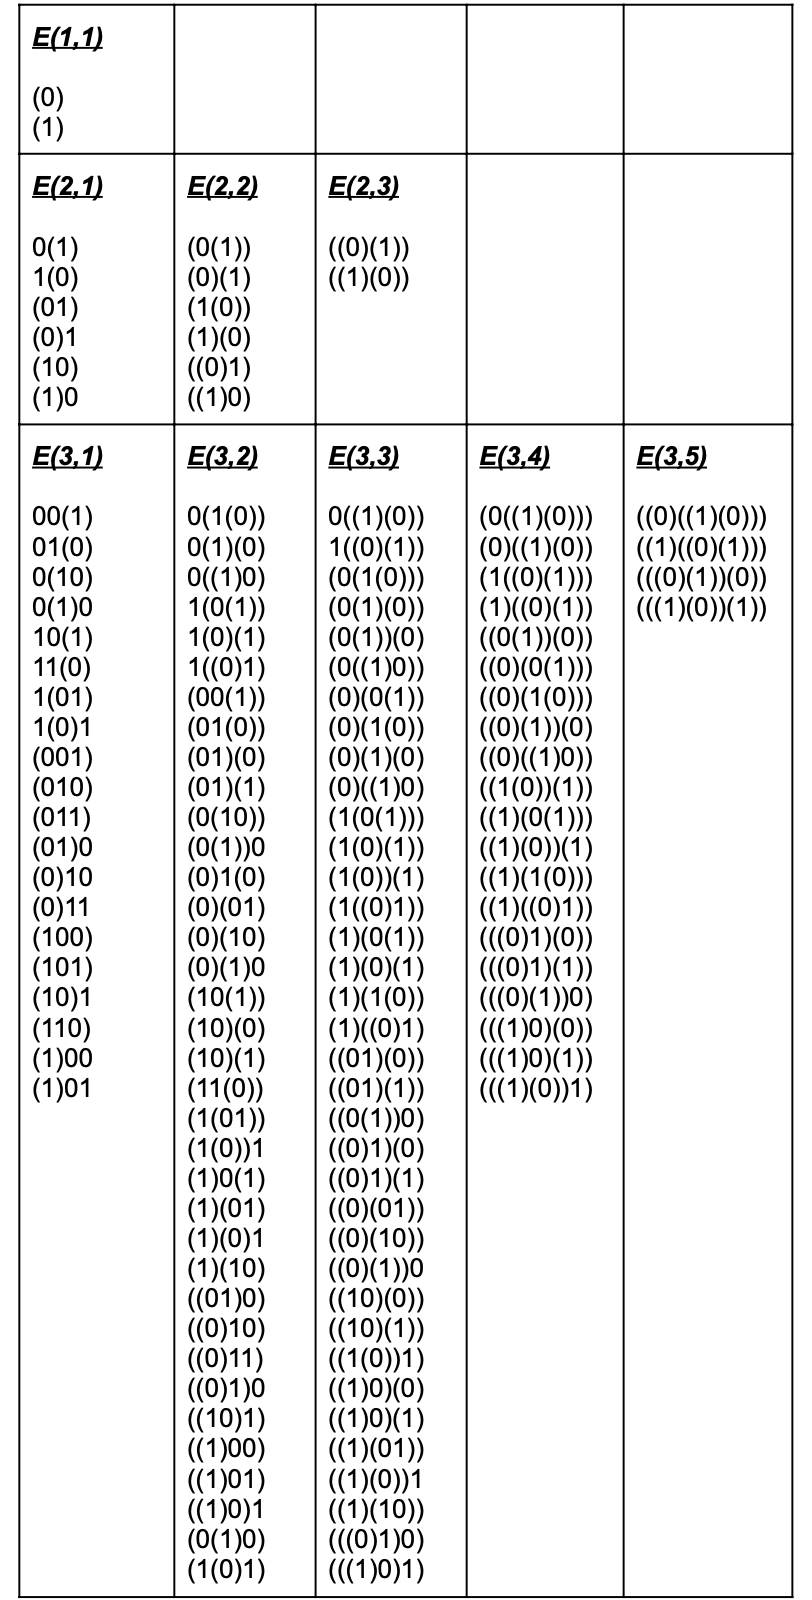
\includegraphics[width=\linewidth]{appendix/sef-seq.png}
    \end{subfigure}
    \caption{Ordered list of equivalence class labels of finite SEFs grouped by length and number of brackets}
    \label{fig:sefseq}
  \end{figure}

  \pagebreak
  \subsection{Concatenation of SEFs}
  \begin{figure}[h!]
    \centering
    \begin{subfigure}[b]{1.0\linewidth}
      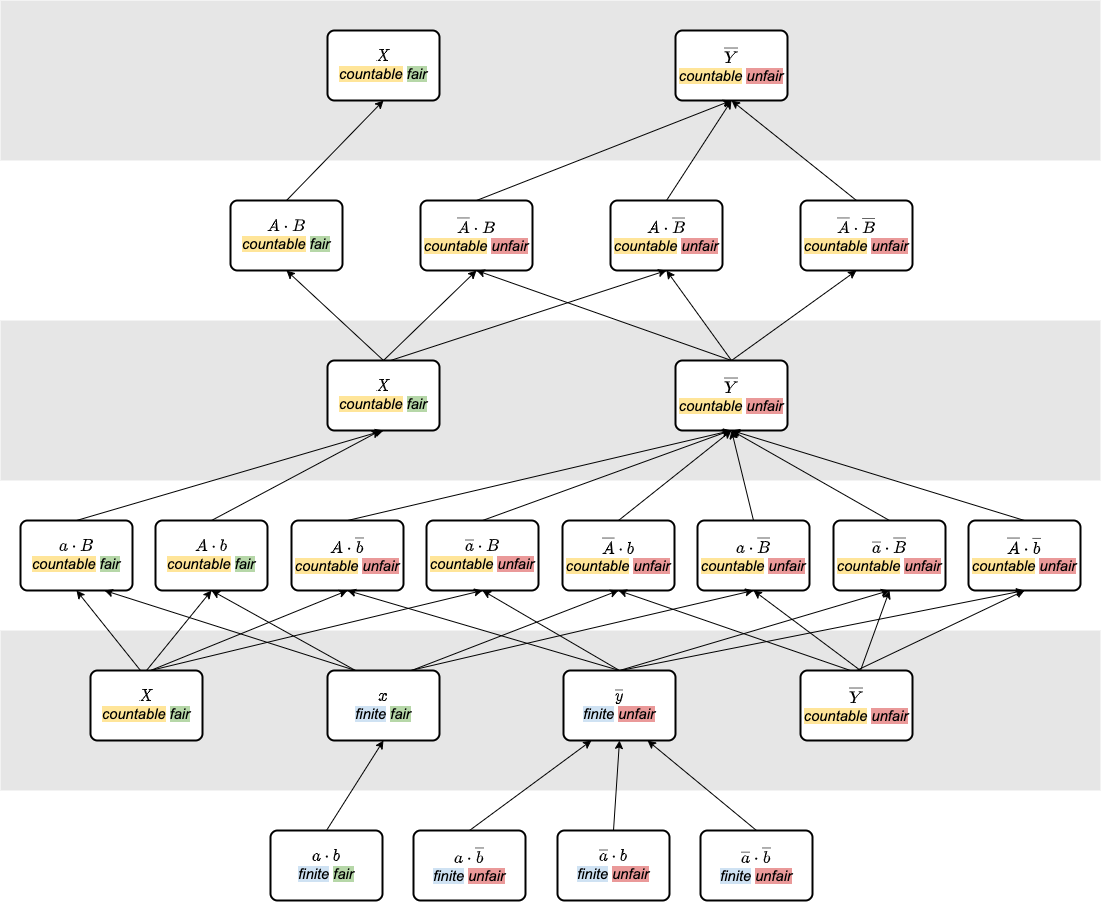
\includegraphics[width=\linewidth]{appendix/concat-hasse-large.png}
    \end{subfigure}
    \caption{Large Hasse-like diagram for SEF concatenation}
    \label{fig:concatlarge}
  \end{figure}

  \pagebreak
  \begin{figure}[h!]
    \centering
    \begin{subfigure}[b]{0.8\linewidth}
      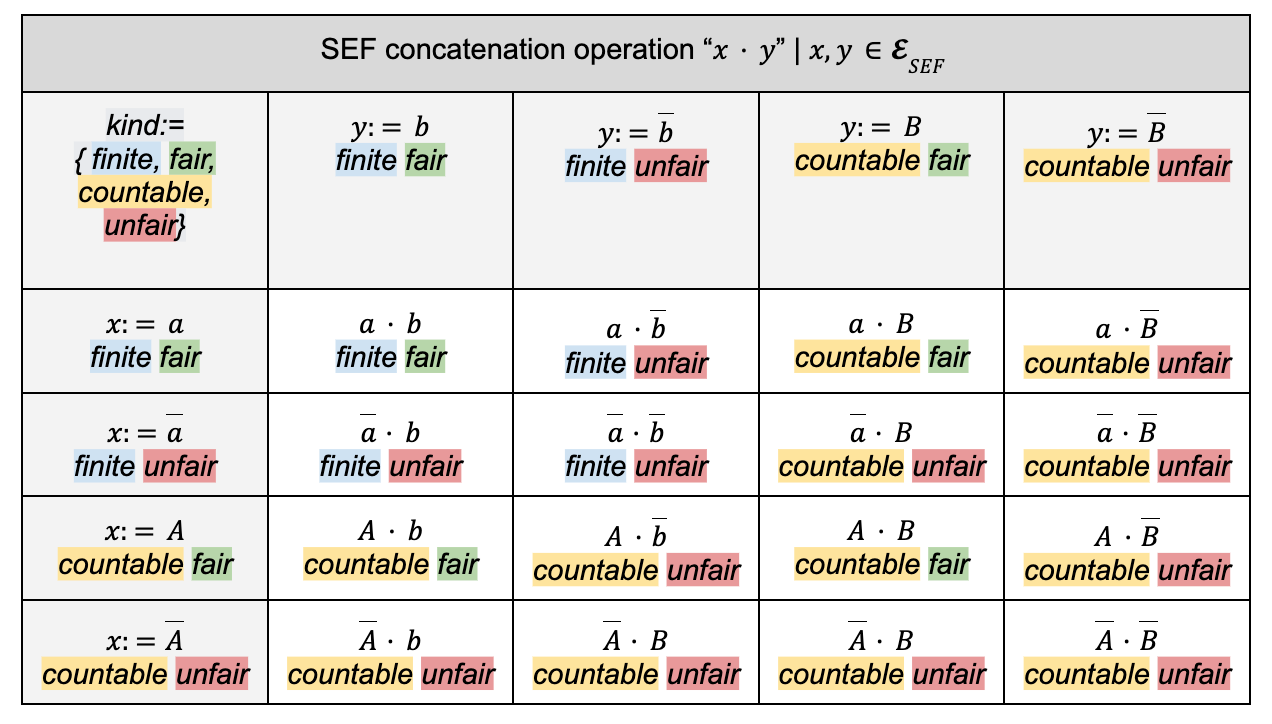
\includegraphics[width=\linewidth]{appendix/concat-table.png}
    \end{subfigure}
    \caption{Table for SEF concatenation operation}
    \label{fig:concattab}
  \end{figure}

  \begin{figure}[h!]
    \centering
    \begin{subfigure}[b]{0.5\linewidth}
      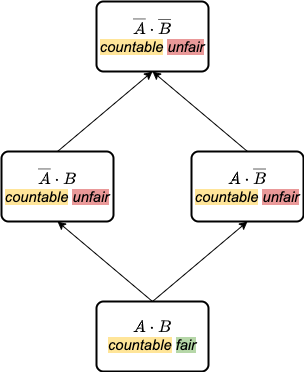
\includegraphics[width=\linewidth]{appendix/concat-hasse-countable.png}
    \end{subfigure}
    \caption{Hasse-like diagram for concatenation of countable SEFs}
    \label{fig:concatcount}
  \end{figure}

  \pagebreak
  \subsection{Power-string operation}
  \begin{figure}[h!]
    \centering
    \begin{subfigure}[b]{0.8\linewidth}
      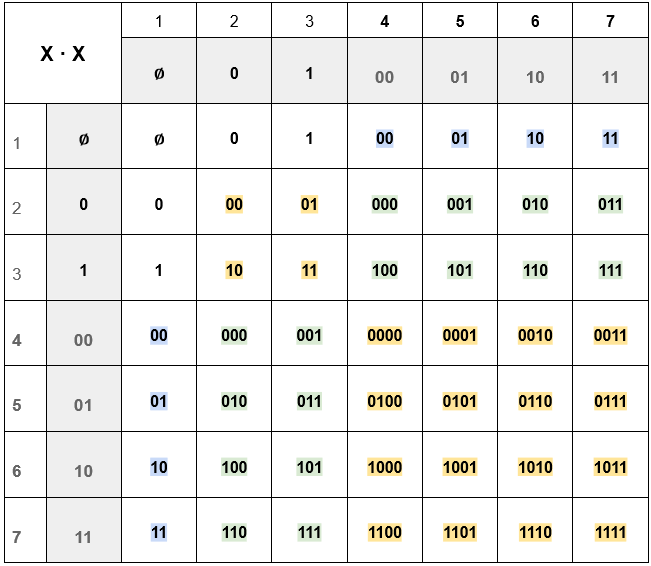
\includegraphics[width=\linewidth]{appendix/power-string.png}
    \end{subfigure}
    \caption{String concatenation table for power-string operation}
    \label{fig:pwrstr}
  \end{figure}

  \begin{table}[ht]
    \caption{Compare power-string and powerset operations}
    \centering
    \begin{tabular}{ |c|r|l| }
      \hline
      \# & power-string $\P(X)$                & powerset $\pset(X)$             \\
      \hline
      0            & $T_0 := \emptyset$        & $V_0 := \emptyset$              \\
      1            & $T_1 := \P(T_0) $         & $V_1 := \pset(V_0)$             \\
      $\dots$      & $\dots $                  & $\dots $                        \\
      $i$          & $T_{i+1} := \P(T_i)$      & $V_{i+1} := \pset(V_{i})$       \\
      \hline
      0            & $|T_0| = 1$               & $|V_0| = 1$                     \\
      1            & $|T_1| = 3$               & $|V_1| = 2$                     \\
      2            & $|T_2| = 7$               & $|V_2| = 4$                     \\
      3            & $|T_3| = 31$              & $|V_3| = 16$                    \\
      4            & $|T_4| = 511$             & $|V_4| = 256$                   \\
      5            & $|T_5| = 131071$          & $|V_5| = 65536$                 \\
      6            & $|T_6| = 8589934591$      & $|V_6| = 4294967296$            \\
      $\dots$      & $\dots $                  & $\dots $                        \\
      $i>0$        & $|T_i| = 2^{2^{i}} - 1$ & $|V_i| = 2^{2^{i-1}}$             \\
      $\dots$      & $\dots $                  & $\dots $                        \\
      \hline
    \end{tabular}
    \label{Tab:PwrStrVsSet}
  \end{table}
  
  \pagebreak
  \subsection{Power-string example in python}
  \lstinputlisting[language=Python]{appendix/pwr-str.py}

  \pagebreak
  \subsection{Set versus String operations}

  \begin{table}[ht]
    \caption{Compare set and string operations}
    \centering
    \begin{tabular}{ |c|c|c| }
      \hline
      \thead{\textbf{set operations}}                                            &  \thead{\textbf{comment}} & \thead{\textbf{string operations}}             \\
      \hline
      \makecell{\\ $x$ is a \textit{member of} $y$: \\ $x \in y$ \\}      &  {\scriptsize is equivalent to} & \makecell{\\ $x$ is a \textit{substring of} $y$: \\ $x \substr y$ \\}   \\
      \hline
      \makecell{\\$y$ is a \textit{subset of} $z$: \\ $y \subset z$ \\ {\tiny or equivalently} \\ $\forall x . [ x \in y \implies x \in z]$ \\}      & {\scriptsize is equivalent to} & \makecell{\\ $y$ is \textit{included in} $z$: \\ $y \Subset  z$ \\ {\tiny or equivalently} \\ $\forall x . [ x \substr y \implies x \substr z]$ \\ {\tiny or equivalently} \\ $\forall x . [ x \in \S(y) \implies x \in \S(z)]$ \\}   \\
      \hline
      \makecell{\\ $s$ is a \textit{union of} $c$: \\ $s = \bigcup c$ \\}  &  \makecell{\\ {\scriptsize \textit{set union}} \\ {\scriptsize is equivalent to} \\ {\scriptsize \textit{class of strings union},} \\ {\scriptsize but not to the \textit{join} which is} \\ {\scriptsize the opposite of \textit{split}} \\} &  \makecell{\\ $[j]$ is a \textit{join of} $z$: \\ $[j] = \mathbb{J}_{s_1, s_2} z$ \\ {\tiny or equivalently} \\ $[j]$ is an equivalence class, s.t. $\forall j \in [j]:$ \\ $\forall x,y . [ x,y \in \S_{s_2}(z) \implies x \cdot s_1 \cdot y \substr j ]$,\\ where $s_1, s_2 \in \Upsilon$ are separators \\}   \\
      \hline
      \makecell{\\$y$ is a \textit{powerset of} $x$: \\ $y = \pset(x)$ \\} & {\scriptsize is equivalent to} & \makecell{\\ $y$ is a \textit{power-string of} $x$: \\ $y = \P(x)$ \\}   \\
      \hline
    \end{tabular}
    \label{Tab:CmpSetVsStrOps}
  \end{table}

  \pagebreak
  \subsection{Examples of recursive Kuratowski notation}

  Given the recursive version of the Kuratowski notation as provided in \textit{Definition \ref{def_kuratowski_morph}}, let us illustrate how it encodes string concatenation to represent strings as sets.

  \begin{table}[ht]
    \caption{String concatenation encoded as sets}
    \centering
    \begin{tabular}{ |c|c|c| }
      \hline
      \thead{\textbf{Tuple/String}} & \thead{\textbf{Tuple/String Encoding}} & \thead{\textbf{Kuratowski Notation}} \\
      \hline
      x = (a,b) & "ab" & $\{\{a\}, \{a, b\}\}$ \\
      y = (c,d) & "cd" & $\{\{c\}, \{c, d\}\}$ \\
      z = x$\cdot$y & "abcd" & \makecell{$\{\{\{\{a\}, \{a, b\}\}, \{c\}\}$, \\ $\{\{\{a\}, \{a, b\}\}, \{c\}\}, d\}\}$ } \\
      \hline
    \end{tabular}
    \label{Tab:ExmplRecKurMorph}
  \end{table}

  Again, note that the complexity of the notation for $\bos abcd \eos$ arises from the recursive structure of the \textit{Definition \ref{def_kuratowski_morph}}. The more elements in the sequence, the more nested the notation becomes.

  \pagebreak
  \subsection{Acknowledgements}

  Significant part of the paper is written in informal style \footnote{including a lot of footnotes and references for non-specialists} with genuine intention to make the discussion a bit more accessible to the wider audience. The disadvantage of this approach is that it often comes at cost of discussing trivialities or even lack of expected rigor in claims. So all of this obviously needs further careful verification and improvement to avoid any potential confusion\footnote{please expect version updates of this paper}. However, author firmly believes that all the presented results are overall correct and will contribute to novel developments in the respective fields.

  Much love, credit and gratitude goes to all cited sources which have been both inspiring and insightful. This also includes many kinds of online discussion forums and resources on mathematics such as wikipedia and youtube, that have not been cited well enough. Special thanks to the communities of math.stackexchange and mathoverflow forums with all the helpful posts on basic results in Set Theory. 

  Finally, sincere sense of gratitude goes to a transitive set of all mathematicians - dead, living or future ones. Author wants to thank the audience for their patience. Comments or remarks are welcomed per email correspondence.

\end{appendices}


\end{document}
